%\documentclass[12pt]{report}
\documentclass[a4paper,12pt,oneside]{book}
%\usepackage[a4paper, margin=2cm, footskip=15pt]{geometry}
\usepackage[a4paper,top=3.5cm,left=3cm,right=3cm,bottom=2.5cm]{geometry}
\usepackage{times} %pacote da fonte Times New Roman
\usepackage[utf8]{inputenc}
\usepackage[export]{adjustbox}
\usepackage{caption}
\usepackage{subcaption}
\usepackage{setspace}
\usepackage{indentfirst}
\usepackage{float}
\usepackage{amsmath}
\usepackage{appendix}
%\usepackage{pgfplots}
% \usepackage{unicode-math}
\newcommand\mathplus{+}
% \usepackage{subfigure}
% \usepackage{algorithm}
% \usepackage[ruled,vlined,lined,linesnumbered,spanish, onelanguage]{algorithm2e}
\usepackage[ruled,vlined,lined,linesnumbered,portuguese, onelanguage]{algorithm2e}
% \usepackage{algorithmic}
\usepackage{algpseudocode}
\renewcommand{\baselinestretch}{1.3}
\usepackage[backend=bibtex, style=numeric, sorting=none]{biblatex}
\addbibresource{sample.bib}
%\renewcommand{\listalgorithm}{Lista de Algoritmos}%
%\renewcommand{\algorithm}{Algoritmo}%
%\renewcommand{\algocf@typo}{}%
%\renewcommand{\@algocf@procname}{Procedimento}
%\renewcommand{\@algocf@funcname}{Fun\c{c}\~{a}o}
\usepackage[scr=rsfs]{mathalpha}
\DeclareMathOperator{\sinc}{sinc}
\DeclareMathOperator{\rect}{rect}
\DeclareMathOperator{\atantwo}{atan2}

\usepackage{hyperref}
\hypersetup{colorlinks=false, pdftitle={Tese}}
% \usepackage[backend=biber]{biblatex}
% \addbibresource{sample.bib}
\renewcommand\appendixname{Apêndice}
\renewcommand\appendixpagename{Apêndices}




\begin{document}
\pagestyle{plain}
\captionsetup[figure]{name={Figura}}
\renewcommand*\contentsname{Sumário}
\renewcommand{\listfigurename}{Lista de figuras}
\renewcommand{\listoftables}{Tabelas}
\renewcommand{\listofalgorithms}{Lista de algoritmos}
\makeatletter
\renewcommand{\@chapapp}{Capítulo}
\makeatother



\thispagestyle{empty}
\begin{center}

%%%%%%%%%%%%%%%%%%%%%%%%%%%%%%%%%%%%%%%%%%%%%%%%%%%%%%%%%%%%%%%%%%%%%%%%%%%%%%%%%%%%%    
%\Título da Tese \ Thesis title
	{\fontsize{16}{16} \selectfont Universidade de S\~ao Paulo \\}
	\vspace{0.1cm}
	{\fontsize{16}{16} \selectfont Instituto de F\'{i}sica}
    \vspace{2.2cm}

	{\fontsize{22}{22}\selectfont Estudo da reação de breakup $^4$He($^{17}$F,$^{16}$O+p)$^4$He usando o alvo ativo pAT-TPC: uma abordagem usando técnicas de Machine Learning\par}
    \vspace{2cm}

%%%%%%%%%%%%%%%%%%%%%%%%%%%%%%%%%%%%%%%%%%%%%%%%%%%%%%%%%%%%%%%%%%%%%%%%%%%%%%%%%%%%%    
%\Nome do Autor \ Author's name

    {\fontsize{18}{18}\selectfont Guilherme Ferrari Fortino\par}

    \vspace{1.4cm}

\end{center}

%%%%%%%%%%%%%%%%%%%%%%%%%%%%%%%%%%%%%%%%%%%%%%%%%%%%%%%%%%%%%%%%%%%%%%%%%%%%%%%%%%%%%%    
%\Orientador e coorientador (se existir) \ Supervisor and co-supervisor (if there is one)
\leftskip 6cm
\begin{flushright}	
\leftskip 6cm
Orientador: Prof. Dr.  Valdir Guimarães\underline{ \hskip 5cm  } 
\leftskip 6cm
    %Se não houve coorientador, comente a linha abaixo \ If there is no co-advisor, comment line below
Coorientador: Dr. Juan Carlos Zamora Cardona  \underline{ \hskip 5cm  } 
\end{flushright}	

\vspace{0.6cm}    

%%%%%%%%%%%%%%%%%%%%%%%%%%%%%%%%%%%%%%%%%%%%%%%%%%%%%%%%%%%%%%%%%%%%%%%%%%%%%%%%%%%%%    
% Grau Acadêmico \ Degree

\par
\leftskip 6cm
\noindent {Disserta\c{c}\~{a}o de mestrado apresentada ao Instituto de F\'{i}sica da Universidade de S\~{a}o Paulo, como requisito parcial para a obten\c{c}\~{a}o do t\'{i}tulo de Mestre(a) em Ci\^{e}ncias.}
\par
\leftskip 0cm
\vskip 2cm

%%%%%%%%%%%%%%%%%%%%%%%%%%%%%%%%%%%%%%%%%%%%%%%%%%%%%%%%%%%%%%%%%%%%%%%%%%%%%%%%%%%%    
% Banca Examinadora -- Primeiro nome é do presidente ou do presidente da banca \ Examining committee -- The first name must be the supervisor's name or the examination committee president's name.

\noindent Banca Examinadora: \\
\noindent Prof(a). Dr(a). Nome do(a) Professor(a) - Orientador (institui\c{c}\~{a}o de trabalho) \\
Prof(a). Dr(a). Nome do(a) Professor(a) (institui\c{c}\~{a}o de trabalho) \\
Prof(a). Dr(a). Nome do(a) Professor(a) (institui\c{c}\~{a}o de trabalho) \\
\vspace{1.8cm}


%%%%%%%%%%%%%%%%%%%%%%%%%%%%%%%%%%%%%%%%%%%%%%%%%%%%%%%%%%%%%%%%%%%%%%%%%%%%%%%%%%%%    
%Data \ Date
\begin{center}
    {S\~ao Paulo \\  2022}
\end{center}%\centering
    
\clearpage

\tableofcontents
\listoffigures
\listoftables
\listofalgorithms
\newpage

\chapter{Introdução}


\par Um dos principais objetivos do estudo em física nuclear é entender a estrutura do núcleo. Apesar do sucesso do modelo de camadas em explicar as estruturas de núcleos estáveis, os núcleos instáveis ou exóticos, ricos ou pobres em nêutrons, continuam sendo um grande desafio para nossa compreensão.

\par Os núcleos leves radioativos são de grande interesse para a astrofísica nuclear \cite{BARDAYAN2017415}, onde processos de captura rápida de nêutrons e prótons (que ocorrem em eventos explosivos de novas ou supernovas) envolvem os núcleos radioativos longe da linha de estabilidade. Conhecer as propriedades desses núcleos, como massa, probabilidades de decaimento, seções de choque de captura e de \textit{breakup} é fundamental para o entendimento da vários eventos astrofísicos \cite{BARDAYAN2017415, abud_mater}. A figura \ref{fig:chart_nuclides} mostra parte da tabela de nuclídeos, onde é mostrado núcleos longe da linha de estabilidade, com a informação da energia de separação do próton ($S_p$).

\begin{figure}[H]
    \centering
    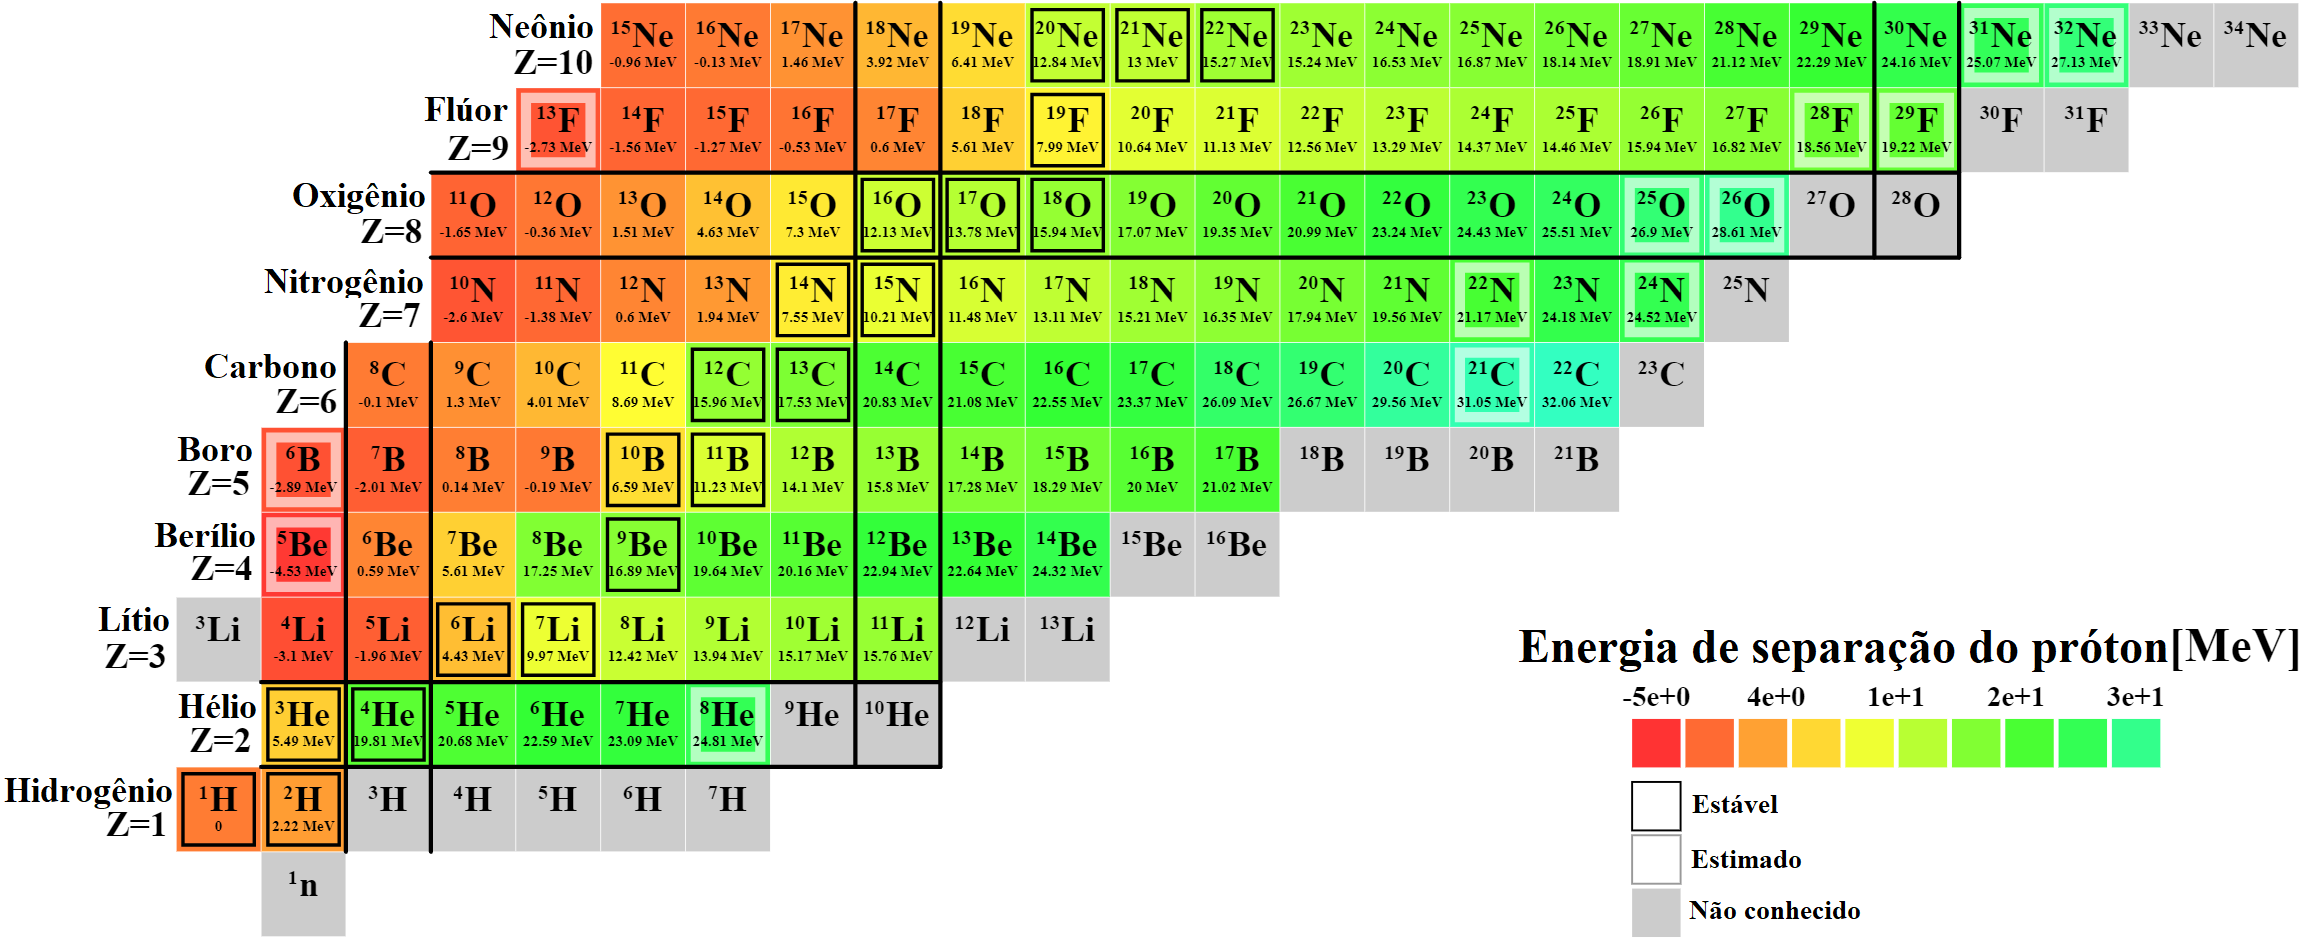
\includegraphics[scale = 0.25]{figs/chart_nuclides.png}
    \caption{Tabela de nuclídeos para elementos leves, indicando a energia de separação de um próton em MeV. O núcleo estudado nesse trabalho é o $^{17}$F, com $S_p$ = 600 keV. \cite{colourful_nuclide_chat}}
    \label{fig:chart_nuclides}
\end{figure}

\par Para investigar a estrutura de núcleos ricos em prótons ou em nêutrons, é possível usar reações nuclear como espalhamento elástico, transferência e breakup \cite{Kolata2016}. A reação de breakup é a reação nuclear tal que o projétil ao interagir com o alvo, se dissocia em seus constituintes \cite{Kolata2016, MORO_BREAKUP}. A reação estudada nessa dissertação é a reação de breakup $^4$He($^{17}$F,$^{16}$O+p)$^4$He, onde o $^{17}$F é um núcleo próton-halo que pode ser descrito como um núcleo de $^{16}$O mais um próton fracamente ligado ($S_p$ = 600 keV) \cite{MORO_BREAKUP}.

\par Para a investigação de reação nuclear de breakup, é importante identificar todas as partículas que se quebraram, necessitando de um sistema de detecção sofisticado, como o alvo ativo. O alvo ativo é um sistema detector que funciona tanto quanto meio detector quanto alvo de reações nucleares. Com o alvo ativo, é possível determinar as trajetórias das partículas presentes antes e depois de reações nucleares, sendo de grande interesse para medir reações de breakup. Na experiência, o alvo ativo utilizado foi o gás $^4$He.

\par Nos últimos anos, câmaras de projeção no tempo com alvos ativos, \textit{ative-target time projection chambers} (ATTPCs), se tornaram importantes e relevantes para o estudo de núcleos exóticos em física nuclear \cite{FORTINO2022166497}. Diversos projetos de TPCs foram desenvolvidos em diferentes laboratórios de física nuclear pelo mundo \cite{attpc, FURUNO2018215, KOSHCHIY2020163398}. O alvo ativo permite o uso de um gás específico que serve tanto quanto alvo quanto meio detector. Isso permite a detecção de múltiplas reações nucleares ao mesmo tempo, com a capacidade de medidas completas da cinemática das reações \cite{FORTINO2022166497, josh_bradt, attpc}. Com a cinemática completa é possível identificar o mecanismo de reação e obter as seções de choque.

\par O sistema de detecção de TPCs, usualmente, é baseado no \textit{Micro-MEsh GAseous Structures} (MICROMEGAS) \cite{micromegas} e no 
Gas Electron Multiplier (GEM) \cite{GET}, que possui alta granularidade do plano detector, da ordem de 10$^3$ a 10$^4$ canais \cite{FORTINO2022166497}. Experimentos que envolvem o TPC produzem enormes quantidades, onde, por exemplo, uma semana de experimento com o \textit{Active Target - Target Projection Chamber} (AT-TPC) produz cerca de 10 TB de dados \cite{attpc, pattpc}. Devido à grande quantidade de dados produzidos, a análise precisa ser dividida em diversas etapas, de modo que a eficiência e tempo computacional têm papel fundamental no processo. Diversos algoritmos foram desenvolvidos para a análise de diferentes etapas dos dados \cite{FORTINO2022166497, artigo}, porém o uso de algoritmos de \textit{machine learning} pode trazer vantagens significativas para a análise. Um dos objetivos desse trabalho foi o de desenvolver técnicas para a análise desses dados produzidos.

\par Este trabalho abordou a análise do experimento feito com o \textit{prototype Active Target - Time Projection Chamber} (pAT-TPC) \cite{pattpc} usando técnicas de \textit{machine learning}. Os algoritmos de \textit{machine learning} viabilizaram análises mais rápidas em comparação à algoritmos mais tradicionais. O trabalhou, até a data em que a dissertação foi escrita, resultou nos artigos encontrados nas Refs. \cite{artigo, FORTINO2022166497}.

\par A dissertação está esquematizada da seguinte forma: no capítulo \ref{PATTPC} está feita a descrição do experimento; no capítulo \ref{sec:ml} está feita uma breve descrição do que é \textit{machine learning} com exemplos de aplicações em física nuclear; O capítulo \ref{chapter:sinais} foi dedicado para a análise dos sinais (pulsos) gerados no experimento; No capítulo \ref{chapter:point_cloud_analysis} está descrita a análise das nuvens de pontos reconstruídas a partir dos sinais; No capítulo \ref{chapter:resultados} foi feita a construção das distribuições angulares; Por fim, no capítulo \ref{chapter:conclusao} está a conclusão do trabalho.

\chapter{O experimento}\label{PATTPC}

%\par Esse capítulo descreve sobre a parte experimental desse trabalho que foi desenvolvido na Universidade de Notre Dame em Outubro de 2019. O experimento foi feito usando o feixe radioativo $^{17}$F produzido pelo sistema TWINSOL (TWIN SOLenids) \cite{twinsol} e o alvo ativo pAT-TPC \textit{prototype Active Target - Time Projection Chamber} \cite{pattpc} foi usando como alvo e detector simultaneamente. Na continuação, está descrito como foi feito o sistema de produção do feixe secundário $^{17}$F e a detecção das reações induzidas por esse feixe no alvo ativo.

\par Esse trabalho corresponde a analise de dados obtidos da experiência onde foi medida a reação de breakup para o $^{17}$F+$^{4}$He. Neste capítulo, está descrito como o feixe radioativo de 17F foi obtido e como os fragmentos da reação de breakup foram medidos. A experiência foi realizada em outubro de 2019 na University of Notre Dame, Estados. Unidos. O feixe radioativo de $^{17}$F foi obtido como sistema de produção chamado TWINSOL (TWIN SOLenids) \cite{twinsol} e conduzido até o alvo ativo pAT-TPC \textit{prototype Active Target - Time Projection Chamber} \cite{pattpc}.

% \par Primeiro será descrita a produção do feixe de $^{17}$F com foco na descrição do sistema de produção de feixes radioativos (TWINSOL). Na seção seguinte será apresentado o detector pAT-TPC.


% O objetivo deste experimento é fazer medidas do \textit{breakup} do  gasoso, com o prototype Active Target - Time Projection Chamber (pAT-TPC). Esse capítulo irá descrever a produção do feixe e a 

% \par O prototype Active Target - Time Projection Chamber (pAT-TPC) é um detector de alvo-ativo que usa o volume de gás tanto quanto alvo quanto como detector. Seu grande volume ativo e capacidade de rastreio (\textit{tracking}) fornecem boa resolução energética e  angular, o que torna o pAT-TPC adequado para trabalhar com feixes exóticos de baixa intensidade\cite{pattpc, pattpc2}. O feixe secundário de $^{17}$F usado pelo pAT-TPC é produzido pelo \textit{Twin Solenoids} (TWINSOL) \cite{twinsol}. A figura \ref{fig:twinsol+pattpc} mostra os dois sistemas acoplados.

% \par Essa seção irá descrever brevemente o pAT-TPC, bem como o TWINSOL. Descrições mais detalhadas podem ser encontradas nas referências \cite{pattpc, twinsol}.

% \section{Produção do feixe de $^{17}$F}
\section{Produção do feixe secundário $^{17}$F usando o sistema TWINSOL}\label{sec:twinsol}

\par Nesse sistema o feixe de $^{17}$F é produzido em voo \cite{KOLATA1989503, NDtandem}. Um feixe de $^{16}$O é acelerado a uma energia de 70 MeV e intensidade de 10$^4$ $\sim$ 10$^5$ partículas por segundo e é conduzido até a câmara de produção. Nessa câmara temos um alvo de produção que consiste de uma célula gasosa, preenchida com gás de deutério à uma pressão de 1 atm. A partir da reação do feixe primário com o alvo de produção (deutério), partículas como $^{17}$F, $^{17}$O, são produzidas a partir de reações nucleares de transferência \cite{KOLATA1989503, twinsol}. Essas partículas são selecionadas com um sistema de duplo solenoides \cite{twinsol, ribras_leo}. A figura \ref{fig:twinsol+pattpc} mostra o sistema TWINSOL acoplado com o pAT-TPC.

%\par A produção do feixe radioativo $^{17}$F foi feita a partir da reação do feixe estável de $^{16}$O com um alvo de deutério gasoso. O feixe primário $^{16}$O foi produzido e acelerado por um acelerador tipo Tandem van de Graff do ISNAP (\textit{Institute for Structure and Nuclear Astrophysics}) localizado na Universidade de Notre Dame, Estados Unidos, que possui uma tensão terminal de até 10 MV \cite{KOLATA1989503, NDtandem}. O feixe de $^{16}$O foi conduzido até a câmara alvo de produção, preenchida com deutério, no início do sistema TWINSOL, onde partículas emergentes de reações nucleares surgiram ($^{17}$F, $^{16}$O, $^{17}$O). A figura \ref{fig:twinsol+pattpc} mostra o sistema TWINSOL acoplado com o pAT-TPC.

\begin{figure}[H]
    \centering
    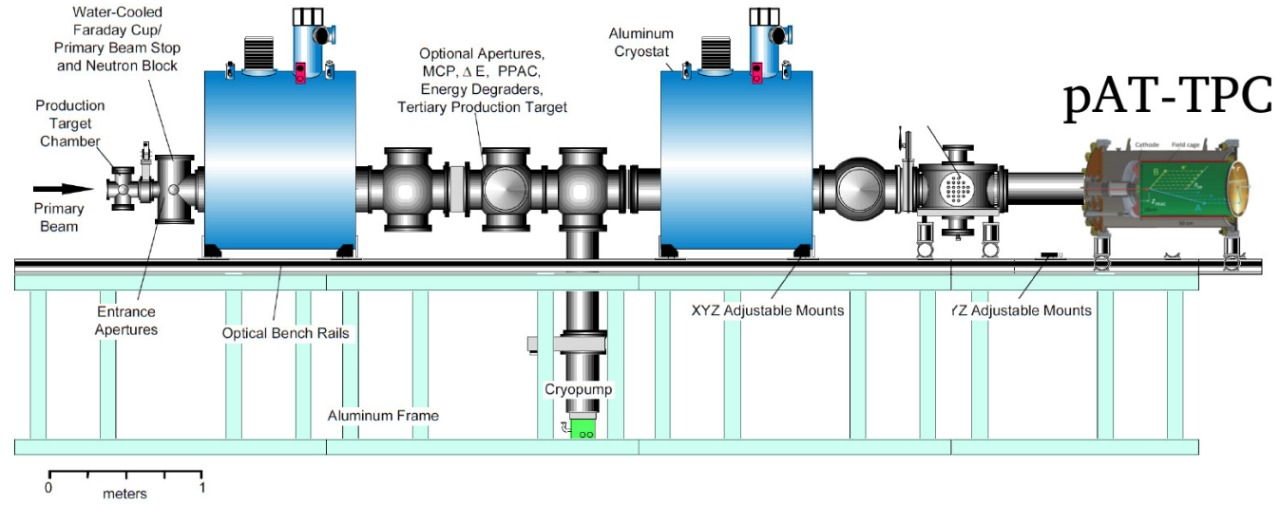
\includegraphics[scale = 0.35]{figs/poster3.jpeg}
    \caption{Sistema TWINSOL à esquerda e pAT-TPC à direita. O feixe estável de $^{16}$O entra à esquerda do TWINSOL, para então ser produzido o feixe secundário $^{17}$F que irá ser conduzido até o alvo ativo pAT-TPC. Todo o sistema está localizado na University of Notre Dame.}
    \label{fig:twinsol+pattpc}
\end{figure}

\par O TWINSOL é um sistema de produção de feixes radioativos em voo que possui dois solenoides supercondutores alinhados que são usados para produzir, coletar, transportar, focar e analisar feixes estáveis e radioativos. O sistema se baseia na seleção de partículas a partir da sua rigidez magnética ($B\rho$) \cite{twinsol, ribras_leo, zamora_mater}. Cada solenoide possui 30 cm de raio interno e 1 m de comprimento \cite{twinsol}. O fato de ser um solenoide finito faz com que surjam efeitos de borda na componente radial do campo magnético do solenoide, cujo efeito faz com que o solenoide seja capaz de focalizar partículas. Para entender melhor o efeito de borda no campo magnético, e consequentemente o funcionamento do TWINSOL, simulações computacionais usando a biblioteca GEANT4 \cite{geant4} foram feitas usando a geometria do sistema ``irmão" do TWINSOL, o Radioactive Ion Beams in Brasil (RIBRAS), que também possui dois solenoides supercondutores alinhados \cite{ribras_leo, ribras}. A figura \ref{fig:sim_ribras} mostra a geometria usada na simulação, onde os solenoides são de cor verde focalizando as partículas de cor laranja em um ponto do plano focal em vermelho. O campo magnético usado na simulação é função da posição do eixo, de cada solenoide, e está mostrado na figura \ref{fig:campo_mag}.


% A figura  mostra um exemplo de calculo do valor do campo magnético, usando valores do sistema , para as componentes $x$, $y$ e $z$. É nítido que o campo em $z$ permanece praticamente constante e próximo das extremidades da bobina (linha vertical tracejada preta), $B_x$ e $B_y$ crescem em módulo, fazendo com que o solenoide funcione como uma lente delgada.

\begin{figure}[H]
    \centering
    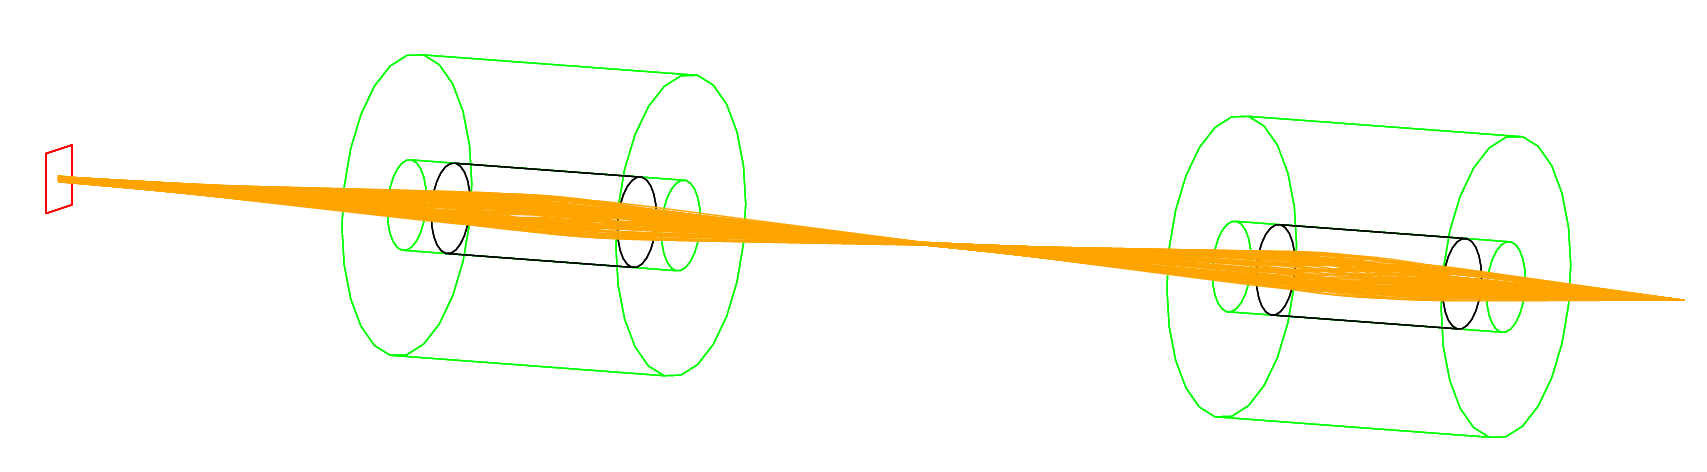
\includegraphics[scale = 0.95]{figs/Foco2S.png}
    \caption{Simulação computacional do sistema RIBRAS, onde as partículas carregas em laranja surgem do ponto à direita da figura e passam pelos dois solenoides em verde, para então serem focalizada em um ponto do plano focal em vermelho. A parte em preto dos solenoides corresponde aos limites físicos da bobina \cite{ribras_leo}.}
    \label{fig:sim_ribras}
\end{figure}

\begin{figure}[H]
    \centering
    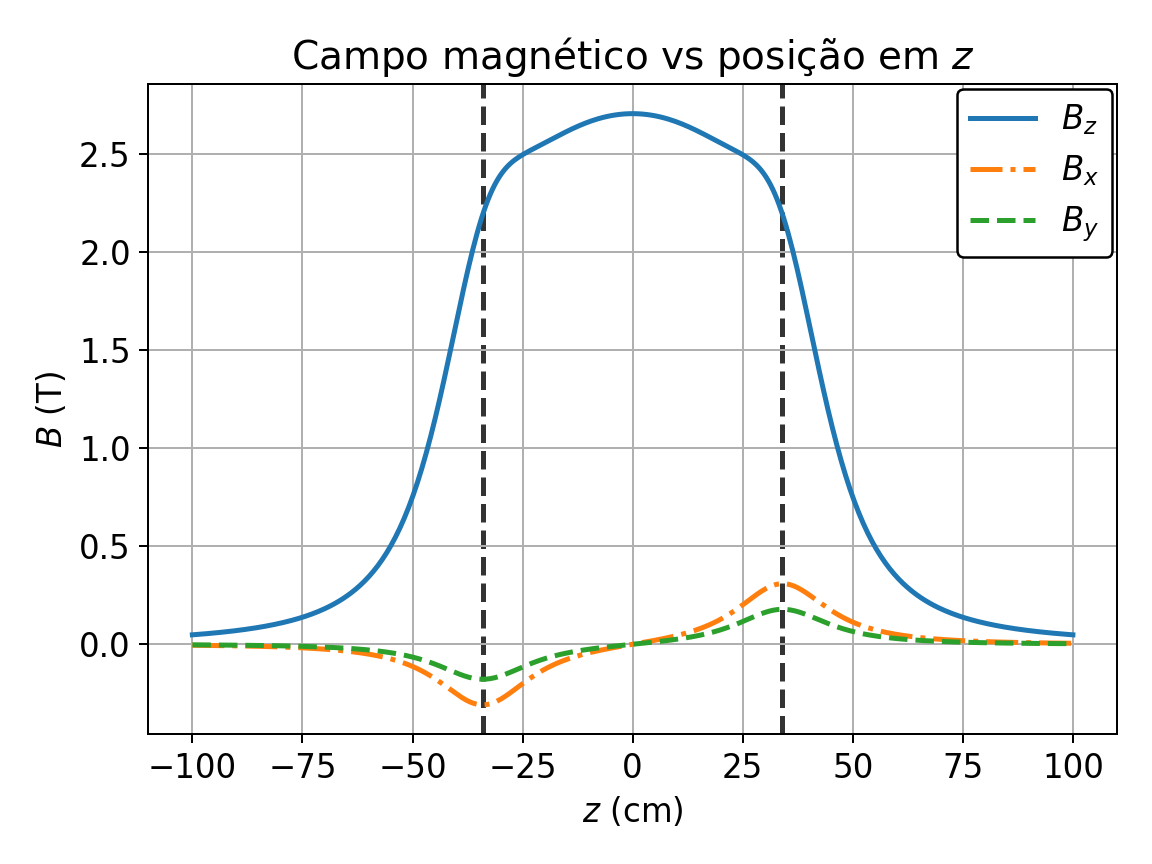
\includegraphics[scale = 0.85]{figs/Campo_mag.png}
    \caption{Valor do campo magnético $B$ em tesla em função da posição em $z$ em centímetro da bobina. A linha vertical tracejada preta indica o limite físico da bobina. O campo foi calculado à uma distância de 8 cm do eixo do solenoide. É possível ver claramente o efeito de borda que há em um solenoide finito \cite{magnetic_field}.}
    \label{fig:campo_mag}
\end{figure}


\par A trajetória as partículas dentro do solenoide são helicoidais devido à força de Lorentz e possuem uma determinada frequência de ciclotron \cite{ribras_leo}. Além disso, cada solenoide é uma lente grossa usada para focalizar os feixes. Em uma aproximação de um solenoide como uma lente grossa, o foco depende da rigidez magnética da partícula através da relação \cite{KOLATA1989503, zamora_mater}:

\begin{equation}
    \frac{1}{f} = \frac{B_z ^2}{(B\rho)^2},
\end{equation}

onde $f$ é o ponto focal, $B_z$ a componente $z$ do campo magnético, e $B\rho$ é dado por:

\begin{equation}
    B\rho = \frac{mv}{q} = \frac{\sqrt{2mE}}{q},
\end{equation}

onde $E$ é a energia, $m$ sua massa e $q$ seu estado de carga.

%\par Para produzir $^{17}$F, uma célula gasosa localizada na câmara alvo de produção\cite{twinsol} preenchida com deutério foi bombardeada pelo feixe primário. Além de $^{17}$F, outras partículas também foram geradas, como o $^{17}$O, além de $^{16}$O do feixe espalhado.

\par No experimento, os campos magnéticos dos solenoides foram ajustados para focalizar o feixe de $^{17}$F dentro do pAT-TPC, produzindo $^{17}$F com energia de 51 MeV e intensidade da ordem de 10$^2$ $\sim$ 10$^3$ partículas por segundo. No entanto, mesmo para partículas diferentes, o $B\rho$ pode ser muito próximo ou igual. Isso faz com que não seja possível obter um feixe de $^{17}$F com 100\% de pureza, e sim um coquetel de partículas \cite{zamora_mater}. O coquetel de partículas produzido possui 54\% de $^{17}$F, 41\% de $^{16}$O e cerca de 5\% de $^{17}$O. A figura \ref{fig:PID_17F} mostra o espectro biparamétrico de identificação de partículas obtido durante o experimento, onde é possível identificar as partículas que estão presentes no feixe (coquetel de partículas). Por fim, o feixe produzido pelo TWINSOL é conduzido até o pAT-TPC.

\begin{figure}[H]
    \centering
    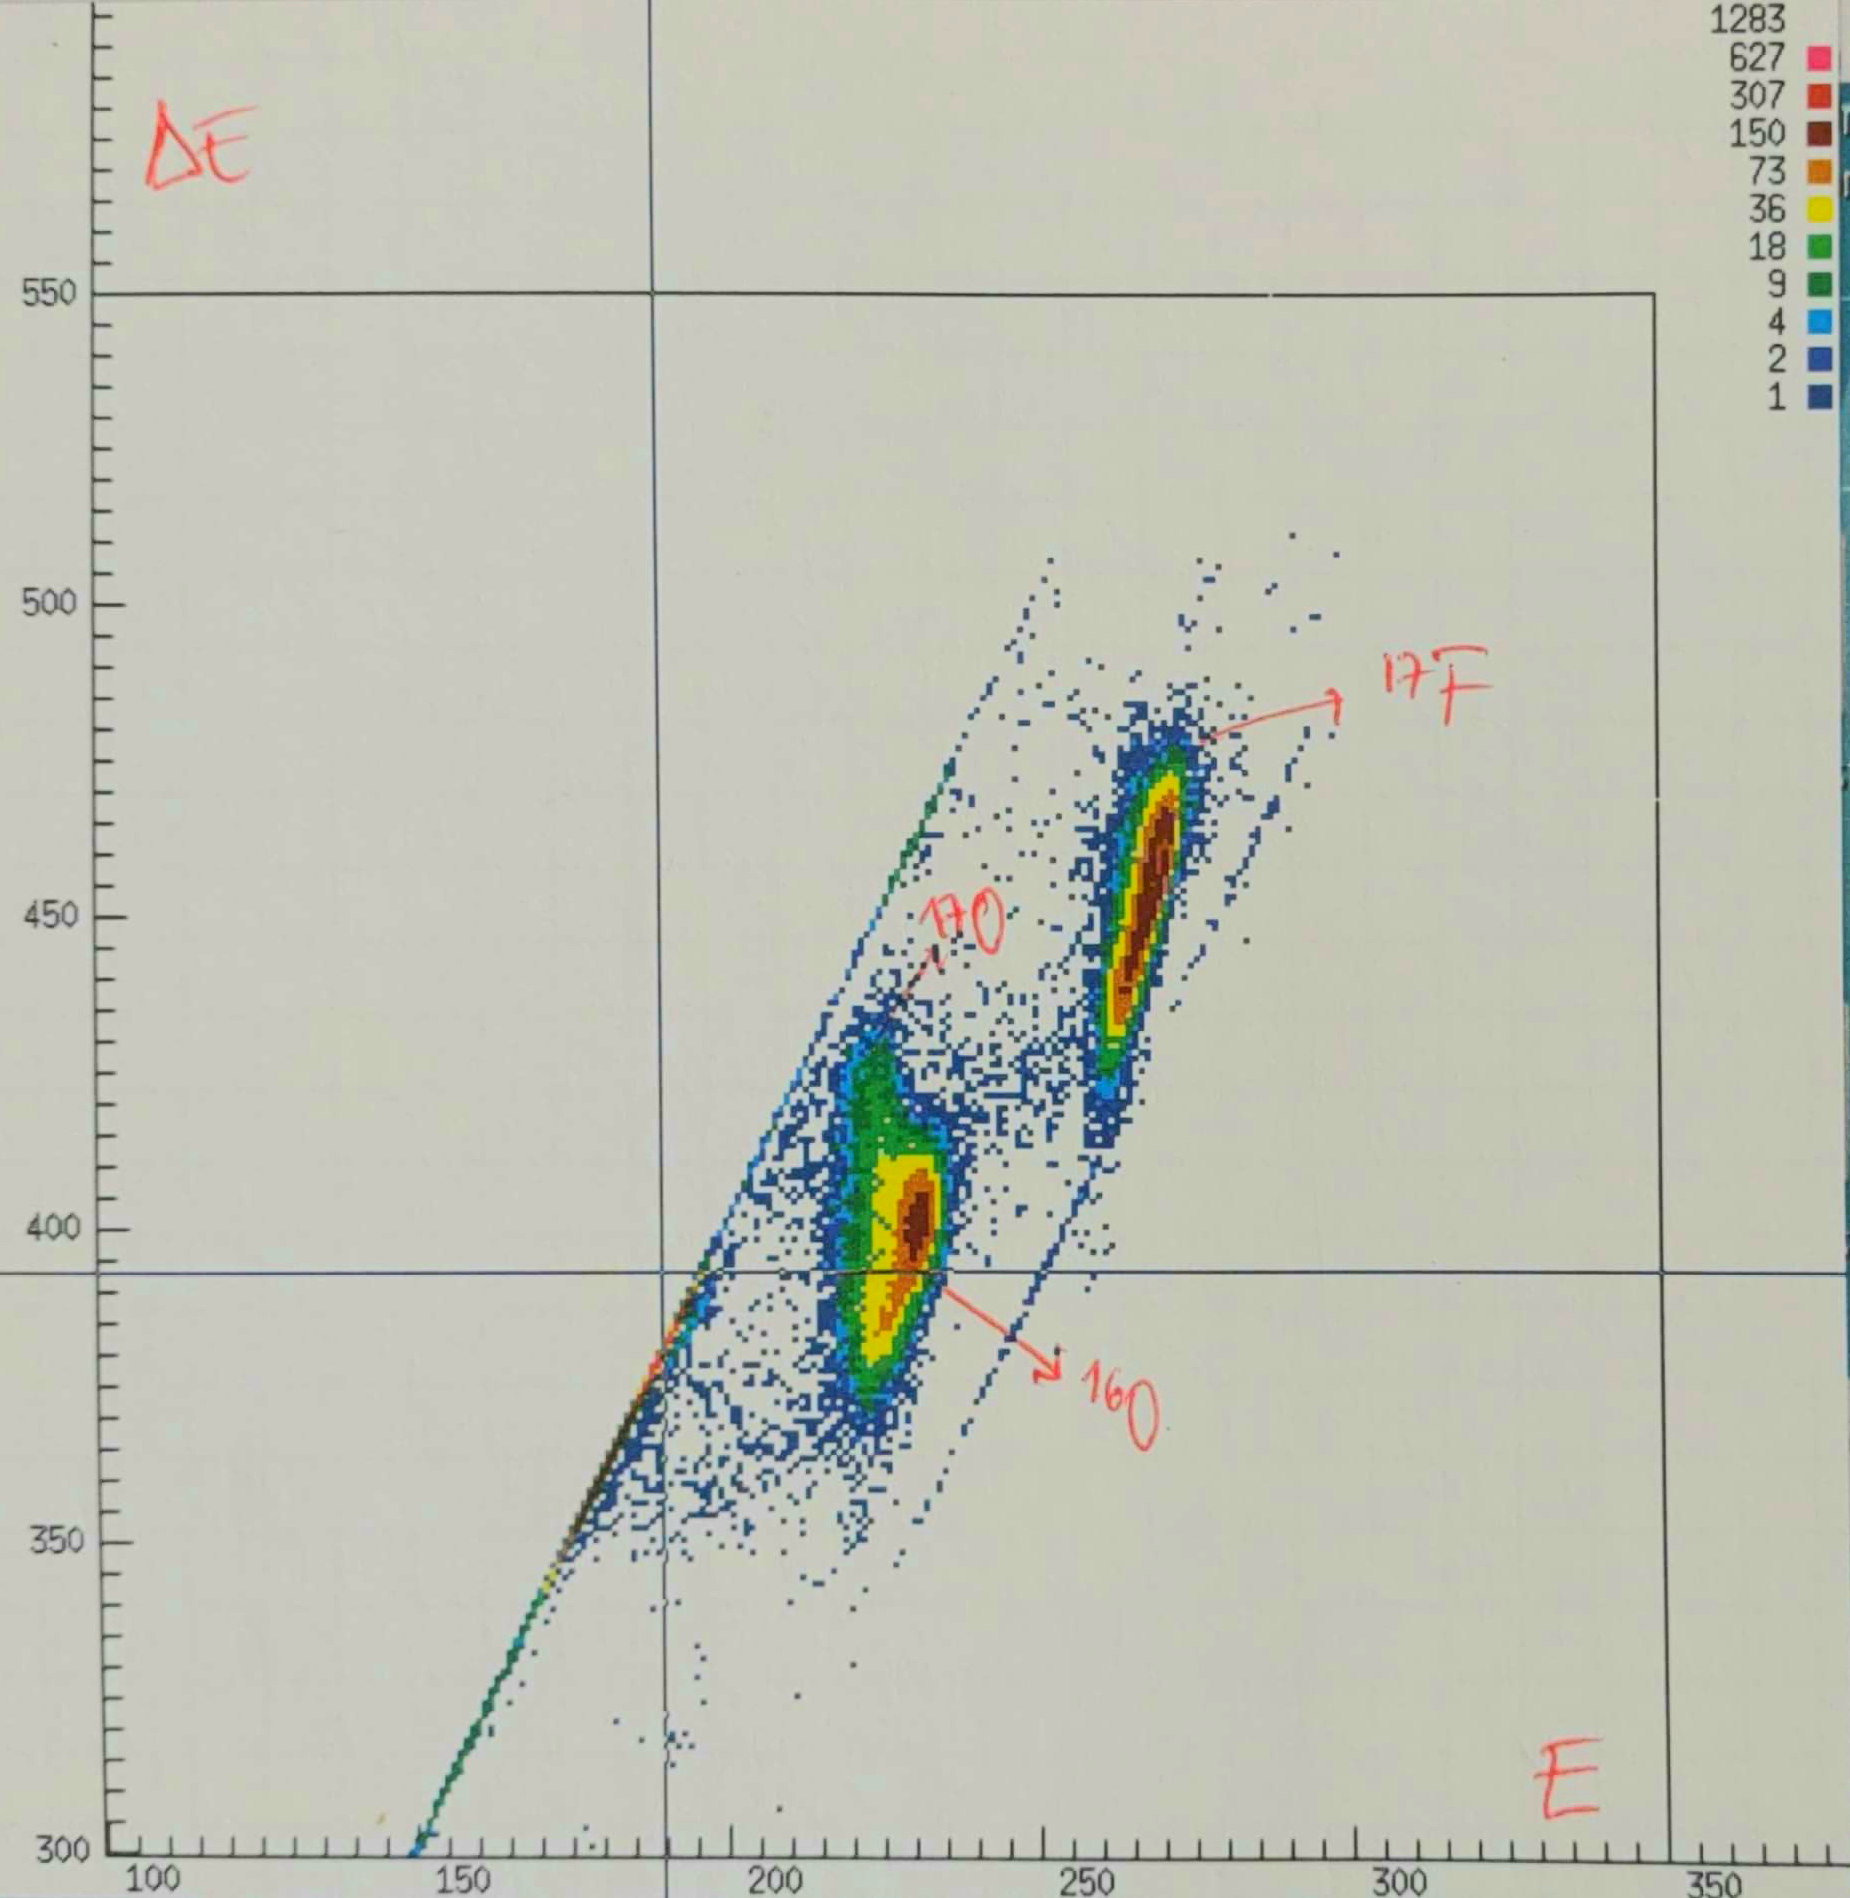
\includegraphics[scale = 0.12]{figs/pid_17F.png}
    \caption{Espectro biparamétrico $\Delta E$ - $E$ de identificação de partículas. Nele é possível identificar que o feixe possui a presença de $^{17}$F, $^{16}$O e uma pequena parte de $^{17}$O.}
    \label{fig:PID_17F}
\end{figure}

\par O alvo ativo será utilizado como detector e como alvo. A seguir está descrito o funcionamento desse equipamento.

\section{O alvo ativo pAT-TPC}

%\par Essa seção irá descrever brevemente propriedades geométricas e físicas relacionadas ao sistema de detecção usado neste experimento, o alvo ativo pAT-TPC.
%  O pAT-TPC é um detector preenchido com gás que é usado como alvo-ativo.

\par Alvos ativos vêm sendo cada vez mais utilizados em experimentos para investigações de reações nucleares \cite{FORTINO2022166497}, dentre os diversos laboratórios que utilizam alvos ativos podemos citar o TexAT \cite{KOSHCHIY2020163398} e o MAIKo \cite{FURUNO2018215}.

\par A figura \ref{subfig:pattpc} mostra o desenho esquemático do pAT-TPC, que possui o alvo ativo utilizado no experimento. O detector possui uma cela cilíndrica de 50 cm de comprimento e 28 cm de diâmetro, onde o seu eixo é alinhado com o eixo do feixe \cite{pattpc}, que passa pela câmara de íons até o duto central. Durante a passagem pela câmara de íons e pela janela (feita de PPTA com 12 $\mu m$ de espessura) do pATTPC, o feixe $^{17}$F perde energia e entra na câmara com cerca de 34.76 MeV. Nesse experimento, a câmara foi preenchida com $^4$He gasoso puro à uma pressão de 350 Torr que serve tanto para alvo de reações nucleares, quanto para a própria medição e detecção dos produtos da reação \cite{pattpc, pattpc2}. Tanto o feixe quanto partículas originadas da reação ionizam o gás e os elétrons que surgem dessa ionização foram conduzidos por um campo elétrico de 1 kV/cm perpendicular ao eixo da câmara até o plano detector (\textit{pad plane}), o \textit{Micromegas} \cite{micromegas}, mostrado na figura \ref{subfig:micromegas}.

\begin{figure}[H]
\centering
    \begin{subfigure}[t]{0.49\textwidth}
        \centering
        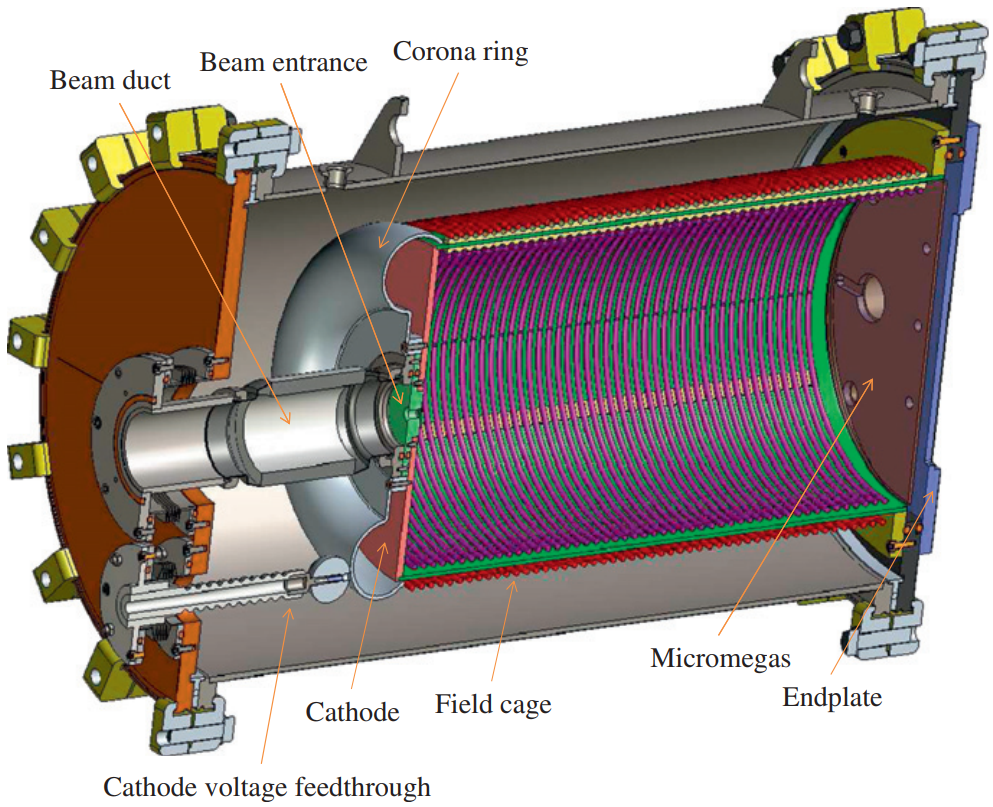
\includegraphics[scale=0.30]{figs/pattpc.png}
        \caption{Visão transversal do pAT-TPC. O gás é preenchido dentro da cela que possui um campo elétrico perpendicular ao plano do \textit{Micromegas}, à direita da figura. O feixe incide na câmara entrando pelo duto de feixe à esquerda da figura.}
        \label{subfig:pattpc}
    \end{subfigure}%
    \hfill
    \begin{subfigure}[t]{0.49\textwidth}
        \centering
        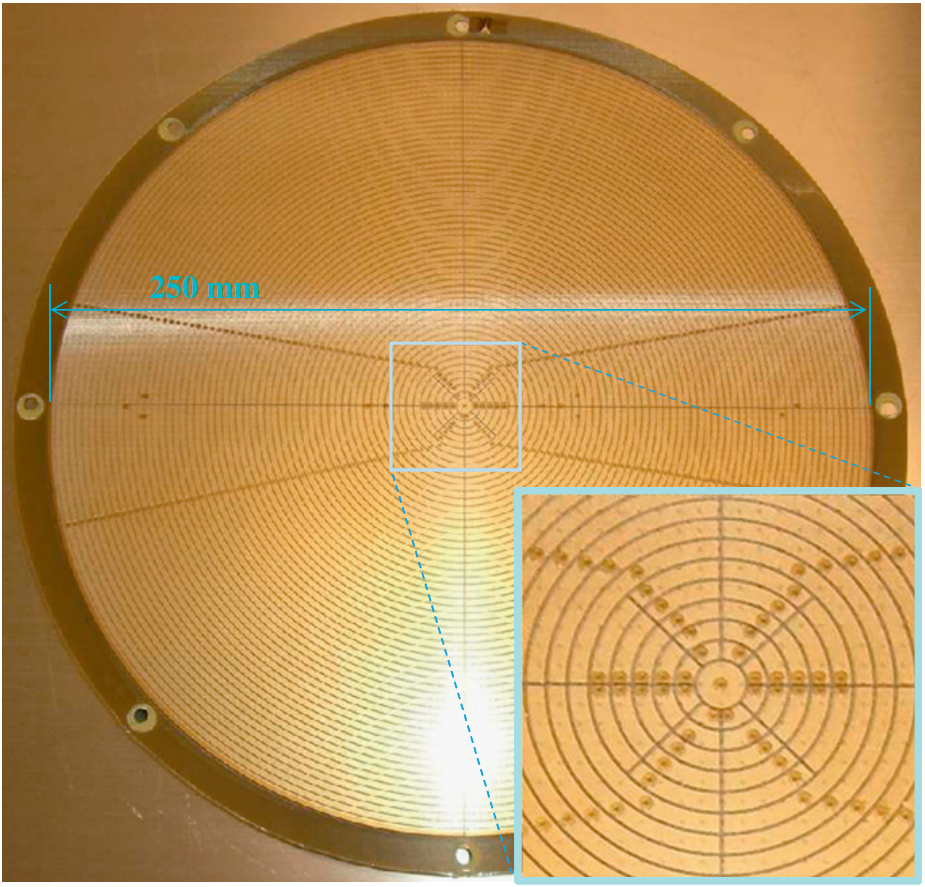
\includegraphics[scale=0.28]{figs/micromegas.png}
        \caption{Foto do \textit{Micromegas}. O detector é multipixelado com uma maior densidade no centro, parte destacada na imagem. O \textit{pad} central tem diâmetro de 5 mm enquanto que as faixas coaxiais possuem passo de 2mm \cite{attpc, josh_bradt}.}
        \label{subfig:micromegas} 
    \end{subfigure}
\caption{Figura esquemática do pAT-TPC e o detector \textit{Micromegas}\cite{pattpc}.}
\label{fig:pattpc_e_micromegas}
\end{figure}

\par O \textit{Micromegas} é um dispositivo de amplificação de elétrons, que consiste em um plano detector com 2048 canais (\textit{pads}) triangulares com eletrônica independente, que usa o \textit{Generic Electronics for TPCs} (GET) \cite{GET}. Detalhes sobre a eletrônica podem ser encontrados nas Refs. \cite{GET, josh_bradt}. O formato triangular dos canais tem como objetivo maximizar a resolução espacial do detector \cite{attpc}. Cada canal possui uma posição ($x$, $y$) fixa e a terceira coordenada $z$ será determinada a partir do tempo de deriva dos elétrons no gás \cite{pattpc, pattpc2, attpc, josh_bradt}. Isso só é possível pois a velocidade de deriva (\textit{drift}) dos elétrons é constante \cite{drift_constant}, portanto a posição em $z$ da partícula é diretamente proporcional ao tempo de voo. Esse princípio que deu origem ao nome de \textit{Time Projection Chamber}, pois o evento é projetado no tempo de deriva dos elétrons no gás. A equação  \ref{eq:langevin} (equação de Langevin) descreve o movimento de um elétron com massa $m$ e carga $e$ é descrito por \cite{drift_constant}

\begin{equation}\label{eq:langevin}
    m\frac{d\vec{v}}{dt} = e\left(\vec{E} +\vec{v}\times \vec{B}\right) - \frac{m}{\tau}\vec{v},
\end{equation}

onde $\vec{E}$ é o vetor campo elétrico, $\vec{B}$ o vetor campo magnético, $\vec{v}$ é o vetor de velocidade do elétron e $\tau$ é o tempo de colisão médio, que depende das propriedades termodinâmicas do gás. No caso deste experimento, $\vec{B}$ é zero e a solução estacionária para a velocidade de \textit{drift} do elétron é

\begin{equation}\label{eq:v_tpc}
    \vec{v} = \frac{\tau}{m}e\vec{E}.
\end{equation}

\par A velocidade de deriva depende das propriedades termodinâmicas do gás (temperatura, pressão) e também de sua condutividade elétrica \cite{drift_constant}. Isso significa que a calibração da velocidade não depende só do campo elétrico, mas também das propriedades do gás dentro do alvo ativo \cite{pattpc, drift_constant}. Para acharmos a coordenada $z$, basta integrar a equação \ref{eq:v_tpc} para obter

\begin{equation}
    z = \frac{\tau}{m}e\vec{E}(t - t_0),
\end{equation}

onde no tempo $t_0$ = 0 o elétron está no plano do detector ($z$ = 0).

\par O pAT-TPC conta com uma camada extra de \textit{thick gems} acoplada ao detector micromegas. \textit{Thick gems} usam do fato de que, no momento em que o elétron passa para uma região de campo elétrico ordens de grandeza maior que de sua origem, ocorre a ionização secundária (quando o elétron ioniza o gás). Isso provoca o que é chamado de avalanche de elétrons, amplificando a intensidade do sinal recebido \cite{GET}. A figura \ref{fig:thick_gems} mostra a esquematização do \textit{Micromegas}, onde na eletrônica de saída é produzido um sinal em função do tempo.

\begin{figure}[H]
    \centering
    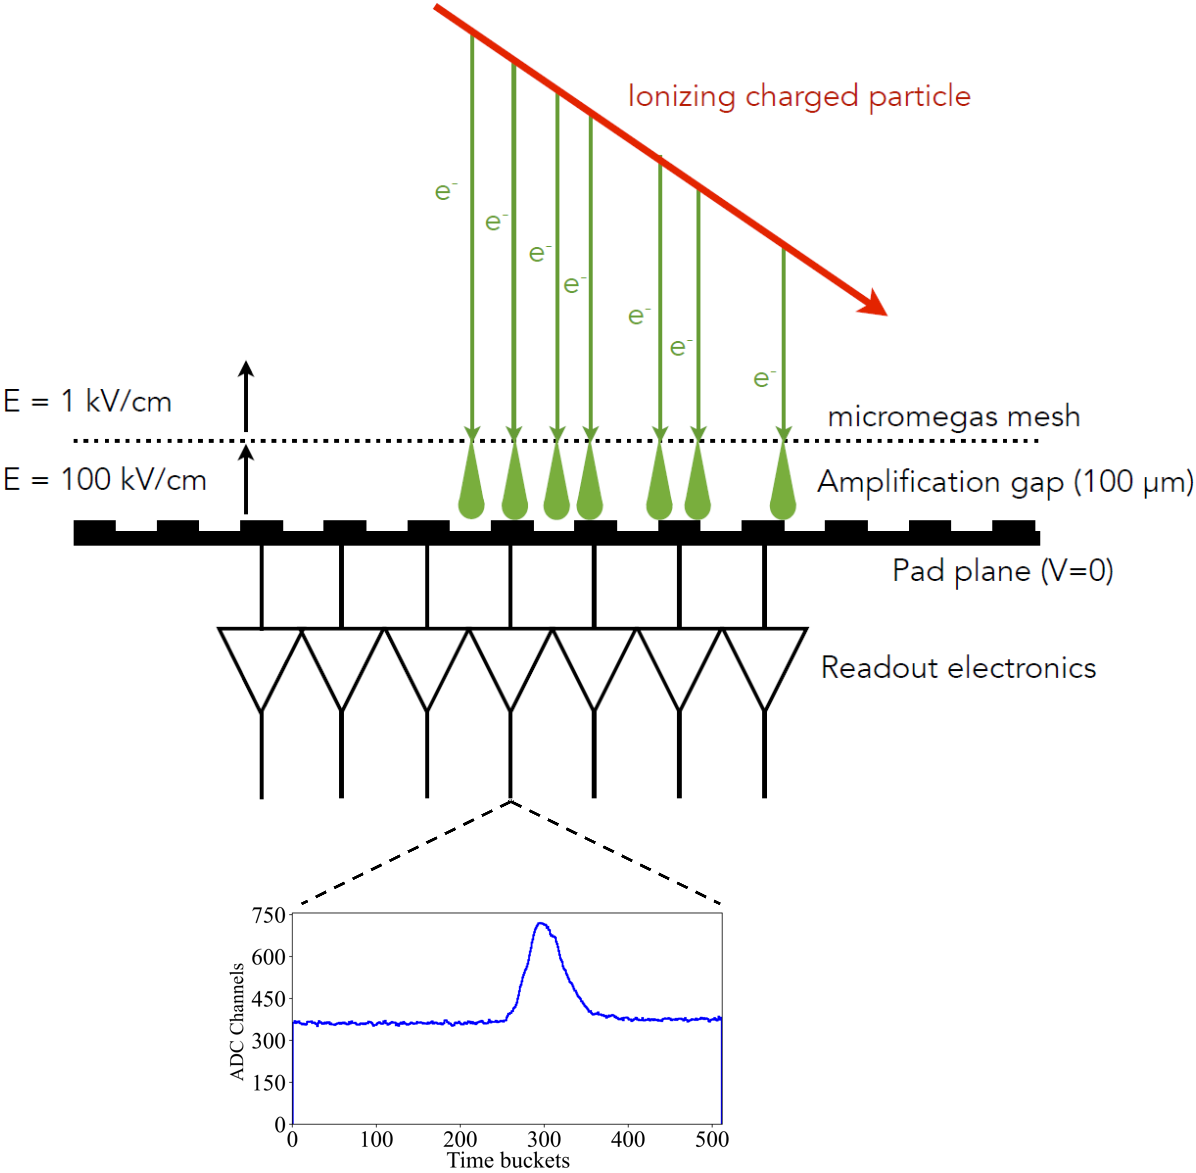
\includegraphics[scale = 0.40]{figs/thick_gems_2.png}
    \caption{Plano do \textit{Micromegas} com a esquematização das \textit{thick gems}. Os elétrons quando passam para um campo elétrico mais intenso ionizam o gás, produzindo ainda mais elétrons (evento chamado de avalanche de elétrons). Cada canal da eletrônica de saída produz um pulso como mostrado na parte de baixo da figura.}
    \label{fig:thick_gems}
\end{figure}

\par O sinal é discretizado no tempo levando em conta a velocidade de deriva dos elétrons, dividindo em 512 canais o tempo que o elétron leva para percorrer toda câmara do TPC \cite{josh_bradt, pattpc}. A velocidade de deriva do elétron no gás $^4$He é da ordem de 5 $mm$/$\mu s$  \cite{pattpc}, onde o elétron percorre os 50 cm da câmara em cerca de 100 $\mu s$. Dividindo esse tempo pelos 512 canais tem-se que cada canal (\textit{time bucket}) possui 192 $ns$ de largura. Cada centroide identificado é um ponto de interação de uma partícula carregada com o gás. A carga acumulada $Q$ dessa interação é a área do pulso associado ao centroide. Cada centroide então representa um ponto no espaço ($x$, $y$, $t$, $Q$). Um exemplo de evento reconstruído está na figura \ref{fig:event_cap_exp}.

\begin{figure}[H]
    \centering
    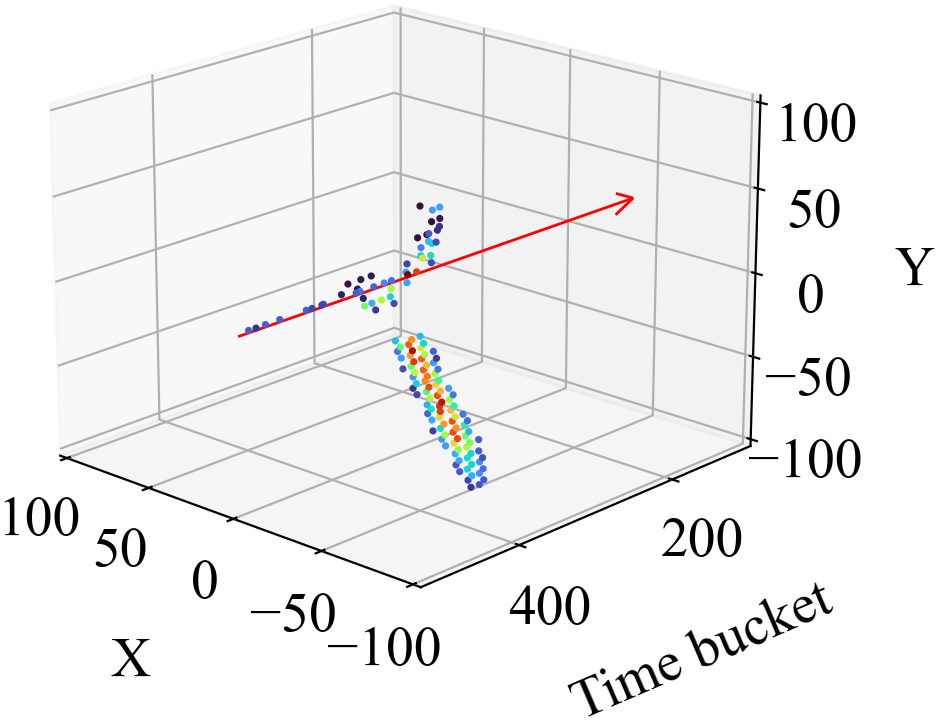
\includegraphics[scale = 0.40]{figs/event_cap_exp.png}
    \caption{Evento reconstruído a partir da análise dos pulsos gerados pelo \textit{Micromegas}. A cor representa a carga integrada de cada ponto de interação com o gás.}
    \label{fig:event_cap_exp}
\end{figure}

\par Para reconstituir eventos como o da figura \ref{fig:event_cap_exp}, foram analisados cerca de 300 pulsos. Existem canais auxiliares que servem para evitar armazenar canais sem detecção. Caso haja detecção além do centro do \textit{Micromegas} então os sinais gerados pelo evento são armazenados \cite{josh_bradt, attpc}. O número de eventos reconstruídos é da ordem de milhões, portanto a quantidade de sinais que precisam ser analisados é muito grande, em comparação com experimentos em física nuclear com apenas alguns canais de detecção, o que gera a necessidade de desenvolvimento de algoritmos extremamente eficientes em tempo para que a análise não demande muito tempo. Para a análise completa do experimento foram seguidas as seguintes etapas:

% \par Nem todos os \textit{pads} do detector são ativados por evento. Existem canais auxiliares que servem para evitar armazenar canais sem detecção. Caso haja detecção além do centro do \textit{Micromegas} então os sinais gerados pelo evento são armazenados\cite{josh_bradt, attpc}. São gerados cerca de 300 sinais por evento, sendo que existem milhões de eventos, o que gera a necessidade de desenvolvimento de algoritmos extremamente eficientes em tempo para a análise. Para a análise completa do experimento precisamos seguir as seguintes etapas:

\begin{itemize}
    \item Análise dos pulsos de cada interação das partículas com o gás. Isso envolve remover o fundo, localizar os picos e obter os tempos e carga integrada de cada caso;
    \item Reconstruir eventos em 3D (nuvens de pontos) a partir da análise de sinais. As nuvens de pontos precisam ser analisadas com algoritmos de reconhecimento de padrões que permitem ajustar as trajetórias das partículas em 3D;
    \item Reconstruir a cinemática das partículas com as trajetórias e energia depositada no gás. Isto permite obter as distribuições angulares. 
\end{itemize}

% \begin{itemize}
%     \item Reconstruir os eventos tridimensionais (nuvens de pontos) a partir dos sinais gerados pelo \textit{micromegas}. Isso inclui remover o fundo, localizar todos os pontos de interação das partículas carregadas com o gás etc. Isso será mostrado em detalhes no capítulo \ref{chapter:sinais};
%     \item A partir das nuvens de pontos é necessário reconstruir a cinemática das reações, identificando trajetórias das partículas e o vértice de reação;
%     \item Com a cinemática reconstruída podemos associar as partículas com as trajetórias e finalmente construir as seções de choque. 
% \end{itemize}

\par A análise dos pulsos, reconstituição de eventos, reconstrução da cinemática, gráficos das distribuições angulares e resultados são apresentadas nos próximos capítulos.

% \chapter{Uma breve introdução ao \textit{Machine Learning}}\label{sec:ml}
\chapter{Desenvolvimento de ferramentas de \textit{machine learning} para analise de dados}\label{sec:ml}

\par Para que possamos analisar a grande quantidade de dados gerados em experimentos com alvo ativo podemos utilizar técnicas de \textit{machine learning}. Nesse capítulo está explicada a metodologia usada para a implementação dessas ferramentas. O apêndice \ref{appendix:ml_nuclear} mostra algumas aplicações de \textit{machine learning} na física nuclear.

\par \textit{Machine learning} é a área de estudo que desenvolve algoritmos para que eles possam aprender com os dados, sem serem explicitamente programados para isso \cite{mlbook}. Supõe-se que uma rede neural imite um sistema biológico, em que os neurônios interajam enviando sinais na forma de funções matemáticas entre as camadas. Isso inspirou o uso do modelo matemático simples de uma função linear nos parâmetros para um neurônio artificial \cite{curso}:

\begin{equation}\label{eq:model_n}
    y = f\left(\sum^{n}_{i = 1}\omega_i x_i + bi\right) = f(z),
\end{equation}

\par onde $y$ é a saída do neurônio, que corresponde à função de ativação $f$ que depende da soma ponderada, onde o peso é $\omega_i$, das entradas $x_i$ dos outros $n$ neurônios. O termo $b_i$ corresponde ao parâmetro \textit{bias}. A ideia é fazer um neurônio receber a informação de todos os outros neurônios da camada anterior, fazendo uma média ponderada (onde o peso que será estimado pelo algoritmo de \textit{machine learning}) e somando com um termo independente (\textit{bias}, que também é estimado). Os parâmetros $\omega_i$ e $b_i$ serão estimados através de um determinado procedimento, chamado de minimização (o treino da rede neural).

\section{Tipos de redes neurais}

\par Uma rede neural artificial, \textit{Artificial Neural Network} (ANN), é um modelo computacional que consiste de camadas de neurônios. ANNs foram desenvolvidas para o estudo de inteligência artificial\cite{mlbook, mldiverso}. ANNs consistem principalmente numa camada de entrada (\textit{input layer}), uma camada de saída (\textit{output layer}) e eventuais camadas entre essas duas, chamadas de camadas ocultas (\textit{hidden layers}). Os tipos mais comuns são:

\subsubsection*{Feed-Forward Neural Networks}

\par A \textit{Feed-forward neural networks} (FFNN) é a primeira e mais simples rede neural desenvolvida \cite{talent_ml, bishop2016pattern}. Nessa rede a informação se move apenas para frente através de camadas (da camada de entrada até a camada de saída). A figura \ref{fig:FFNN} mostra uma representação de rede, onde os neurônios são representados por círculos, enquanto que as linhas mostram as conexões entre os neurônios. Cada neurônio recebe informação de todos os neurônios da camada anterior, portanto a rede é chamada de totalmente conectada, \textit{fully-connected} (FC), FFNN. 

\begin{figure}[H]
    \centering
    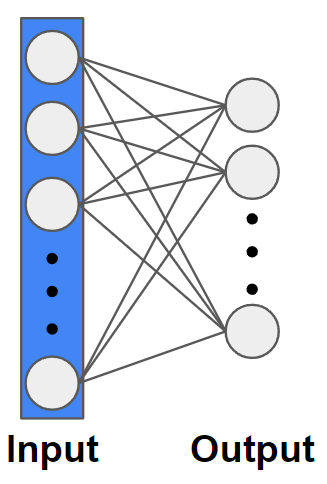
\includegraphics[scale = 0.55]{figs/FFNN.png}
    \caption{Exemplo de FFNN. A camada de entrada na esquerda propaga a informação para a direita (camada de saída). Todos os neurônios entre camadas estão conectados entre si.}
    \label{fig:FFNN}
\end{figure}

\subsubsection*{Convolutional Neural Network}

\par Uma variante da FFNN é a chamada de rede neural convolucional, \textit{convolutional neural network} (CNN). Do ponto de vista matemático sobre convoluções, a convolução descrita como $(f*g)(t)$ de uma função $f(t)$ e outra $g(t)$ é definida como:

\begin{equation}\label{eq:conv_cont}
    (f*g)(t) \equiv \int^{\infty}_{\infty} f(\tau)g(t - \tau)d\tau.
\end{equation}

Para o caso discreto, com $g$ sendo uma função resposta finita de tamanho $2M$, temos

\begin{equation}\label{eq:conv_disc}
    (f*g)[n] = \sum^{M}_{m = -M} f[n - m]g[m]. 
\end{equation}

\par Convoluções são invariantes sobre rotação e translação, portanto são muito utilizadas para processamento de sinais e imagens \cite{signal_book}. Para a convolução discreta se escolhe um filtro que irá atuar no vetor desejado. Para ilustrar o que significa isso, no caso discreto e unidimensional, a figura \ref{fig:conv_valid} mostra o processo de convolução de um vetor de tamanho 9 e um filtro de tamanho 3.

\begin{figure}[H]
    \centering
    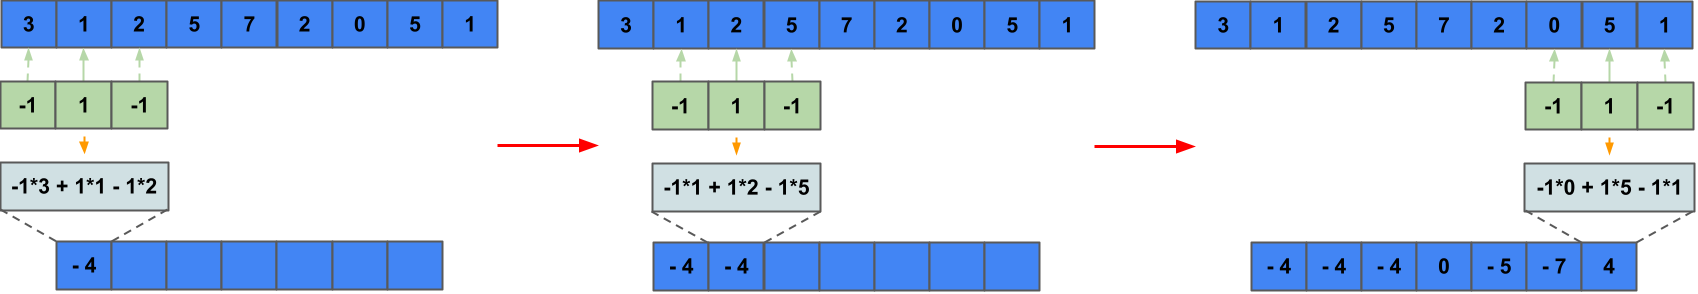
\includegraphics[scale = 0.38]{figs/conv_valid.png}
    \caption{Processo de convolução entre sinal azul em cima e o filtro em verde, resultando no sinal azul embaixo. A multiplicação é feita ponto a ponto e está indicada na caixa azul-clara.}
    \label{fig:conv_valid}
\end{figure}

\par Percebe-se que o sinal resultante tem dimensão menor que o sinal original. O filtro (também chamado de \textit{kernel}) atua em um ponto que possua vizinhos o suficiente para o restante do filtro poder fazer a multiplicação ponto a ponto. Esse tipo de convolução tem o chamado emparelhamento válido (\textit{valid padding}). O tamanho $n_2$ resultante do vetor de saída é 
\begin{equation}
    n_2 = n_1 - m + 1,
\end{equation}

\par onde $n_1$ é o tamanho do vetor de entrada e $m$ o tamanho do filtro (\textit{kernel size}). Para que o vetor de saída tenha o mesmo tamanho do vetor de entrada, são acrescentados zeros em torno da entrada, de forma que a saída tenha o mesmo tamanho da entrada. Esse é o chamado emparelhamento igual (\textit{same padding}). A figura \ref{fig:conv_same} ilustra esse processo.

\begin{figure}[H]
    \centering
    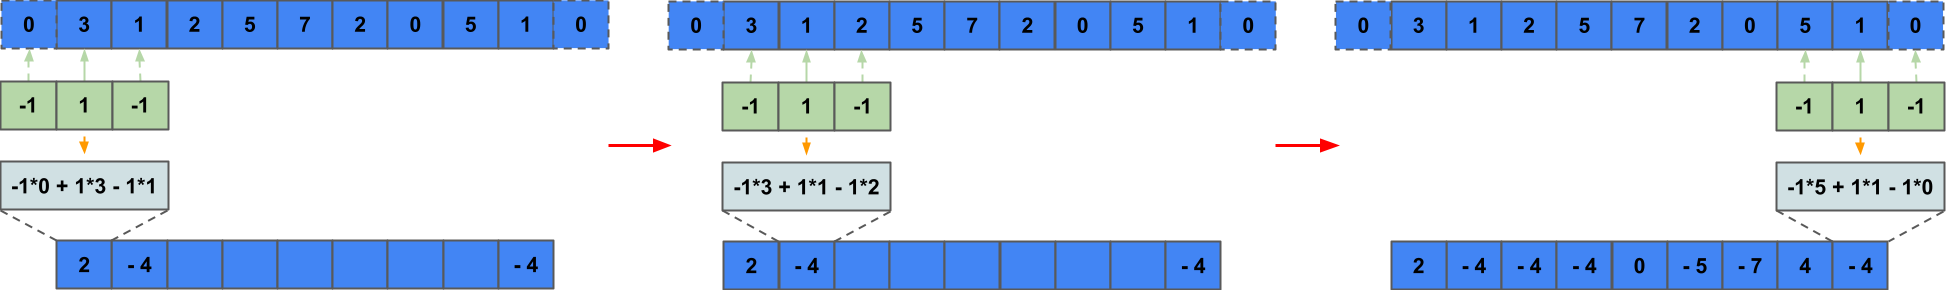
\includegraphics[scale = 0.38]{figs/conv_same.png}
    \caption{Processo de convolução entre o sinal azul em cima e o filtro em verde, resultando no sinal azul embaixo. Agora são acrescentados zeros no inicio e no final do vetor para que o vetor saída tenha o mesmo tamanho do vetor de entrada (nesse caso 9).}
    \label{fig:conv_same}
\end{figure}
%Uma CNN é capaz de fazer convoluções.
\par Como estamos no contexto de \textit{machine learning} (inteligência artificial), \textit{a priori} não sabemos quais os valores dos filtros que devem ser aplicados, apenas seus tamanhos e como agem. A ideia é estimar os valores do filtro (através do treino da rede neural) que deve ser aplicado para se obter o resultado desejado.

\par Cada filtro aplicado gera um mapa característico (\textit{feature map}), que é o resultado da atuação do filtro em um vetor. Usualmente, em uma CNN se escolhe o tamanho do filtro, \textit{padding} (\textit{valid} ou \textit{same}) e quantos filtros serão aplicados (para saber quantos \textit{feature maps} serão gerados). Como temos vários mapas gerados por cada filtro, isso acarreta em um aumento de dimensionalidade. Para filtrar/selecionar os mapas é usado um critério, como por exemplo selecionar valores máximos dos mapas gerados dada uma janela de atuação (quantos mapas serão comparados para selecionar o máximo valor). O \textit{Max-Pooling} faz isso, selecionando valores máximos para uma determinada quantidade de mapas sendo comparados (\textit{pool size}).

% Os filtros têm seus valores estimados pelo treino da rede neural, gerando vários mapas (\textit{feature maps}).

\par Existem outros tipos de redes neurais que não estão discutidas aqui, porém podem ser encontradas nas referências \cite{rbfbook, RNN_fund}.

\section{Estrutura da rede neural}

\par Para a construção de uma rede neural (nesse caso em específico de uma rede neural supervisionada, que está discutida mais para frente), é preciso definir sua estrutura. A estrutura da rede neural possui camadas e cada camada pode possuir uma função de ativação. No geral, tanto o \textit{input} quanto o \textit{output} possuem dimensão fixa. A rede é treinada minimizando uma função custo, otimizando os parâmetros da rede através de um otimizador.

%\par Para a construção de uma rede neural , precisamos primeiro entender sobre os dados que estamos trabalhando. Grande parte das redes neurais possuem um \textit{input} que deve ter dimensão fixa. O mesmo vale para o \textit{output}.

\par Para cada camada da arquitetura devemos escolher sua função de ativação. Tanto FNNNs quanto CNNs podem possuir funções de ativação (função $f$ da equação \ref{eq:model_n}). Dentre muitas funções de ativação podemos citar a \textit{Rectified Linear Units} (ReLU)\cite{RELU}, sigmoide \cite{sigmoid_act}, linear e tangente hiperbólica\cite{act_comp}. A figura \ref{fig:ativacoes} mostra os gráficos dessas funções de ativação, onde no eixo x é o argumento e no eixo y o resultado da função.

\begin{figure}[H]
    \centering
    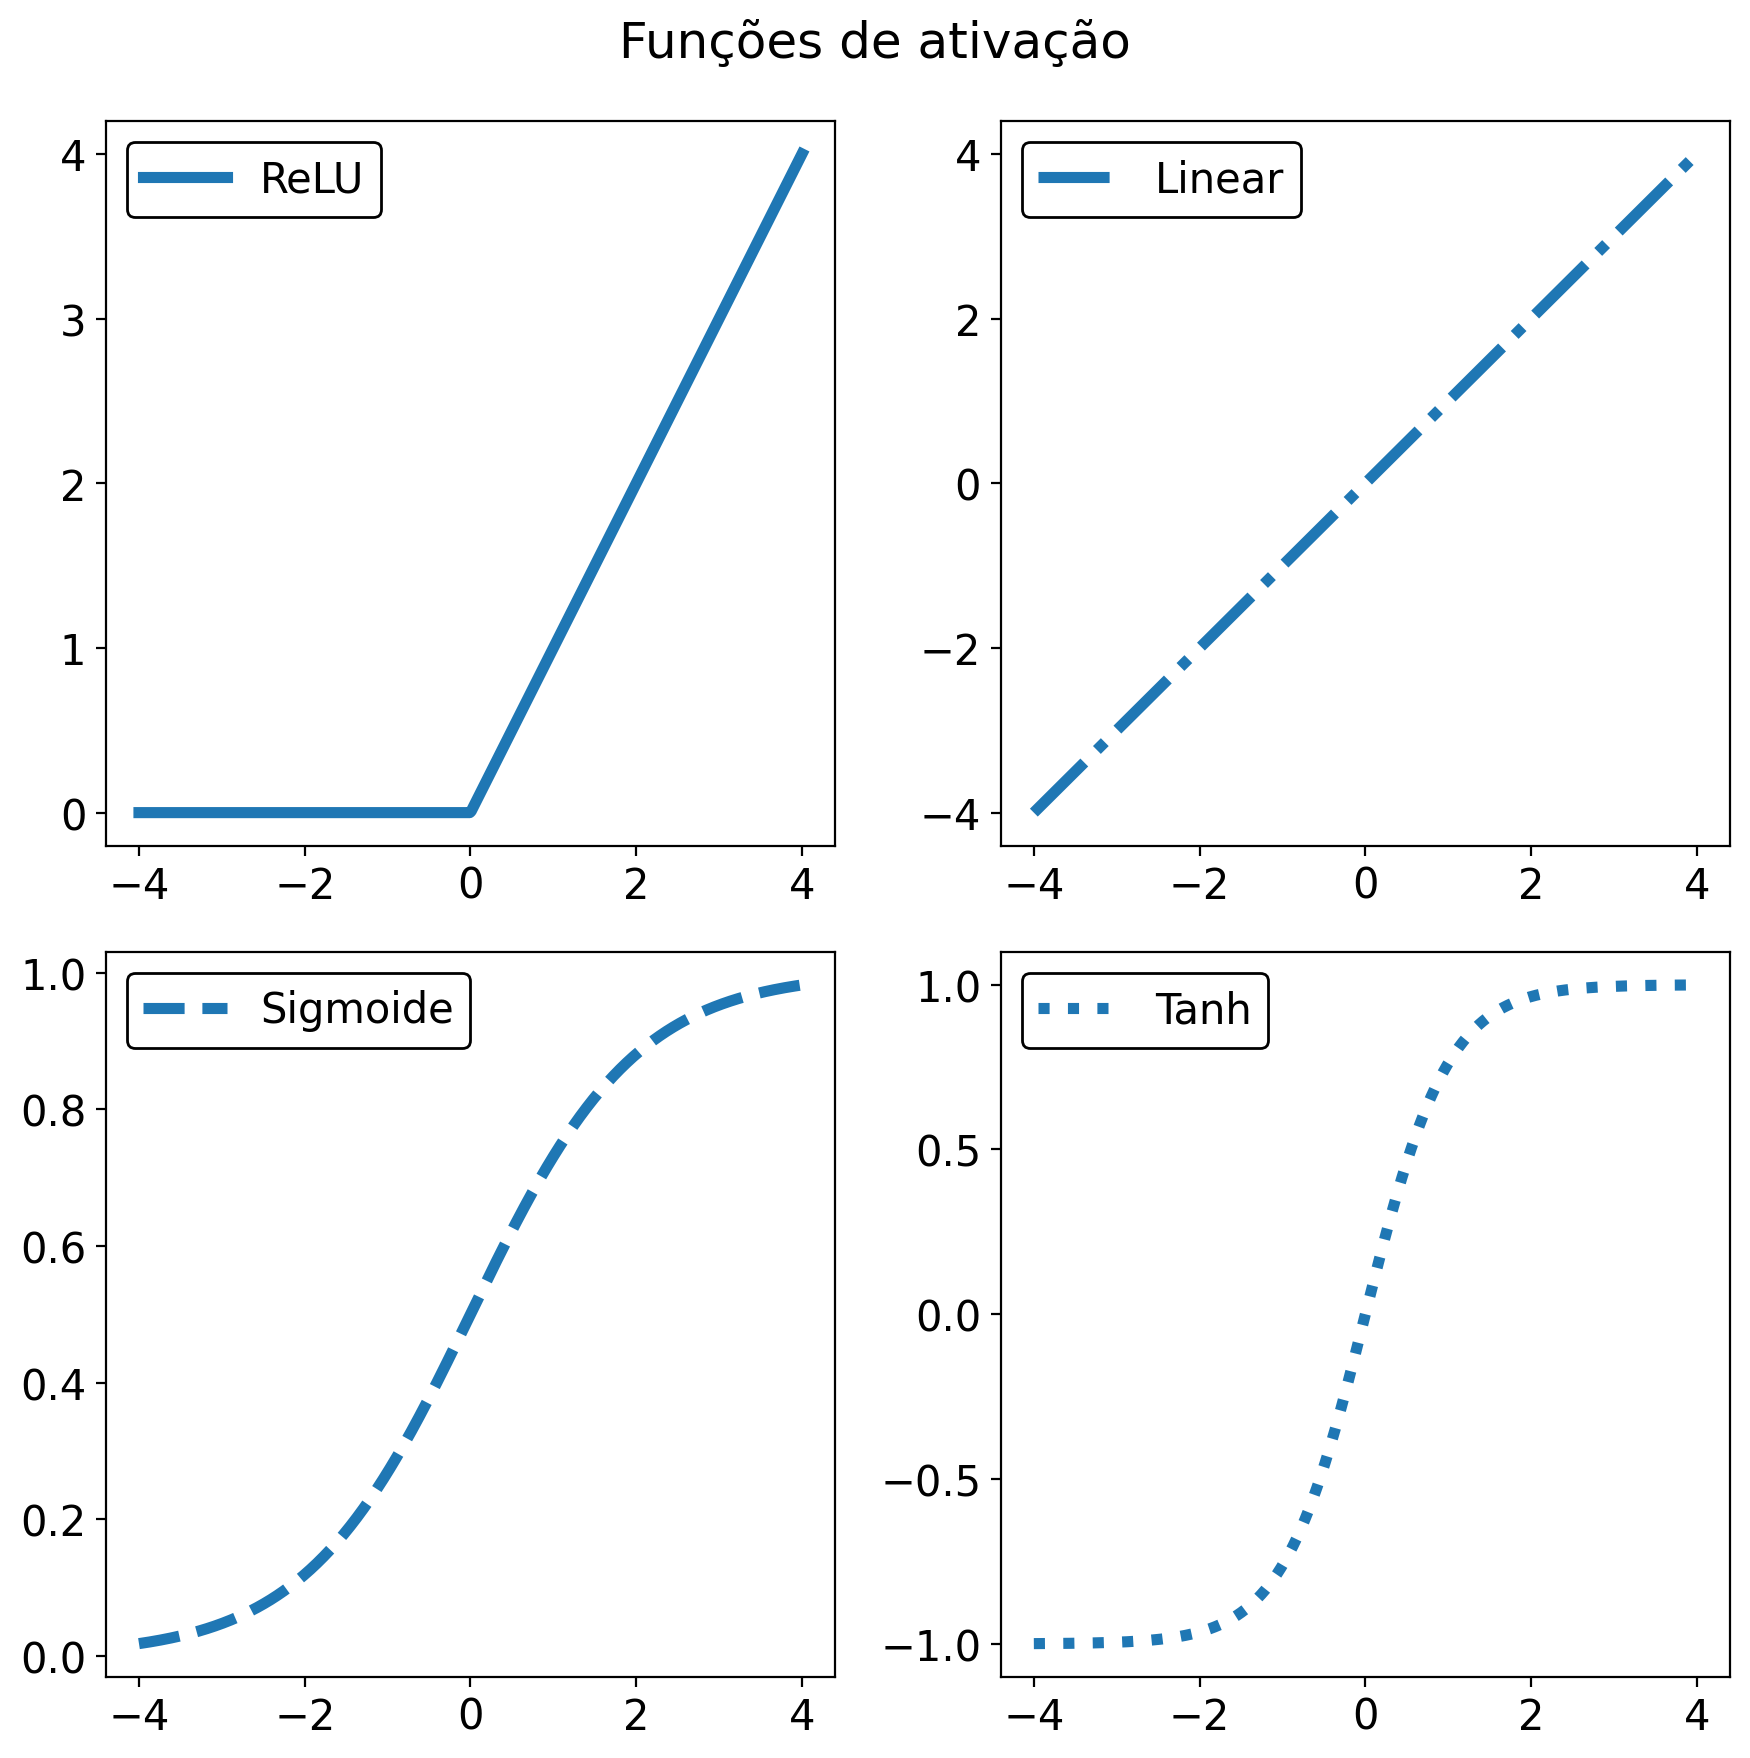
\includegraphics[scale = 0.7]{figs/ativacoes.png}
    \caption{Funções de ativação e seus respectivos gráficos.}
    \label{fig:ativacoes}
\end{figure}

\par O próximo passo é definir a função custo (também chamada de \textit{loss}) e o otimizador. A função custo tem o papel de retornar valores altos para previsões erradas e valores baixos para previsões corretas. Por exemplo, se queremos treinar uma rede neural para classificação binária (que prevê duas saídas possíveis), devemos usar a função custo chamada de \textit{binary cross-entropy} dada por\cite{dl_book}

\begin{equation}\label{eq:binary_cross_entropy}
    C(p(y_i)) = -\frac{1}{N}\sum_{i = 1} ^N y_i \log(p(y_i)) + (1 - y_i)\log(1 - p(y_i)),
\end{equation}

\par onde $y_i$ é o rótulo (\textit{label}), $p(y_i)$ é a probabilidade do ponto $y_i$ ser 1 e $N$ é o número de pontos. O objetivo da rede neural é achar o mínimo da função $C(p(y_i))$, o que implica diretamente na melhor solução para o conjunto de dados. Isso é feito pelo método de retropropagação do erro (\textit{backpropagation} \cite{backpropagation}) por um otimizador. Outros exemplos de \textit{loss} são o erro quadrático médio ou \textit{categorical cross-entropy} \cite{MSE_CEF_review}.

\par O otimizador tem o objetivo de otimizar os parâmetros presentes na rede neural, buscando o mínimo global da função custo, o que nem sempre acontece, pois a minimização pode parar em um mínimo local da função. Existem diversos otimizadores, como por exemplo o \textit{Stochastic Gradient Descent} (SGD), ADAM, ADAMAX \cite{ADAMAX}, entre outros \cite{gradient_over}. Para o SGD, temos que a atualização de parâmetros é dada por

\begin{equation}\label{eq:SGD}
    \theta_j = \theta_{j} - \alpha \frac{\partial }{\partial \theta_j}C(\theta),
\end{equation}

\par onde $\theta_j$ é o parâmetro a ser atualizado, $\alpha$ é a \textit{learning rate} e $C(\theta)$ é a \textit{loss} que depende dos parâmetros $\theta$.

\par Para enfim treinar a rede neural, se escolhe o \textit{batch size}, que é o tamanho de amostras que será usada para o treino, por iteração em cada rodada de treino (\textit{epoch}). Por exemplo, se usamos 1000 dados para o treino, e o \textit{batch size} é 500, cada \textit{epoch} terá duas iterações. No geral, se usam \textit{batch sizes} pequenos, pois o consumo de memória é mais eficiente.

\par Para avaliação do modelo se usam dados de validação, que servem para verificar o comportamento da rede neural que está sendo treinada. Esse conjunto de dados usados não é usado para o treino, são usados apenas para verificar possíveis problemas como o \textit{overfit}. O \textit{overfit} ocorre quando a rede neural começa a se adequar perfeitamente aos dados de treino, perdendo a capacidade de previsão em dados que não estão sendo usados no treino pela rede neural.

\par Além dos dados de validação, podemos escolher métricas que auxiliam a visualização do comportamento da rede neural durante o treino e nos retornam informações importantes sobre sua qualidade. Exemplos importantes de métricas são: acurácia binária, erro médio absoluto e acurácia categórica \cite{metrics}. Por exemplo, caso seja necessário verificar se uma rede neural está fazendo previsões certas em um problema cuja classificação é binária, então a métrica deve ser a acurácia binária. Tudo depende do objetivo da rede neural.

\section{Sistemas de \textit{machine learning}}

Podemos dividir os sistemas de \textit{machine learning} em quatro tipos:

\subsubsection*{Aprendizado Supervisionado}
% \begin{enumerate}
%     \item aprendizado supervisionado;
%     \item aprendizado não supervisionado;
%     \item aprendizado semi supervisionado;
%     \item aprendizado por reforço.
% \end{enumerate}

\par Aprendizado supervisionado é quando fornecemos para a rede neural um conjunto de dados para o treino com a solução desejada (chamados de \textit{labels}). Um uso típico é para problemas de classificação \cite{mlbook}. Por exemplo, classificação de imagens (identificação de figuras), previsão de valores numéricos etc. Exemplos de de algoritmos supervisionados são:

\begin{itemize}
    \item \textit{k-Nearest Neighbors} \cite{knn}
    \item Regressão linear
    \item \textit{Support Vector Machines} (SVMs)
    \item \textit{Decision Trees} and \textit{Random Forests}
    \item Redes neurais
\end{itemize}

\subsubsection*{Aprendizado não supervisionado}

\par Aprendizado não supervisionado é quando fornecemos o conjunto de dados para o treino, porém sem solução. A ideia é aprender sem supervisão. Um problema comum, por exemplo, é quando queremos identificar \textit{clusters} em um conjunto de dados (\textit{clustering})  \cite{unsupervised, knn_uns}.

\subsubsection*{Aprendizado semi supervisionado}

\par Aprendizado supervisionado é quando apenas parte do conjunto de dados para o treino possui \textit{labels}. Isso é comum quando se obtém conjuntos de dados diferentes e apenas parte deles foi classificado \cite{semi_supervised}.

\subsubsection*{Aprendizado por reforço}

\par Aprendizado por reforço é quando um sistema, chamado de \textit{agente} nesse contexto, aprende através do ambiente, realizando ações que maximizam sua recompensa. Por exemplo, caso o sistema realize uma ação incorreta, ele recebe uma penalidade, fazendo com que procure outra maneira de realizar a ação, dessa vez de maneira correta, para poder ganhar uma recompensa \cite{reinforcement}. Esse tipo de sistema é muito usado, por exemplo, em automatização robótica, como carros que pilotam sozinhos, robôs que aprendem a andar etc \cite{robot_ml}.

%\section{Aplicações de \textit{machine learning} na física nuclear}


\par Com essa breve descrição sobre \textit{machine learning} e exemplos do seu uso em problemas de física nuclear (apêndica \ref{appendix:ml_nuclear}), pode-se seguir adiante e entender seu uso dentro deste trabalho, que está feito nos próximos capítulos.

\chapter{Reconstrução de nuvens de pontos a partir de algoritmos de \textit{machine learning}}\label{chapter:sinais}

\par Esse capítulo descreve o procedimento usado para criar as nuvens de pontos (\textit{pointclouds}) a partir dos pulsos gerados por cada pixel do \textit{micromegas}, usando algoritmos de \textit{machine learning} supervisionado.

\par Algoritmos baseados em CNNs vem sendo usados com relativo sucesso para o processamento e análise de sinais \cite{FORTINO2022166497}, como por exemplo para discriminação de pulsos \cite{Holl2019}. CNNs possuem a capacidade de fazer ajustes multidimensionais e aprender padrões complexos. Além disso, CNNs são mais eficientes em tempo para a análise de grandes quantidades de dados em comparação com algoritmos comuns \cite{FORTINO2022166497}.

\par A quantidade de pulsos gerados nesse experimento é da ordem de centenas de milhões. Para a análise completa dos pulsos, são necessárias diferentes etapas que envolvem processos que muitas vezes precisam ser refeitos por causa de algum um erro no processo análise. Notar algum erro no processo, ou ter que mudar algum parâmetro da análise, significaria ter que analisar novamente os dados, sendo um processo muito custoso em tempo.

\par O uso de algoritmos de CNNs tem o objetivo de diminuir o tempo consumido para a análise dos pulsos. As redes neurais criadas são treinadas uma única vez e podem ser utilizadas de modo separado e/ou acoplado \cite{FORTINO2022166497}, como está mostrado na sequencia do capítulo.

\par A análise dos dados experimentais foi dividida em três etapas: correção do fundo, deconvolução do sinal e identificação de picos. As redes neurais criadas foram supervisionadas, o que significa que foi preciso determinar a entrada (\textit{input}) e a saída (\textit{output}) das redes. Para isso foi feito um grande banco de dados, para utilizar no treinamento das redes neurais, que se beneficiam da grande quantidade de dados usada para o treino \cite{mlbook}.

\par Na seção \ref{sec:pulses_trad}, está mostrado como o banco de dados para o treino das redes neurais desenvolvidas foi criado, e a construção das redes neurais está na seção \ref{sec:pulsos_ml}.


% os sinais foram analisados a partir de métodos mais tradicionais e depois criando algoritmos de \textit{machine learning}, usando das soluções anteriores como base para o seu funcionamento.


% \par A quantidade de histogramas armazenados ultrapassa facilmente a casa das centenas de milhões, portanto é necessário o desenvolvimento de algoritmos extremamente rápidos para a análise.


\section{Construção do banco de dados para as redes neurais}\label{sec:pulses_trad}

\par Cada um dos pixels do detector micromegas possui uma eletrônica independente que gera pulso digitais como os mostrados na \ref{fig:exemplos_sinais}. Centenas de sinais coo essas são produzidas em cada um dos eventos.

\begin{figure}[H]
\centering
    \begin{subfigure}[b]{0.48\textwidth}
        \centering
        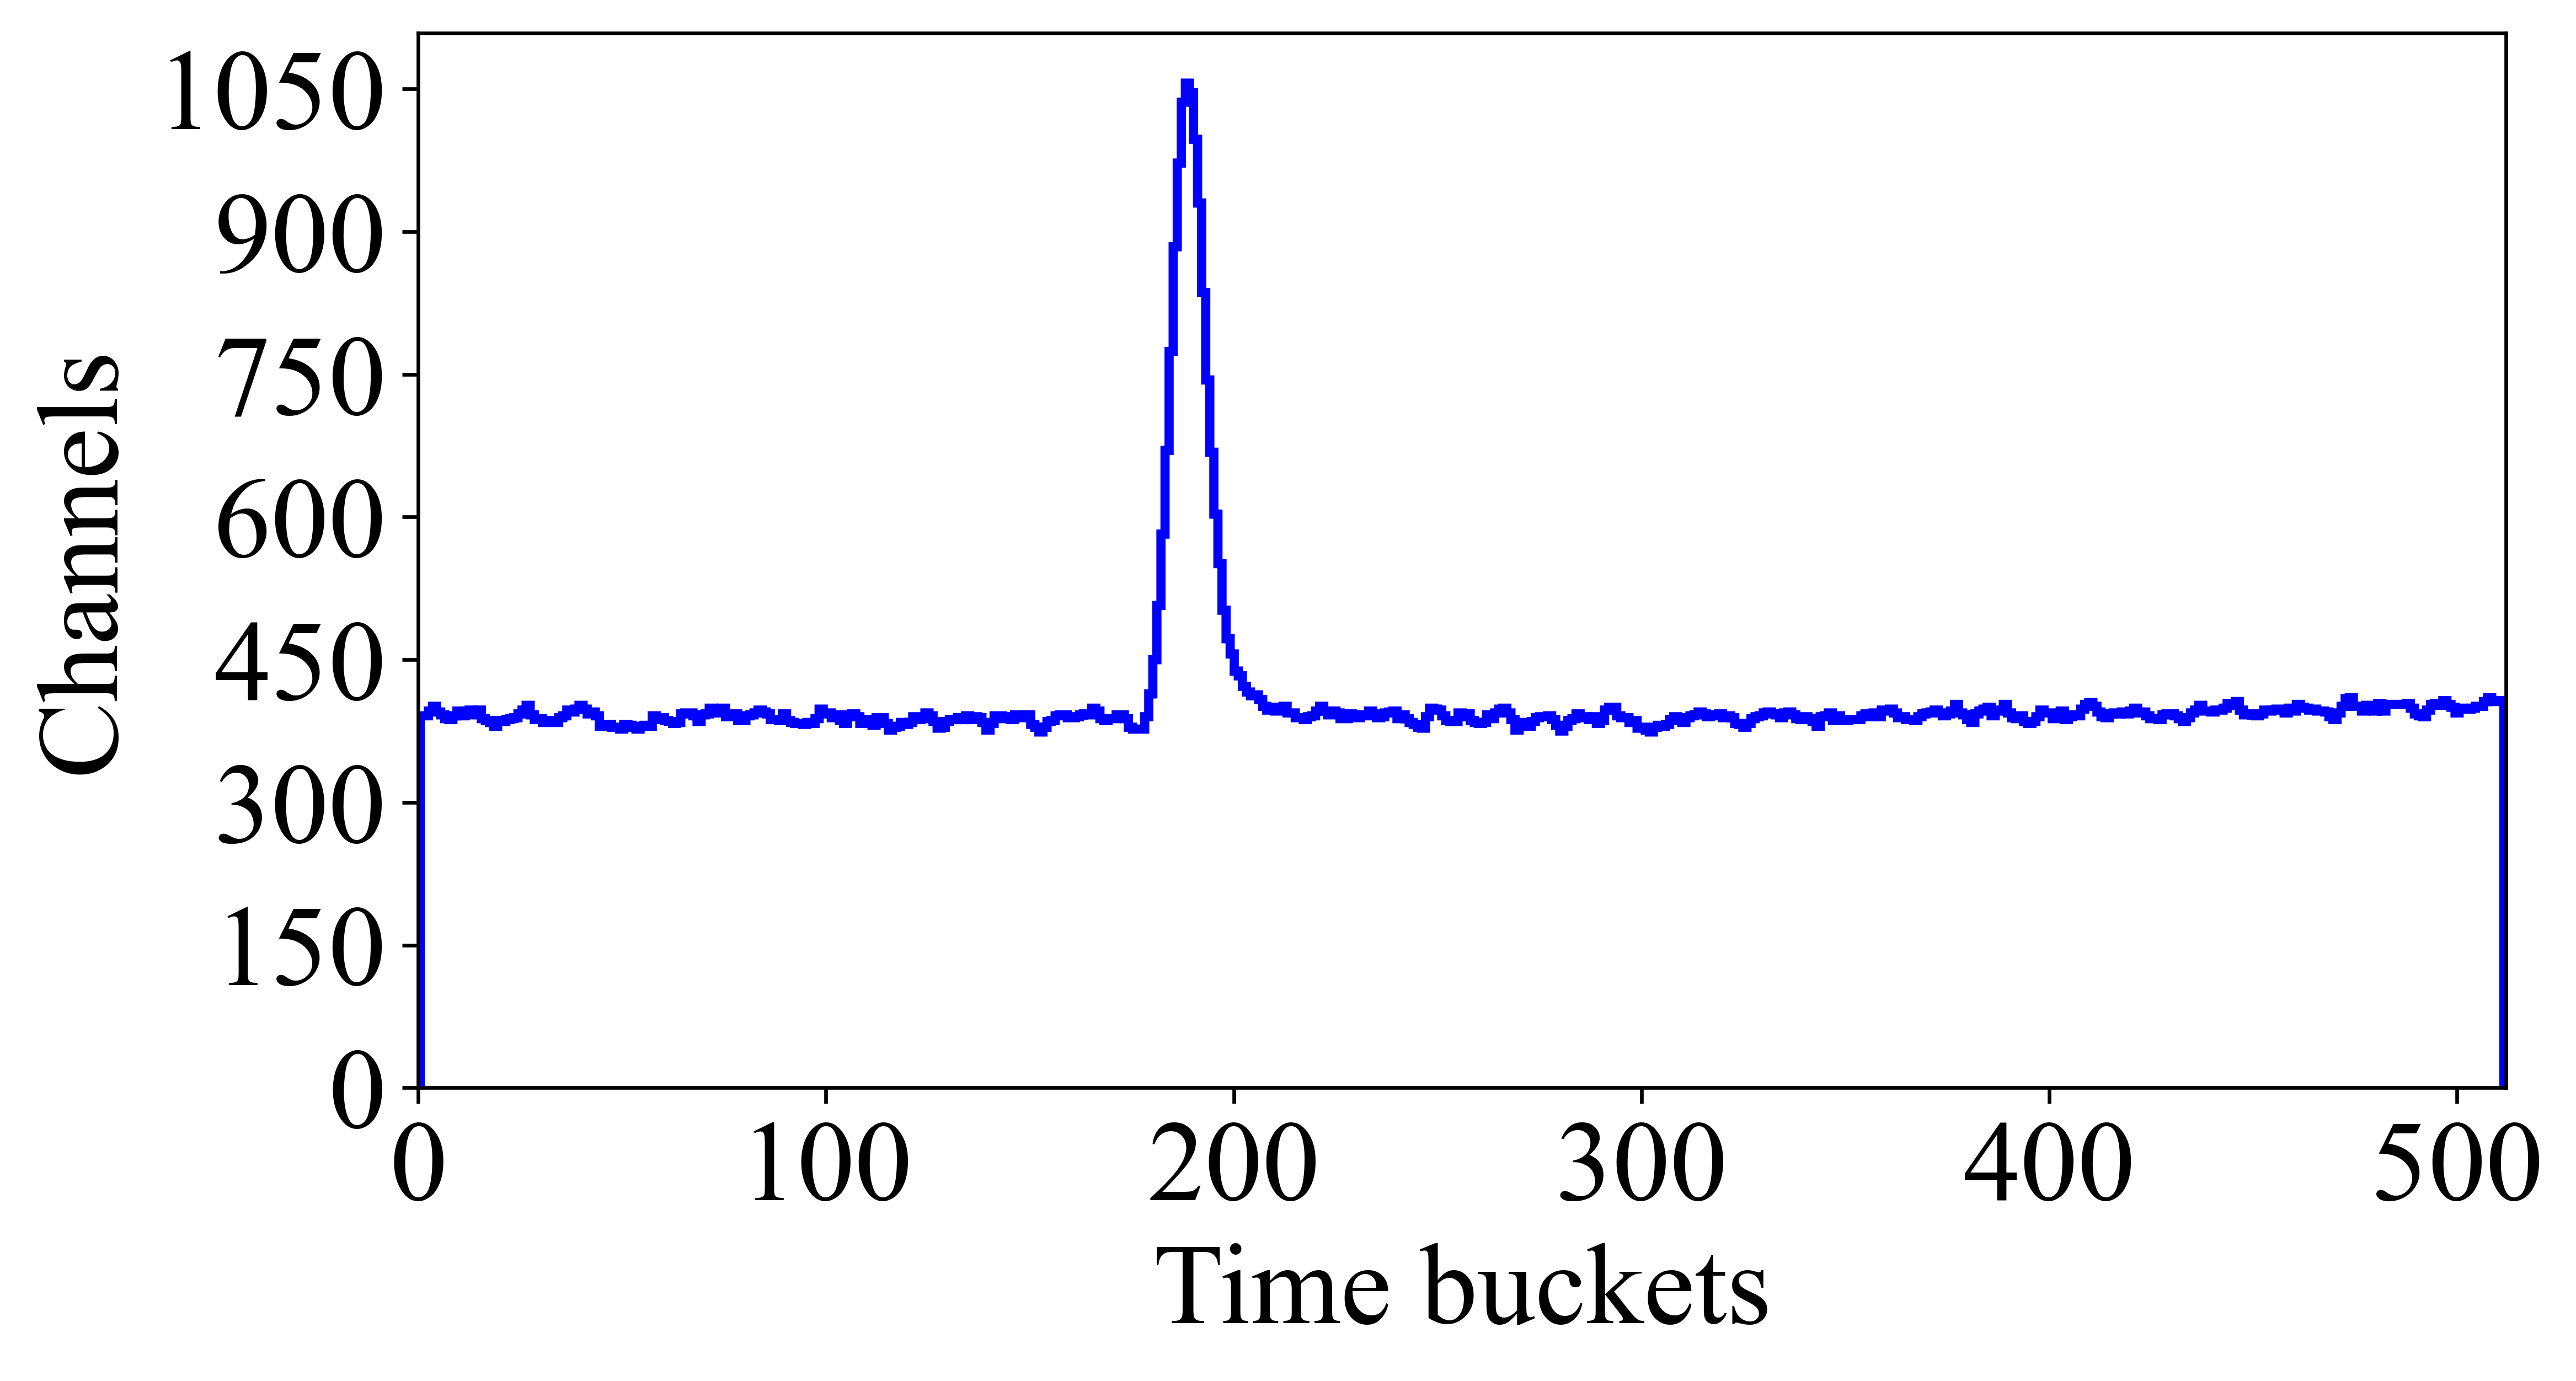
\includegraphics[scale=0.395]{figs/ex_sinal_1.png}
        \caption{}
        \label{subfig:exemplos_sinais_1}
    \end{subfigure}%
    \hfill
    \begin{subfigure}[b]{0.48\textwidth}
        \centering
        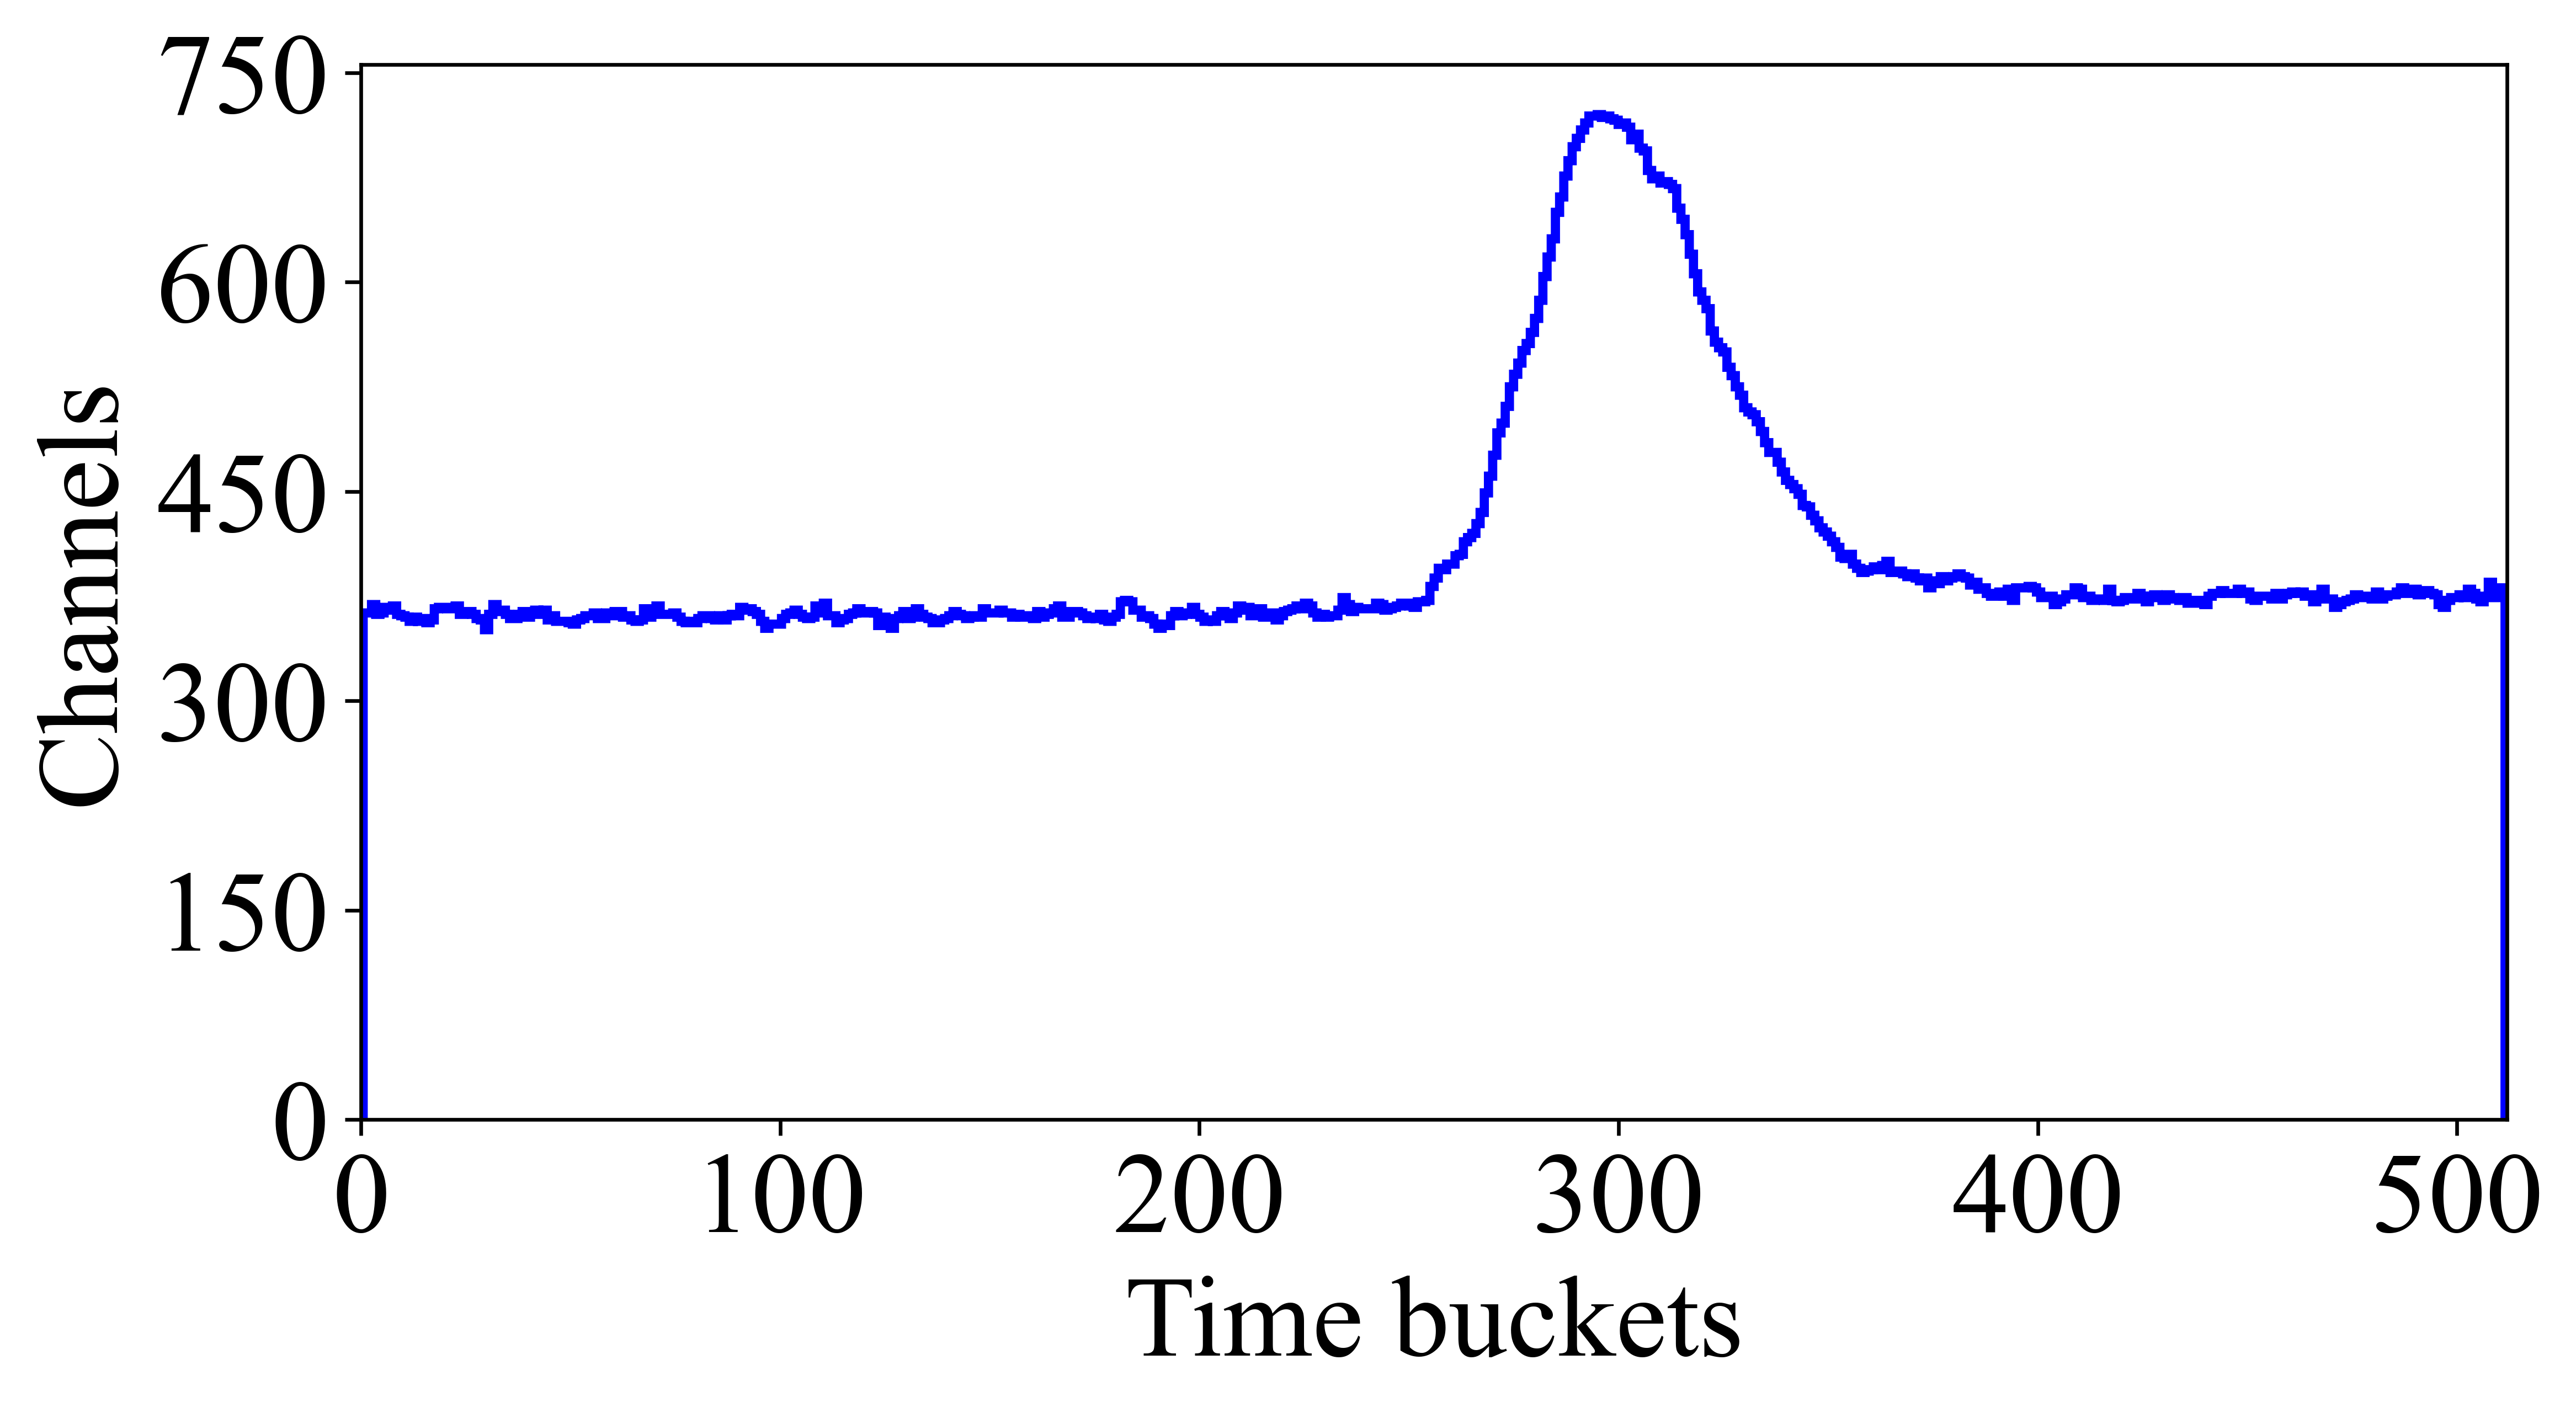
\includegraphics[scale=0.395]{figs/ex_sinal_2.png}
        \caption{}
        \label{subfig:exemplos_sinais_2}
    \end{subfigure}
\caption{Exemplos de sinais produzidos pelos canais do detector. Em \ref{subfig:exemplos_sinais_1} o sinal possui apenas um pulso, enquanto em \ref{subfig:exemplos_sinais_2} há vários pulsos em sobreposição, formando um único pulso com largura maior que em \ref{subfig:exemplos_sinais_1}.}
\label{fig:exemplos_sinais}
\end{figure}

\par No eixo $x$, cada um dos 512 \textit{time buckets} possui largura de 195 $n s$. No eixo $y$ tem-se a carga acumulada no detector para cada \textit{time bucket}. Na figura \ref{subfig:exemplos_sinais_1} há um sinal com um pedestal (fundo ou \textit{baseline}) com altura entre 300 e 450, e um pulso estreito em cima. Como mostrado na seção \ref{PATTPC}, os elétrons que surgiram da ionização do gás foram conduzidos perpendicularmente pelo campo elétrico até o detector. A interação da partícula com o gás é evidenciada justamente pelo pulso presente em \ref{subfig:exemplos_sinais_1}. Cada pixel $i$ do detector está em uma posição ($x_i$, $y_i$), o centroide de cada gaussiana fornece a coordenada em $t$ (\textit{time bucket}) para então ser convertida na posição em coordenada $z$ do ponto de interação da partícula com o gás, e a energia depositada $Q$ é obtida da área do pulso sem fundo (gaussiana com centroide $t$).

\par Para a figura \ref{subfig:exemplos_sinais_1} tem-se apenas um pulso estreito, o que corresponde à um feixe incidindo paralelamente àquele canal do plano detector (perpendicular ao campo elétrico), pois a projeção da interação da partícula com gás no tempo é uma distribuição estreita. No caso da figura \ref{subfig:exemplos_sinais_2}, há uma distribuição ampla do sinal do tempo, o que corresponde ao feixe incidindo perpendicularmente ao canal do plano detector. A ilustração desse processo está na figura \ref{fig:get_signal}, que mostra o processo da passagem de uma partícula carregada e como o sinal é gerado a partir disso.


% único pixel do detector ativado com coordenadas($x$, $y$, $z$). Já para \ref{subfig:exemplos_sinais_2} temos o que é chamado de mistura de gaussianas (\textit{gaussian mixture}), que é a presença de várias gaussianas sobrepostas. Esse tipo de sinal corresponde ao feixe indo perpendicularmente ao pixel do plano do detector, indicando. A ilustração desse processo está na figura \ref{fig:get_signal}, que mostra o processo da passagem de uma partícula carregada e como o sinal é gerado a partir disso.

% As gaussianas presentes em \ref{subfig:exemplos_sinais_2} devem ter a mesma largura da gaussiana presente em \ref{subfig:exemplos_sinais_1}. 

\begin{figure}[H]
    \centering
    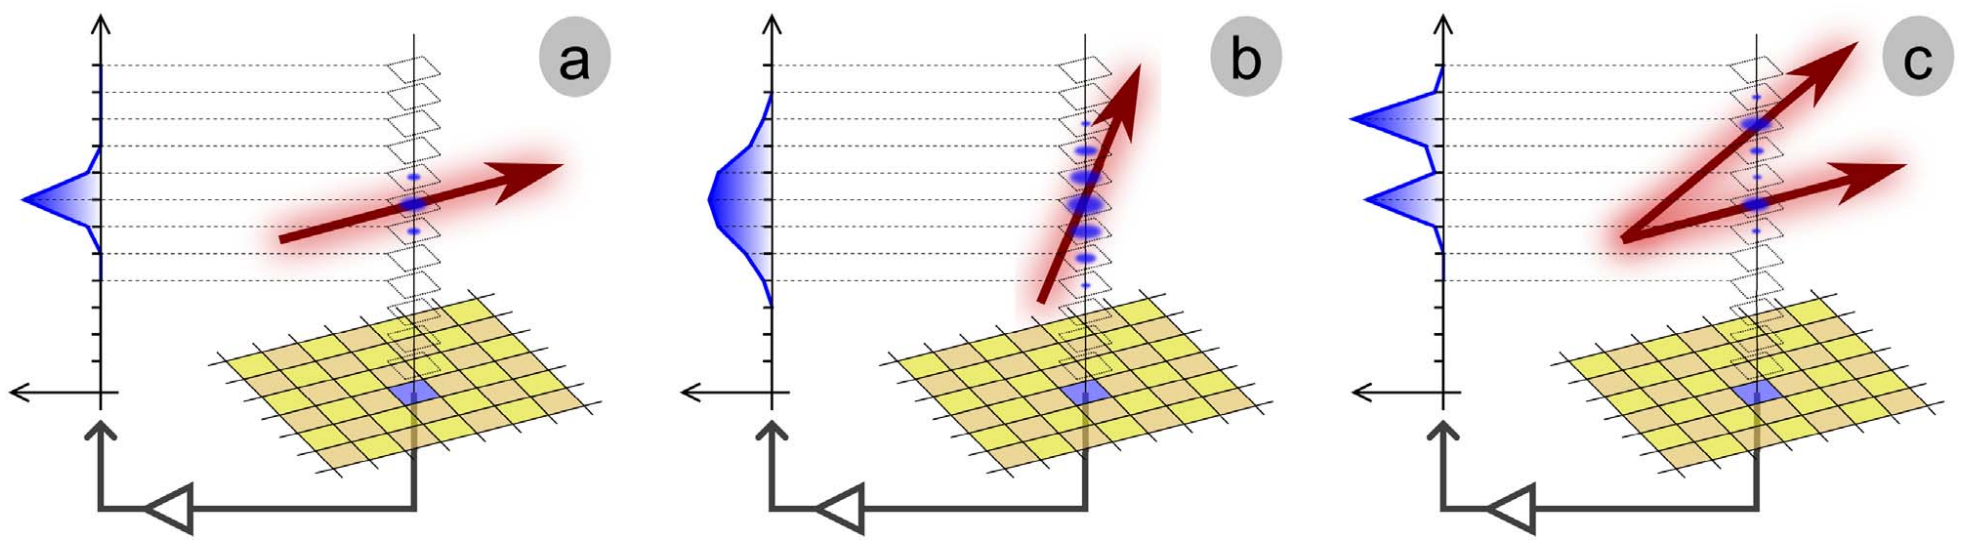
\includegraphics[scale = 0.29]{figs/get.png}
    \caption{Ilustração que mostra a variação no formato da carga coletada a partir da passagem de uma partícula carregada dentro do TPC, onde o plano do detector está embaixo. No lado esquerdo de cada imagem, a distribuição do sinal coletado por um único pad (escuro) do plano de coleta é mostrado (o canal eletrônico de leitura é representado pela seta cinza em negrito). No caso de uma trajetória quase horizontal em relação ao plano do detector (a), o sinal é uma distribuição estreita, enquanto para uma trajetória próxima a uma direção vertical (ou perpendicular) em relação ao detector (b), a distribuição deve ser muito mais ampla (vários pontos de interação da partícula com o gás devem ser extraídos desse sinal). A última imagem ilustra o caso em mais de uma trajetória de partículas contribui para o sinal \cite{GET}.}
    \label{fig:get_signal}
\end{figure}

\par Para analisar os pulsos deve-se primeiro remover o fundo (pedestal ou \textit{baseline}) dos sinais. O sinal de fundo é complexo e pode variar por canal e também por evento. Desde flutuações causadas pelo circuito eletrônico até efeitos sistemáticos gerados pela memória de \textit{buffer} circular alteram o sinal, podendo o tornar não analítico \cite{FORTINO2022166497, GET}. Com o sinal sem o fundo, se faz a deconvolução para determinar todos os centroides e cargas acumuladas dos pontos, para a reconstrução da nuvem de pontos. Todo esse processo foi realizado nesse trabalho com algoritmos de \textit{machine learning} supervisionado\cite{FORTINO2022166497}. Para isso, foi criado um banco de dados que serviu de \textit{output} e/ou \textit{input} para o treino das redes neurais.

\par A criação dos dados para o treino das redes neural está mostrado na seção \ref{subsec:pulses_baseline}. A criação das redes neurais está mostrada na seção \ref{sec:pulsos_ml}. 

% O fundo não é trivial de se determinar, pois não é analítico, oscilando muito entre os canais.

\subsection{Estimativa do fundo}\label{subsec:pulses_baseline}

\par Essa subseção descreve a estimativa do fundo de cada, para formar o banco de dados da rede neural que estima o fundo descrita na subseção \ref{subsec:pulso_ml_fundo}.

\par A primeira tentativa de estimar o sinal sem o fundo é usando transformada de Fourier e um filtro passa-baixa, que é a função resposta do detector fornecida na Ref. \cite{GET}. Seja $f(t)$ uma função qualquer, sua transformada de Fourier é dada por

\begin{equation} \label{eq:fourier}
    \hat{f}(\nu)=\mathscr{F}[f(t)]=\int_{-\infty}^{\infty} f(t) e^{-2 \pi i \nu t} d t.
\end{equation}

\par Primeiro calculamos a transformada de Fourier $\hat{f}(\nu)$ do sinal, em seguida multiplicamos pela função resposta do detector $h(\nu)$ dada por \cite{GET}

\begin{equation}
    h(\nu) = A*\exp\left (\nu \tau \right)\left(\nu \tau\right)^3 \sin \left( \nu \tau \right) ,
\end{equation}

%\begin{equation}
%    \sinc x \equiv \frac{\sin (\pi x)}{\pi x},
%\end{equation}

\par onde $A$ está relacionado com o ganho de amplificação e $\tau$ é o tempo de pico (\textit{peaking time}), que é o tempo de modelagem da cadeia de amplificação \cite{GET}. Do teorema da convolução, temos que \cite{metodos_mat_aplicada}

%\par onde $a$ é um fator de escala. A função sinc foi escolhida para tirar vantagem do Teorema da Convolução, dado por\cite{metodos_mat_aplicada}

\begin{equation}
    \mathscr{F}^{-1}[\hat{f}(\nu) \hat{g}(\nu)]=(f * g)(t)=\int_{-\infty}^{\infty} f(\tau) g(t-\tau) d \tau, 
\end{equation}

\par onde $(f * g)(t)$ é a convolução entre $f(t)$ e $g(t)$. Multiplicar o sinal transformado por $h(\nu)$ e depois inverter inverter a transformação é o mesmo que convoluir o sinal original com a transformação inversa de $h(\nu)$, o que resulta no sinal sem o fundo \cite{josh_bradt, GET}. Resultados desse procedimento estão na figura \ref{fig:bs_fourier_exs}.

%Multiplicar o sinal transformado por $\sinc (\nu / a)$ e depois inverter inverter a transformação é o mesmo que convoluir o sinal original com a transformação inversa de $\sinc (\nu / a)$, pois

%\begin{equation}
%\mathscr{F}^{-1}[\sinc(\nu)]=\rect(t) \equiv \begin{cases}1, & -\frac{1}{2}<t<\frac{1}{2} \\ 0, & \text { qualquer outro }t\end{cases},
%\end{equation}
%
%é uma função que representa uma janela retangular, o que seria um exemplo de função resposta do detector. Caso saibamos essa função resposta, então é possível reconstruir completamente o sinal. Resultados desse procedimento estão na figura \ref{fig:bs_fourier_exs}.

\begin{figure}[H]
\centering
    \begin{subfigure}[c]{0.45\textwidth}
        % \centering
        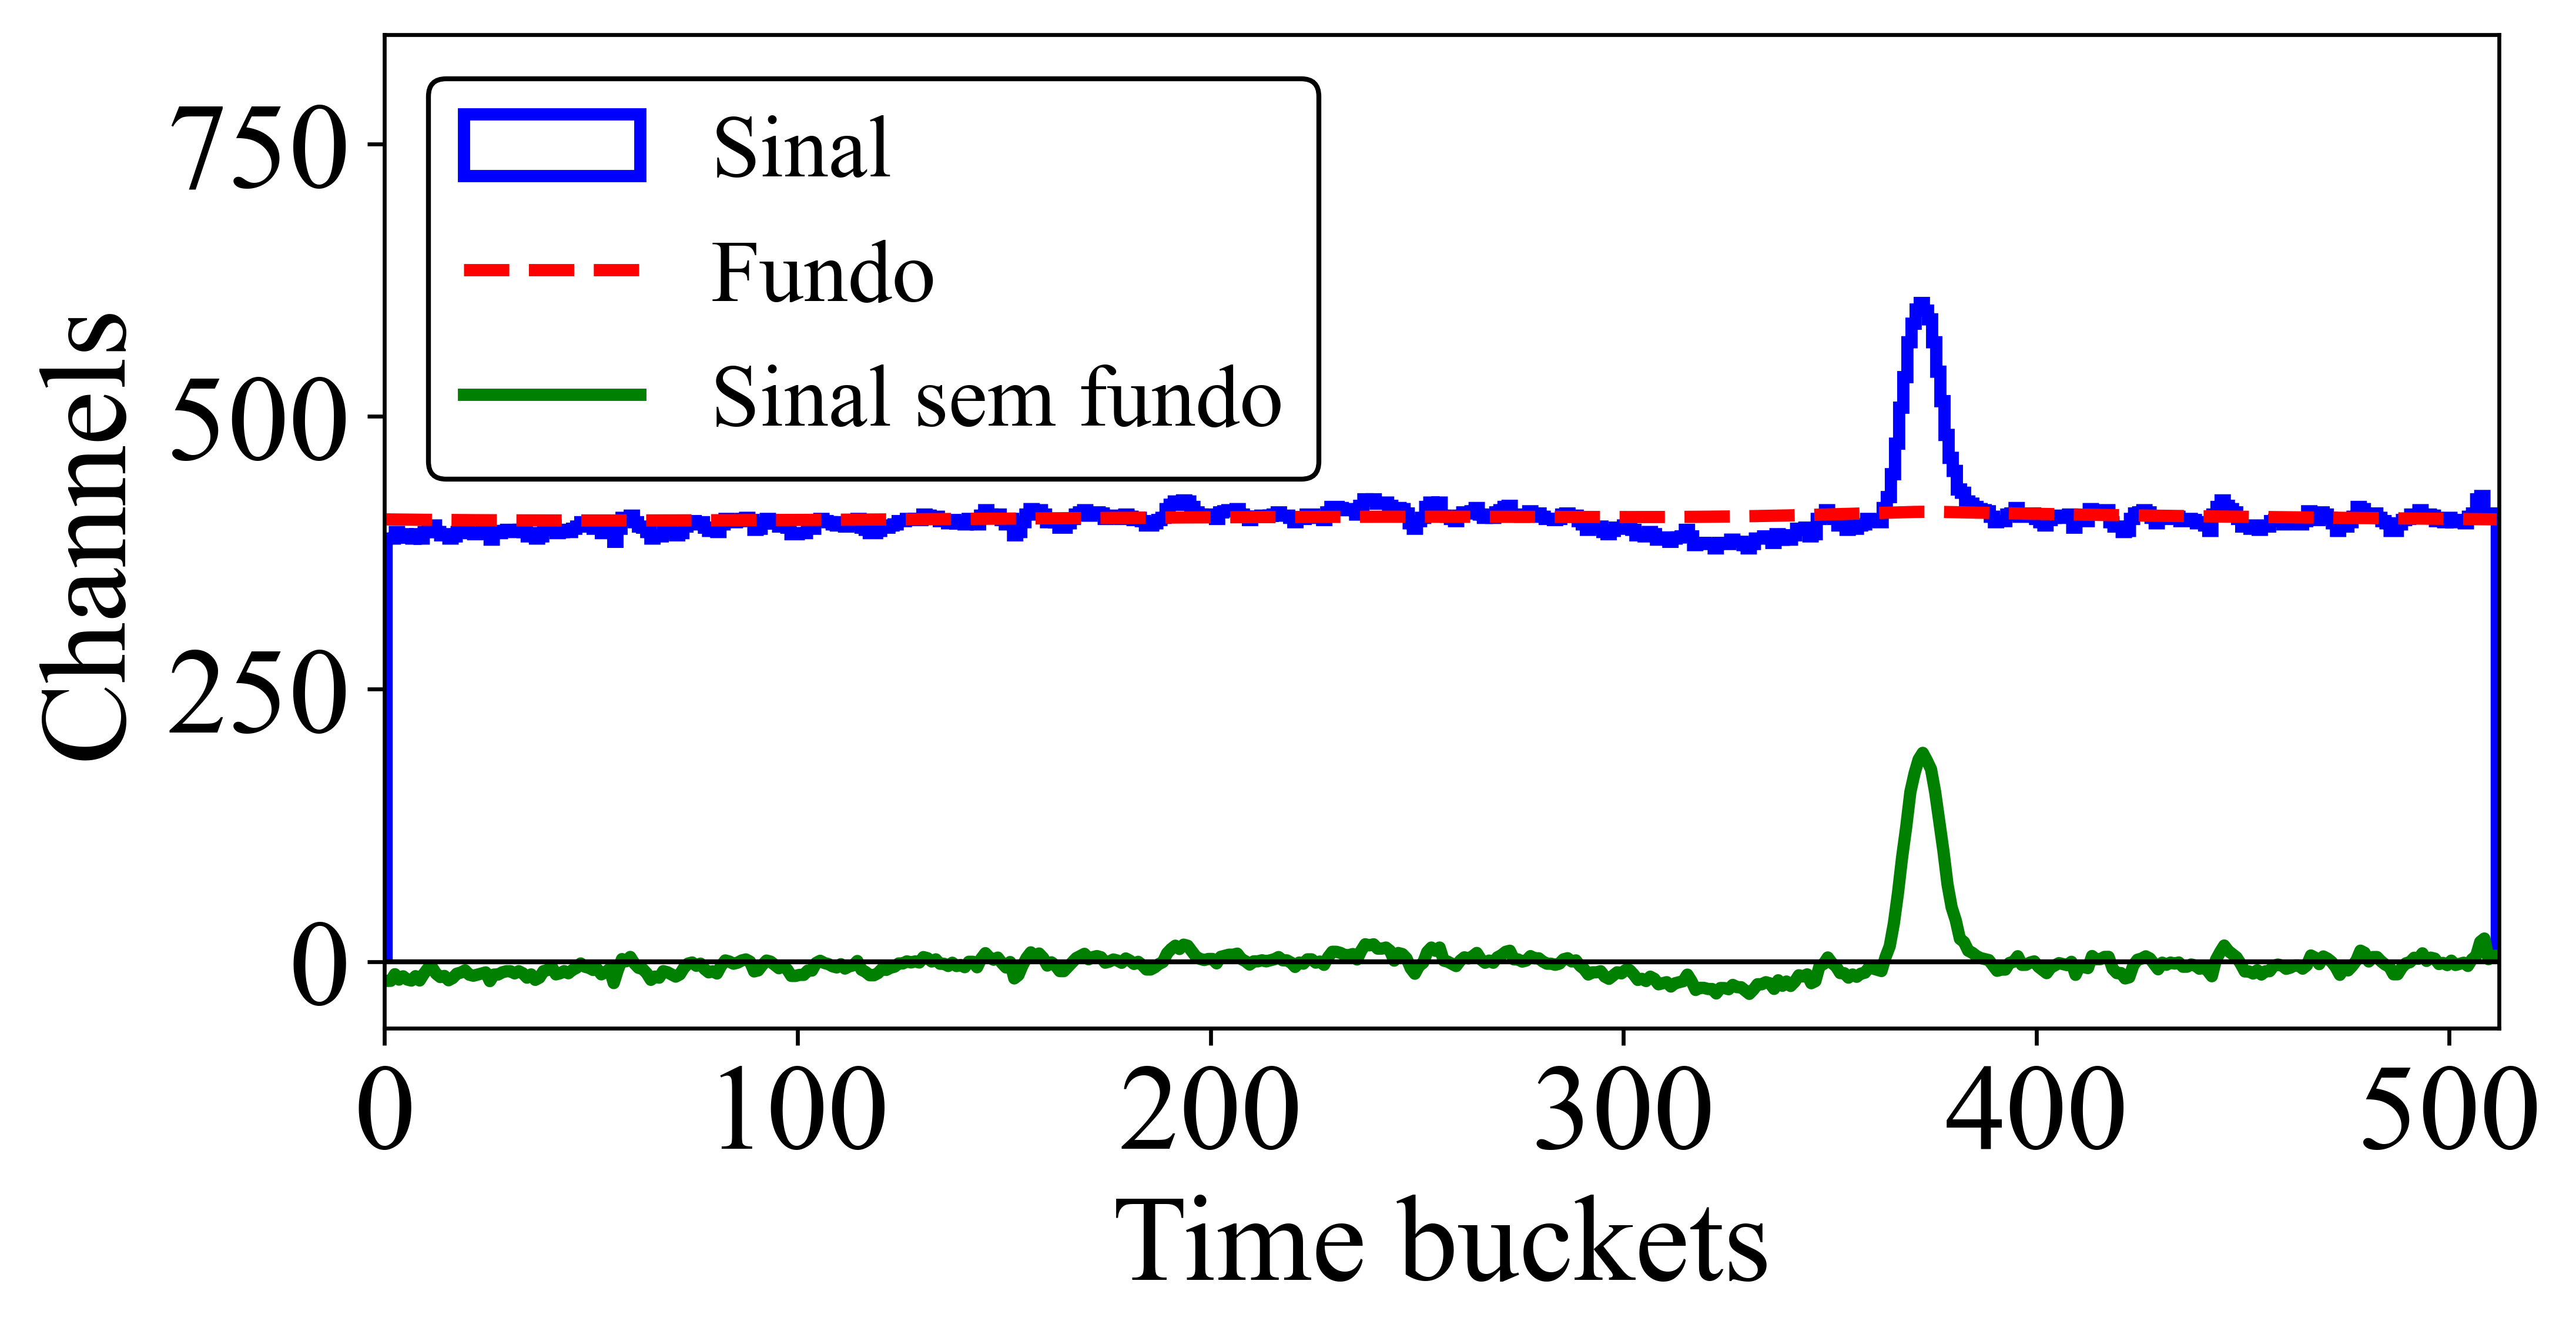
\includegraphics[scale=0.42]{figs/bs_fourier_1.png}
        \caption{}
        \label{subfig:bs_fourier_1}
    \end{subfigure}%
    \hfill
    \begin{subfigure}[c]{0.45\textwidth}
        % \centering
        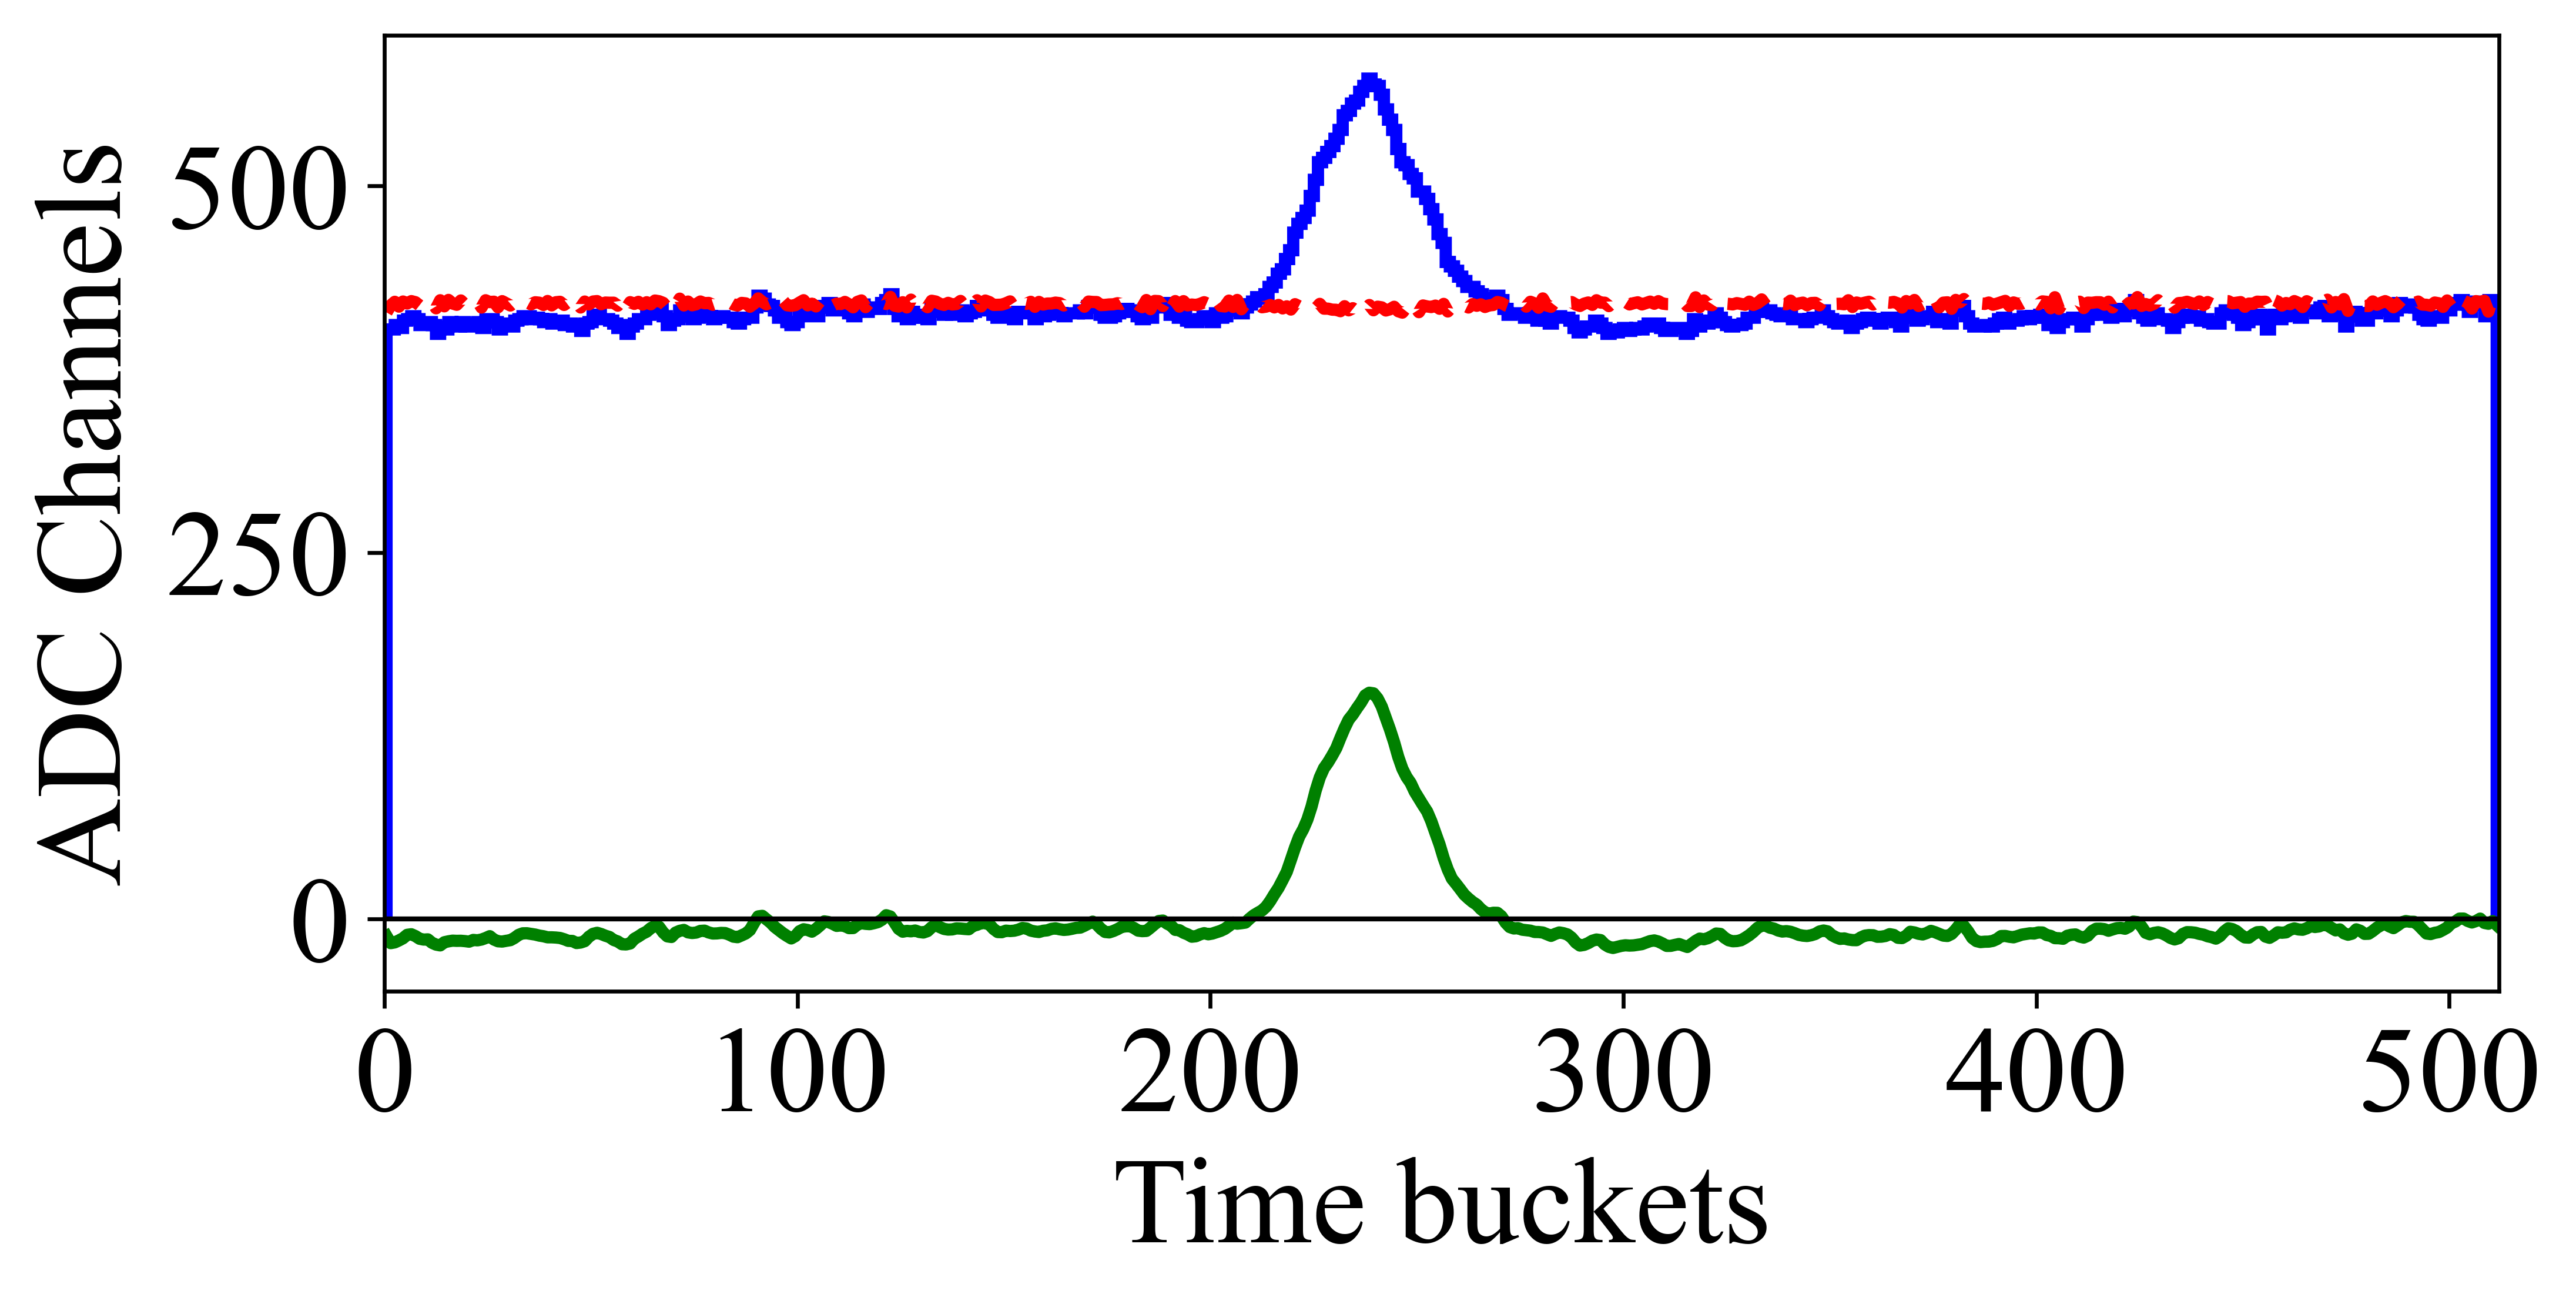
\includegraphics[scale=0.42]{figs/bs_fourier_2.png}
        \caption{}
        \label{subfig:bs_fourier_2}
    \end{subfigure}
    \begin{subfigure}[b]{0.45\textwidth}
        \centering
        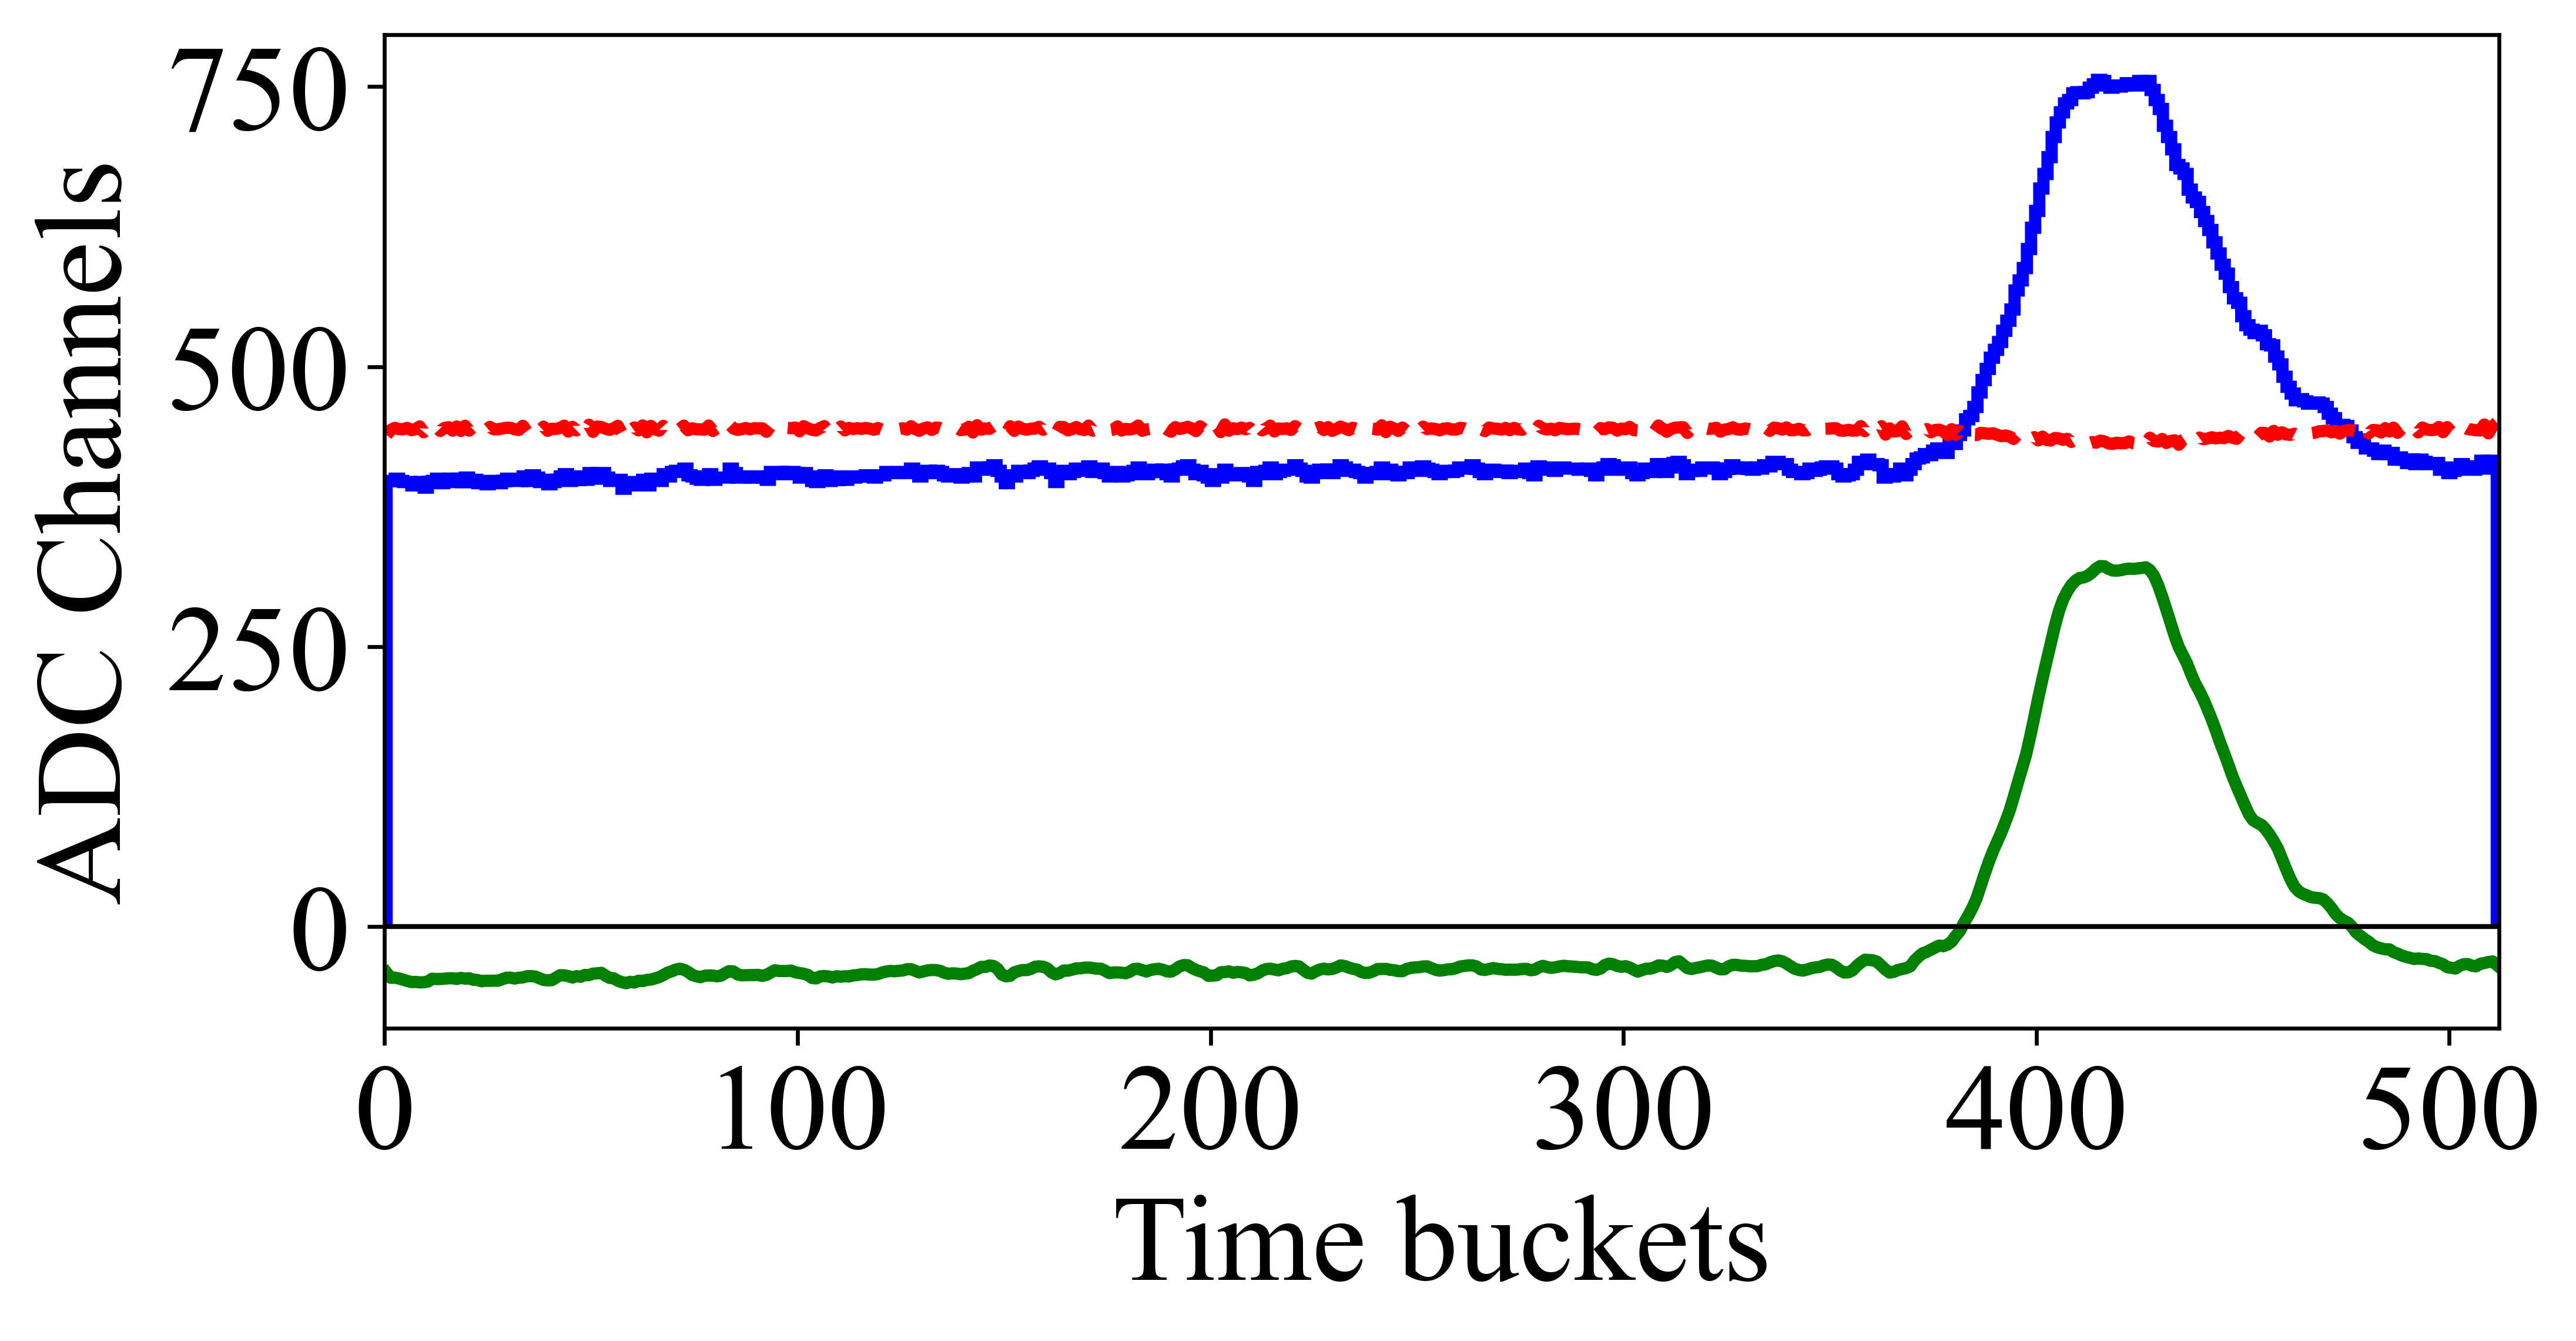
\includegraphics[scale=0.42]{figs/bs_fourier_3.png}
        \caption{}
        \label{subfig:bs_fourier_3}
    \end{subfigure}%
    \hfill
    \begin{subfigure}[b]{0.45\textwidth}
        \centering
        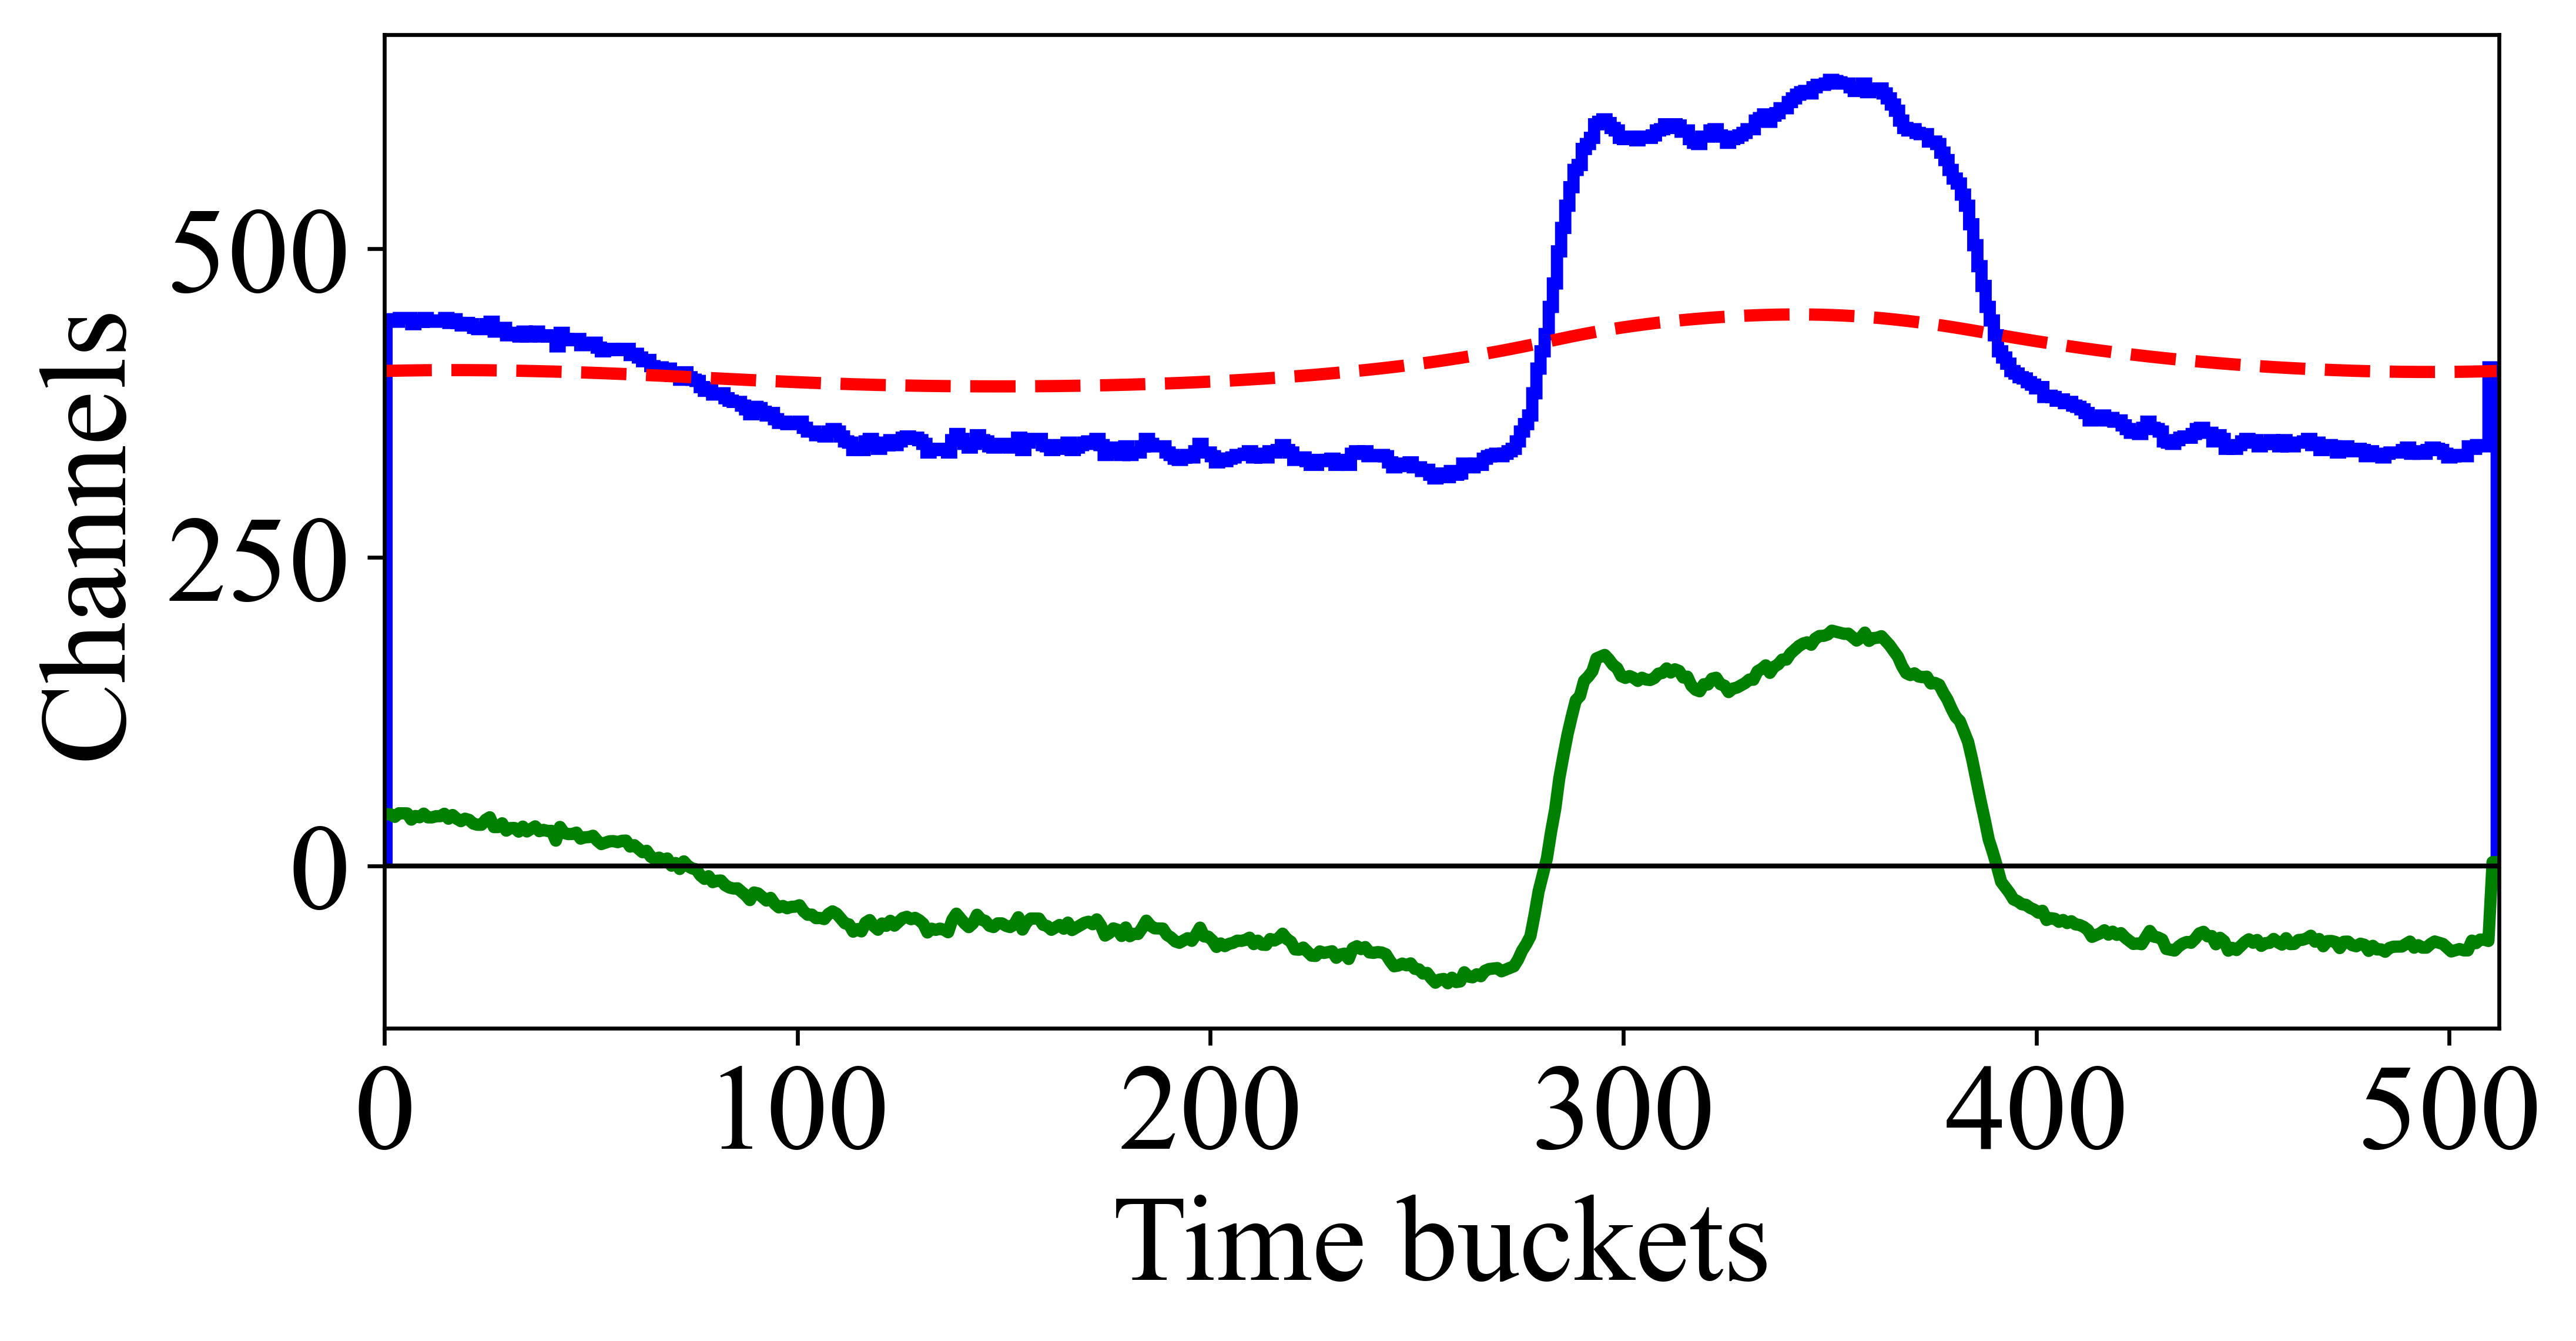
\includegraphics[scale=0.42]{figs/bs_fourier_4.png}
        \caption{}
        \label{subfig:bs_fourier_4}
    \end{subfigure}
\caption{Histogramas com as respectivas \textit{baselines} (linhas tracejadas) estimadas pelo método da convolução. O espectro resultante (sem o fundo) está em verde.}
\label{fig:bs_fourier_exs}
\end{figure}

% Dos exemplo acima em muitos casos, acaba estimando o sinal original, na região do pulso, menor do que deveria ser, fazendo com que o sinal tenha menos carga do que deveria.

\par Fica claro que visualmente, por exemplo na figura \ref{subfig:bs_fourier_4}, que o filtro utilizado não é a melhor função resposta do detector. Poderia-se estimar essa função resposta empiricamente, porém os canais auxiliares chamados de \textit{Fixed Pattern Noise} (FPN) \cite{GET} usados para esta estimativa não foram armazenados. Portanto, a estimativa do fundo foi feita sinal por sinal\cite{FORTINO2022166497, GET}. Para isso, o fundo foi determinado usando o algoritmo \textit{background removal} da biblioteca \textit{TSpectrum} do \textit{ROOT} \cite{root}. A função tem a capacidade de separar o fundo dos picos presentes no espectro \cite{BKG_1, BKG_2, BKG_3}. Exemplos de estimativa do fundo estão na figura \ref{fig:ex_sinal_bkg}.

%, pois o fundo é não analítico\cite{GET}. Para um resultado mais adequado, o fundo será determinado usando o algoritmo \textit{background removal} da biblioteca \textit{TSpectrum} do \textit{ROOT} \cite{root}. A função tem a capacidade de separar o fundo dos picos presentes no espectro\cite{BKG_1, BKG_2, BKG_3}. Exemplos de estimativa do fundo estão na figura \ref{fig:ex_sinal_bkg}.

\begin{figure}[H]
\centering
    \begin{subfigure}[b]{0.48\textwidth}
        \centering
        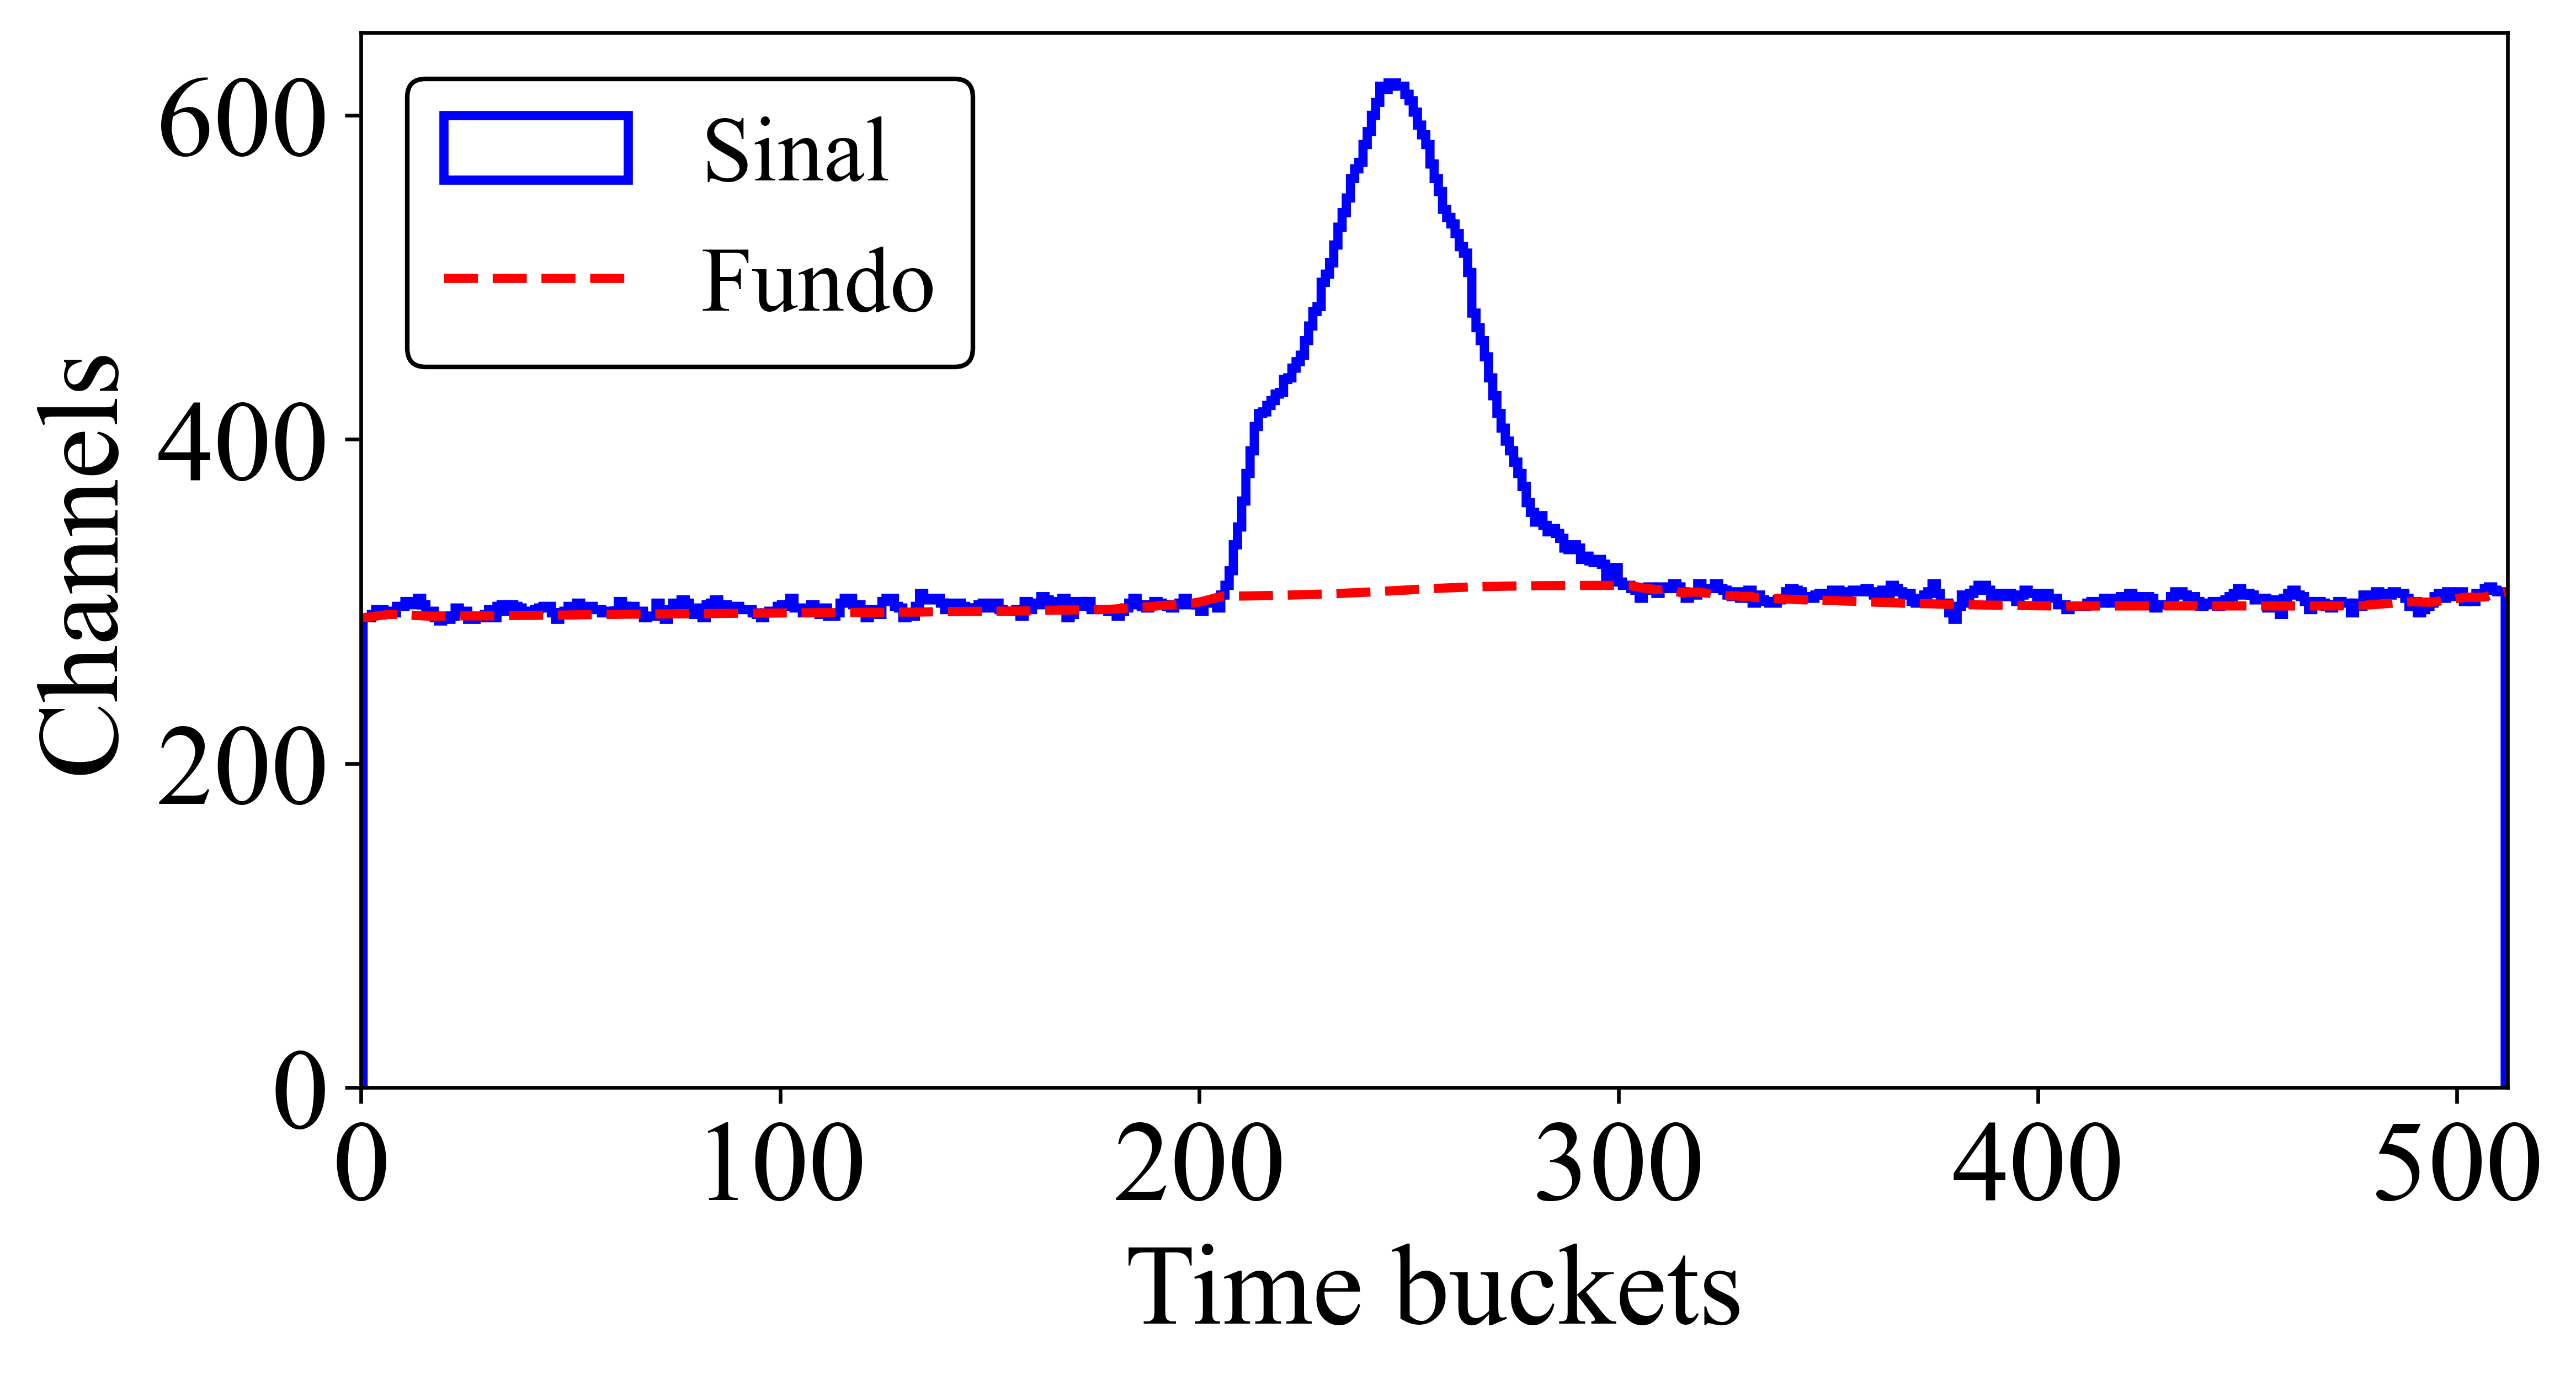
\includegraphics[scale=0.394]{figs/ex_sinal_bkg_1.png}
        \caption{}
        \label{subfig:ex_sinal_bkg_1}
    \end{subfigure}%
    \hfill
    \begin{subfigure}[b]{0.48\textwidth}
        \centering
        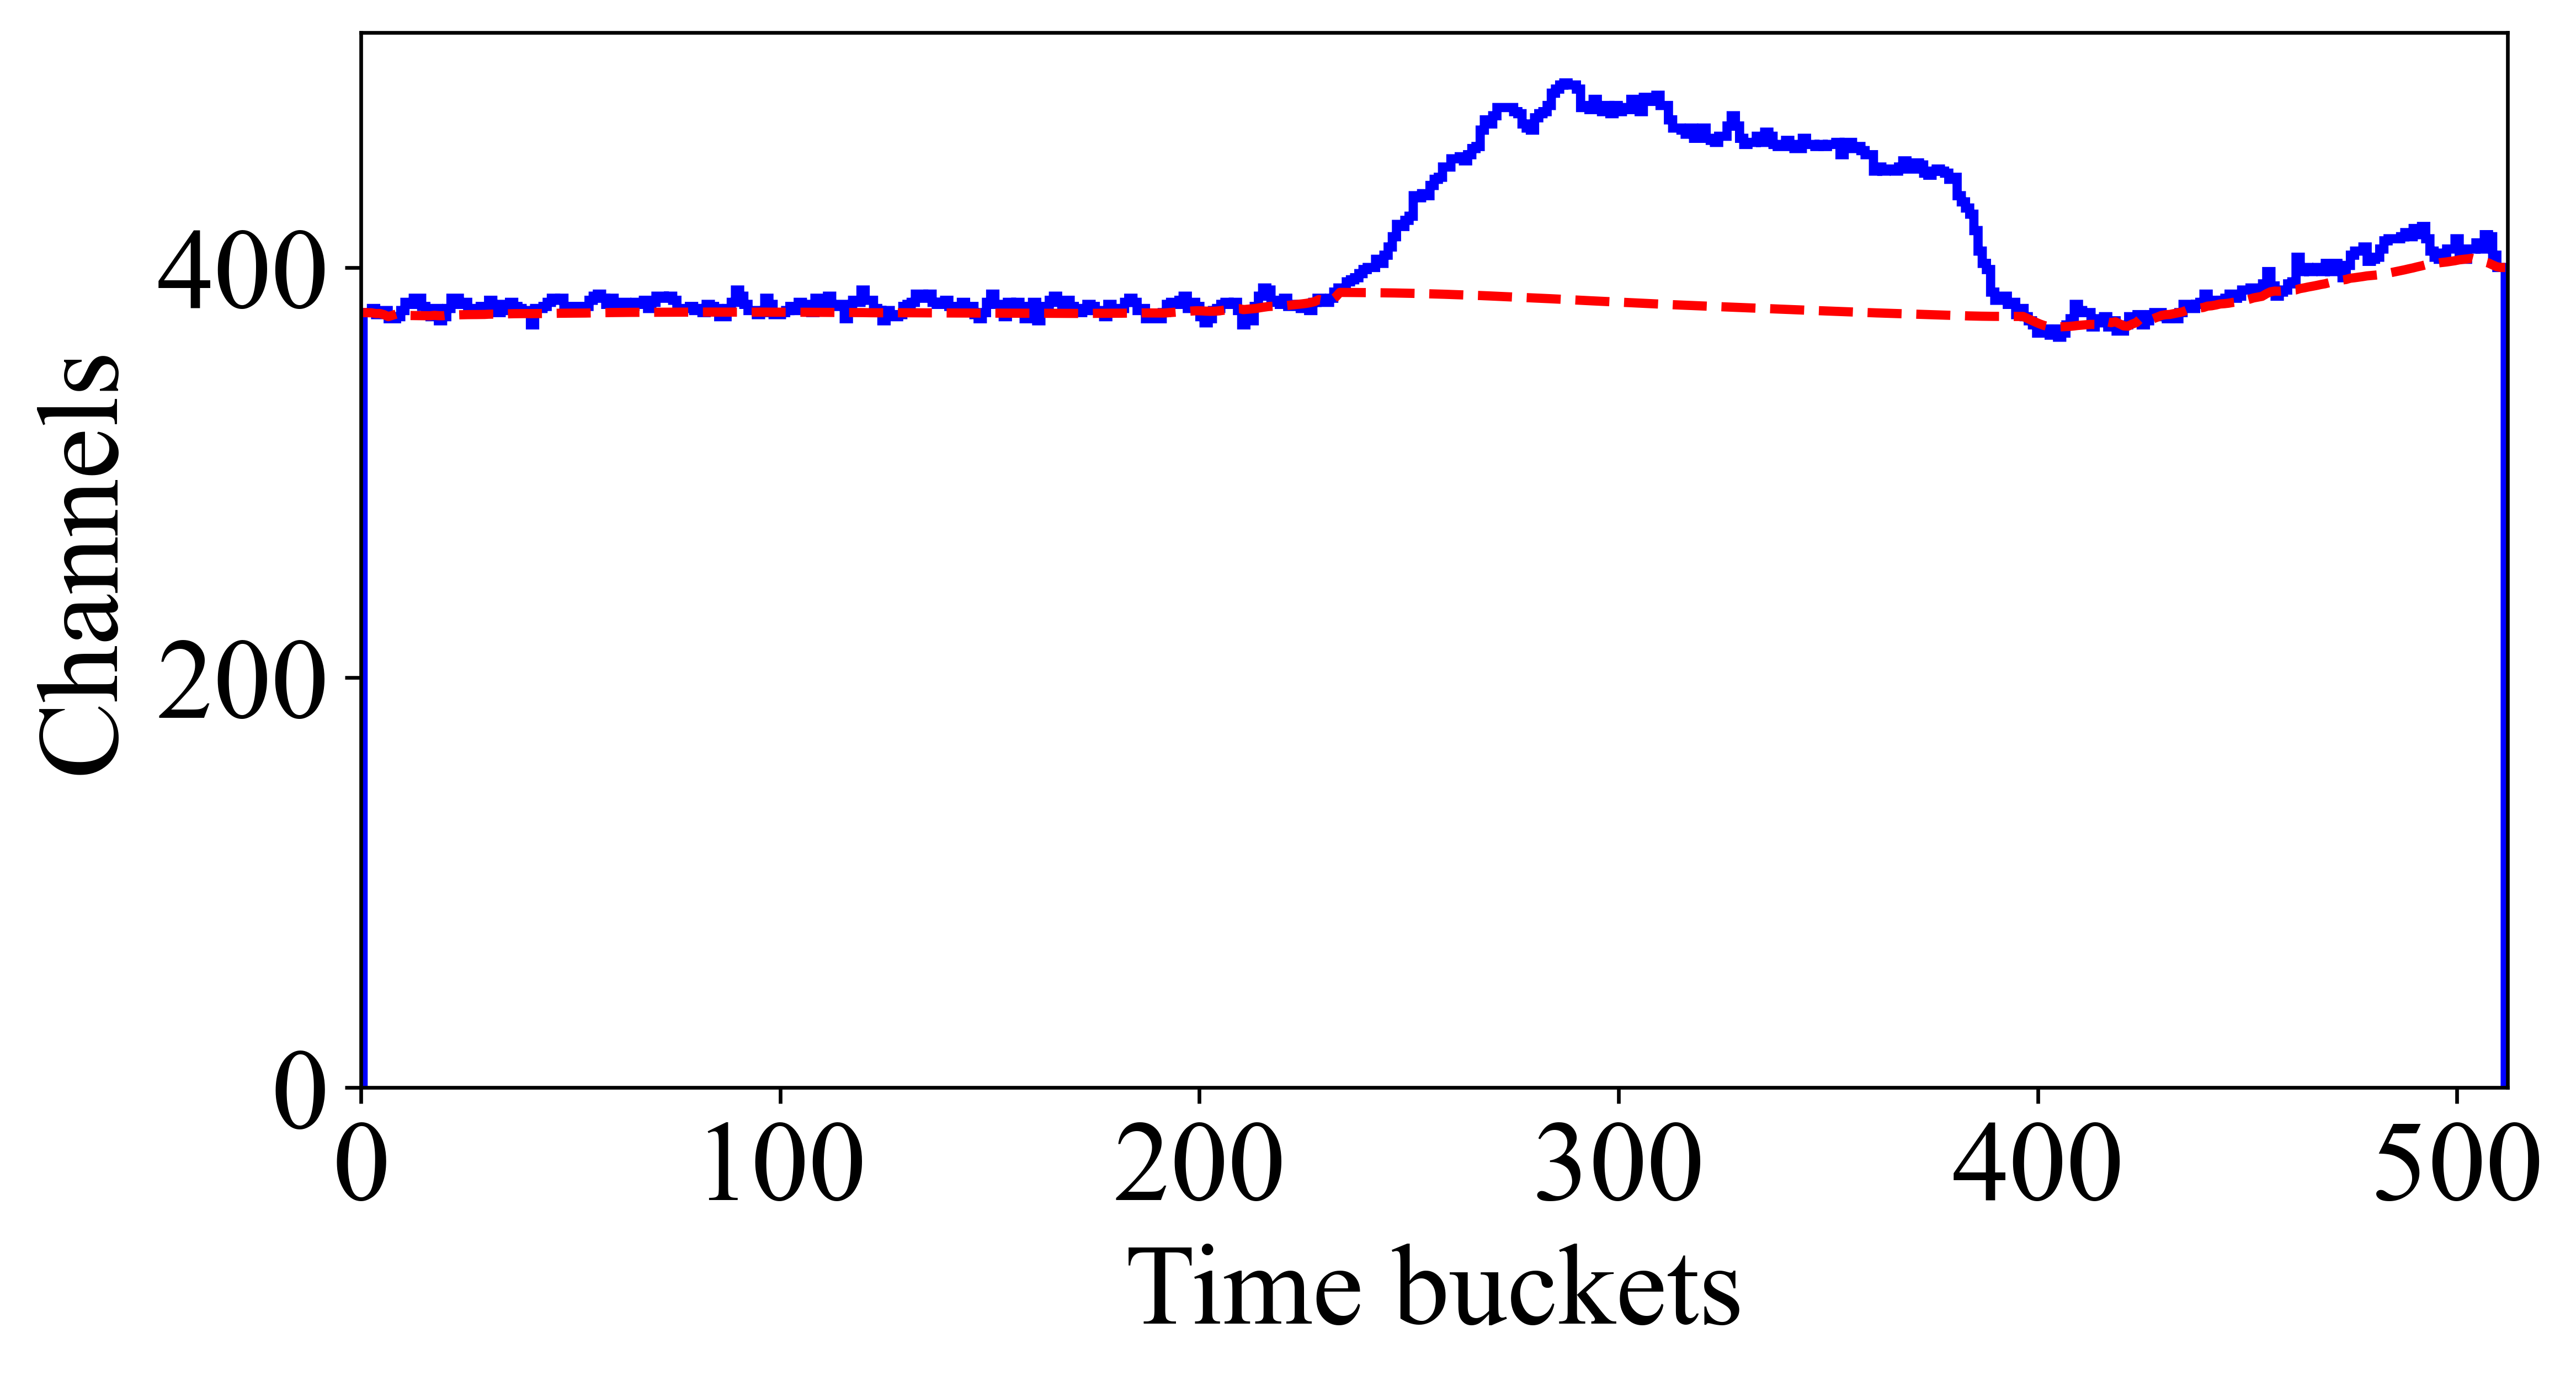
\includegraphics[scale=0.394]{figs/ex_sinal_bkg_2.png}
        \caption{}
        \label{subfig:ex_sinal_bkg_2}
    \end{subfigure}
    \begin{subfigure}[b]{0.48\textwidth}
        \centering
        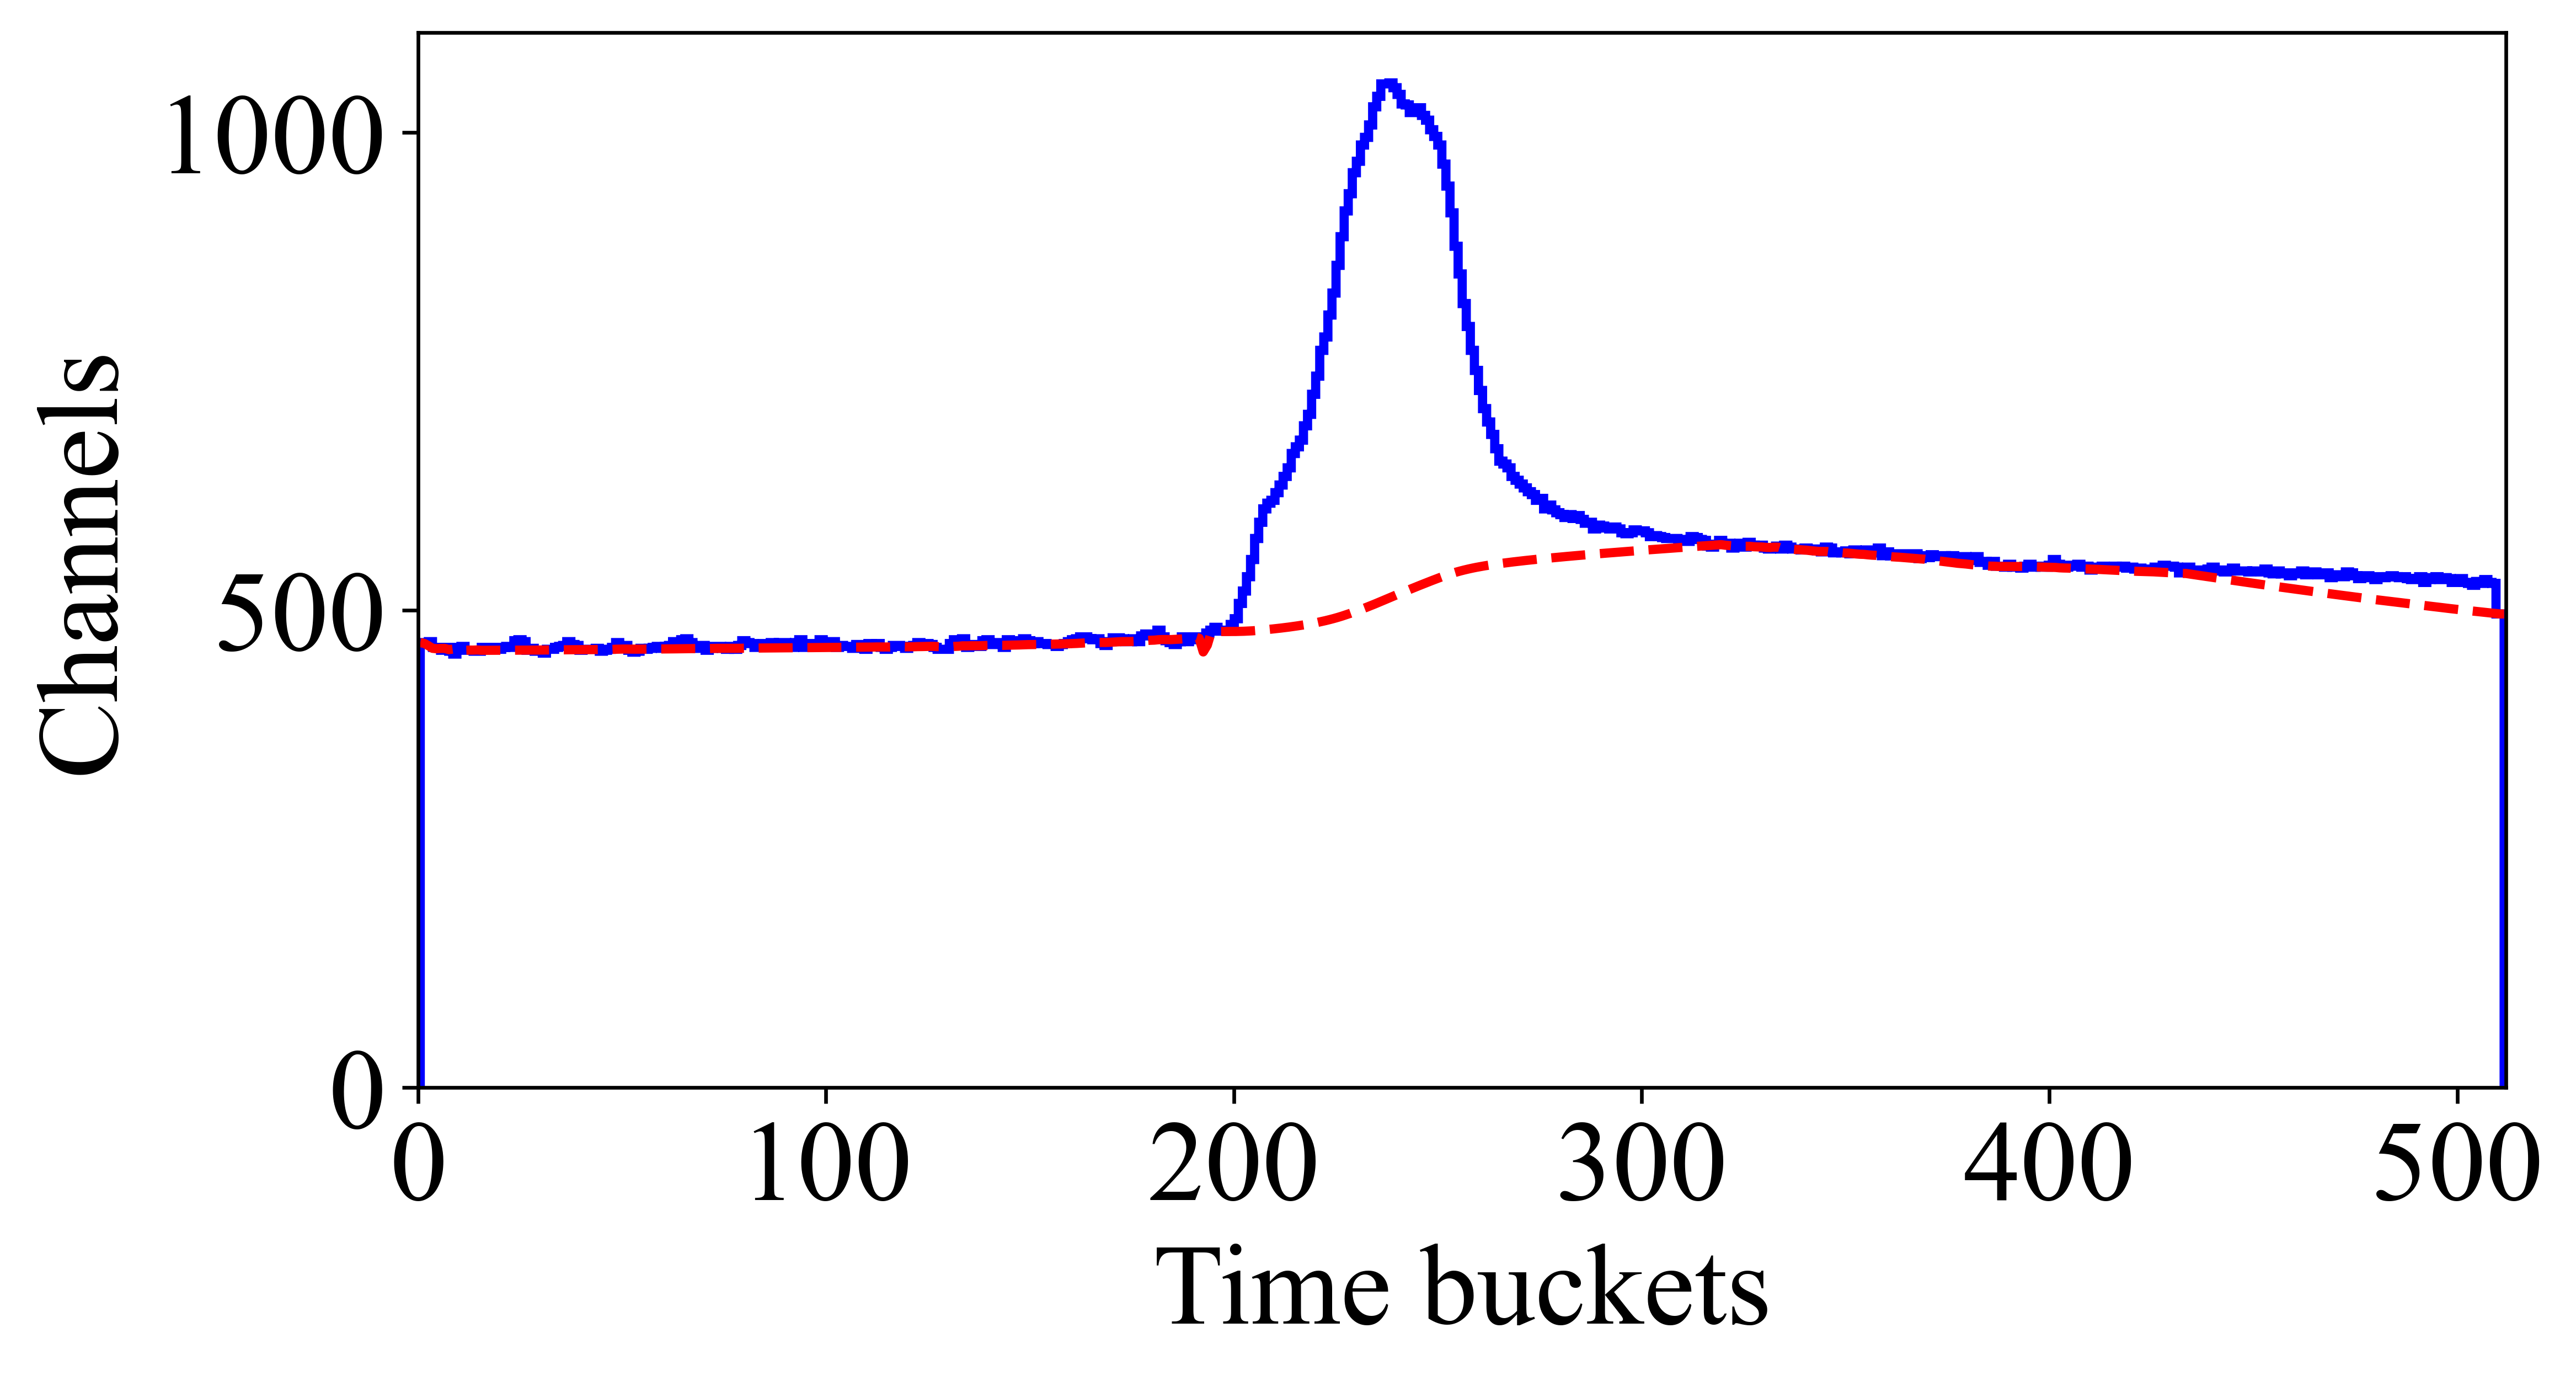
\includegraphics[scale=0.394]{figs/ex_sinal_bkg_3.png}
        \caption{}
        \label{subfig:ex_sinal_bkg_3}
    \end{subfigure}%
    \hfill
    \begin{subfigure}[b]{0.48\textwidth}
        \centering
        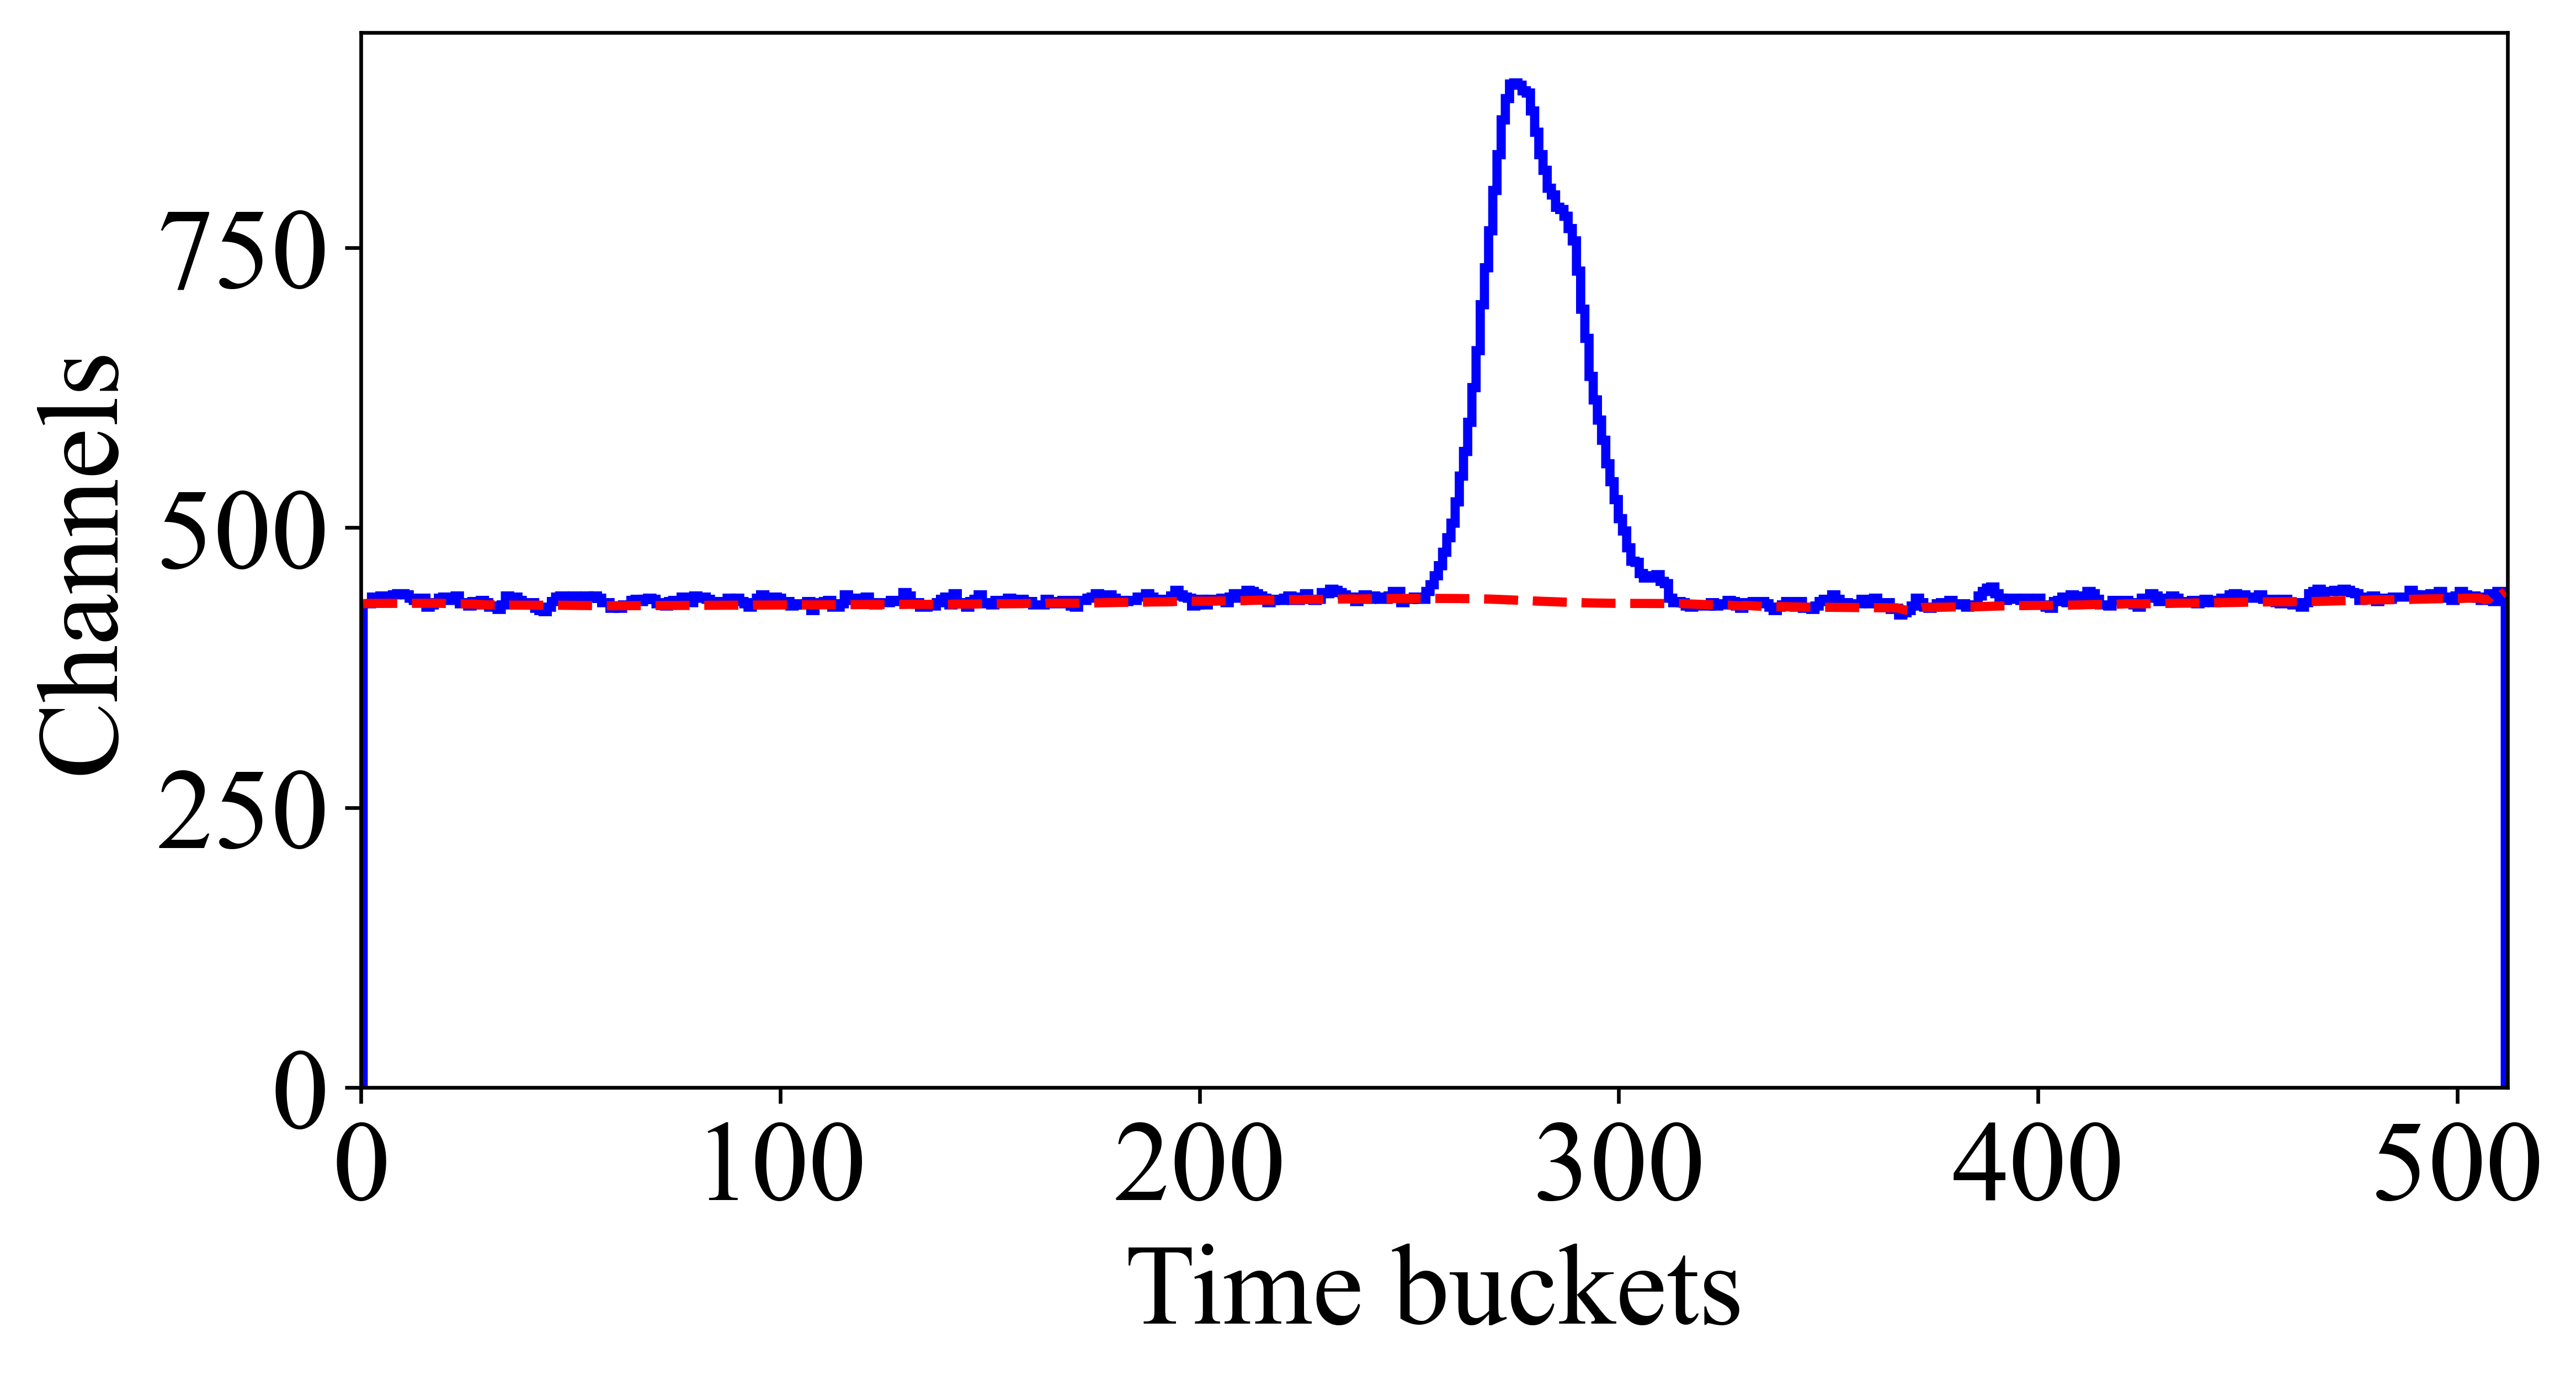
\includegraphics[scale=0.394]{figs/ex_sinal_bkg_4.png}
        \caption{}
        \label{subfig:ex_sinal_bkg_4}
    \end{subfigure}
\caption{Histogramas com as respectivas \textit{baselines} (linhas tracejadas) calculadas pelo \textit{TSpectrum}.}
\label{fig:ex_sinal_bkg}
\end{figure}

\par Os resultados do calculo do fundo de cada sinal foram armazenados e usados para a etapa de deconvolução do sinal, que deve ser feita com o sinal sem o fundo. Para diminuir as flutuações numéricas após a remoção do fundo, o valor mínimo do sinal sem o fundo é zero. Sem o fundo podemos buscar por todos os picos e suas cargas correspondentes no sinal. Não podemos identificar diretamente todos os picos pois muitos deles estão em sobreposição. Para isso foi feita a deconvolução do sinal, descrita na subseção \ref{subsec:pulses_deconv}.

% \par Com o fundo podemos então subtraí-lo do espectro. Podem aparecer valores negativos após a retirada do fundo, então para evitar esse problema o valor mínimo do sinal, após a retirada do fundo, é zero.


\subsection{Deconvolução do sinal}\label{subsec:pulses_deconv}

%\par Essa subseção descreve a etapa de deconvolução do sinal, que serve de banco de dados para o treinamento da rede neural descrita na subseção \ref{subsec:pulso_ml_deconv}.

\par Para aumentar a resolução dos picos foi usado o algoritmo \textit{gold deconvolution} presente na biblioteca \textit{TSpectrum} do \textit{ROOT} \cite{paper_gold_deconv}. O algoritmo tem como objetivo fazer a deconvolução do espectro, gerando uma função (nesse caso um sinal) resposta de acordo com o sigma esperado para os pulsos. O sinal resposta corresponde ao espectro com as gaussianas não sobrespostas. Isso significa que foi necessário determinar qual o valor de sigma dos pulsos para buscar a função resposta.

\par A largura dos pulsos é o mesmo de um sinal que possui apenas um pico. Ou seja, a largura dos pulsos foi determinada fazendo a análise de sinais que possuem apenas 1 pico, fazendo um ajuste pelo método dos mínimos quadrados (MMQ) de uma gaussiana. Para buscar espectros com apenas um pico, foi usado o algoritmo de identificação de picos \textit{peak\_finder}, presente na biblioteca do \textit{scipy} \cite{scipy}, e para o ajuste da gaussiana foi usada o pacote \textit{lmfit} \cite{lmfit}. O valor de sigma encontrado foi de 4.09 (17) \textit{time buckets}.

\par A largura escolhida foi ligeiramente maior pois, verificando empiricamente, em alguns casos o algoritmo separava o que deveria ser uma única gaussiana em duas. O valor de sigma usado na deconvolução foi de 4.30 \textit{time buckets}. Foi determinado também o número de iterações do algoritmo de deconvolução. O número de iterações escolhido foi de 700, menos que isso o algoritmo não estava separando totalmente picos sobrepostos. O limiar para a escolha de um ponto como um pico foi definido como ter altura maior que 20\% do valor máximo do sinal. Resultados da deconvolução estão na figura \ref{fig:ex_sinal_deconv}.

\begin{figure}[H]
\centering
    \begin{subfigure}[b]{0.48\textwidth}
        \centering
        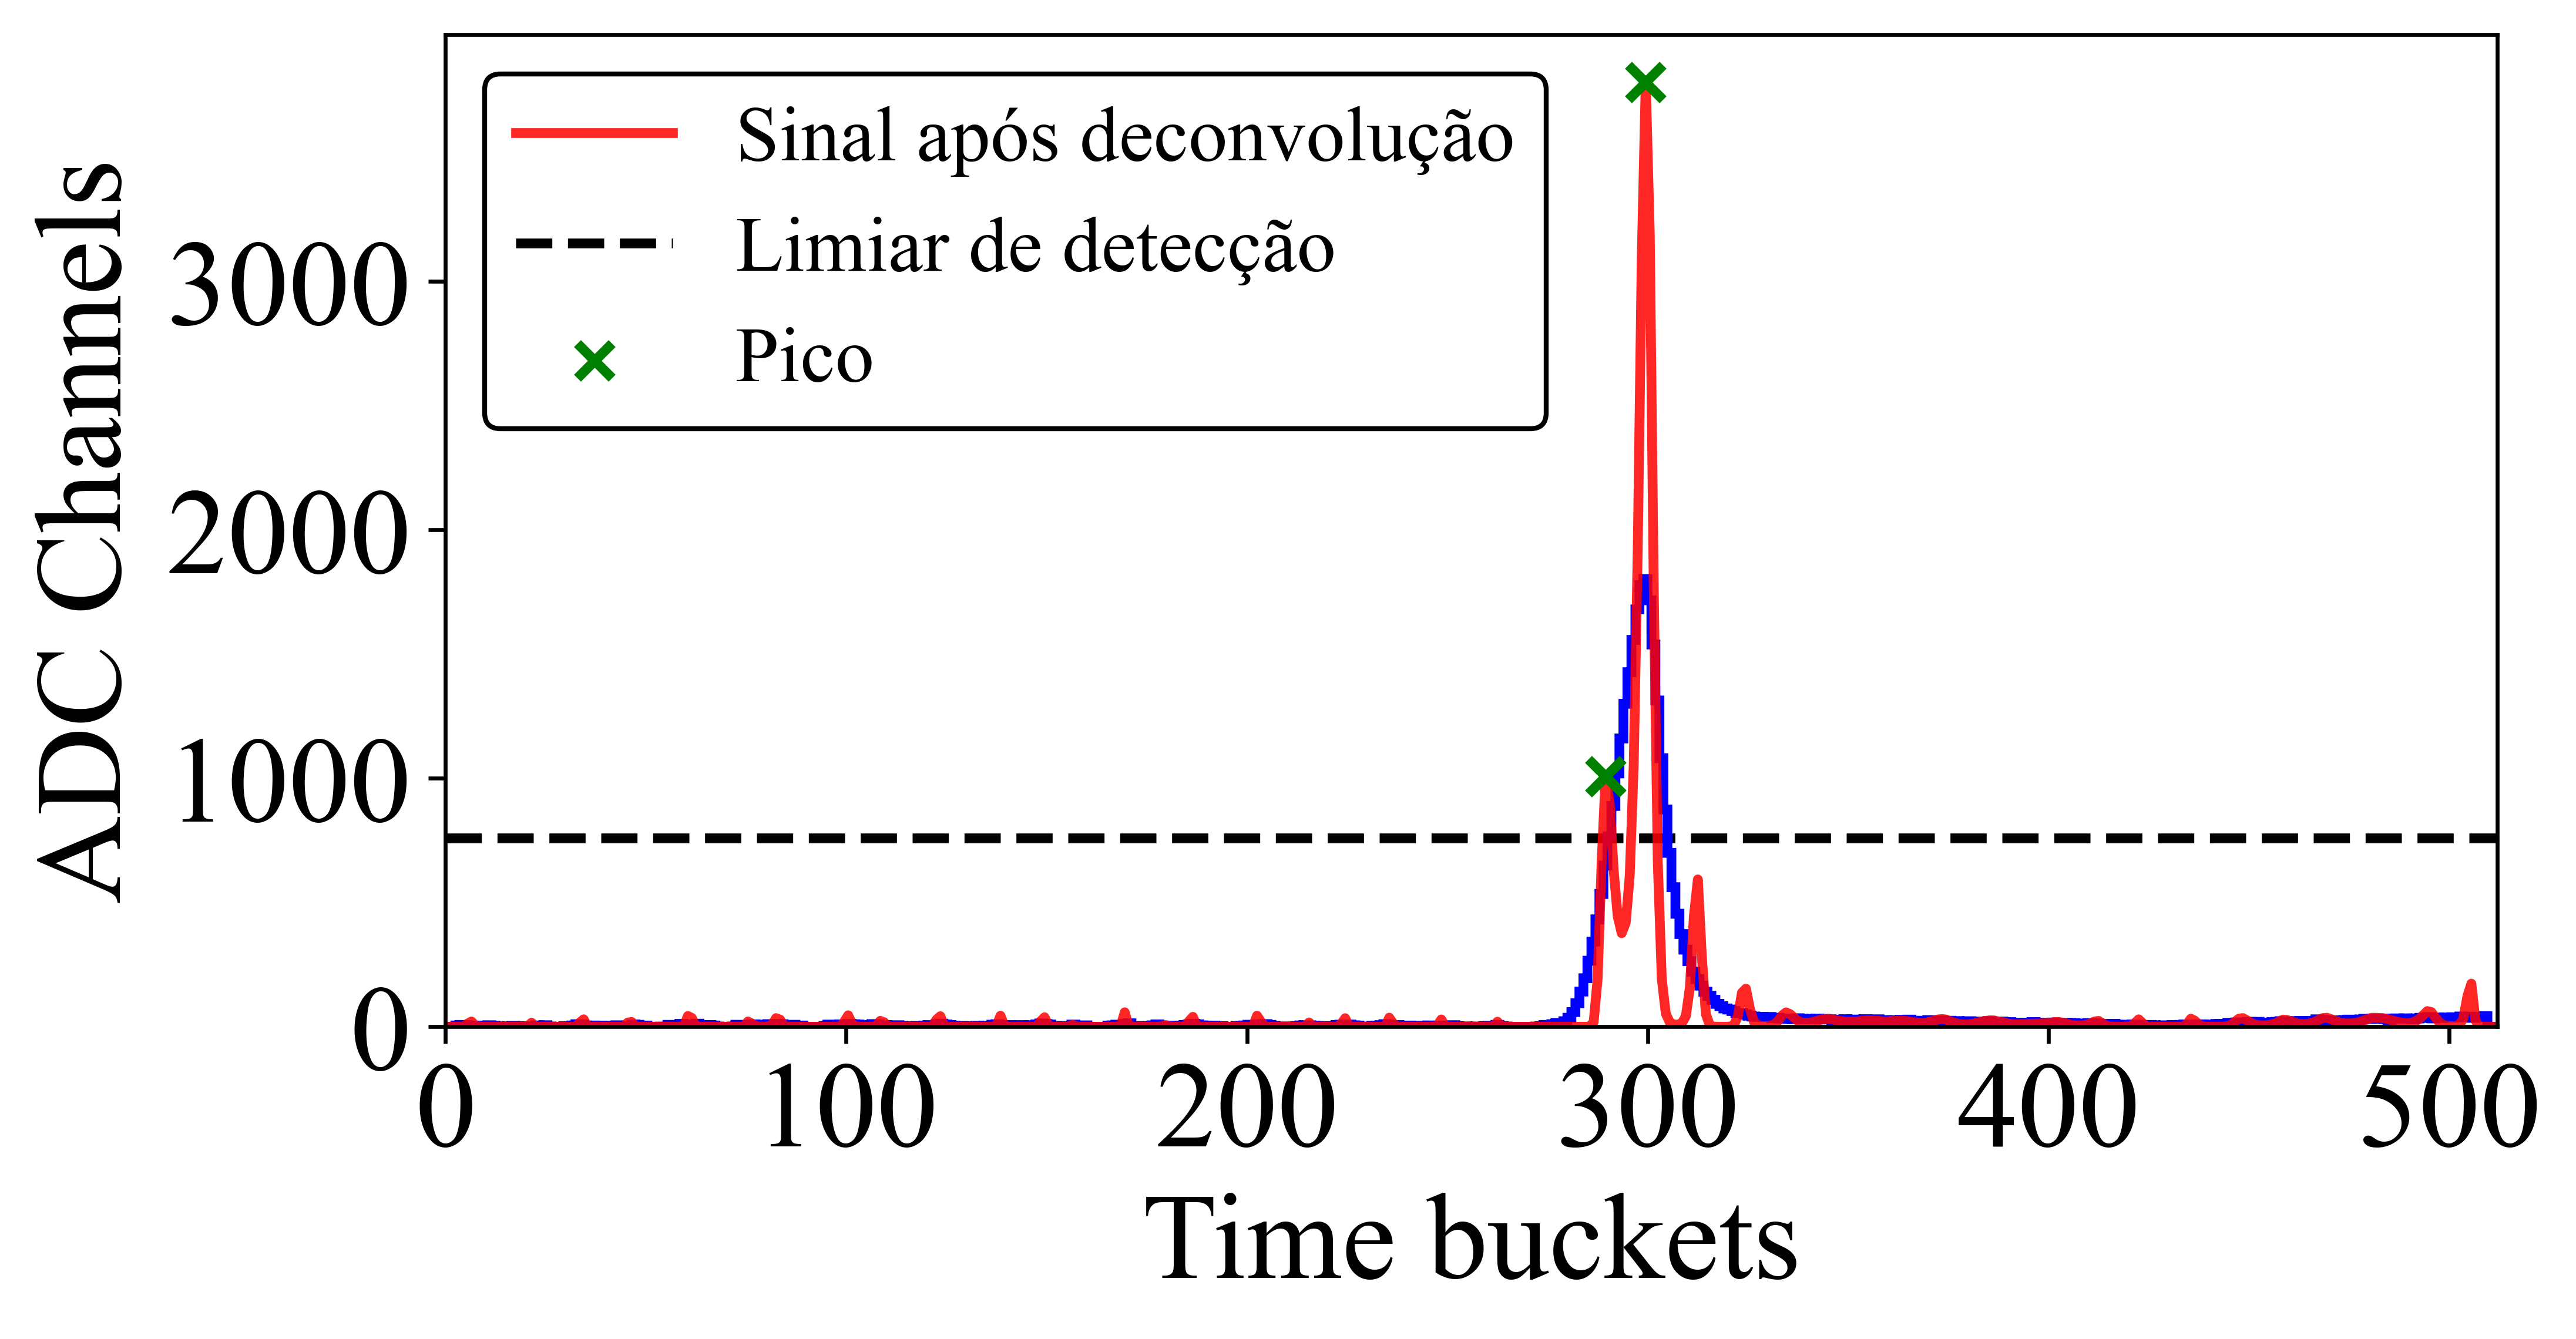
\includegraphics[scale=0.40]{figs/ex_deconv_1.png}
        \caption{}
        \label{subfig:ex_sinal_deconv_1}
    \end{subfigure}%
    \hfill
    \begin{subfigure}[b]{0.48\textwidth}
        \centering
        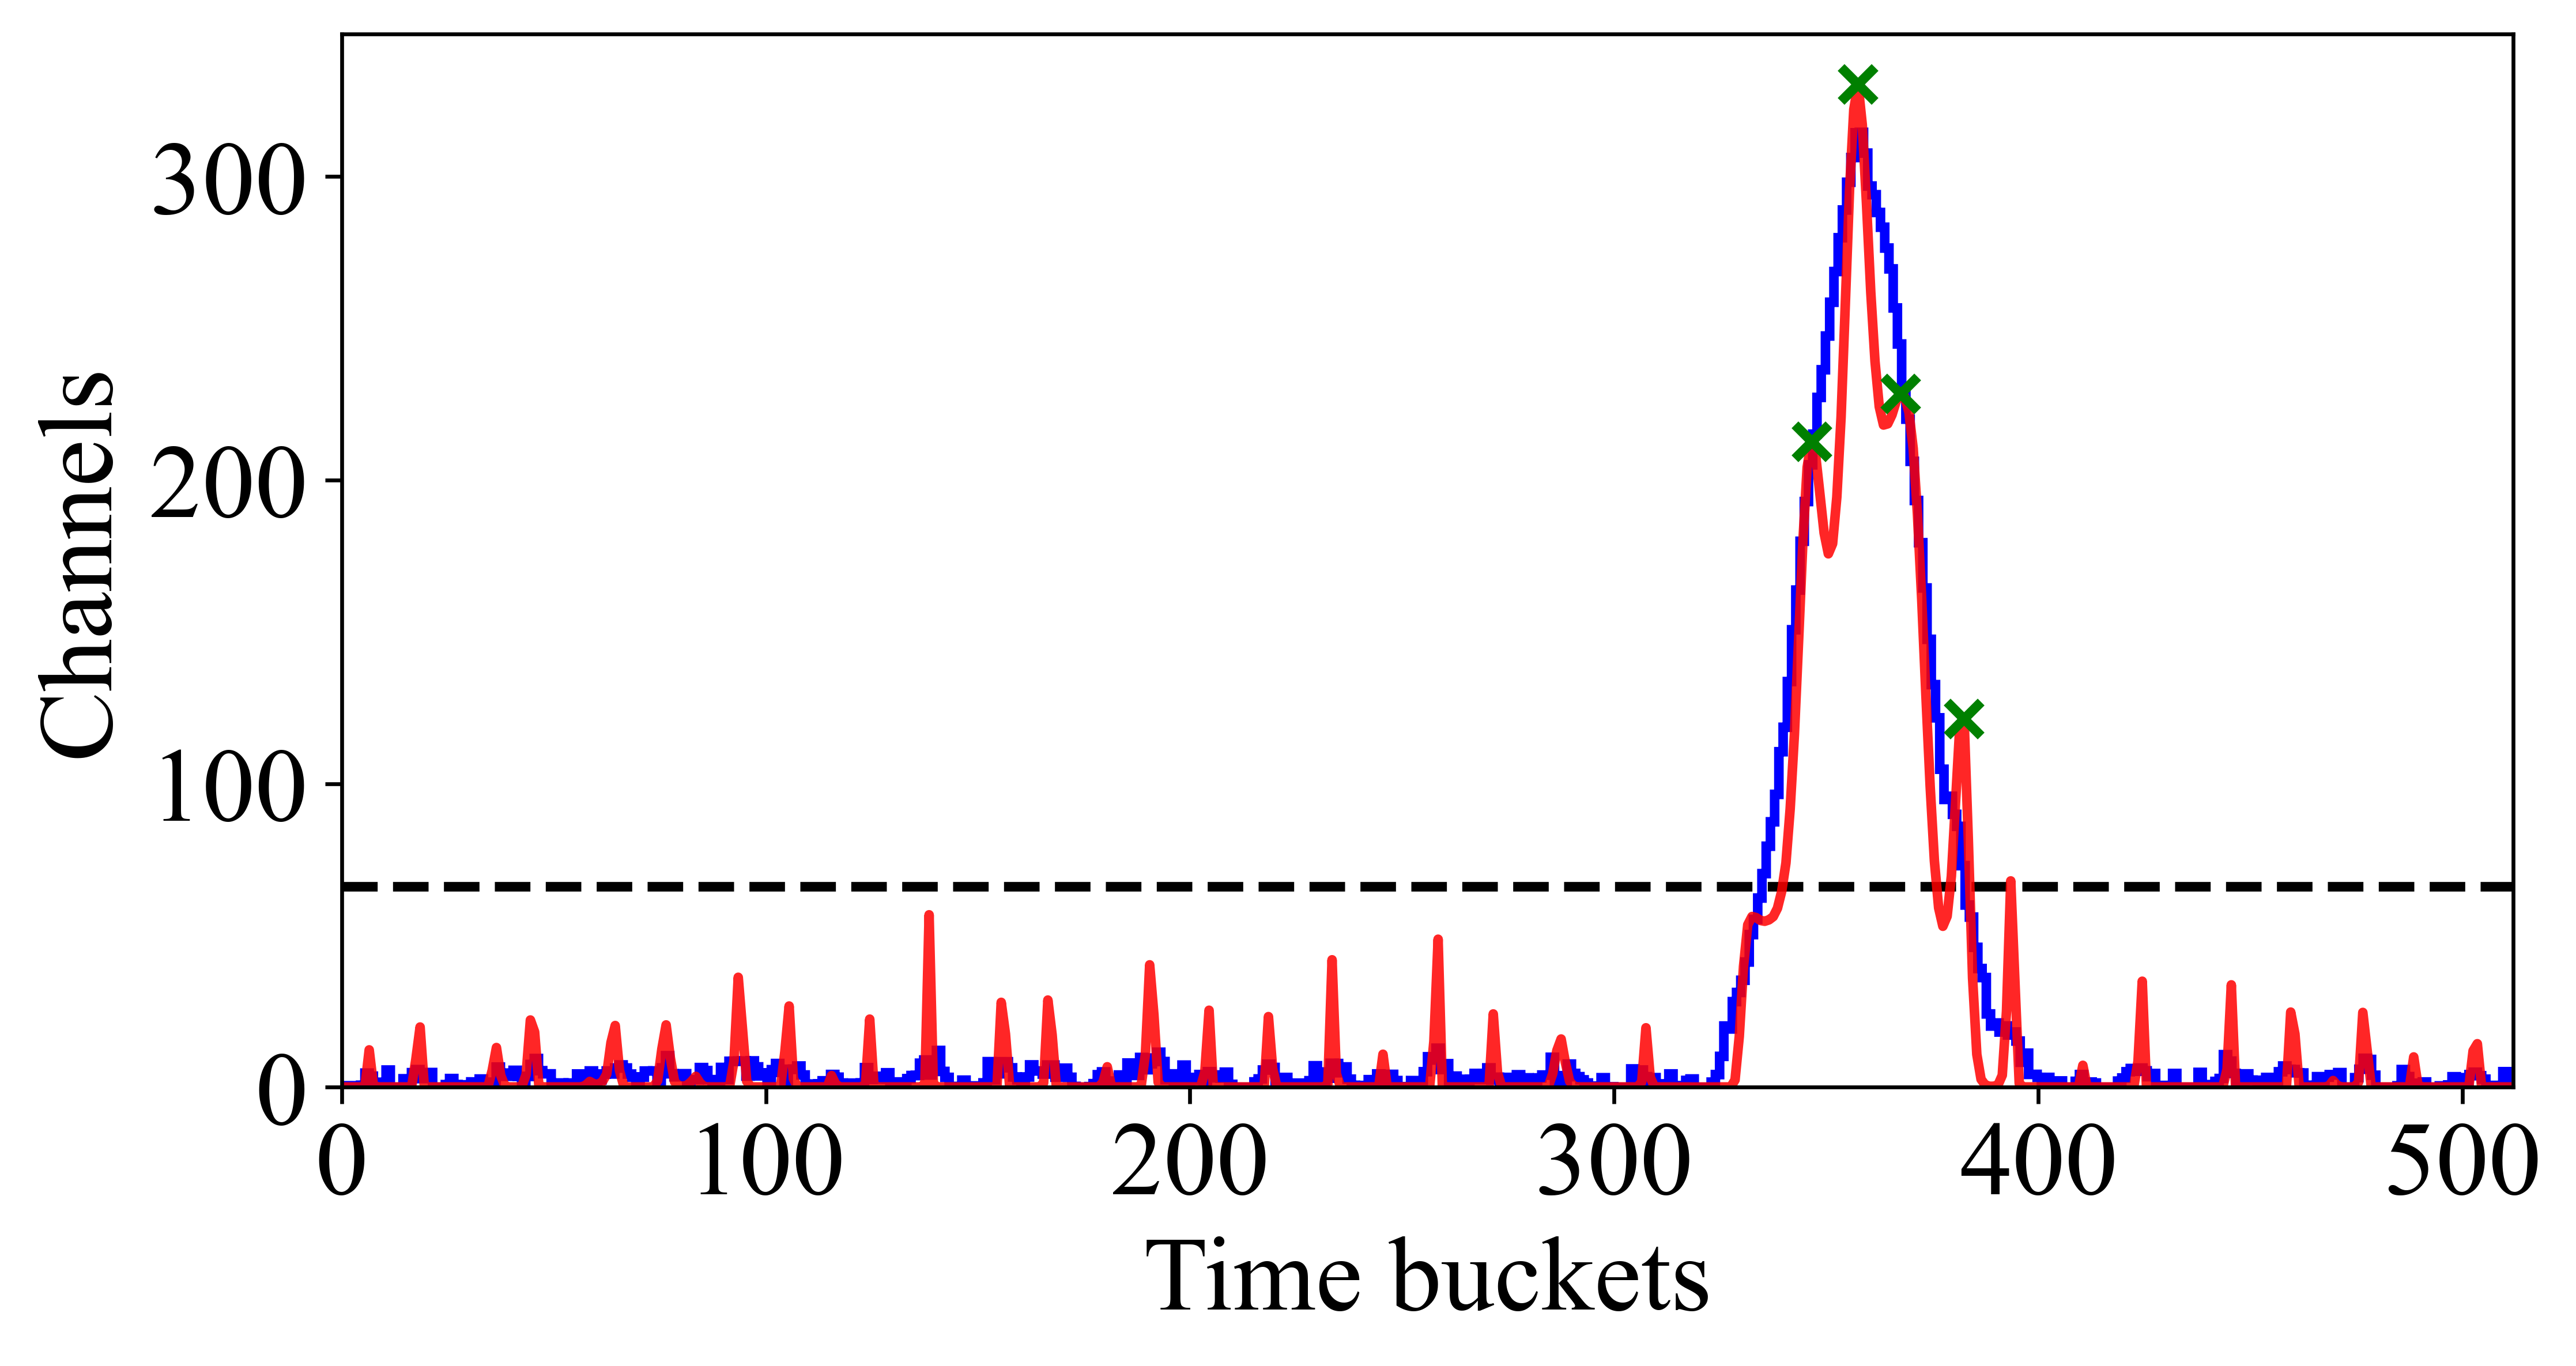
\includegraphics[scale=0.40]{figs/ex_deconv_2.png}
        \caption{}
        \label{subfig:ex_sinal_deconv_2}
    \end{subfigure}
    \begin{subfigure}[b]{0.48\textwidth}
        \centering
        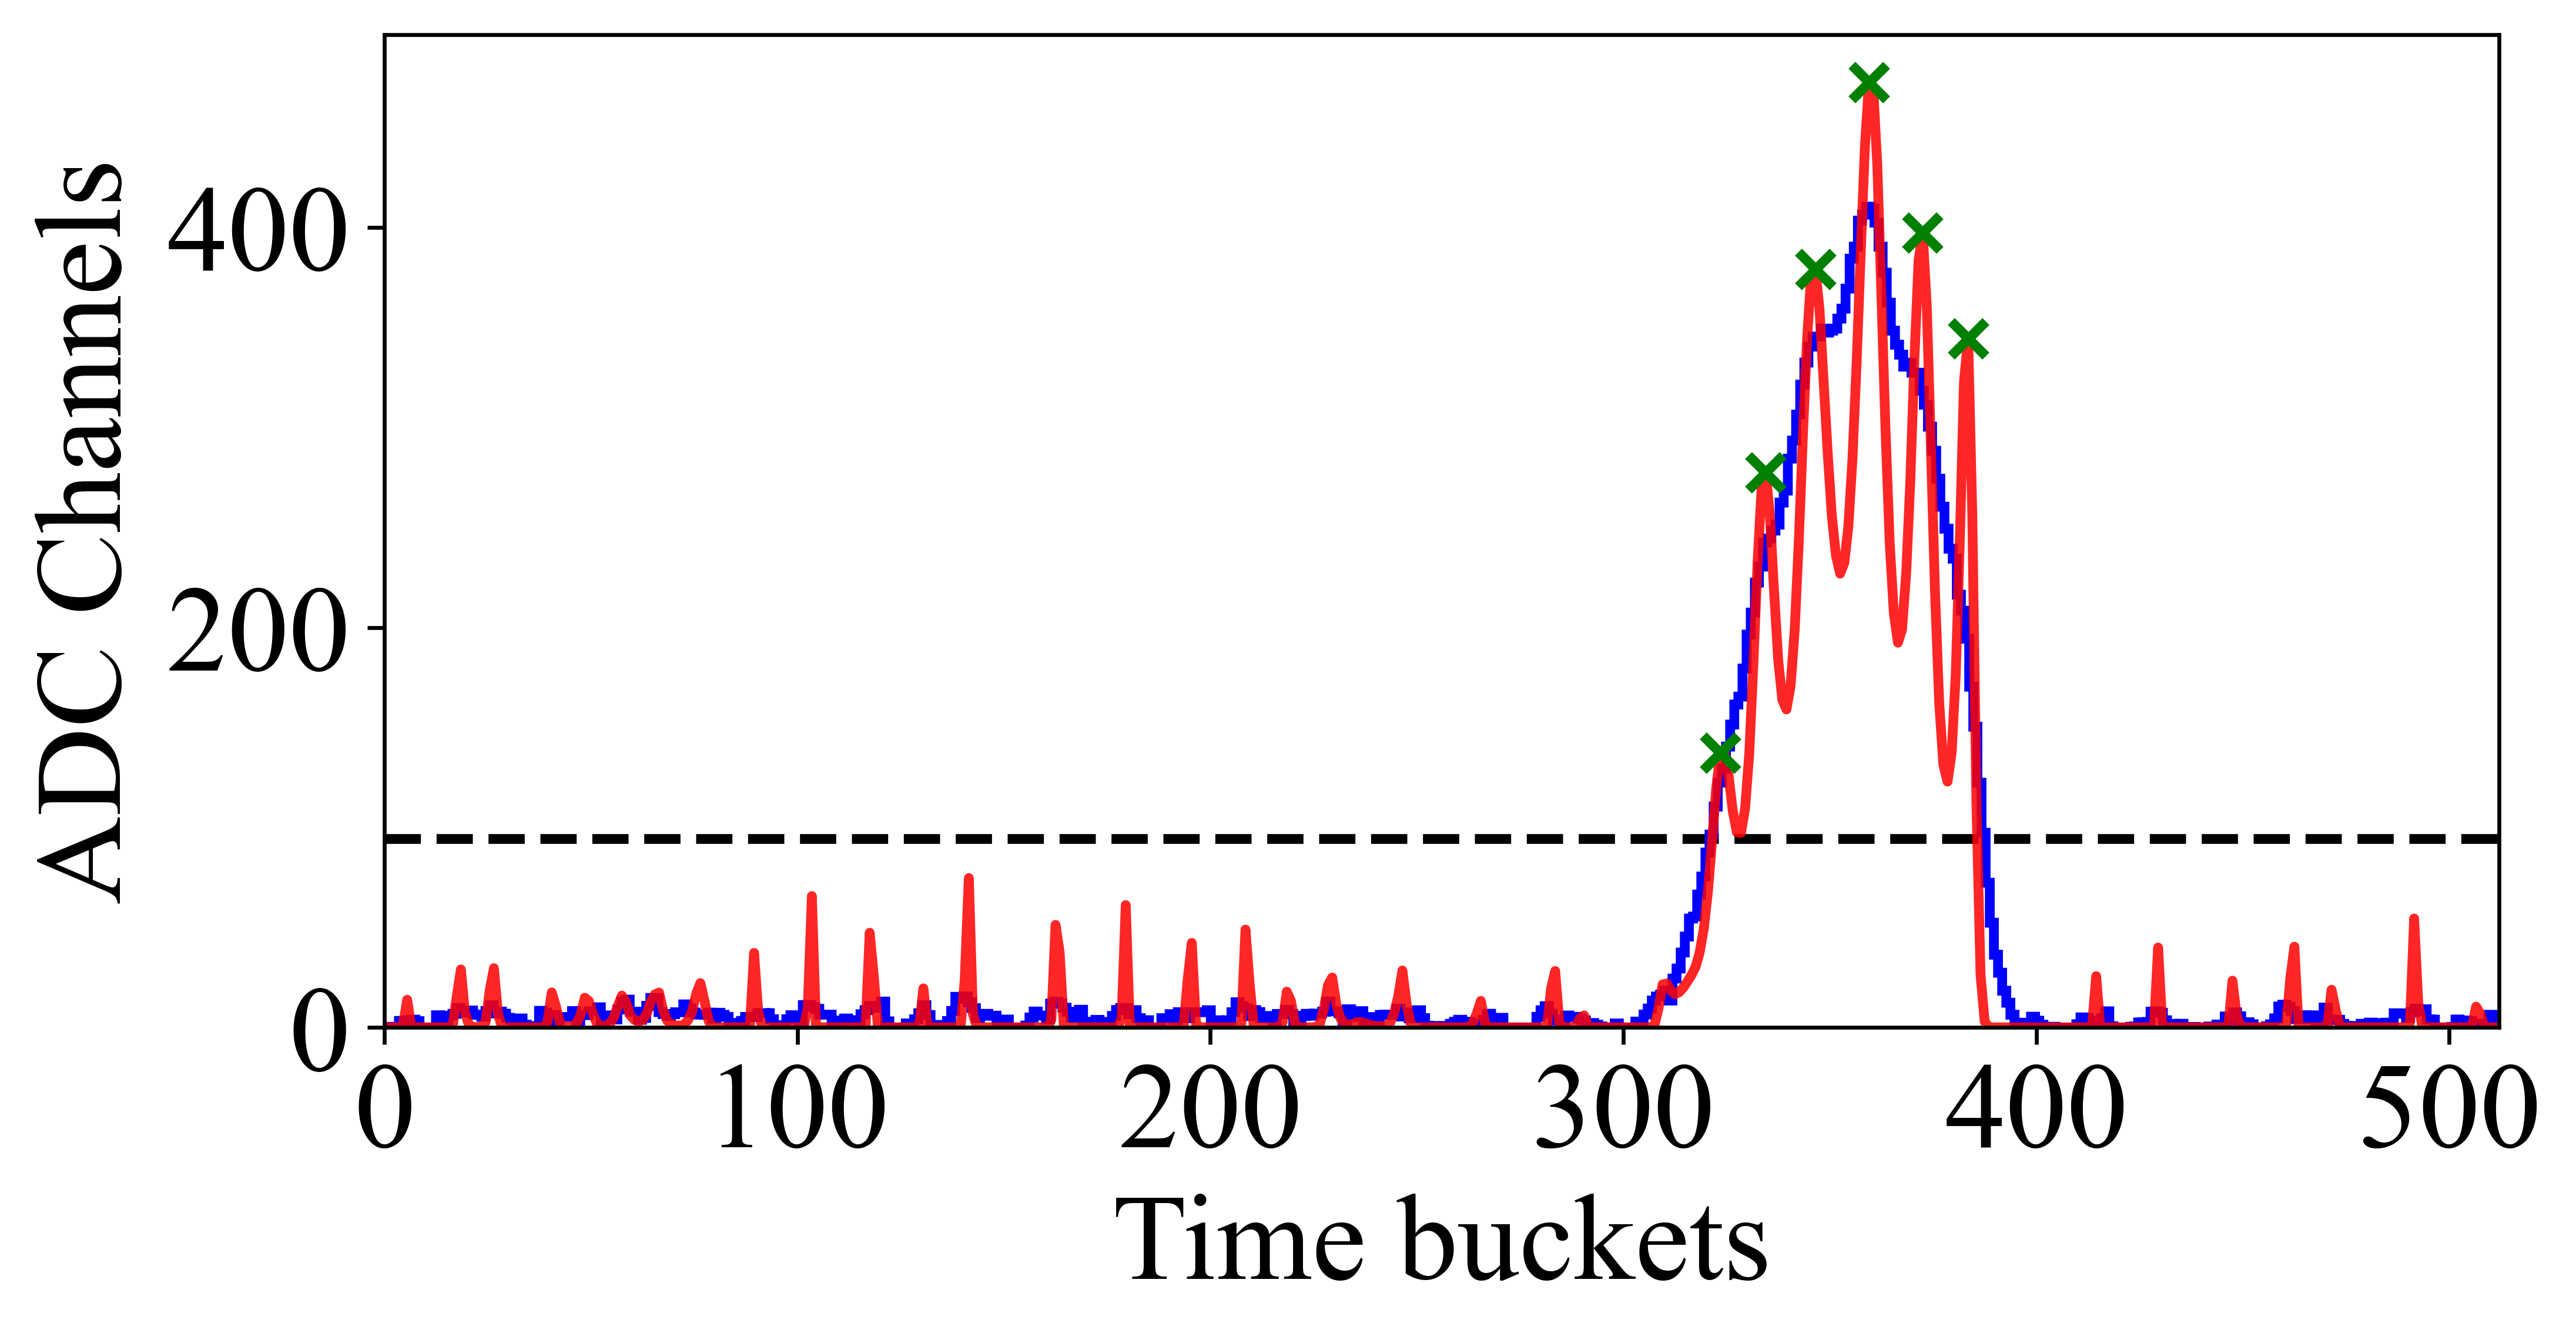
\includegraphics[scale=0.40]{figs/ex_deconv_3.png}
        \caption{}
        \label{subfig:ex_sinal_deconv_3}
    \end{subfigure}%
    \hfill
    \begin{subfigure}[b]{0.48\textwidth}
        \centering
        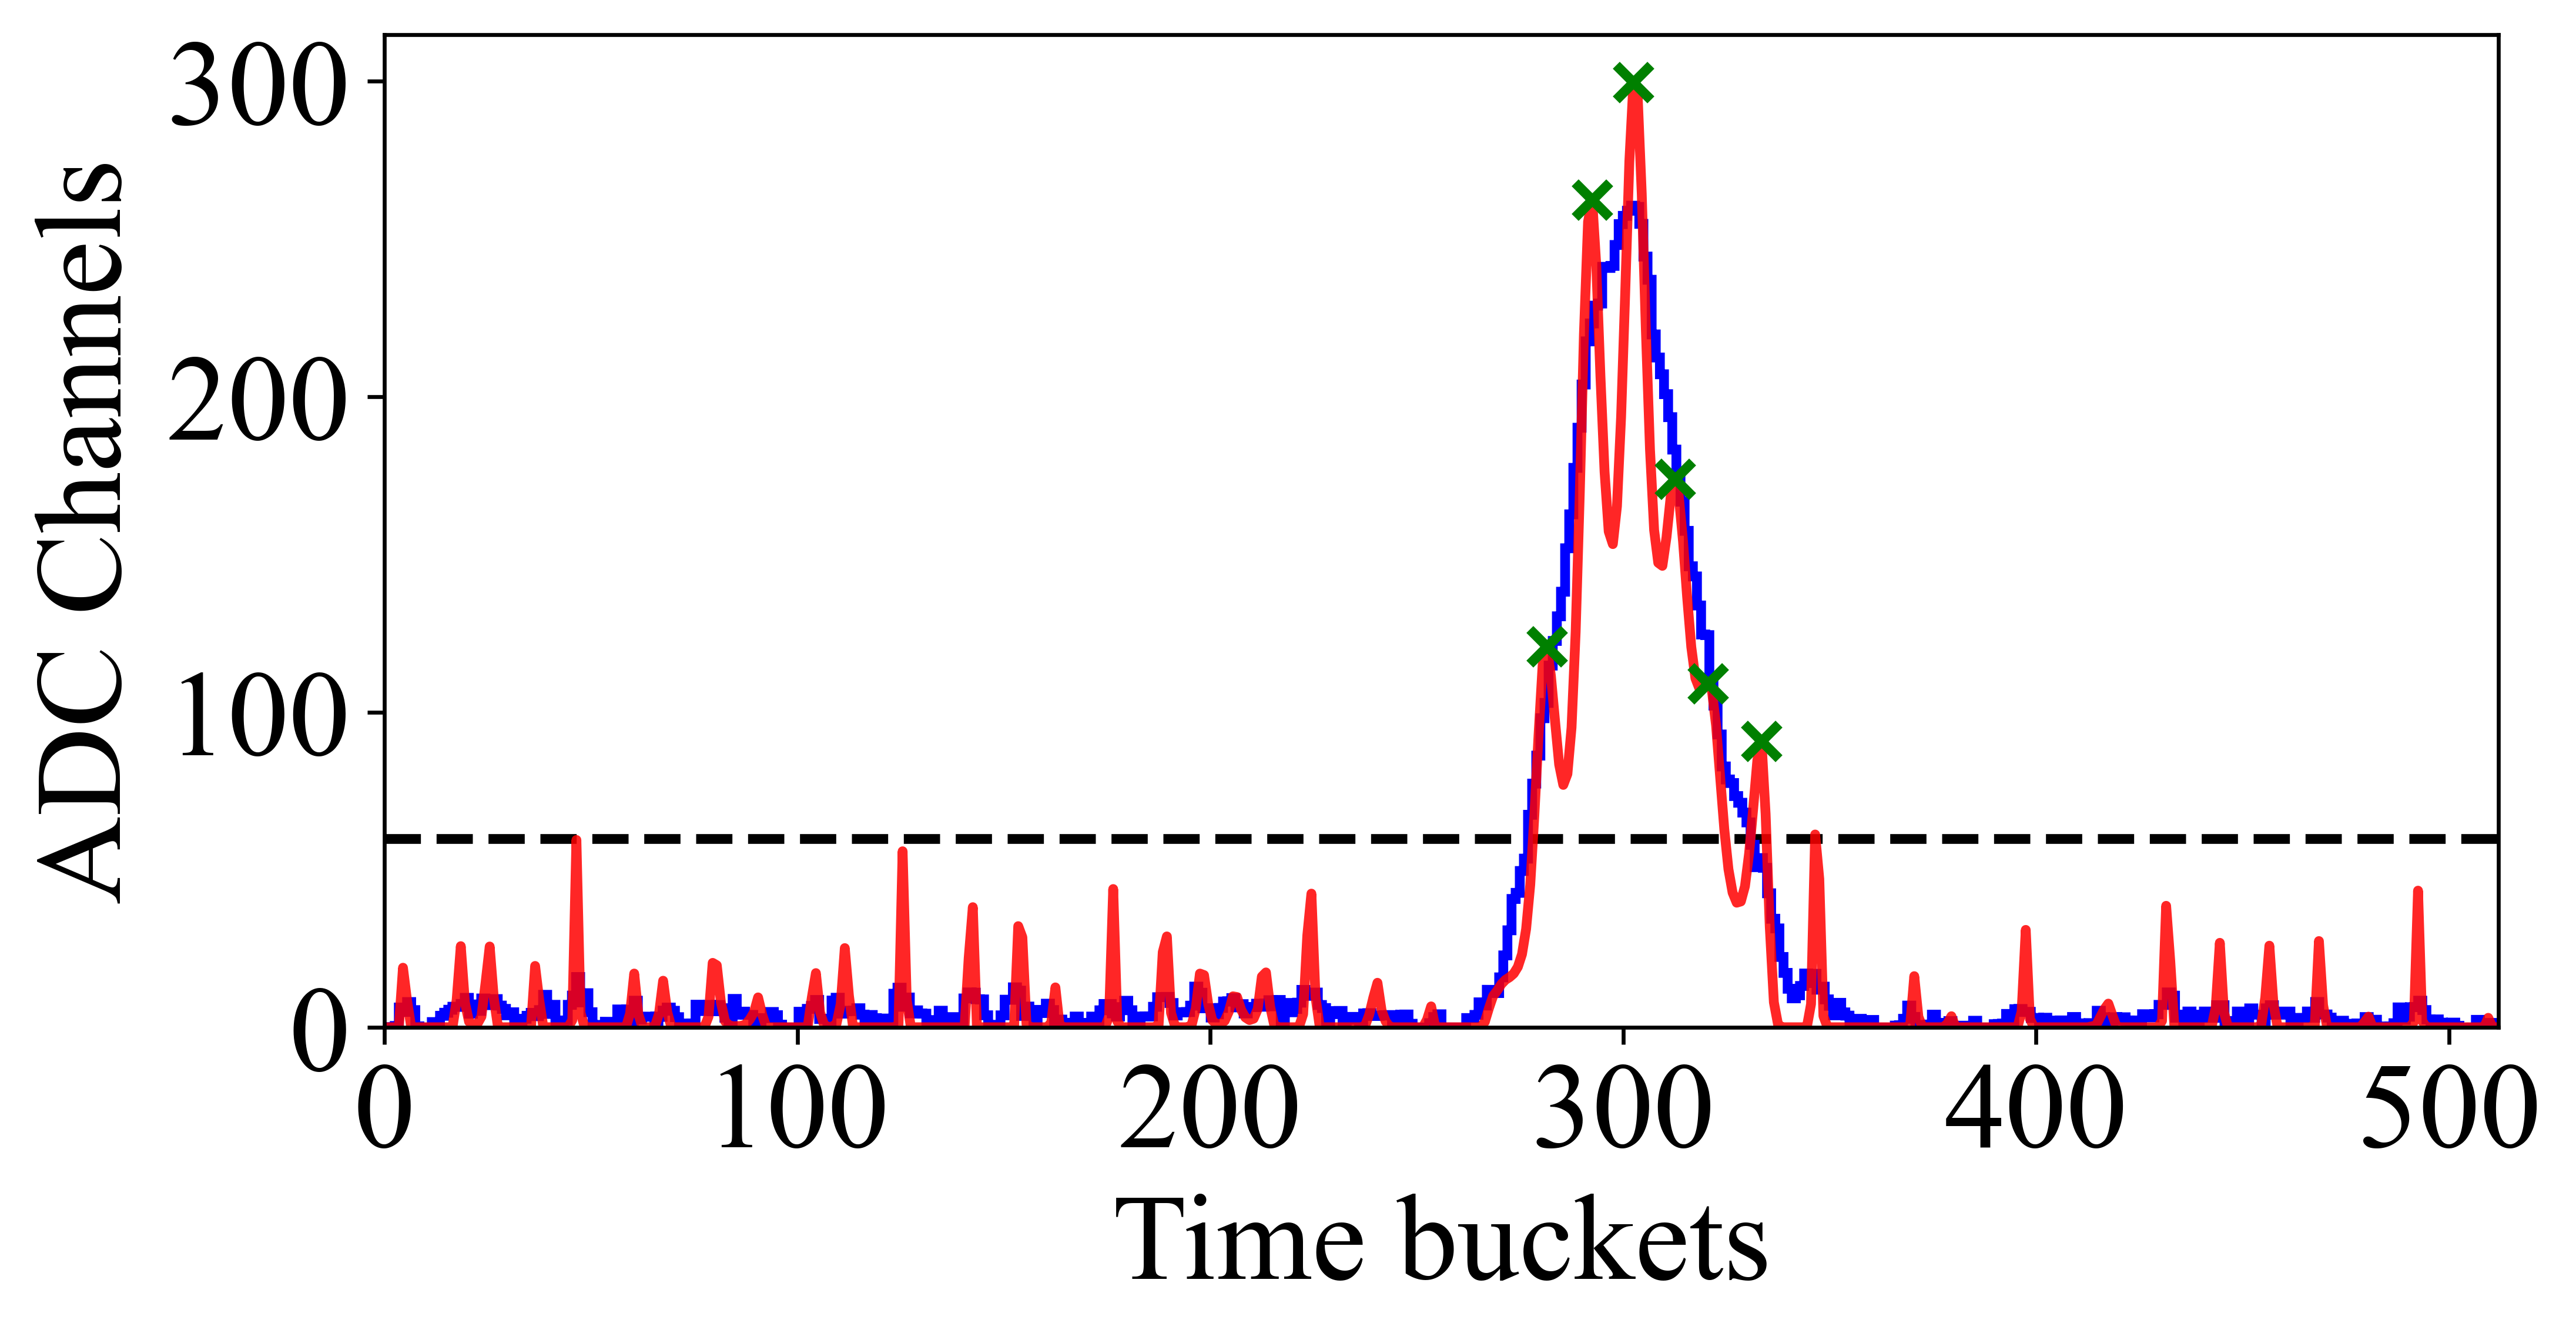
\includegraphics[scale=0.40]{figs/ex_deconv_4.png}
        \caption{}
        \label{subfig:ex_sinal_deconv_4}
    \end{subfigure}
\caption{Histogramas sem as \textit{baselines} antes (em azul) e depois da deconvolução (em vermelho). Os picos (em verde) e o limiar (linha tracejada preta) de identificação também estão indicados.}
\label{fig:ex_sinal_deconv}
\end{figure}

\par O algoritmo de deconvolução também retorna a posição dos centroides encontrados, que indica a localização de um pico. Os mesmo picos podem ser obtidos com o \textit{peak\_finder}, com a vantagem de que o algoritmo possui muitos parâmetros diferentes para calibração, melhorando a identificação em comparação com os picos identificados pelo algoritmo do TSpectrum. A execução de 200.000 sinais, desde a estimativa e remoção do fundo, até a identificação dos centroides, demora cerca de 23.25 minutos, usando o processador Ryzen 5 3600X.

\par Para determinar a carga acumulada $Q$ de cada ponto, é necessário calcular a área do centroide do pico identificado. A área do sinal antes e depois da deconvolução é a mesma, mesmo para a região dos pulsos, portanto pode-se analisar diretamente o sinal após a deconvolução. Para achar a área do pulso, foi calculada a largura dos pulsos após a deconvolução, para determinar a área como uma simples integral gaussiana. O sigma dos pulsos após a deconvolução é $\sigma_{dd}$ = 1.1543 (44) \textit{time buckets}. Com isso foi calculada a carga acumulada para cada ponto descoberto do evento. A carga acumulada $Q$ para cada ponto $i$ é dada por:

\begin{equation}\label{eq:gauss_area}
    Q = \int^\infty _{-\infty} Ae^{-(t' - t_i)^2 / 2\sigma_{dd}^2} dt' = A\left |\sigma_{dd} \right|\sqrt{2\pi},
\end{equation}

\par onde $A$ é a amplitude do ponto com centroide $t_i$ e desvio padrão após a deconvolução $\sigma_{dd}$.

\par Com o banco de dados para a deconvolução e também para a identificação de picos, basta criar as redes neurais, que serão descritas na seção \ref{sec:pulsos_ml}.

\section{Análise dos pulsos com \textit{machine learning}}\label{sec:pulsos_ml}


\par Com \textit{machine learning} temos a possibilidade de criar algoritmos de alta complexidade sem definir operações explícitas. Usando os resultados das seções anteriores foram desenvolvidas três redes neurais, com o objetivo de: estimar o fundo (subseção \ref{subsec:pulso_ml_fundo}), fazer a deconvolução (\ref{subsec:pulso_ml_deconv}) e por fim identificar os picos (subseção \ref{subsec:pulso_ml_peaks}). 

%Os resultados dos algoritmos usados nas subseções \ref{subsec:pulses_baseline} e \ref{subsec:pulses_deconv} foram usados como \textit{outputs} para o aprendizado das redes neurais que foram desenvolvidas em cada etapa.

\subsection{Rede neural para o fundo}\label{subsec:pulso_ml_fundo}

\par O objetivo foi criar uma rede neural que reproduza o comportamento do algoritmo \textit{background removal} que estima o fundo do sinal, que foi discutido na seção \ref{subsec:pulses_baseline}, tentando reproduzir resultados muito similares. A rede neural neural é supervisionada, onde os dados de entrada são os sinais brutos e as saídas devem ser os fundos de cada sinal. A arquitetura está na figura \ref{fig:arq_source_to_bkg}.

% \par Estimar o fundo é uma tarefa muito complexa pois a eletrônica do detector faz com que o sinal do canal varie muito dependendo do evento, podendo muitas vezes fazer com que o fundo tenha saltos no espectro após receber o sinal de um pulso. Importante ressaltar que a retirada do fundo não precisa ser considerada perfeita. O próprio algoritmo analítico de remoção de fundo não é perfeito e no geral nunca coloca toda a parte que não é o pulso em 0, há muitas flutuações. O importante é tentar deixar o mais próximo de zero possível. 

% \par Estimar o fundo é uma tarefa muito complexa pois ele não é analítico, podendo muitas vezes fazer com que o fundo tenha saltos em diferentes \textit{time buckets}. 

\begin{figure}[H]
    \centering
    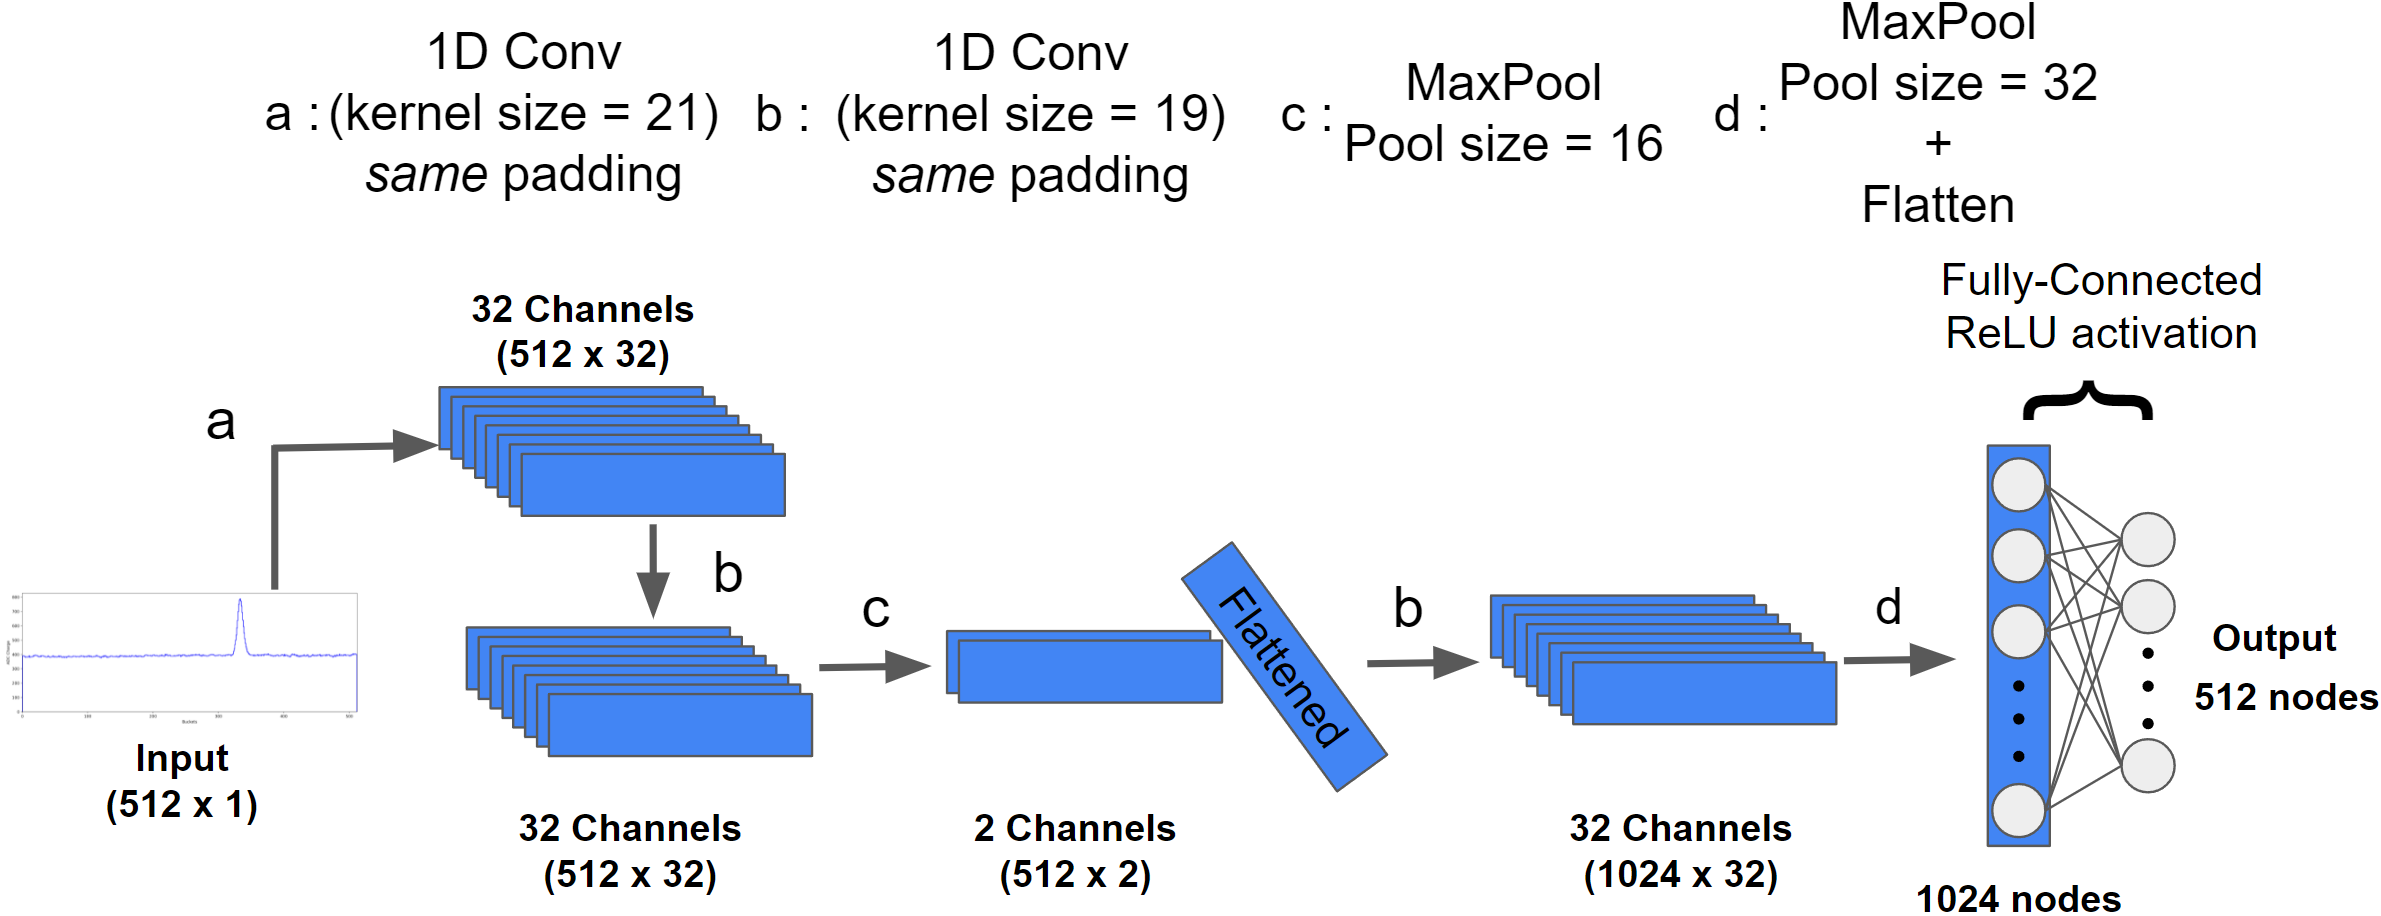
\includegraphics[scale = 0.238]{figs/Source to only bkg.png}
    \caption{Arquitetura da rede neural que faz a inferência do fundo. O vetor de entrada deve ter dimensionalidade 512 x 1. Todas as partes com convolução não possuem o parâmetro \textit{bias}.}
    \label{fig:arq_source_to_bkg}
\end{figure}

\par A entrada da rede é o sinal cru com dimensionalidade 521 x 1. Há duas convoluções seguidas (passagens \textit{a} e \textit{b}) com \textit{padding same}, seguida de uma camada com \textit{Max pooling}. Os dois canais restantes sofrem uma planificação (ou \textit{flat}), diminuindo sua dimensionalidade, para então passar por mais uma convolução com \textit{padding same} e filtros de tamanho 19 seguido de uma camada \textit{Max pooling} e uma camada \textit{Fully Connected} com função de ativação \textit{ReLU}. Toda a rede neural foi construída usando o TensorFlow 2 e possui um total de 545.536 parâmetros, todos treináveis. O tamanho dos filtros das convoluções levam em conta a largura do pulso, sendo no mínimo maior que a largura, a fim de que cada \textit{kernel} atue em um pulso completo na convolução \cite{FORTINO2022166497}.

\par A camada final com função de ativação \textit{ReLU} garante o valor mínimo de saída em 0 e, principalmente, pelo fato de não causar problemas à minimização do gradiente \cite{VGP}. Foram testadas diversas combinações e a mostrada na figura \ref{fig:arq_source_to_bkg} é a que obteve os melhores resultados \cite{FORTINO2022166497}. 
% Caso, por exemplo, na passagem \textit{c} da figura, o \textit{pool size} da camada de \textit{max pooling} fosse 32 (a fim de sobrarem 512 canais igual na entrada e na saída), a rede parece não entender as oscilações grandes do sinal de fundo.

\par Para o treino foram usados 160.000 sinais para treino e 40.000 para validação. O \textit{loss} foi escolhido como sendo o erro quadrático médio (equação \ref{eq:erro_abs_m}, o otimizador foi o \textit{ADAMAX} \cite{ADAMAX}, com \textit{learning rate} de 0.0005, e métrica para avaliação foi o erro médio absoluto, dado por

\begin{equation}\label{eq:erro_abs_m}
    E = \frac{1}{N}\sum_{i = 1}^{N} \left | x_i - \Hat{x}_i\right |,
\end{equation}

onde $E$ é o erro absoluto médio, $N$ é o número de pontos e $x_i$ o ponto da saída da rede para ser comparado com o ponto original $\Hat{x}_i$. Foram 30 \textit{epochs} e o \textit{batch-size} foi 8. O treino foi realizado no Google Colaboratory \cite{google_colab} usando a GPU (\textit{graphics processing unit}) NVIDIA Tesla P100 e durou cerca de 34 minutos. Os resultados do treino estão na figura \ref{fig:source_to_bkg_results}.

% \par Como dito na seção \ref{sec:ml} temos que especificar qual o tamanho do filtro das camadas convolucionais. Para determinar o fundo precisamos, ponto a ponto, determinar quantos canais na direita e na esquerda o filtro deve atuar. Por exemplo, caso o tamanho do filtro fosse 3, ele só estaria ``enxergando" um ponto à direita e um à esquerda, para então passar a informação a diante, porém claramente é um filtro muito pequeno, as oscilações podem variar mais do que 5 canais. Além disso, quando há o começo de um pulso no sinal, ele pode se estender por múltiplos canais, então é preciso escolher um tamanho de filtro grande o suficiente para enxergar todas essas diferenças. A rede consta com duas camadas convolucionais em sequência com filtros de tamanho 21 e 19, respectivamente.

\begin{figure}[H]
\centering
    \begin{subfigure}[t]{\textwidth}
        \centering
        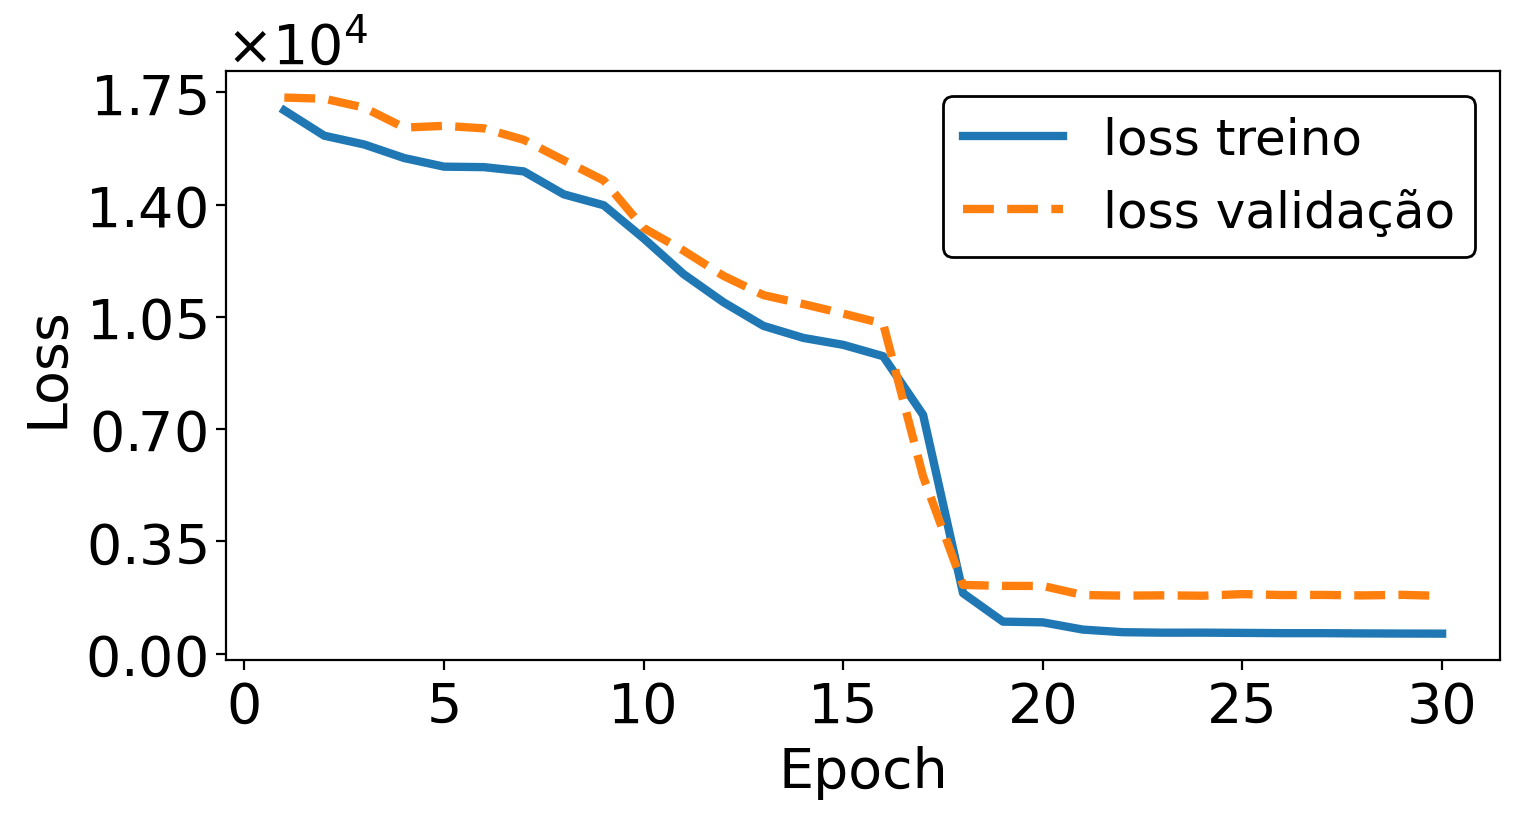
\includegraphics[scale=0.51]{figs/source_to_bkg_loss.png}
        \caption{\textit{Loss} dos dados de treino (linha contínua) e dos dados de validação (linha tracejada) em função da \textit{epoch} no treino da rede dada pela figura \ref{fig:arq_source_to_bkg}.}
        \label{subfig:source_to_bkg_loss}
    \end{subfigure}%
    \vfill
    \begin{subfigure}[t]{\textwidth}
        \centering
        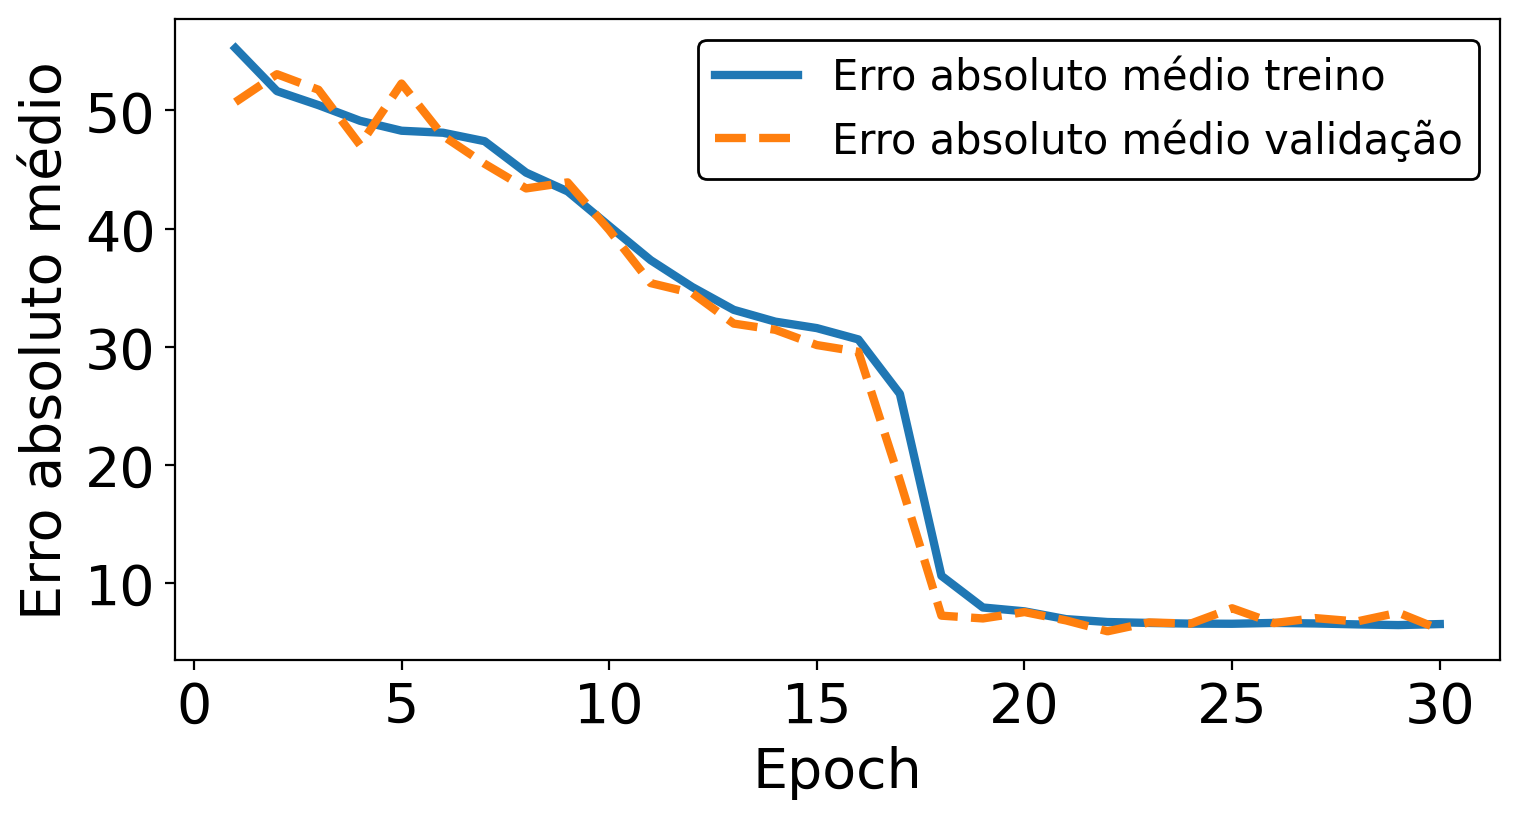
\includegraphics[scale=0.51]{figs/source_to_bkg_metric.png}
        \caption{Erro absoluto médio dos dados de treino (linha contínua) e dos dados de validação (linha tracejada) em função da \textit{epoch} no treino da rede dada pela figura \ref{fig:arq_source_to_bkg}.}
        \label{subfig:source_to_bkg_metric}
    \end{subfigure}
\caption{Resultados do treino da rede neural dada pela figura \ref{fig:arq_source_to_bkg}. A rede atingiu seu melhor resultado a partir da \textit{epoch} 20 aproximadamente, quando começa um 
platô no \textit{loss}.}
\label{fig:source_to_bkg_results}
\end{figure}

% \par A métrica do erro absoluto médio mede ponto a ponto qual o erro absoluto da previsão. 

\par A arquitetura da figura \ref{fig:arq_source_to_bkg} (assim como as próximas desse capítulo) foi determinada de forma empírica. Uma arquitetura com menos passagens e/ou menos parâmetros fornece resultados menos adequados em comparação com a arquitetura apresentada. No caso de mais parâmetros e /ou passagens (consequentemente com aumento no tempo de execução), a rede neural não demonstrou melhora substancial.

\par Exemplos de resultados de previsões da rede neural estão na figura \ref{fig:stb_examples}. A previsão do fundo possui um erro absoluto nos dados de treino de 6.5315 ADC Channels e nos dados de validação de 6.0783 ADC Channels. O sinal cru é subtraído do fundo, colocando o valor mínimo da subtração em 0. Comparando o erro médio absoluto de 200.000 sinais sem o respectivo fundo (resultante do algoritmo do TSpectrum) com o resultado da rede neural obtemos 4.5 ADC Channels.
% Esse erro significa que, por exemplo, para o menor pico detectado considerado, que possui amplitude de cerca de 60 unidades em y, a incerteza estimada da amplitude seria de 7.5\%, ou seja, na menor amplitude possível para um pico a incerteza propagada seria de 7.5\% da amplitude.

\par Rede neurais convolucionais têm a vantagem de usarem poucas variáveis e serem facilmente paralelizadas em sua execução \cite{mlbook}. Uma vantagem de redes neurais é o seu tempo de execução. Empiricamente a rede neural pode processar 200.000 sinais em apenas 8s (ou 25.000 sinais por segundo), sendo muito eficiente em tempo.

\begin{figure}[H]
\centering
    \begin{subfigure}[b]{0.47\textwidth}
        \centering
        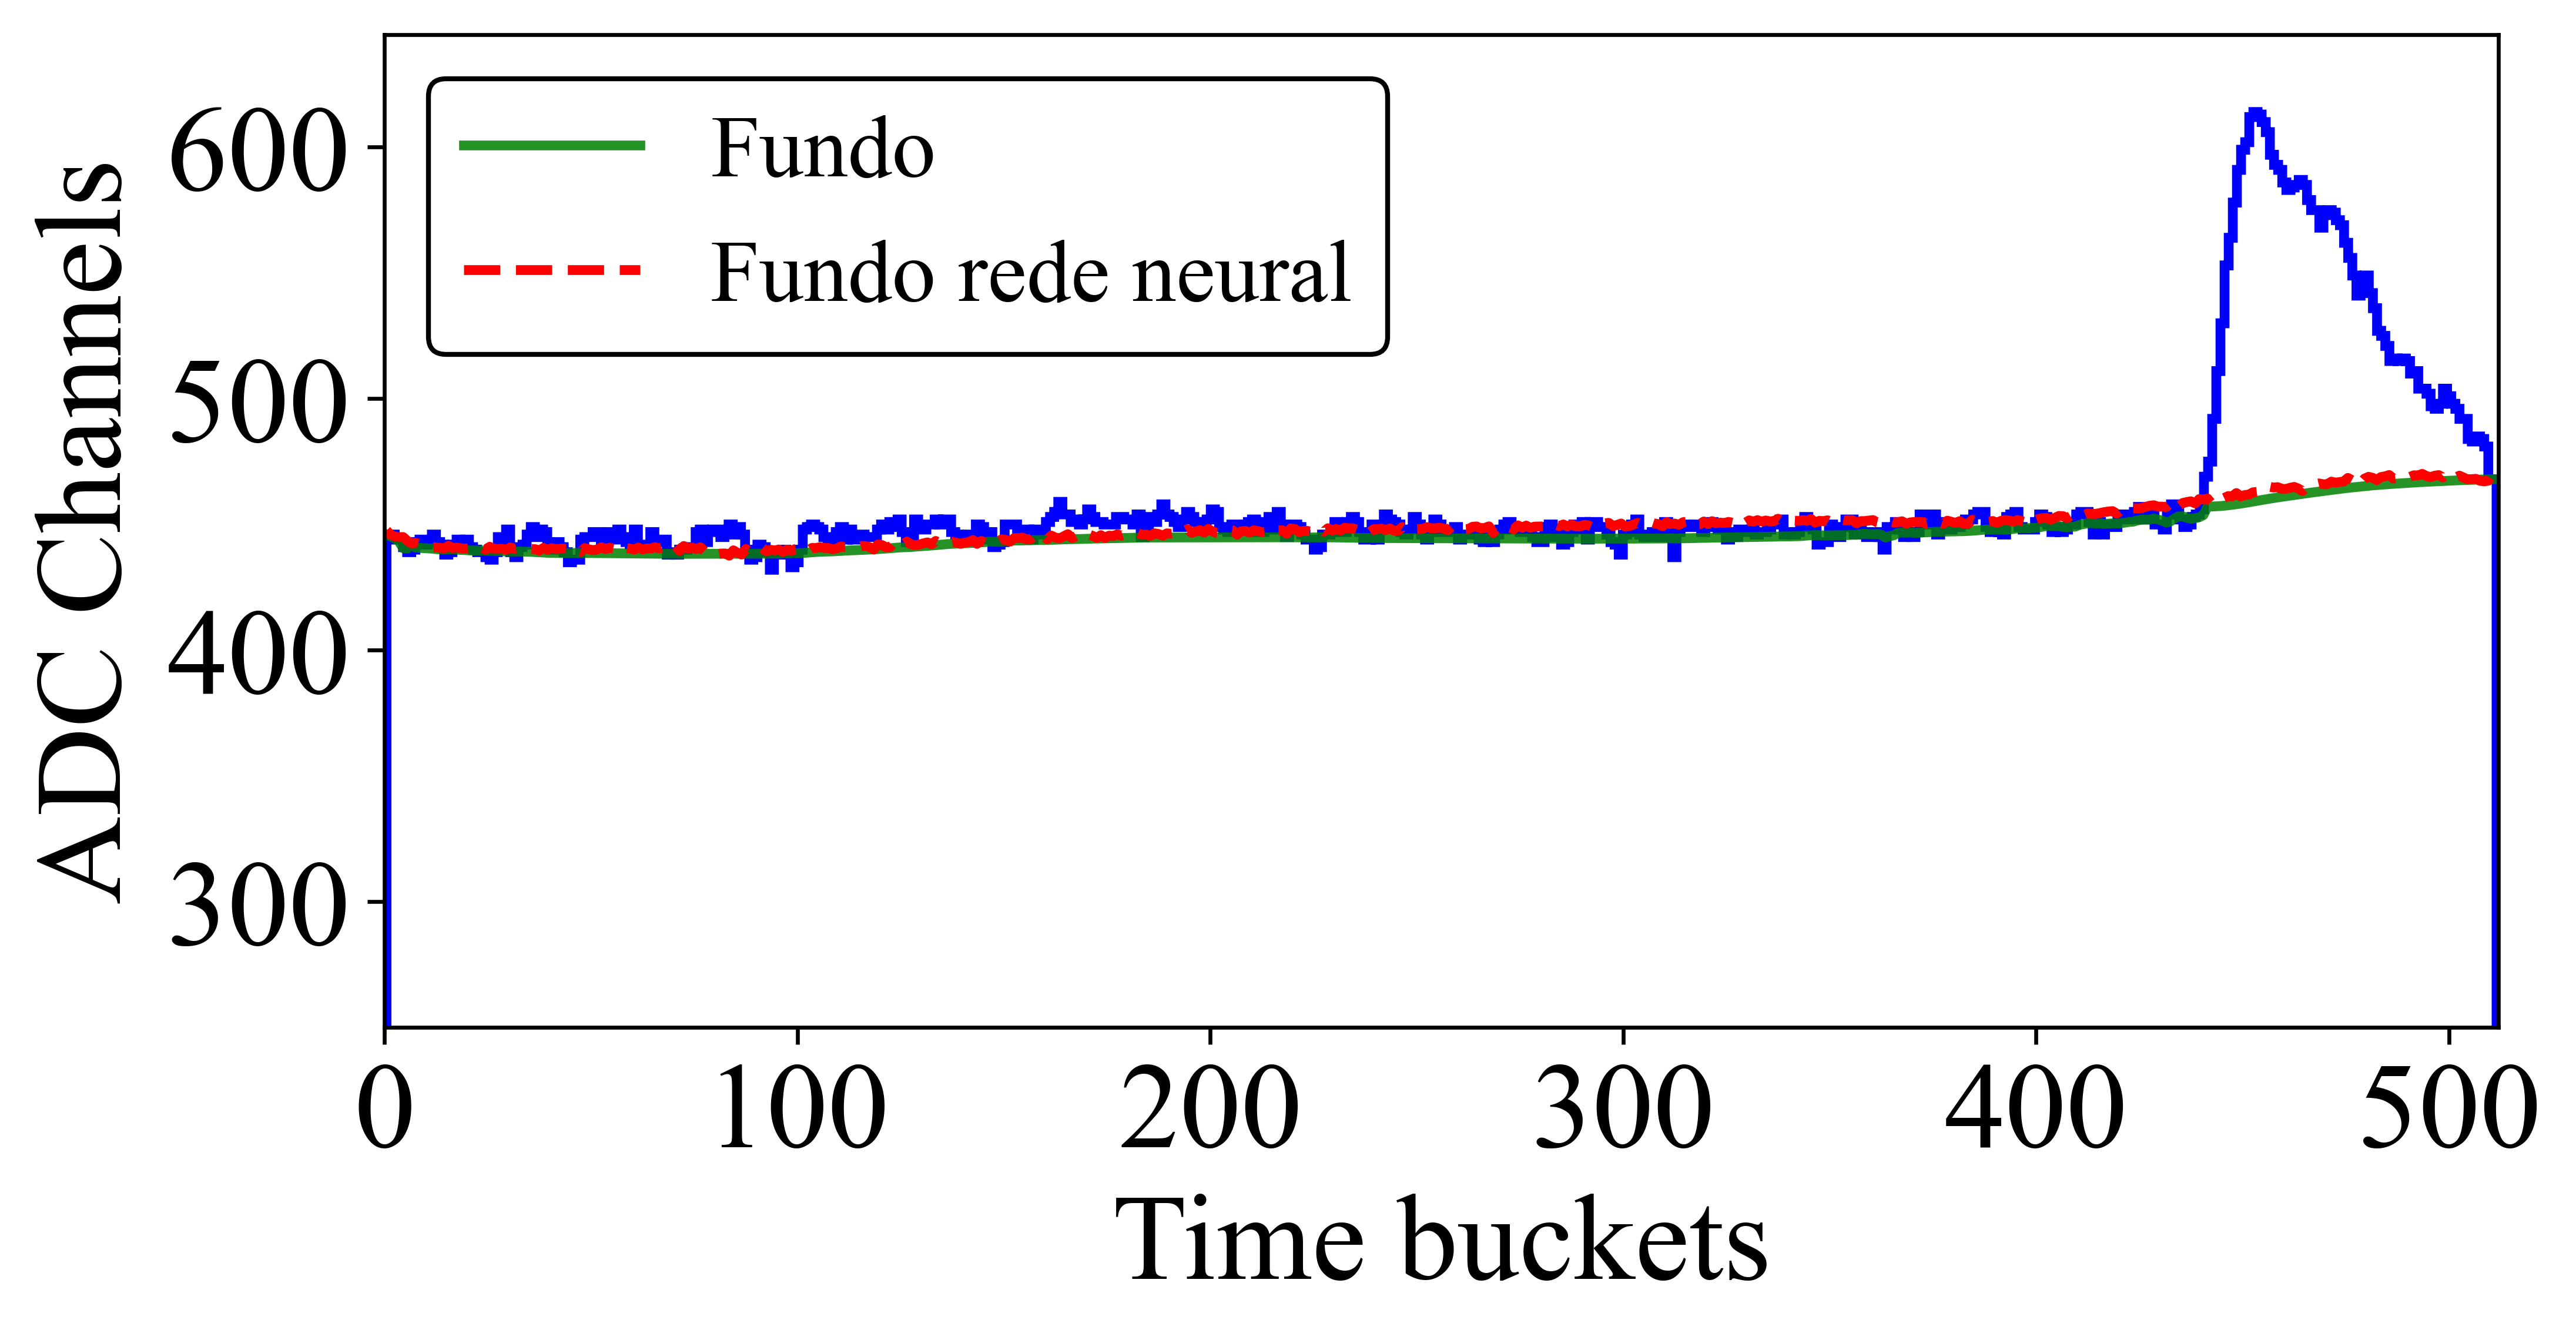
\includegraphics[scale=0.43]{figs/stb_1.png}
        \caption{}
        \label{subfig:stb_ex1}
    \end{subfigure}%
    \hfill
    \begin{subfigure}[b]{0.46\textwidth}
        \centering
        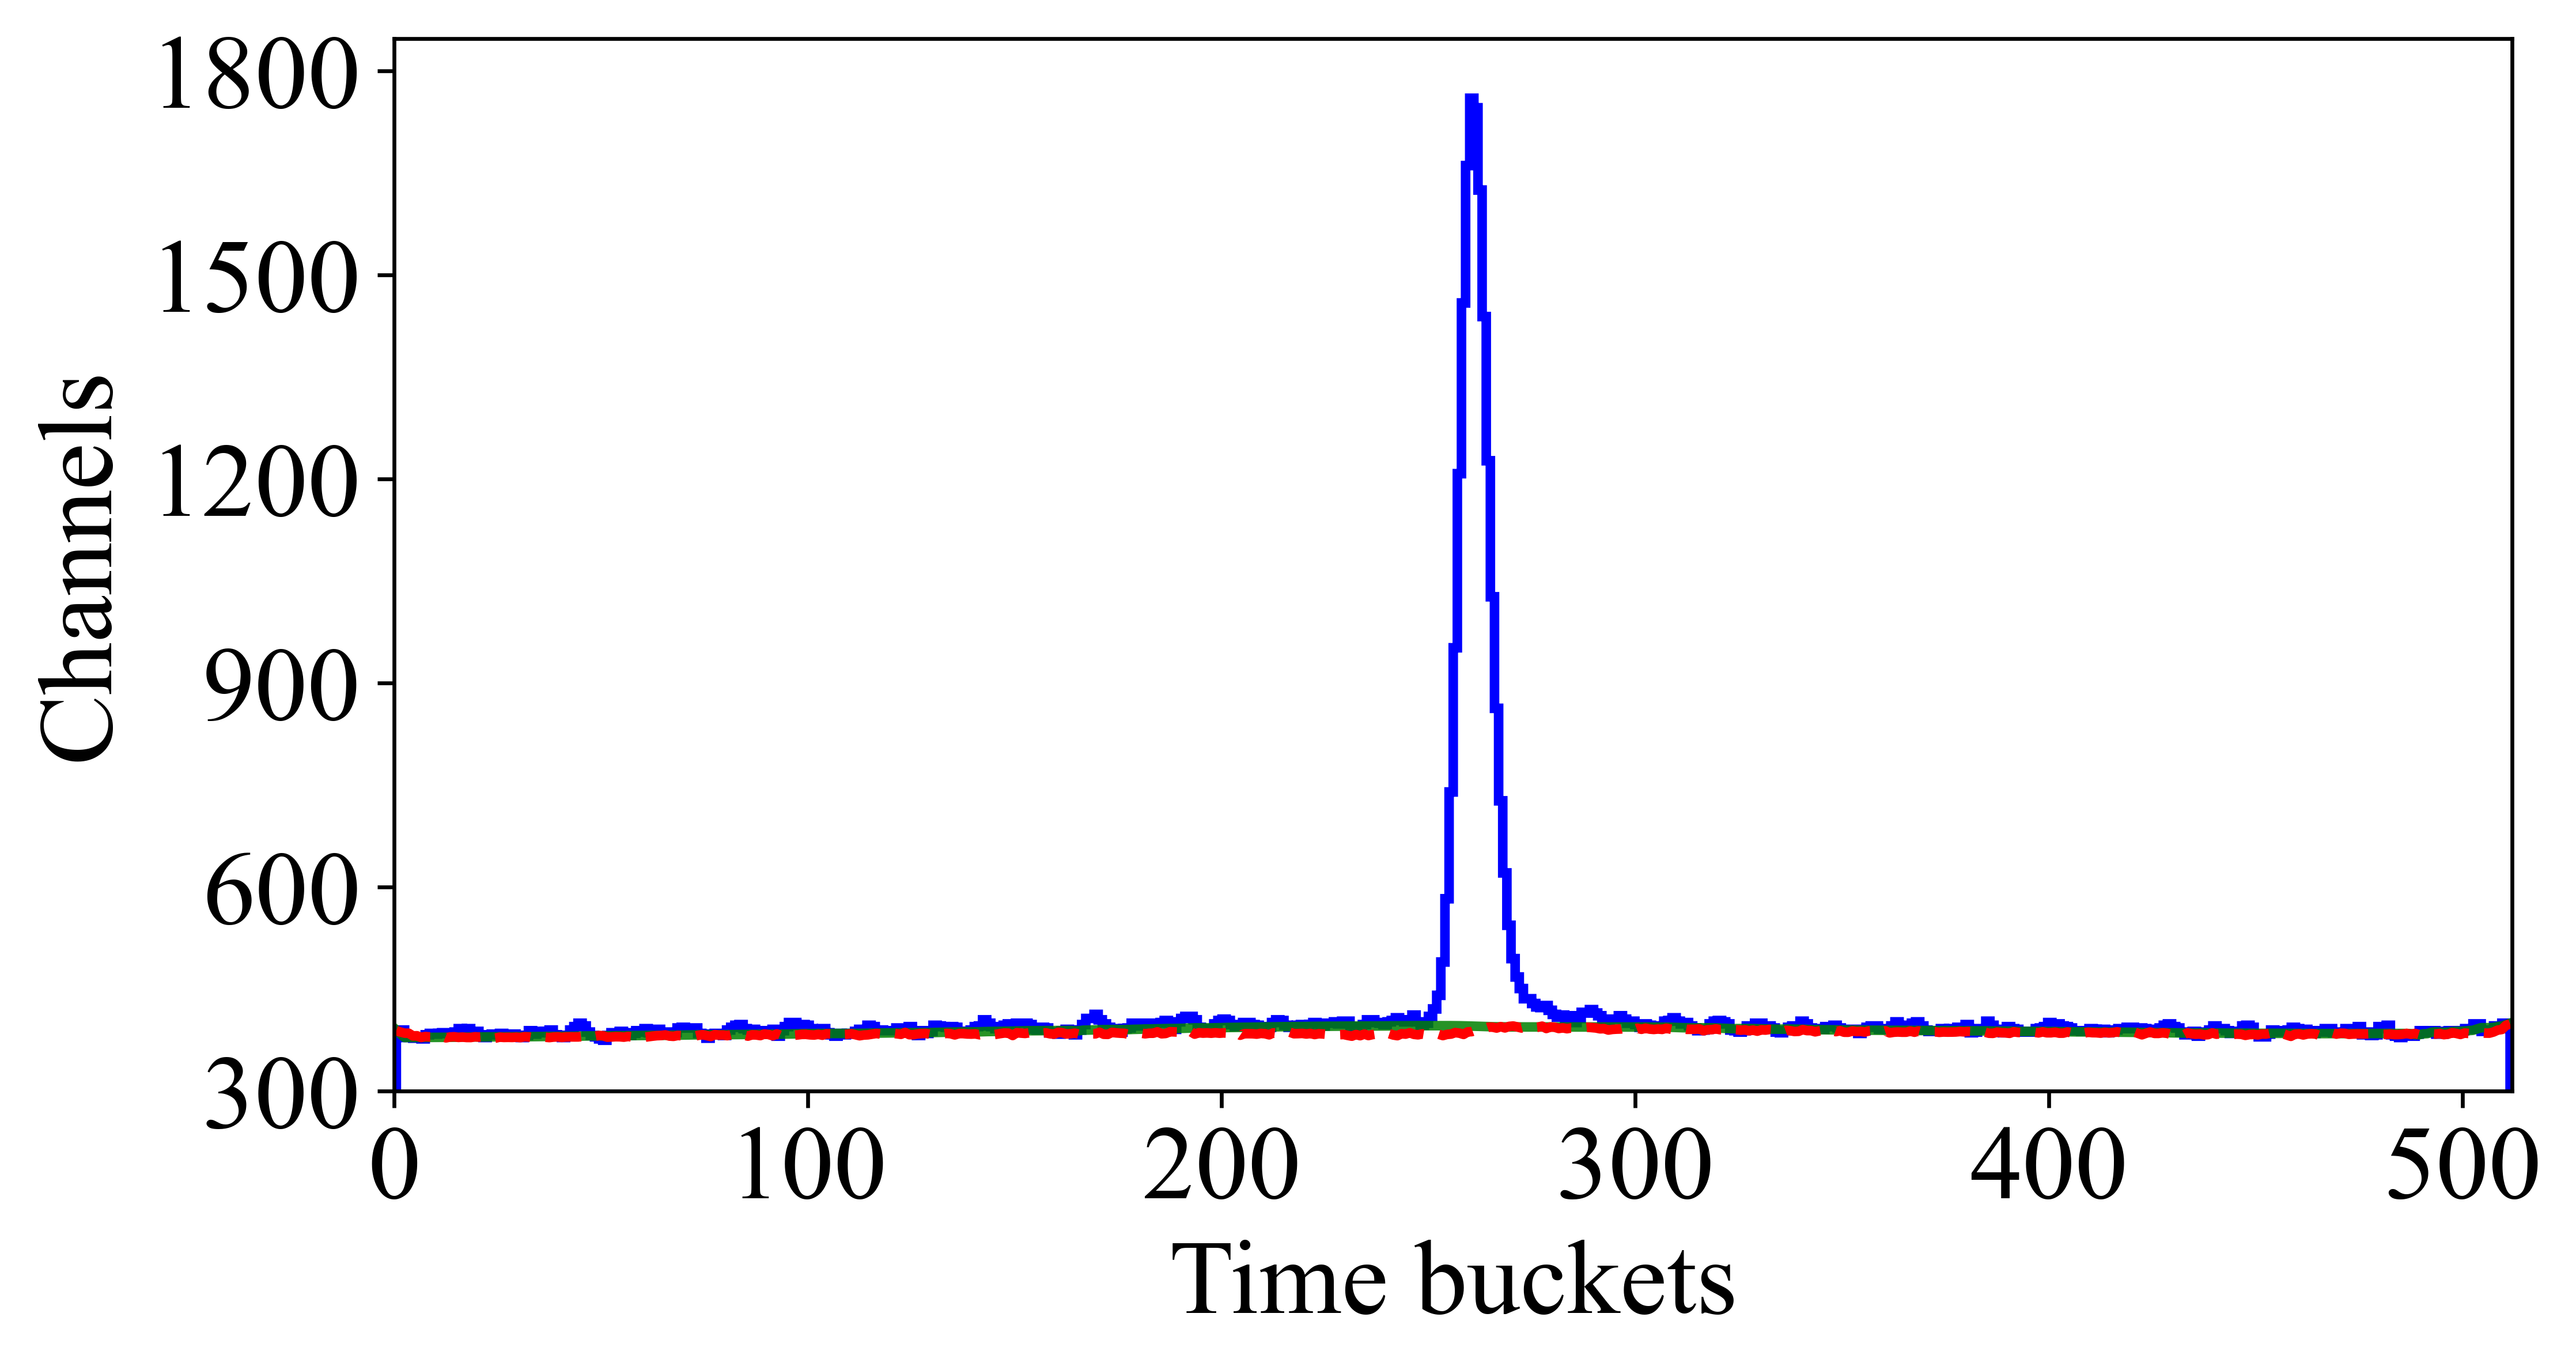
\includegraphics[scale=0.43]{figs/stb_2.png}
        \caption{}
        \label{subfig:stb_ex2}
    \end{subfigure}
    \begin{subfigure}[b]{0.47\textwidth}
        \centering
        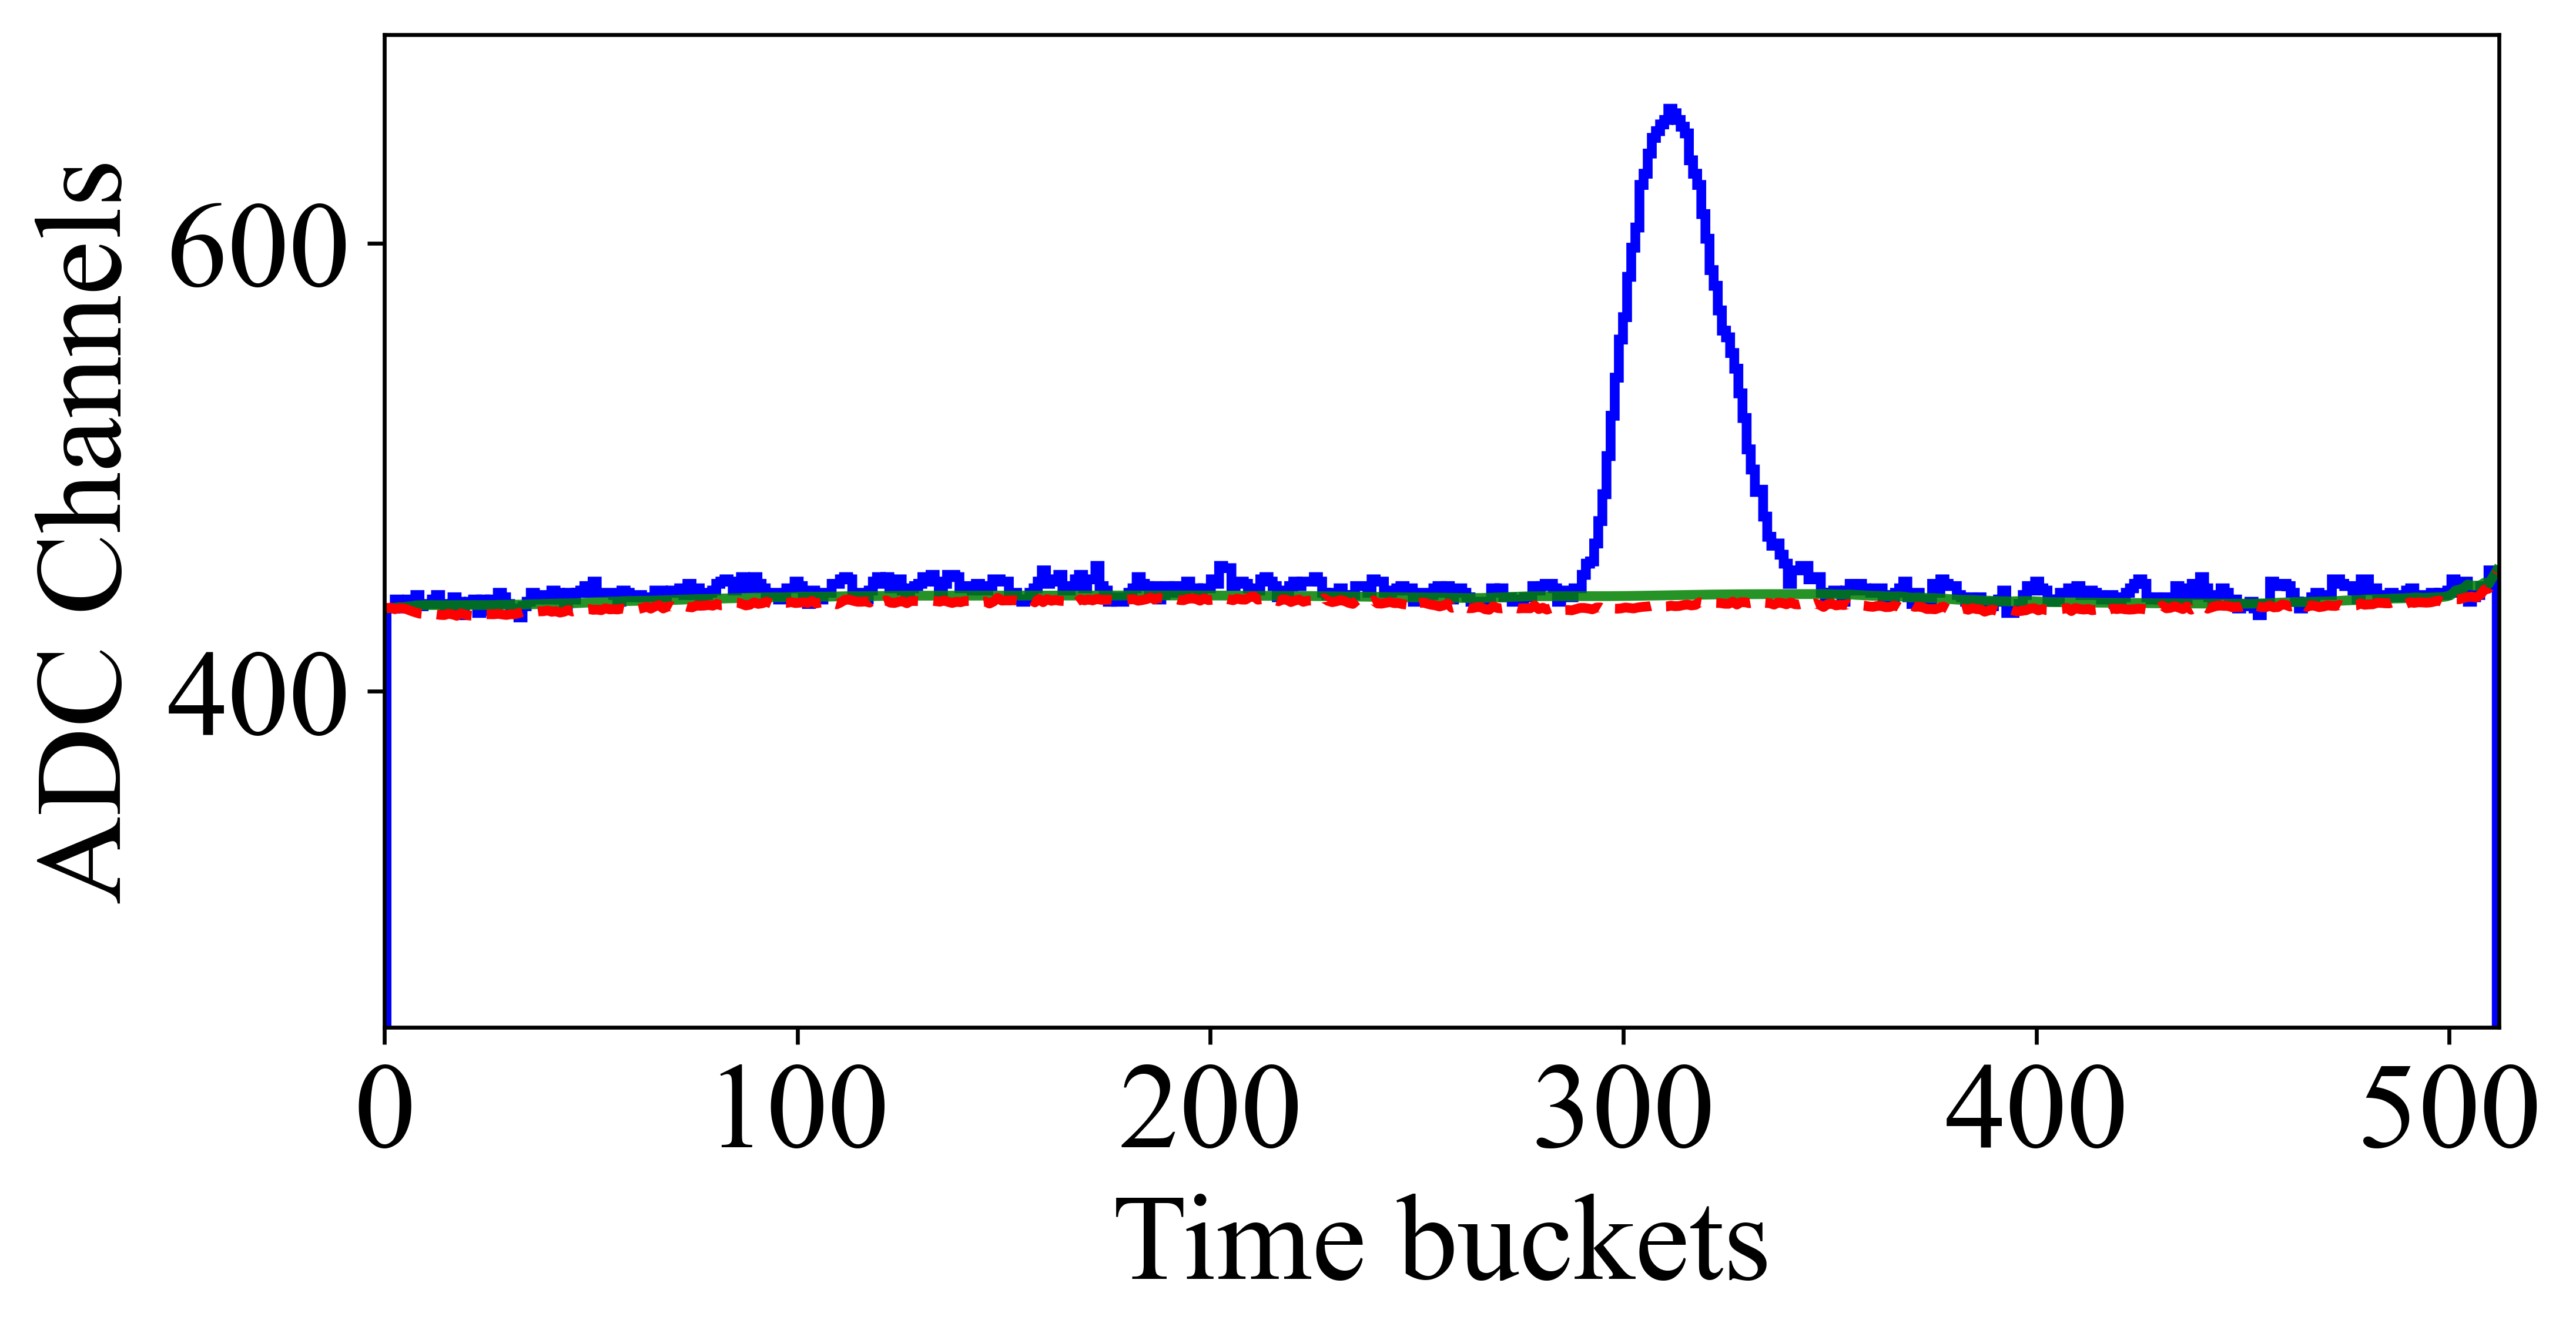
\includegraphics[scale=0.43]{figs/stb_3.png}
        \caption{}
        \label{subfig:stb_ex3}
    \end{subfigure}%
    \hfill
    \begin{subfigure}[b]{0.46\textwidth}
        \centering
        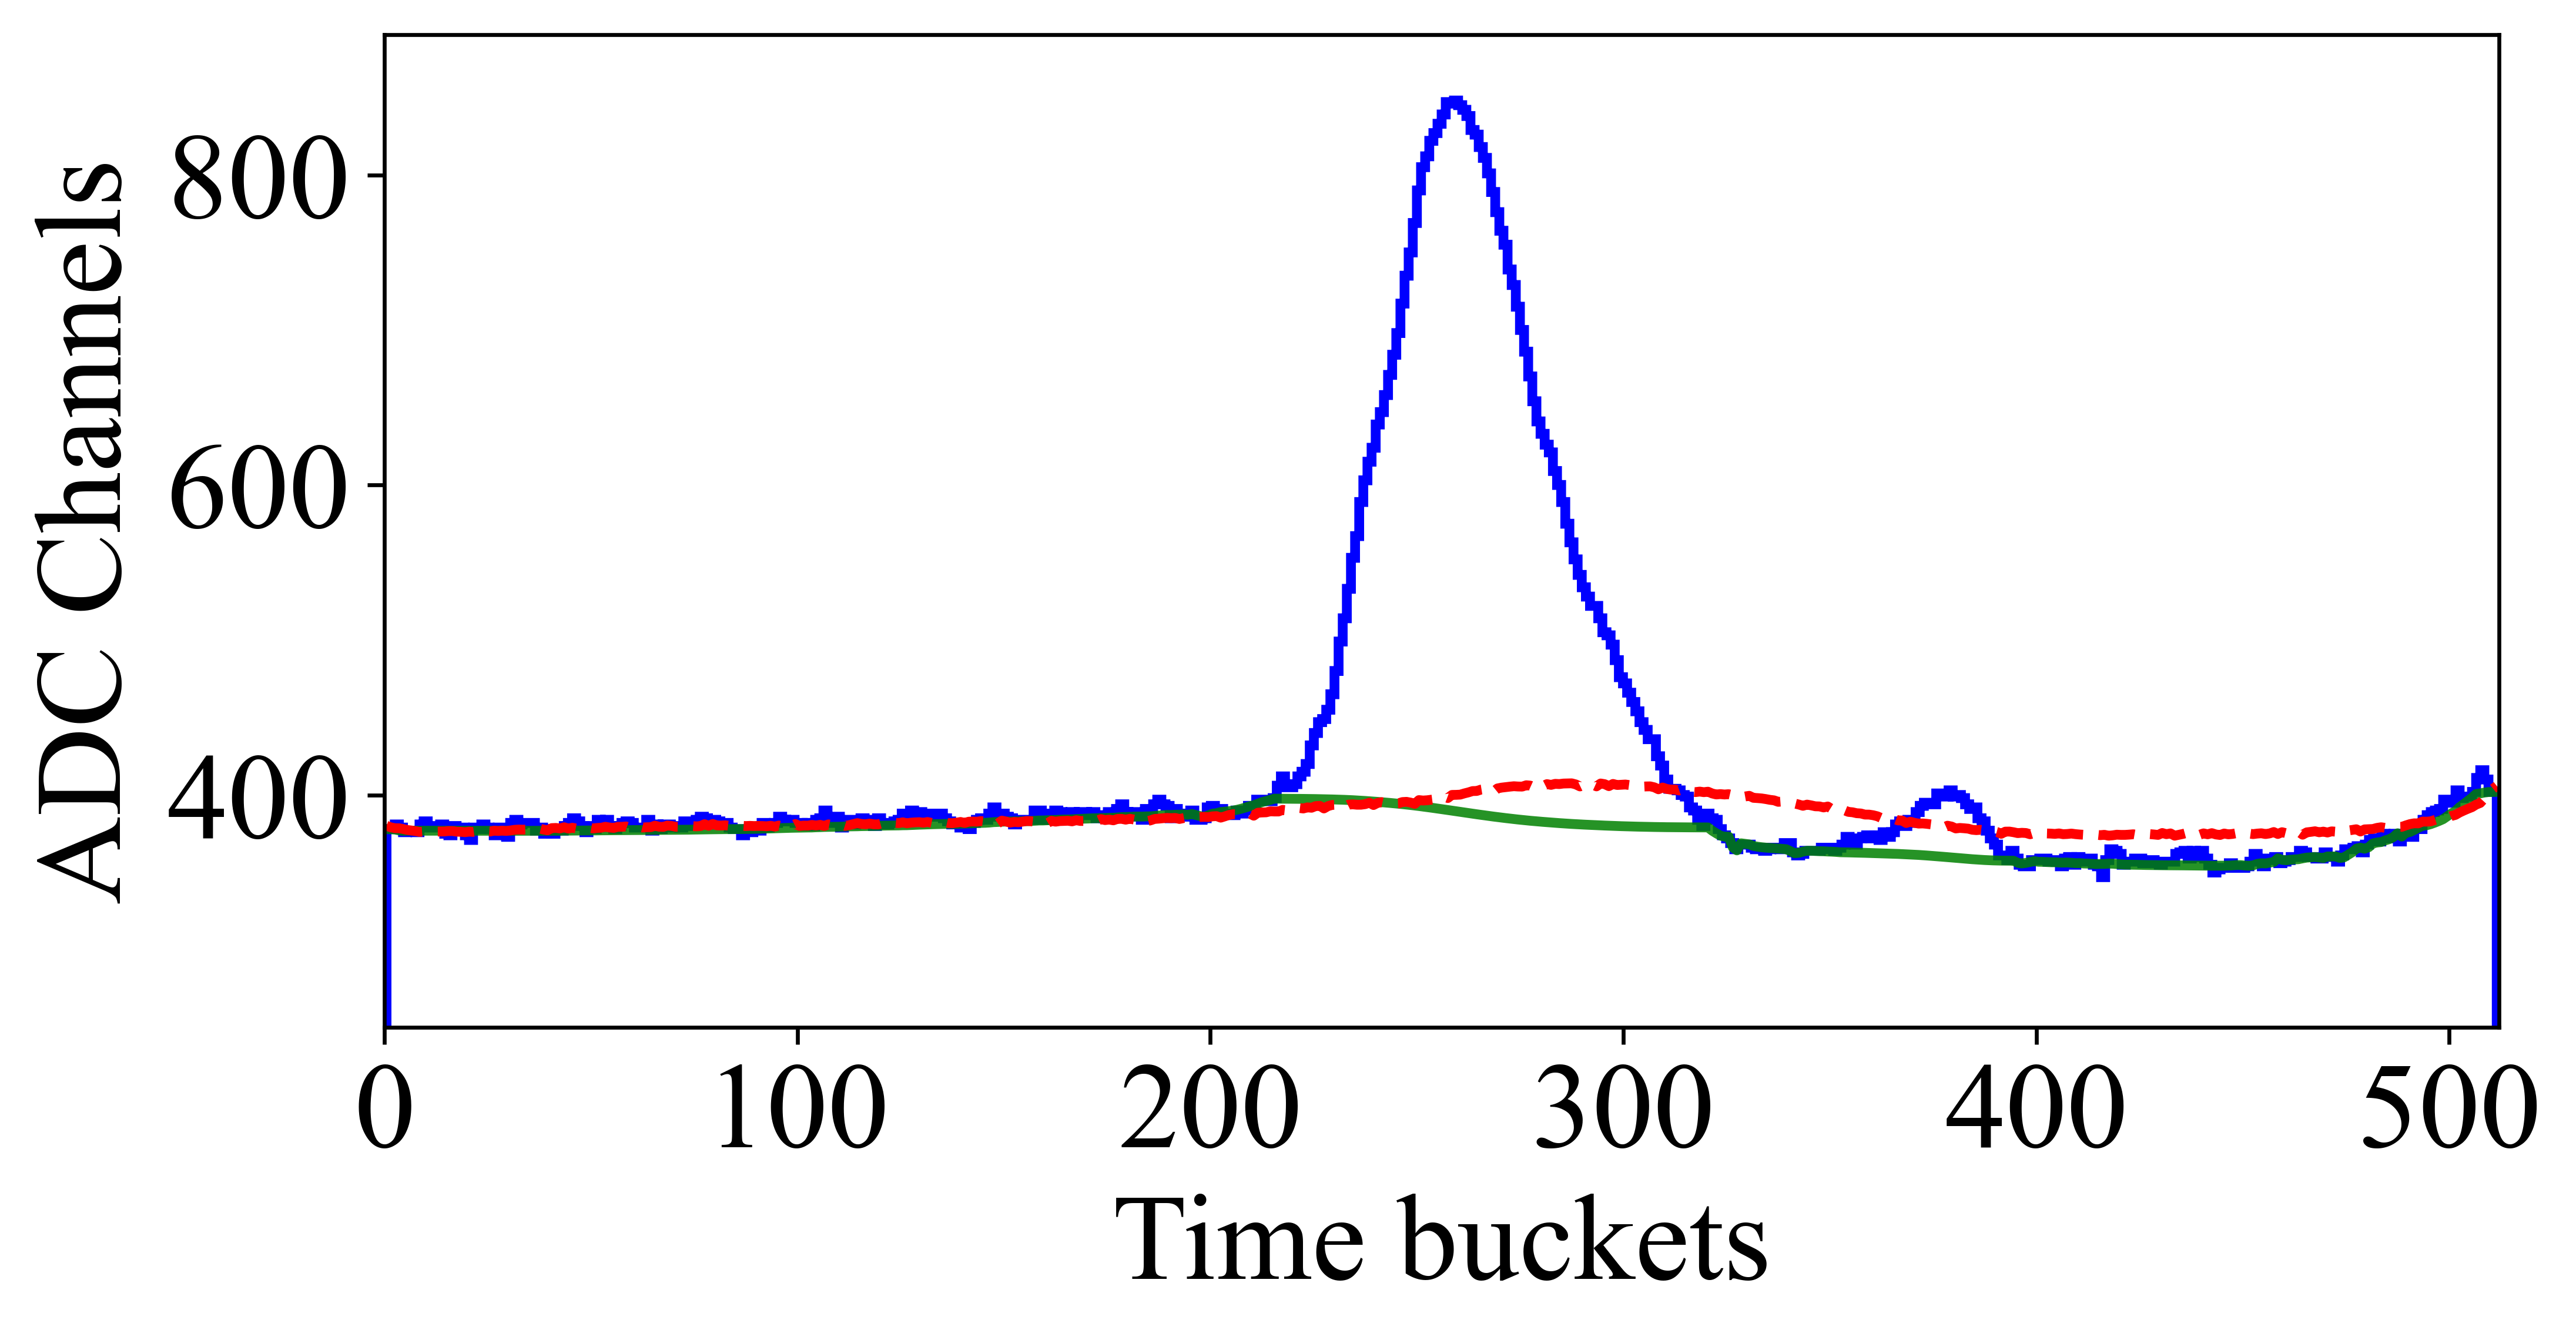
\includegraphics[scale=0.43]{figs/stb_4.png}
        \caption{}
        \label{subfig:stb_ex4}
    \end{subfigure}
\caption{Exemplos da rede neural dada pela figura \ref{fig:arq_source_to_bkg} em comparação com a saída do \textit{TSpectrum}.}
\label{fig:stb_examples}
\end{figure}

\par Nos exemplos mostrados nas figuras \ref{subfig:stb_ex1}, \ref{subfig:stb_ex2} e \ref{subfig:stb_ex1} os fundos dos sinais possuem grande flutuação e a rede neural se mostrou eficaz na previsão. No exemplo \ref{subfig:stb_ex4} a \textit{baseline} do sinal é muito complexa de se determinar, pois o sinal, aproximadamente do canal 300 a 500, varia em cerca de 50 unidades em \textit{y}. Apesar da rede neural determinar o fundo acima do fundo original, ao subtrair o espectro do fundo e colocar o valor mínimo em 0, o pulso presente entre os canais 200 e 300 é praticamente inalterado.

\par Com os resultados obtidos pela rede neural que calcula o sinal de fundo, o próximo passo foi criar a rede neural que faz a deconvolução do espectro sem a \textit{baseline}.

\subsection{Rede neural para a deconvolução}\label{subsec:pulso_ml_deconv}

% \par O próximo passo é construir uma rede neural que dê a posição dos picos. A tarefa a princípio não parece complicada. Pensando de forma simples, podemos fazer uma arquitetura curta e, como precisamos de uma saída de tamanho fixo, classificamos ponto a ponto como sendo não pico ou pico.

% \par O problema nessa abordagem é o desbalanço de classe evidente nos sinais. Caso tenhamos que classificar ponto a ponto em que, por exemplo, 0 representa um ponto que não é o centroide e 1 como um ponto que é um centroide, colocando na ultima camada a função de ativação \textit{sigmoid} (para sair valores entre 0 e 1), há muito mais valores 0 que 1. Se, por exemplo, temos um sinal que possui apenas um pico, teríamos que acertar o único valor 1 dentre 511 zeros. Caso a rede assuma que são 512 zeros, ainda assim a acurácia binária seria de mais de 99\%.

% \par Outro problema é que há um \textit{overlap} de gaussianas. Não é tão evidente a posição dos centroides se o espectro não está deconvoluído. É muito mais complicado, mesmo olhando, dizer a posição. Portanto o problema será quebrado em mais uma etapa: construir um rede que faça a deconvolução.

\par A mesma abordagem da rede neural anterior foi usada, que é fazer uma sequencia de convoluções e por fim uma camada \textit{fully connected} com função de ativação \textit{ReLU}, pois precisamos ter o valor mínimo do espectro em 0. Os filtros das convoluções precisam ter tamanho mínimo de duas vezes o sigma das gaussianas para atuarem sobre cada pulso do espectro. A entrada da rede é o sinal com o fundo subtraído e com mínimo em 0. A saída é o sinal após deconvolução dada pelo algoritmo \textit{gold deconvolution} na biblioteca \textit{TSpectrum} do ROOT, já mostrado na subseção \ref{subsec:pulses_deconv}. A figura \ref{fig:source_to_deconv} mostra a arquitetura da rede de deconvolução.

\par A rede é a sequência de duas convoluções com 32 filtros, \textit{valid padding} e \textit{kernels} de tamanho 19 e 17, respectivamente, seguida de uma camada \textit{Max pooling} com \textit{pool size} igual à 16. No final há o \textit{flat} na camada para seguir com uma camada \textit{fully connected} com função de ativação \textit{ReLU}. O \textit{valid padding} se mostrou mais eficiente para a convergência da rede. Toda a rede foi construída usando o TensorFlow 2, possuindo 508.000 parâmetros treináveis \cite{FORTINO2022166497}.

\par Assim como na rede anterior, foram usados 160.000 sinais para treino e 40.000 para validação. O \textit{loss} foi escolhido como sendo o erro quadrático médio, o otimizador foi o \textit{ADAM}, com \textit{learning rate} de 0.0005 porém com o parâmetro \textit{clipnorm} igual a 0.45. A métrica para avaliação foi o erro médio absoluto. Foram 75 \textit{epochs} e o \textit{batch-size} foi 8. Os resultados do treino estão na figura \ref{fig:source_wo_bkg_to_deconv_results}.

\par Alterar a norma do gradiente (usar o parâmetro \textit{clipnorm} = 0.45) significa que, caso a norma do vetor do gradiente exceda 0.45, então o valor da norma é reajustado para o limiar (\textit{threshold}) escolhido (0.45) \cite{FORTINO2022166497}. Isso faz com que não ocorra problemas comuns como o gradiente sumir \cite{VGP, ADAMAX}, um dos problemas que teve que ser resolvido nessa rede.

\par O treino foi realizado no Google Colaboratory \cite{google_colab} usando a GPU NVIDIA Tesla P100 e demorou cerca de 54 minutos. Os resultados do treino estão na figura \ref{fig:source_to_bkg_results}, onde eles indicam que, visualmente, a rede neural consegue distinguir muito bem diferentes centroides presentes no pulso. Empiricamente, a rede é capaz de executar 200.000 sinais em 5.4 segundos (ou 37.000 sinais por segundo).

\begin{figure}[H]
    \centering
    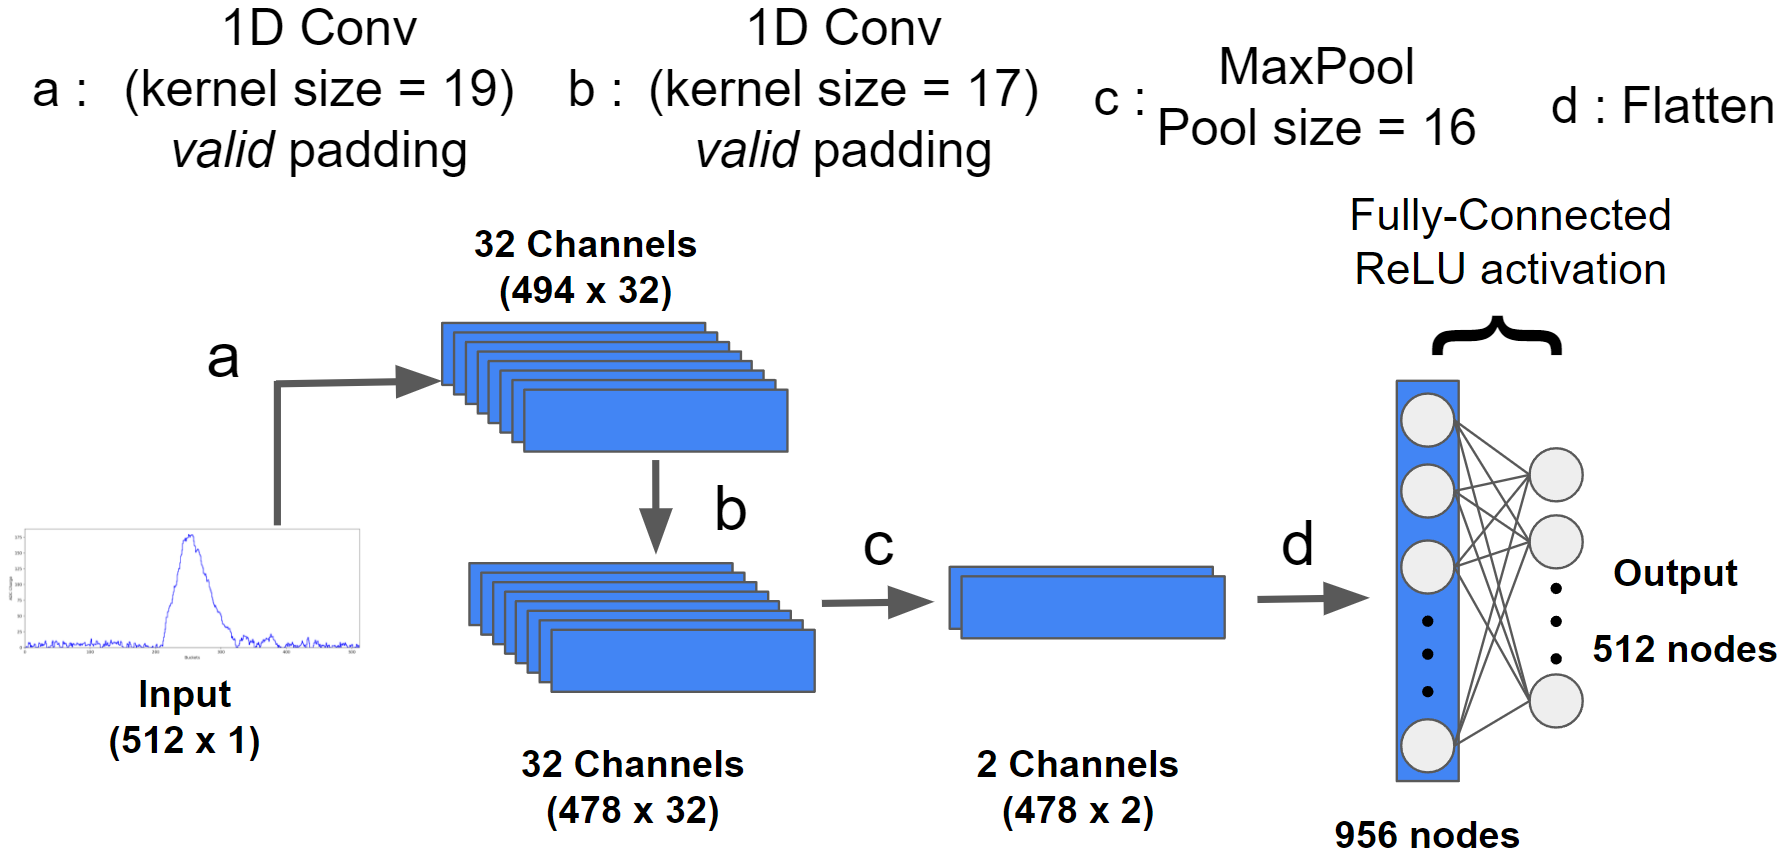
\includegraphics[scale = 0.28]{figs/source_wobkg_to_deconv.png}
    \caption{Arquitetura da rede neural que faz a inferência da deconvolução do espectro. O vetor de entrada deve ter dimensionalidade 512 x 1. Todas as partes com convolução não possuem o parâmetro \textit{bias}.}
    \label{fig:source_to_deconv}
\end{figure}

\begin{figure}[H]
\centering
    \begin{subfigure}[t]{0.49\textwidth}
        \centering
        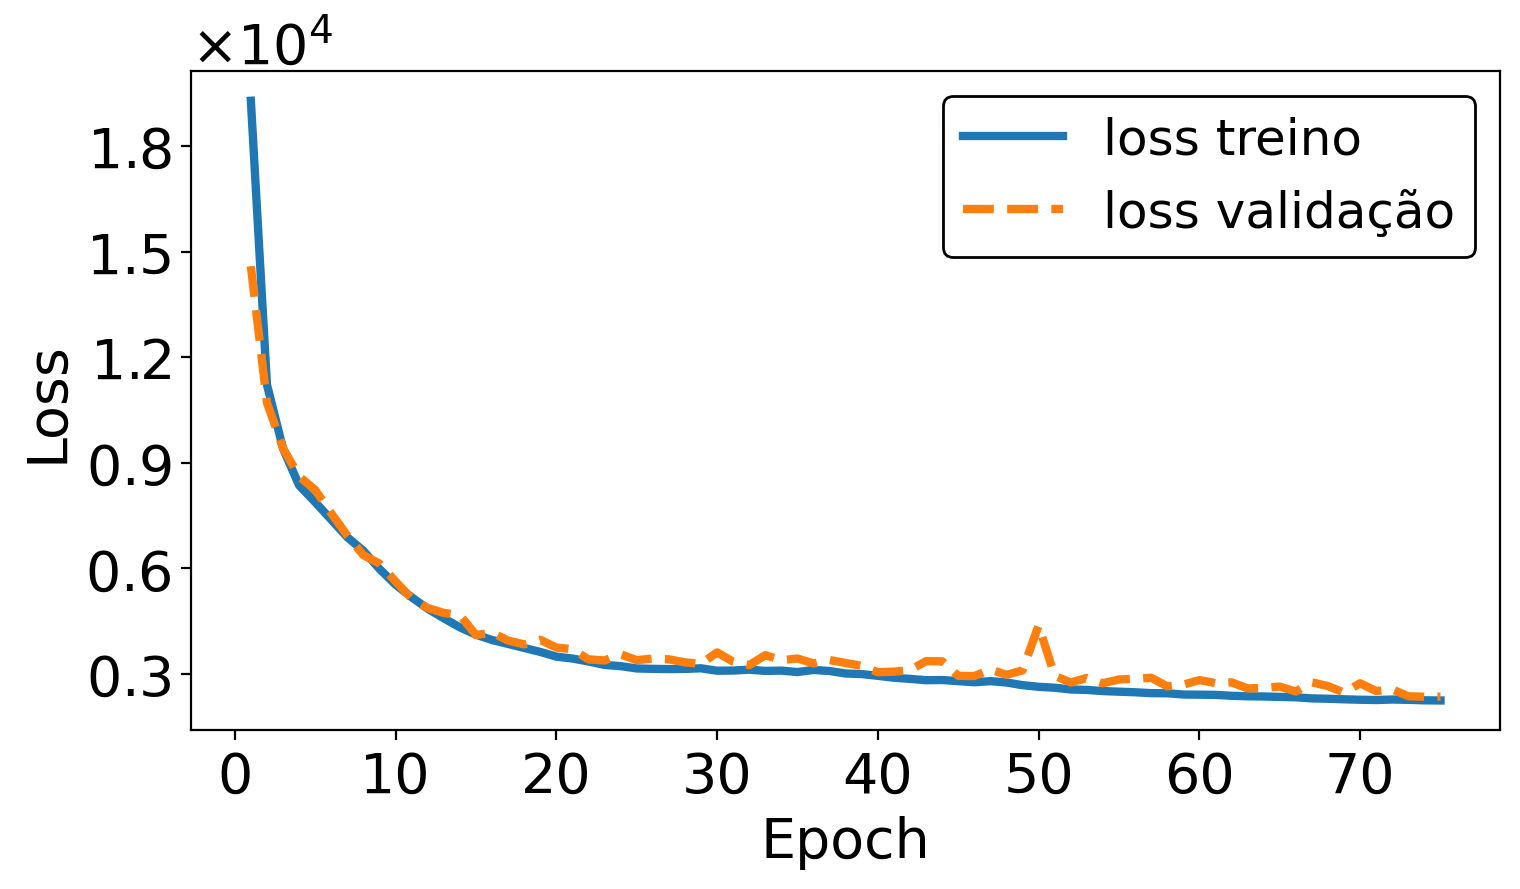
\includegraphics[scale=0.42]{figs/source_wo_bkg_to_deconv_loss.png}
        \caption{\textit{Loss} dos dados de treino (linha contínua) e dos dados de validação (linha tracejada) em função da \textit{epoch} no treino da rede dada pela figura \ref{fig:source_to_deconv}.}
        \label{subfig:source_wo_bkg_to_deconv_loss}
    \end{subfigure}%
    \hfill
    \begin{subfigure}[t]{0.465\textwidth}
        \centering
        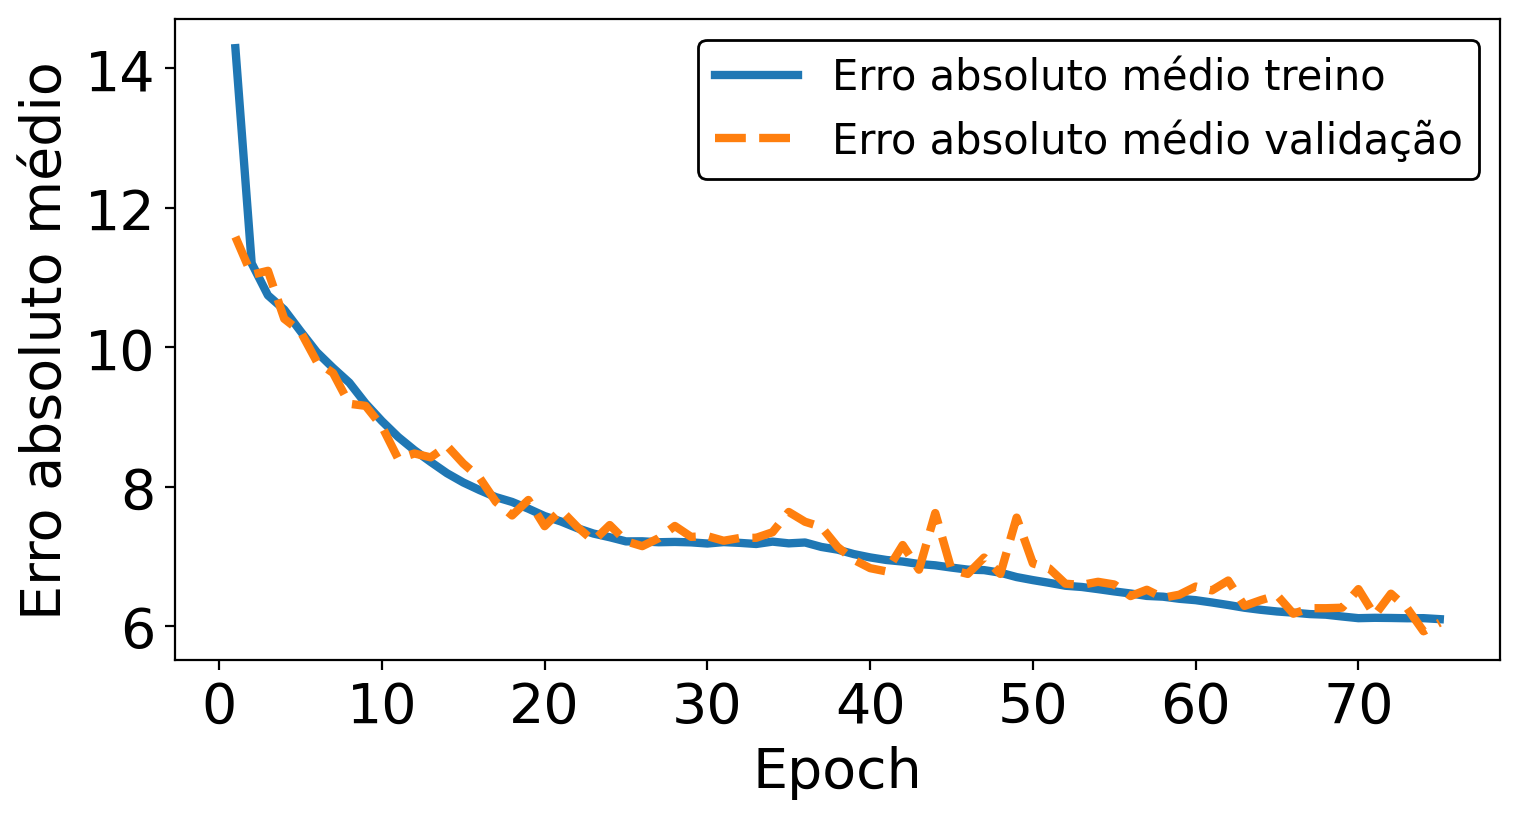
\includegraphics[scale=0.42]{figs/source_wo_bkg_to_deconv_metric.png}
        \caption{Erro absoluto médio dos dados de treino (linha contínua) e dos dados de validação (linha tracejada) em função da \textit{epoch} no treino da rede dada pela figura \ref{fig:source_to_deconv}.}
        \label{subfig:source_wo_bkg_to_deconv_metric}
    \end{subfigure}
\caption{Resultados do treino da rede neural dada pela figura \ref{fig:arq_source_to_bkg}.}
\label{fig:source_wo_bkg_to_deconv_results}
\end{figure}

% \par A mudança em relação à rede que faz a inferência do sinal de fundo é que o \textit{padding} das camadas agora é \textit{valid}. Agora não estamos verificando pontos onde seriam necessários adicionar zeros além do vetor de entrada, como explicado na seção \ref{sec:ml}. O \textit{padding} \textit{valid} se mostrou mais eficiente com relação à separação das gaussianas, dando melhor resolução para buscar os centroides. Além disso, ao colocar o \textit{pool size} de apenas 16, para poder dar um \textit{flat} na camada seguinte, fez com que a resolução de separação das gaussianas fosse inclusive melhor que a do algoritmo analítico. A figura \ref{fig:std_examples} mostra um exemplo da saída da rede.

\begin{figure}[H]
\centering
    \begin{subfigure}[b]{0.49\textwidth}
        \centering
        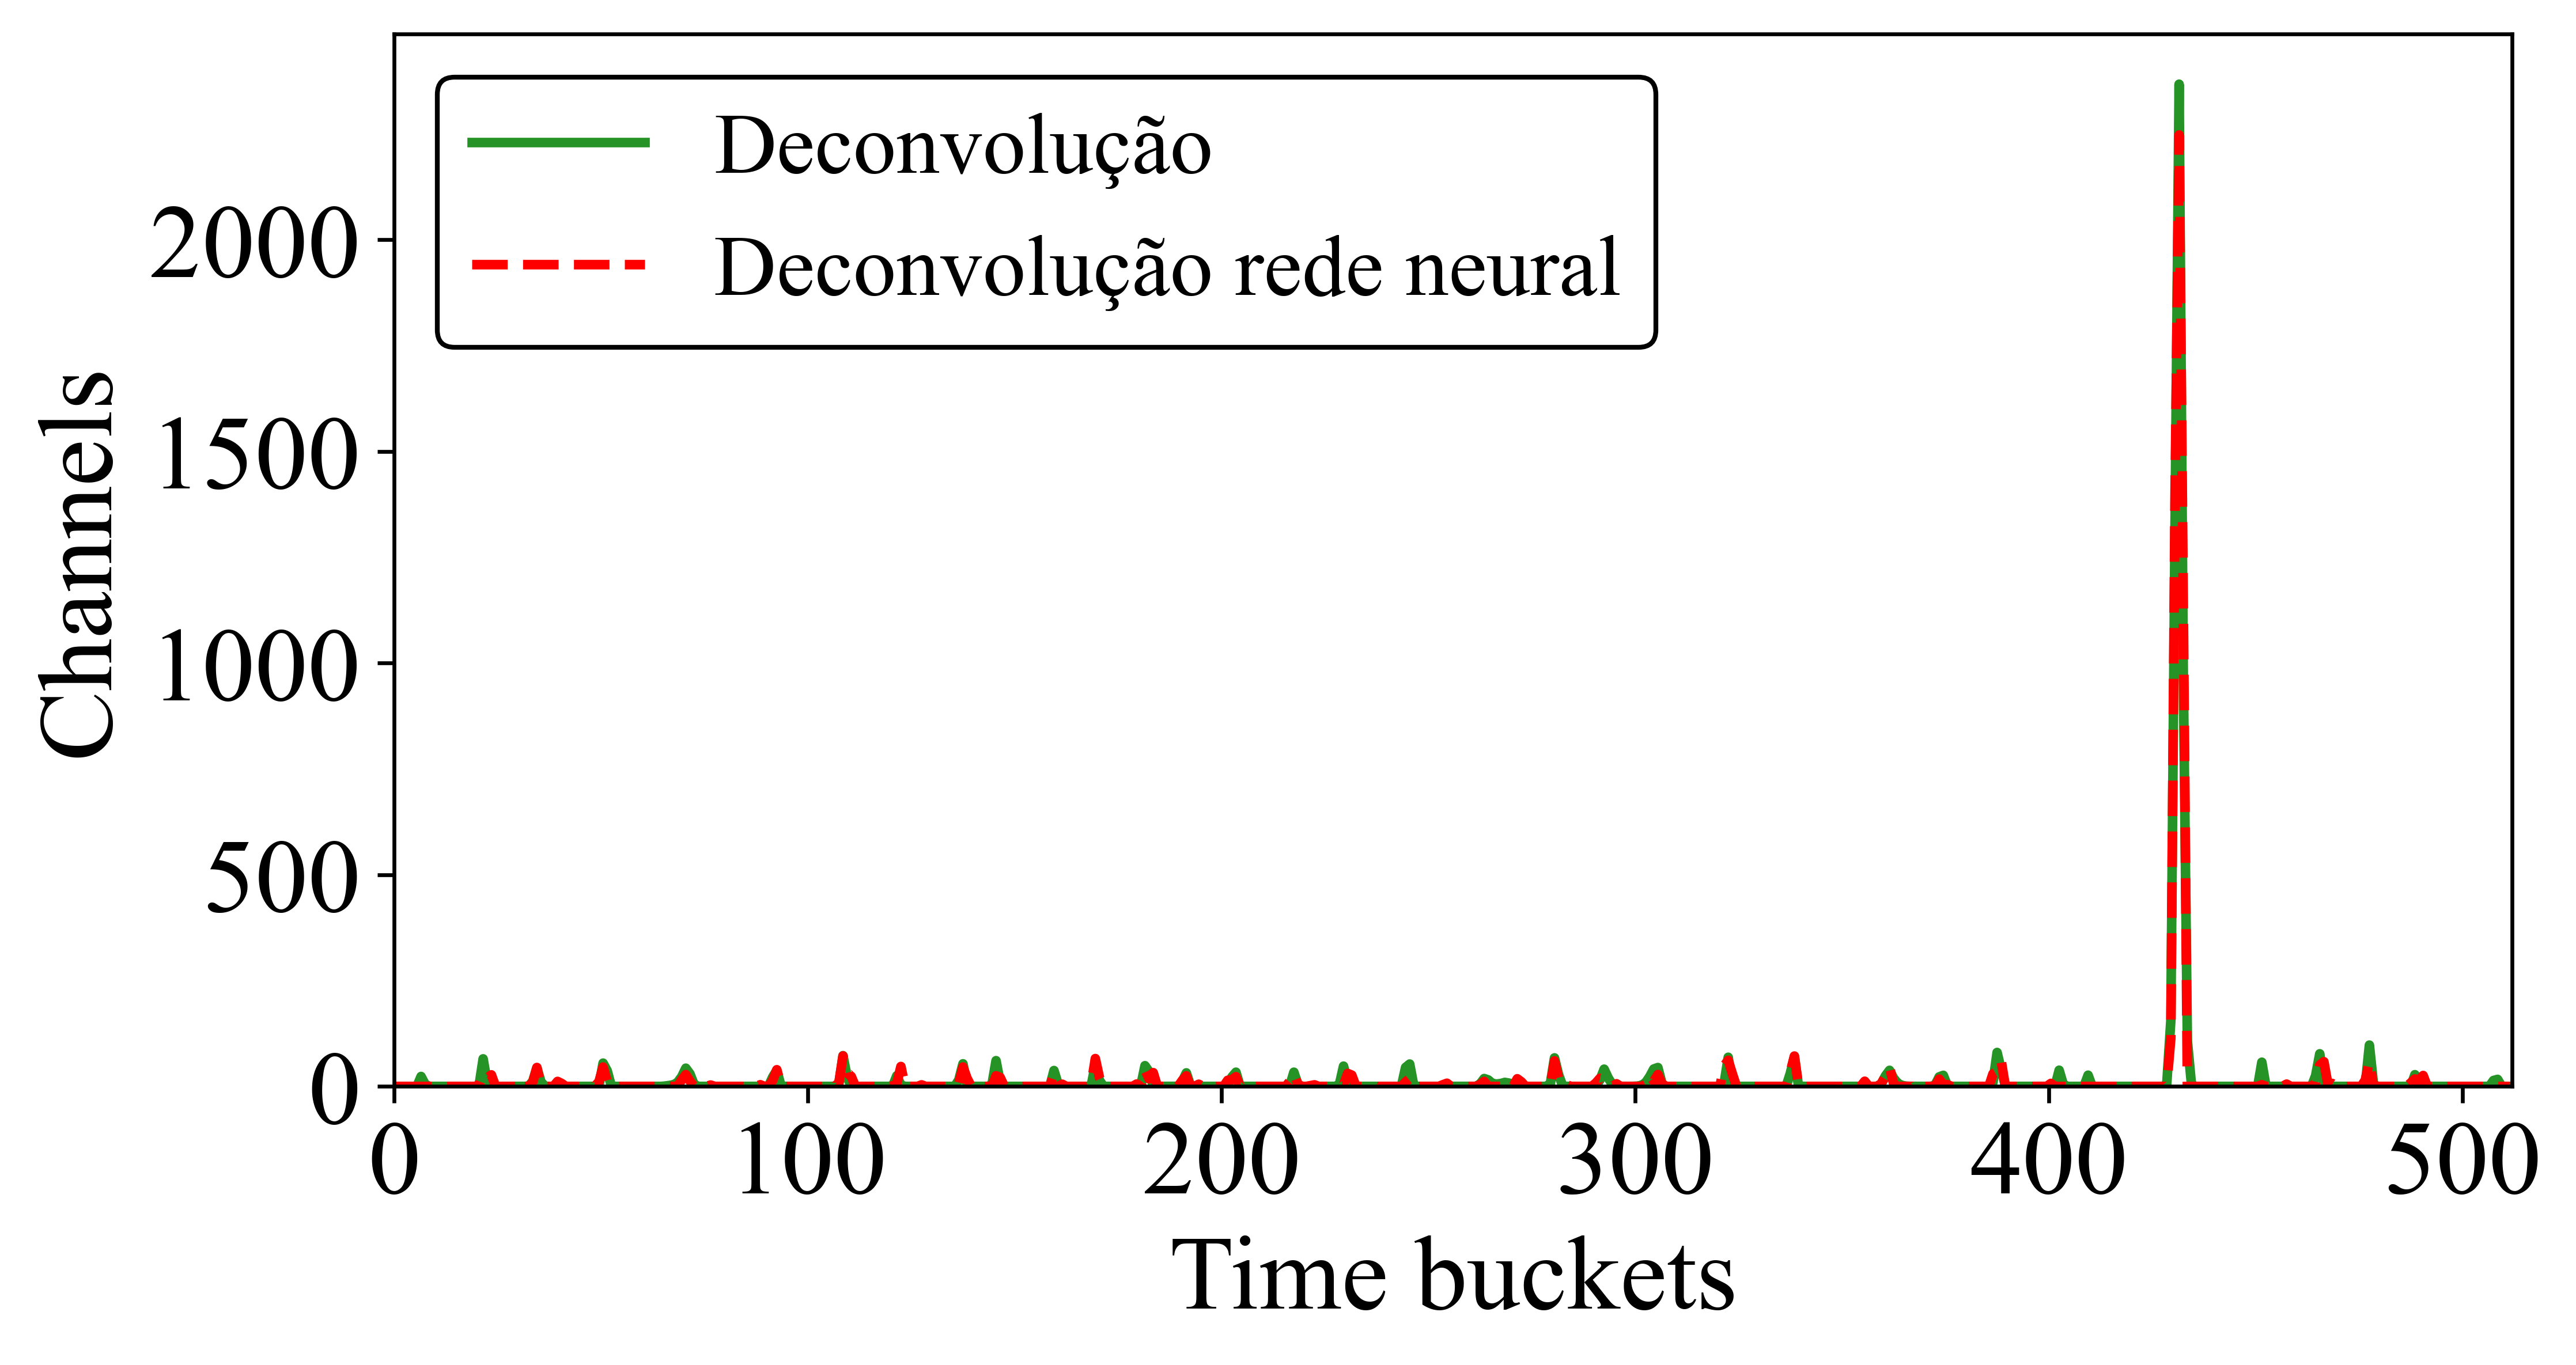
\includegraphics[scale=0.425]{figs/swbtd_1.png}
        \caption{}
        \label{subfig:std_ex1}
    \end{subfigure}%
    \hfill
    \begin{subfigure}[b]{0.465\textwidth}
        \centering
        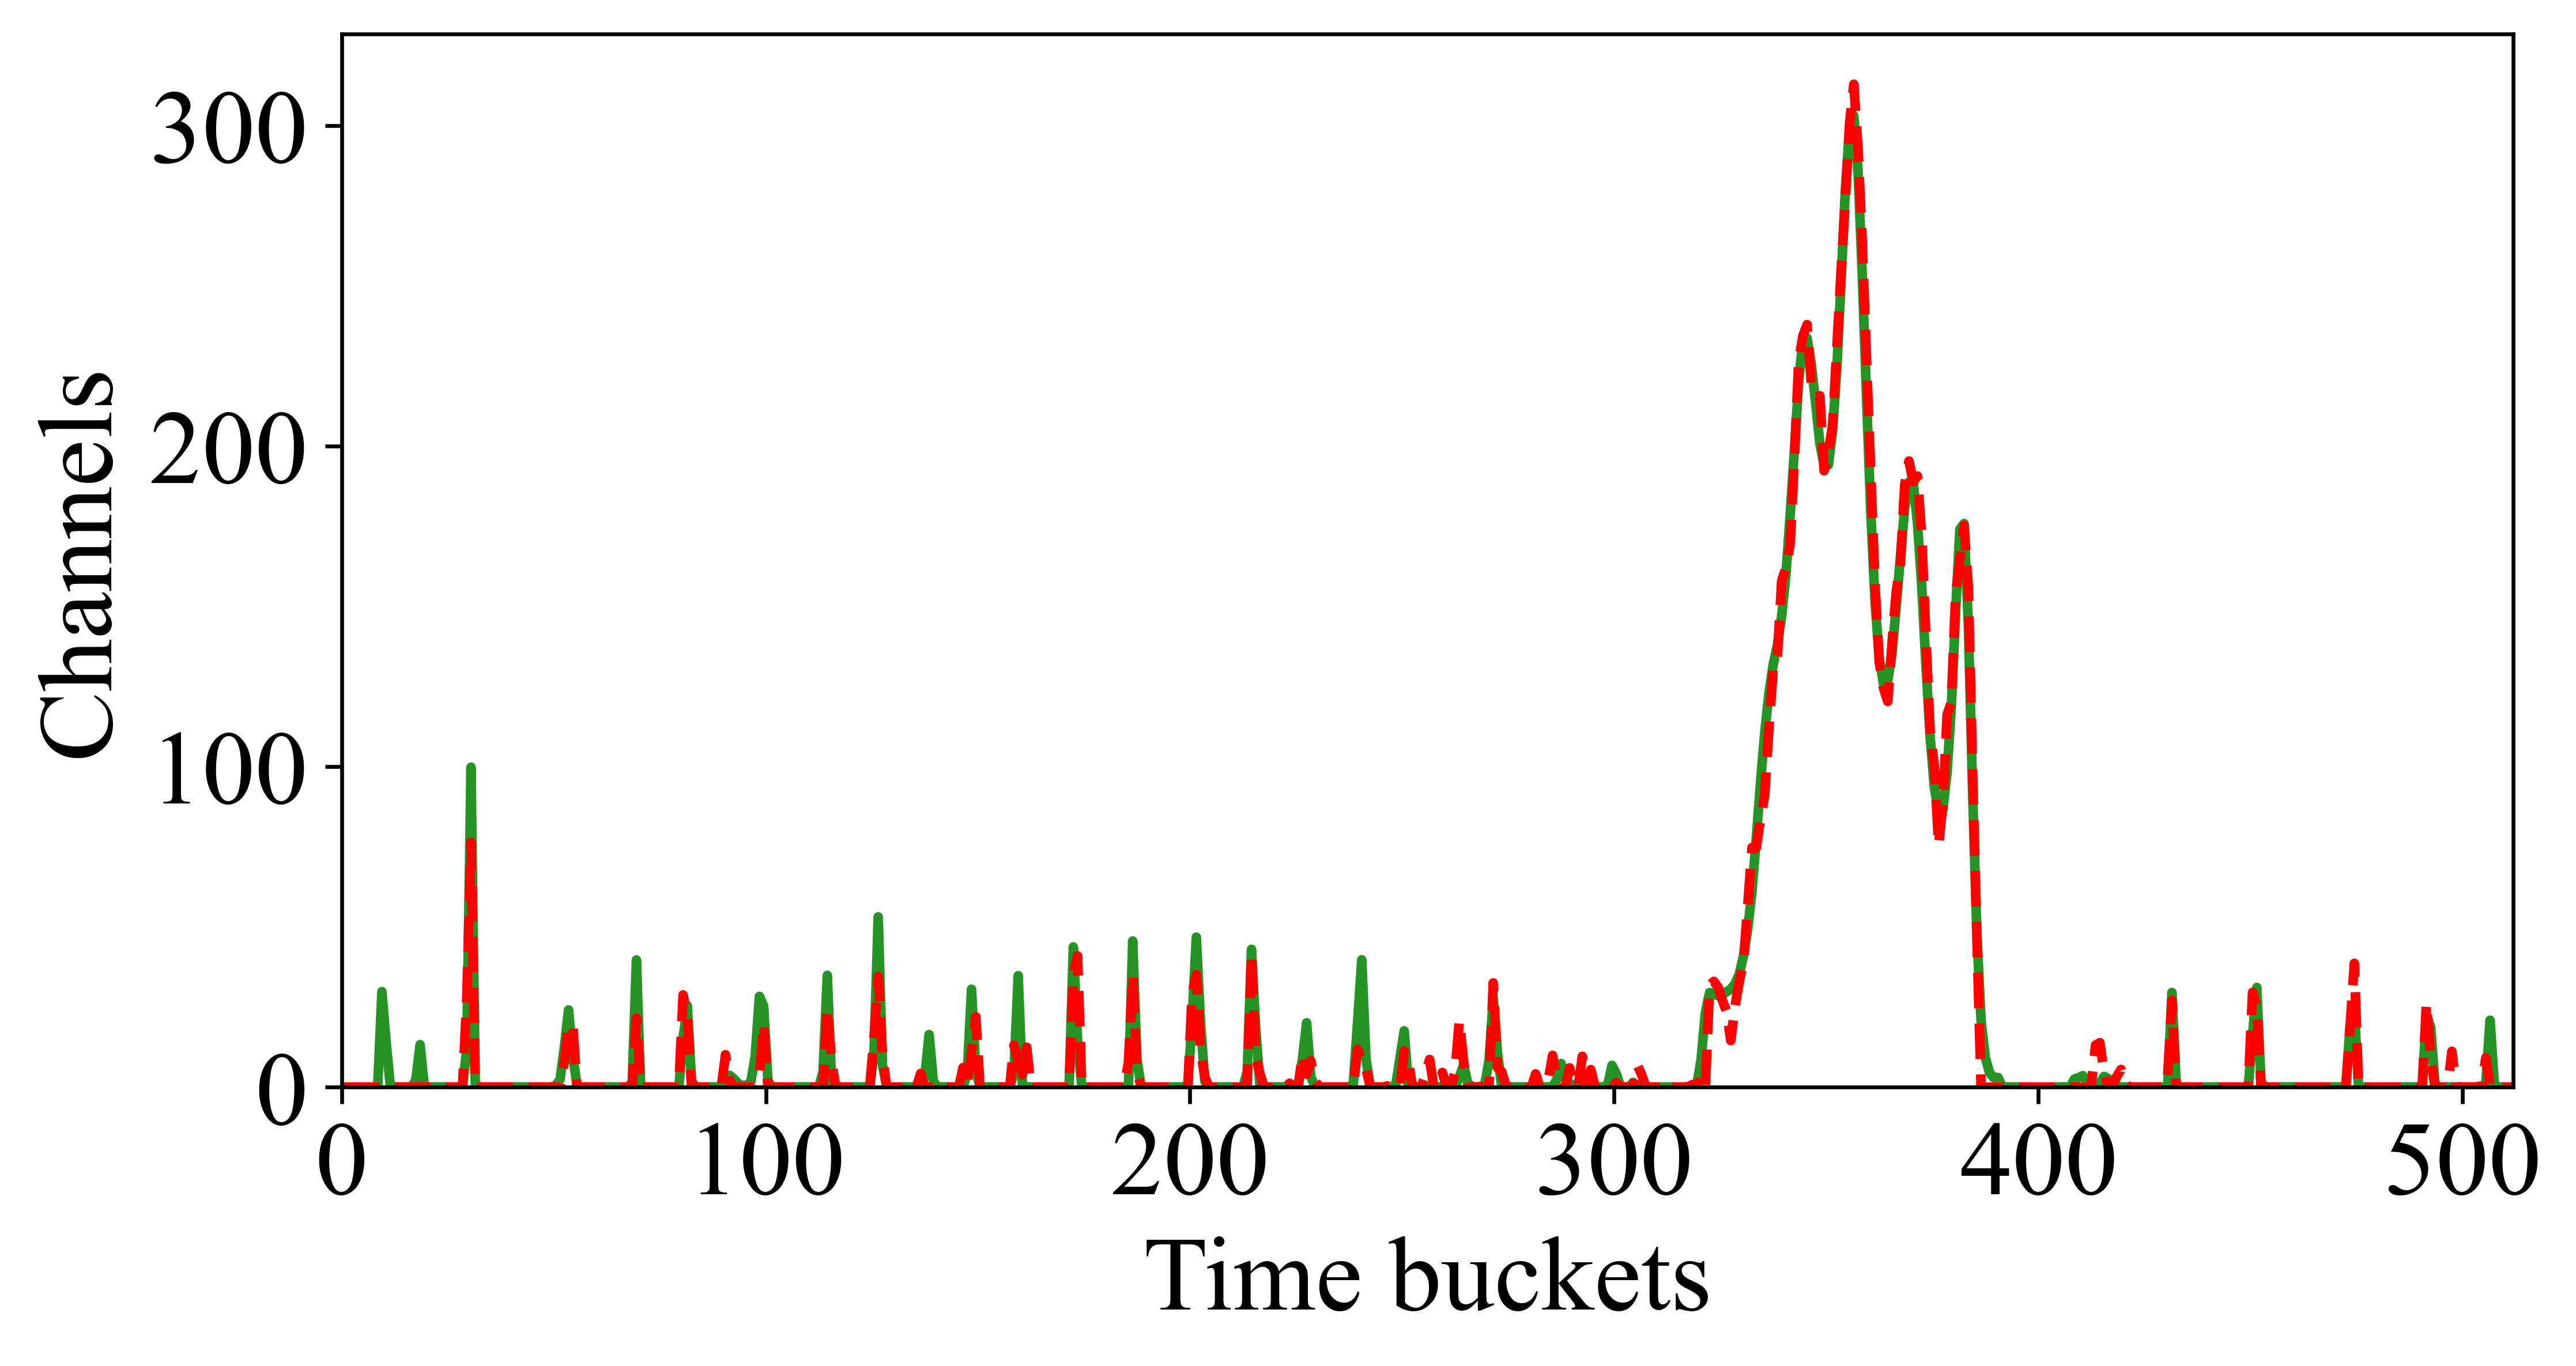
\includegraphics[scale=0.425]{figs/swbtd_2.png}
        \caption{}
        \label{subfig:std_ex2}
    \end{subfigure}
    \begin{subfigure}[b]{0.49\textwidth}
        \centering
        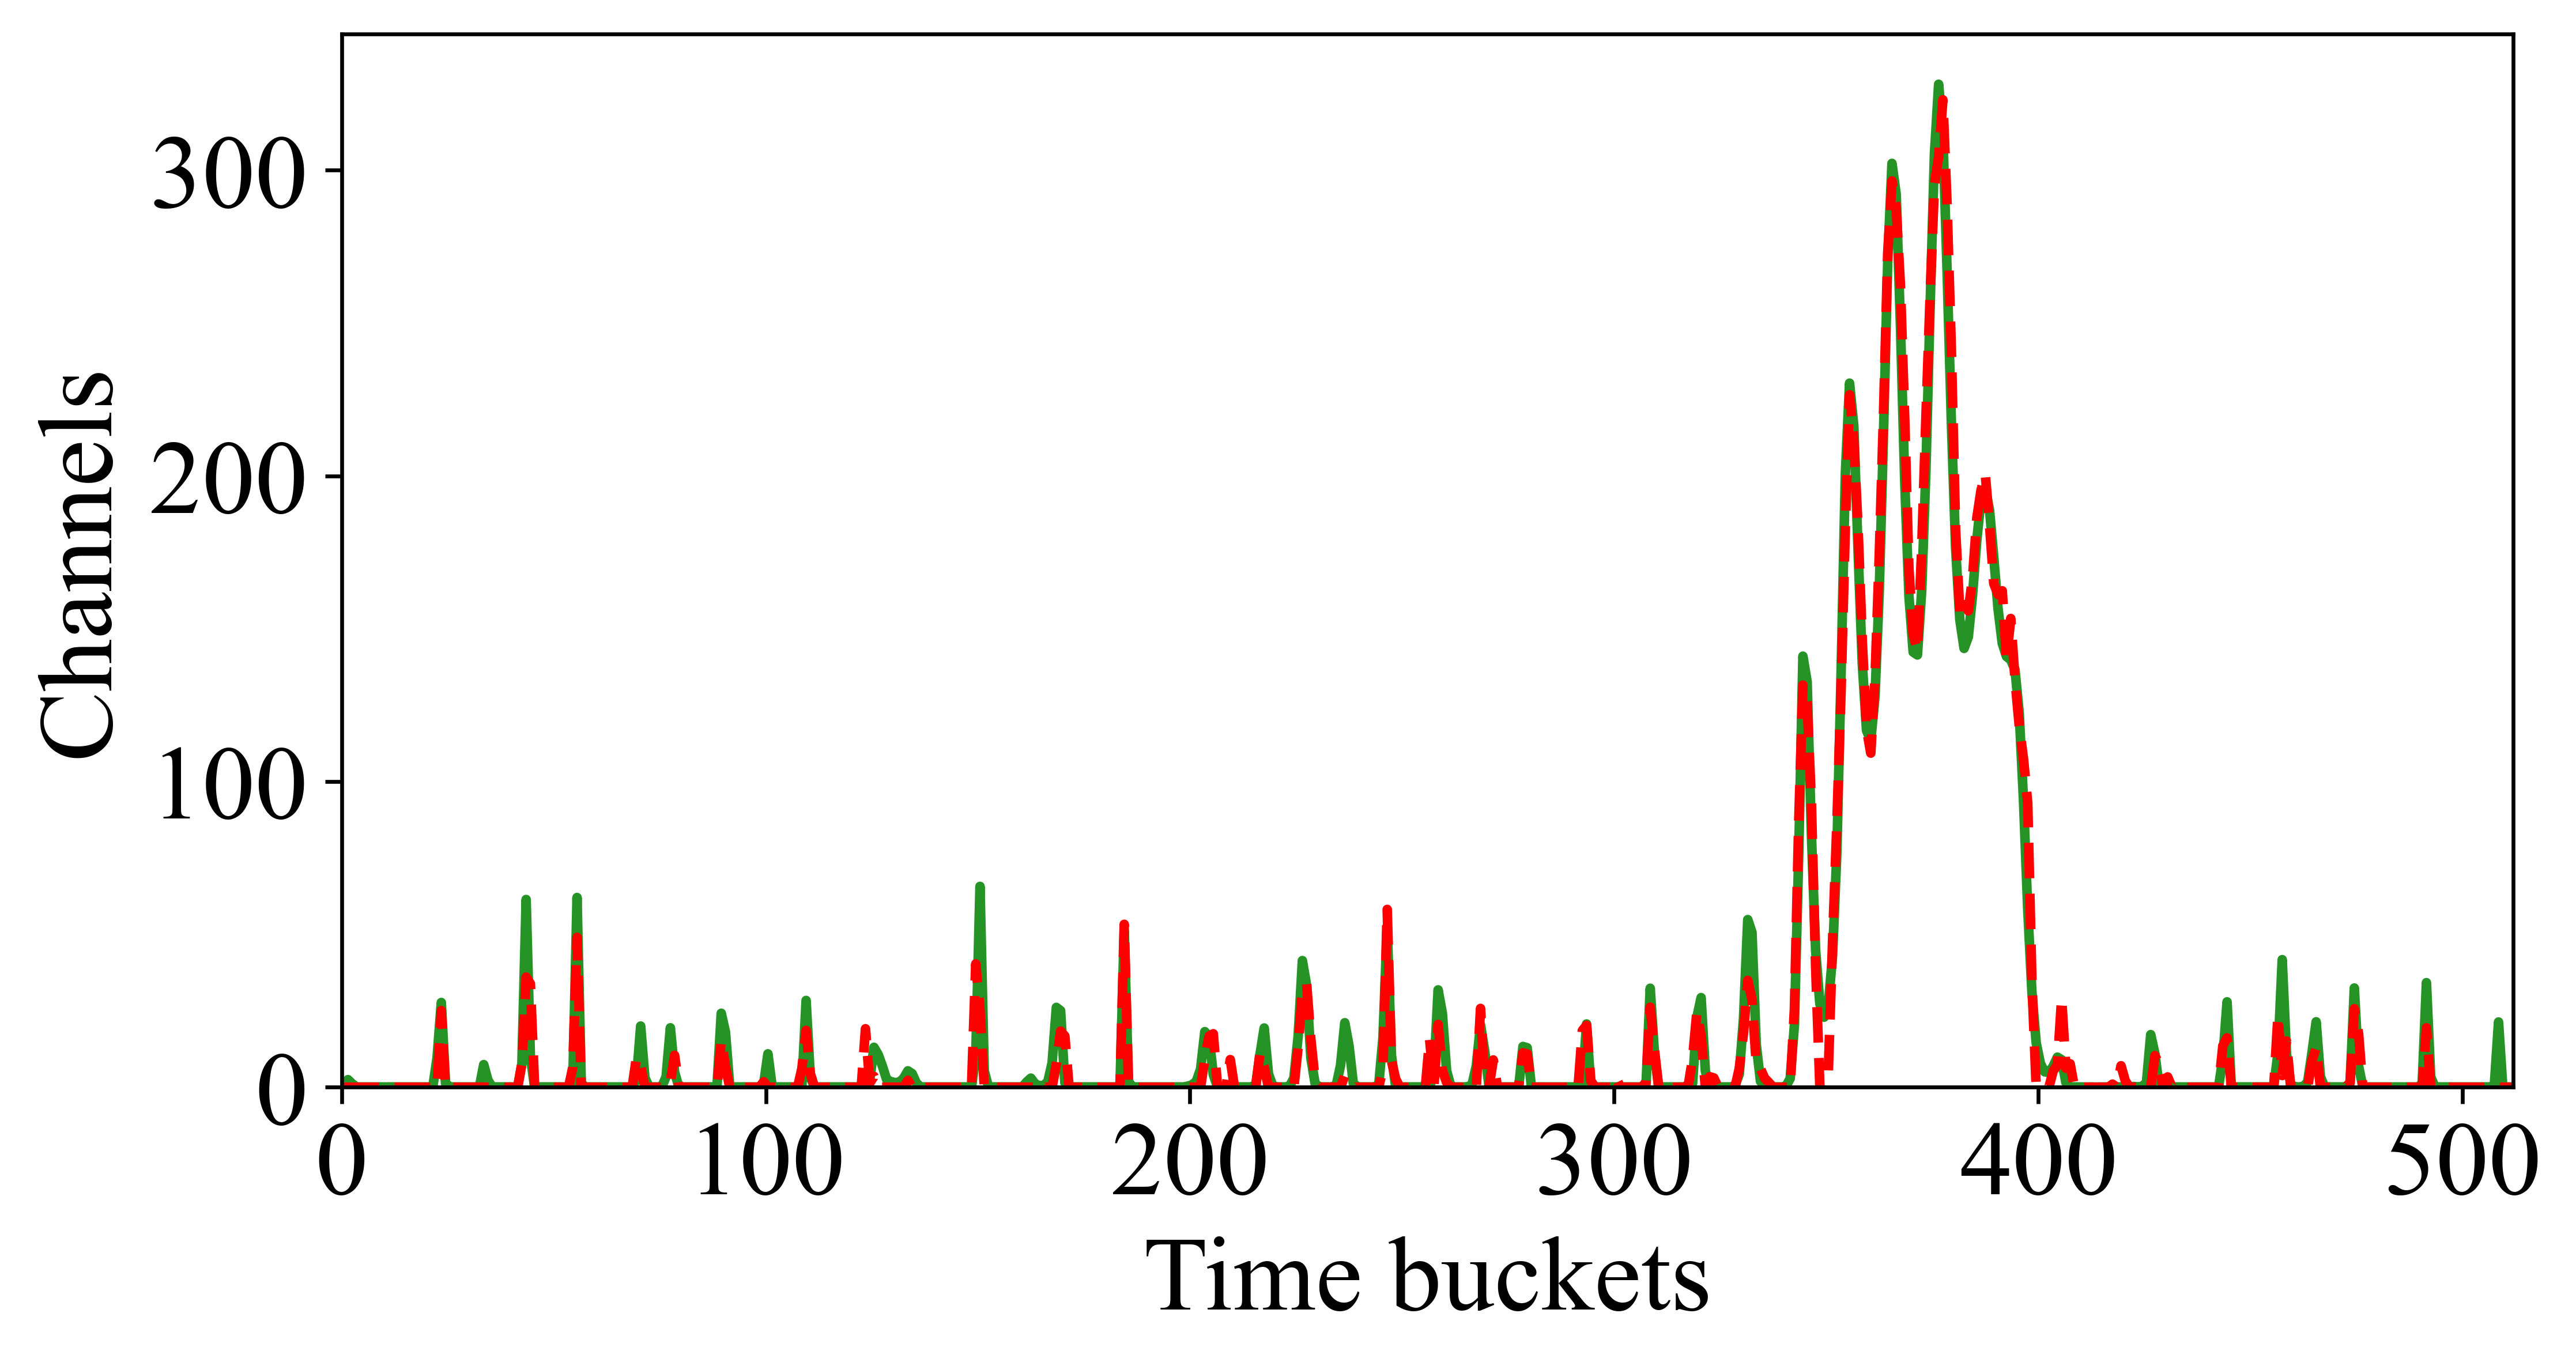
\includegraphics[scale=0.425]{figs/swbtd_3.png}
        \caption{}
        \label{subfig:std_ex3}
    \end{subfigure}%
    \hfill
    \begin{subfigure}[b]{0.465\textwidth}
        \centering
        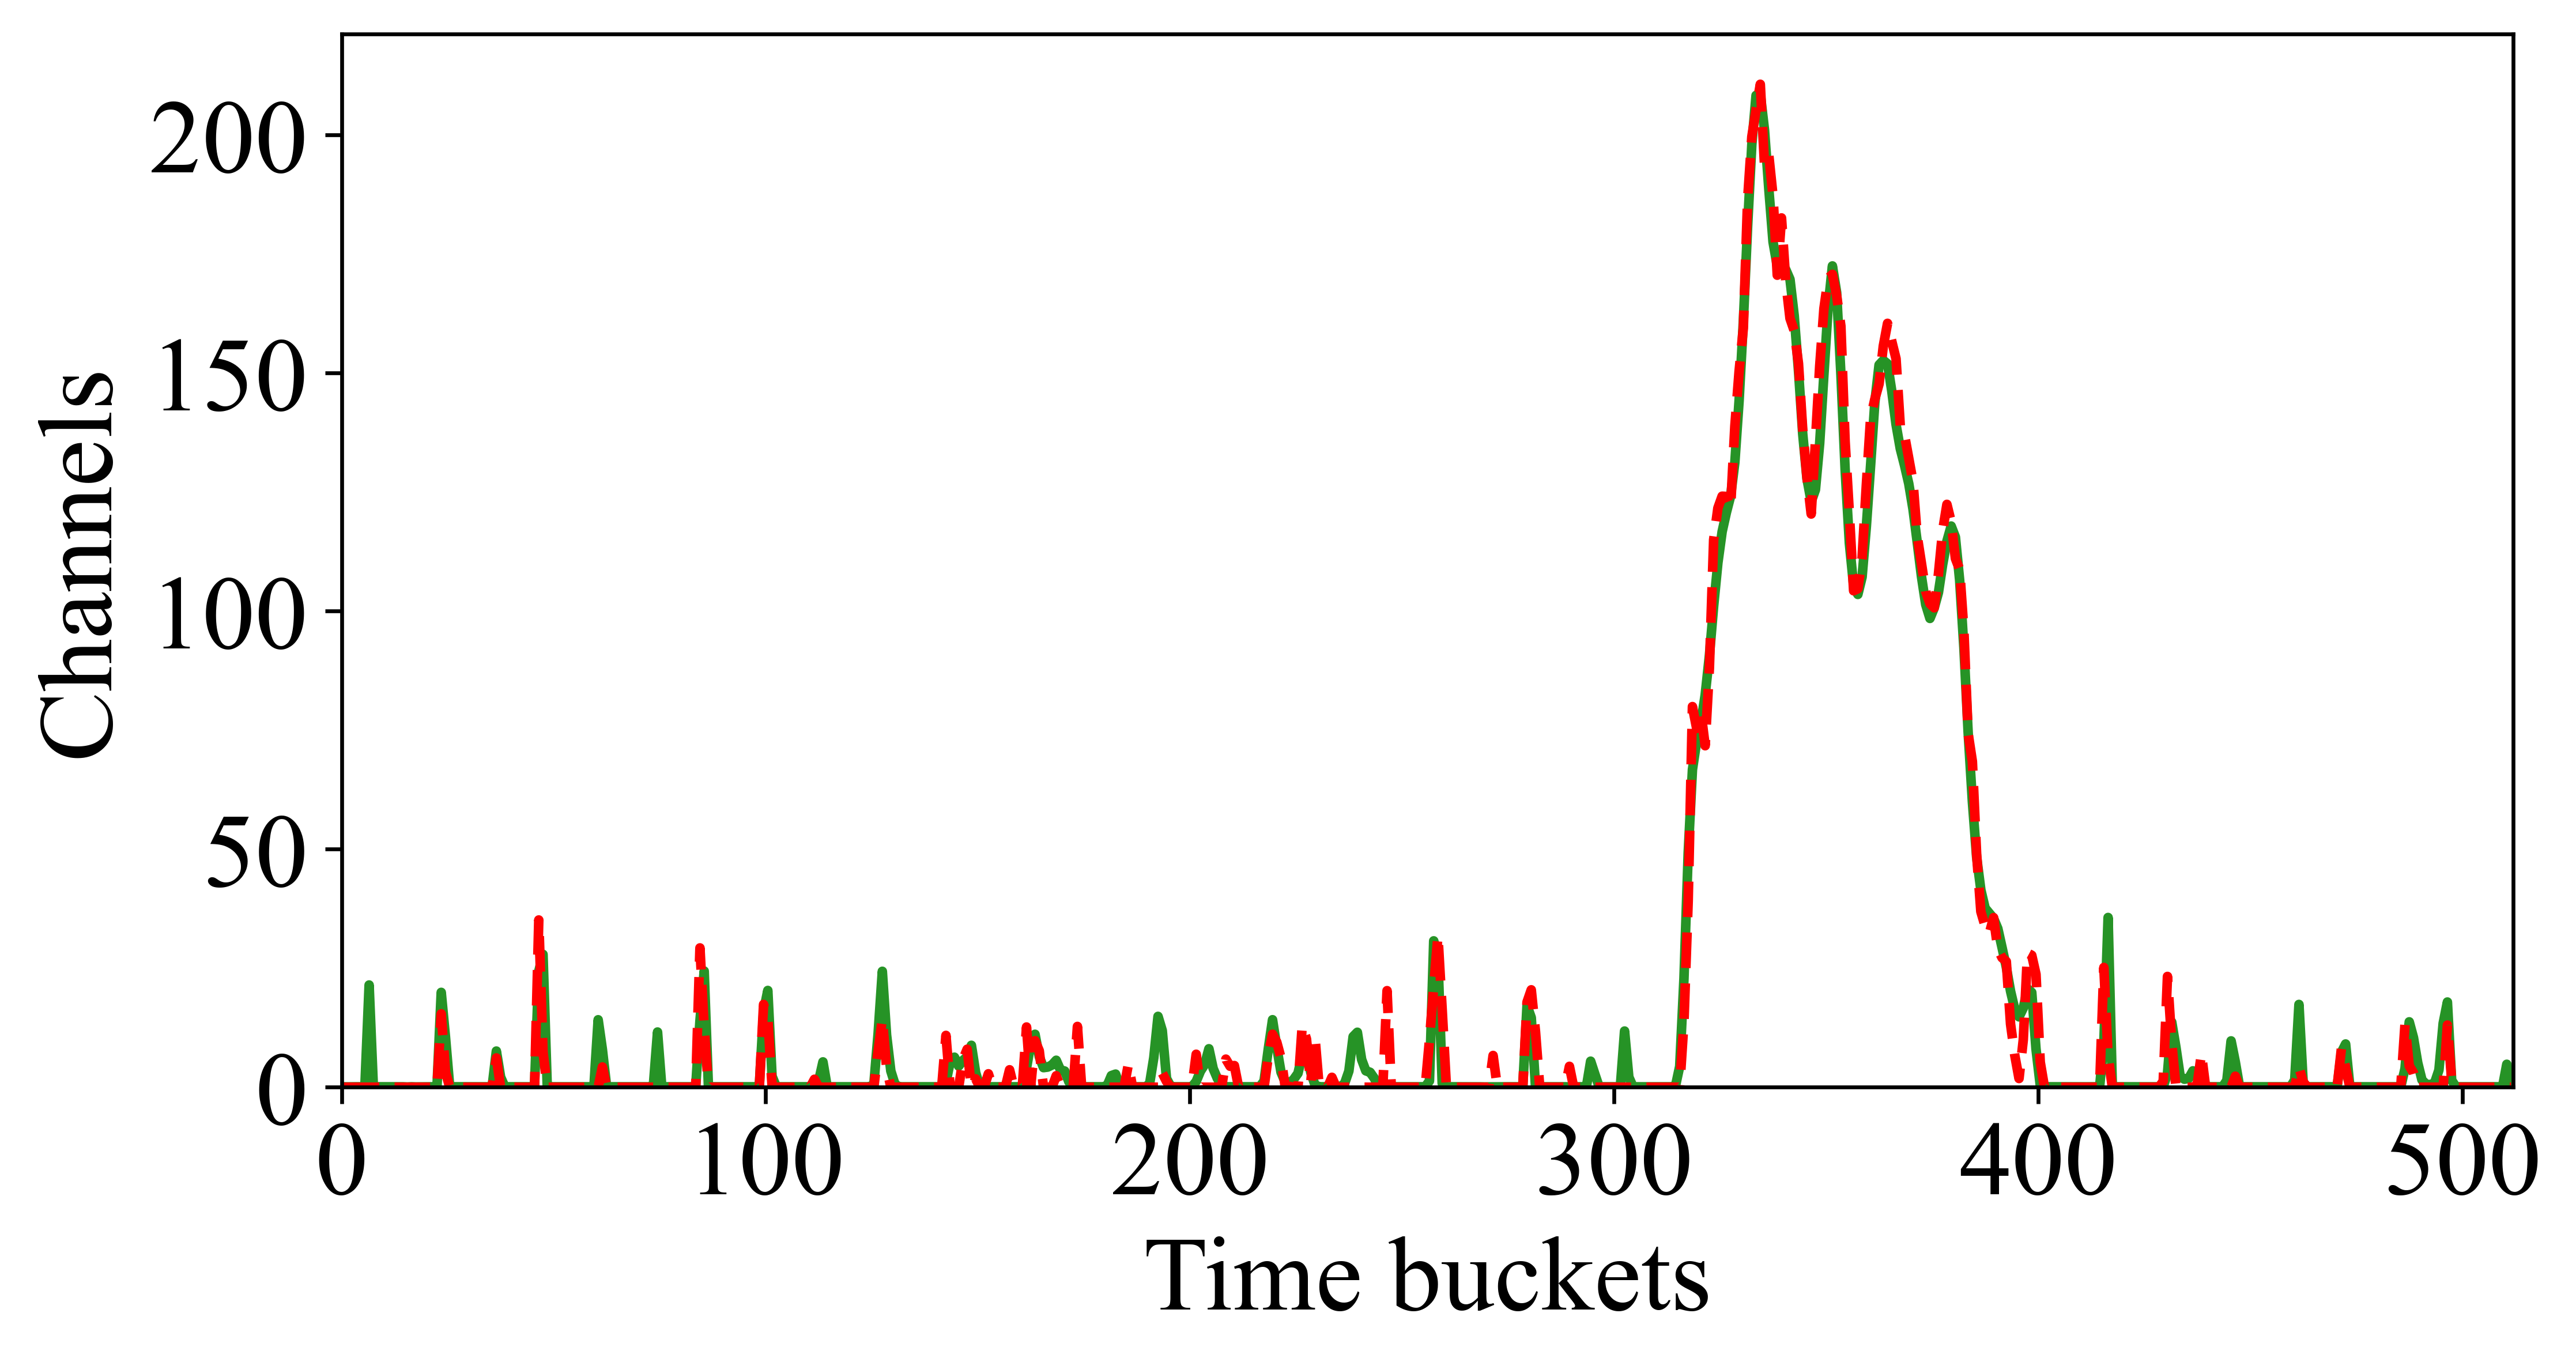
\includegraphics[scale=0.425]{figs/swbtd_4.png}
        \caption{}
        \label{subfig:std_ex4}
    \end{subfigure}
\caption{Exemplos de deconvolução da rede neural dada pela figura \ref{fig:arq_source_to_bkg}.}
\label{fig:std_examples}
\end{figure}

\par Com a rede neural para a deconvolução feita, a última etapa é a construção de uma rede neural para a identificação de picos, mostrada na \ref{subsec:pulso_ml_peaks}.

\subsection{Identificação de picos}\label{subsec:pulso_ml_peaks}

\par A última etapa dessa análise com \textit{machine learning} foi analisar possíveis soluções para a identificação de picos. Esse é um problema muito complexo, pois há uma variação muito grande na quantidade de picos por sinal e também há um desbalanço muito grande na quantidade de pontos comuns (aqueles que não são picos) e pontos que são picos. Por exemplo, caso haja um sinal que possui apenas um pico, deve-se identificar uma posição, dar o valor de saída como 1, por exemplo, dentre 512 pontos, onde 511 terão o valor de saída como 0. Caso a rede determine que todos os pontos são não picos, ainda assim a acurácia binária seria maior que 99\%. Isso é conhecido como desbalanço de classe\cite{inproceedings}.

\par Para corrigir esse desbalanço, foram acrescentados pontos simetricamente em torno do pulso, de forma que a somatória das amplitudes das regiões é equivalente a carga $Q$ acumulada no ponto. Isso faz com que não seja preciso identificar um único ponto, mas sim uma região em torno do pico. Com isso podemos nos basear na ideia de segmentar o sinal para destacar regiões de interesse\cite{aly2011research}. Segmentar significa ter uma rede neural com a saída com o mesmo tamanho do vetor de entrada (512) e saída com valores entre 0 e 1, onde 1 indica uma região com um pico e 0 não. A figura \ref{fig:n_peaks_exs} mostra um exemplo de um sinal após a deconvolução onde há os picos identificados com o algoritmo \textit{peak\_finder} e os pontos acrescentados simetricamente em torno dos picos para representar as regiões dos pulsos.

% \par Para resolver esse problema podemos nos basear na ideia de recortar regiões de interesse, como feito pela rede U-Net\cite{unet}. Recortar regiões significa, nesse caso, ter uma rede neural com a saída com o mesmo tamanho do vetor de entrada (512) e saída com valores entre 0 e 1, onde 1 indica uma região com um pico e 0 não. Como temos as posições dos picos, basta acrescentar pontos simetricamente em torno do pulso. A figura \ref{fig:n_peaks_exs} mostra um exemplo de um sinal após a deconvolução onde há o pico detectado e os pontos acrescentados para representar a região do pulso.

\begin{figure}[H]
    \centering
    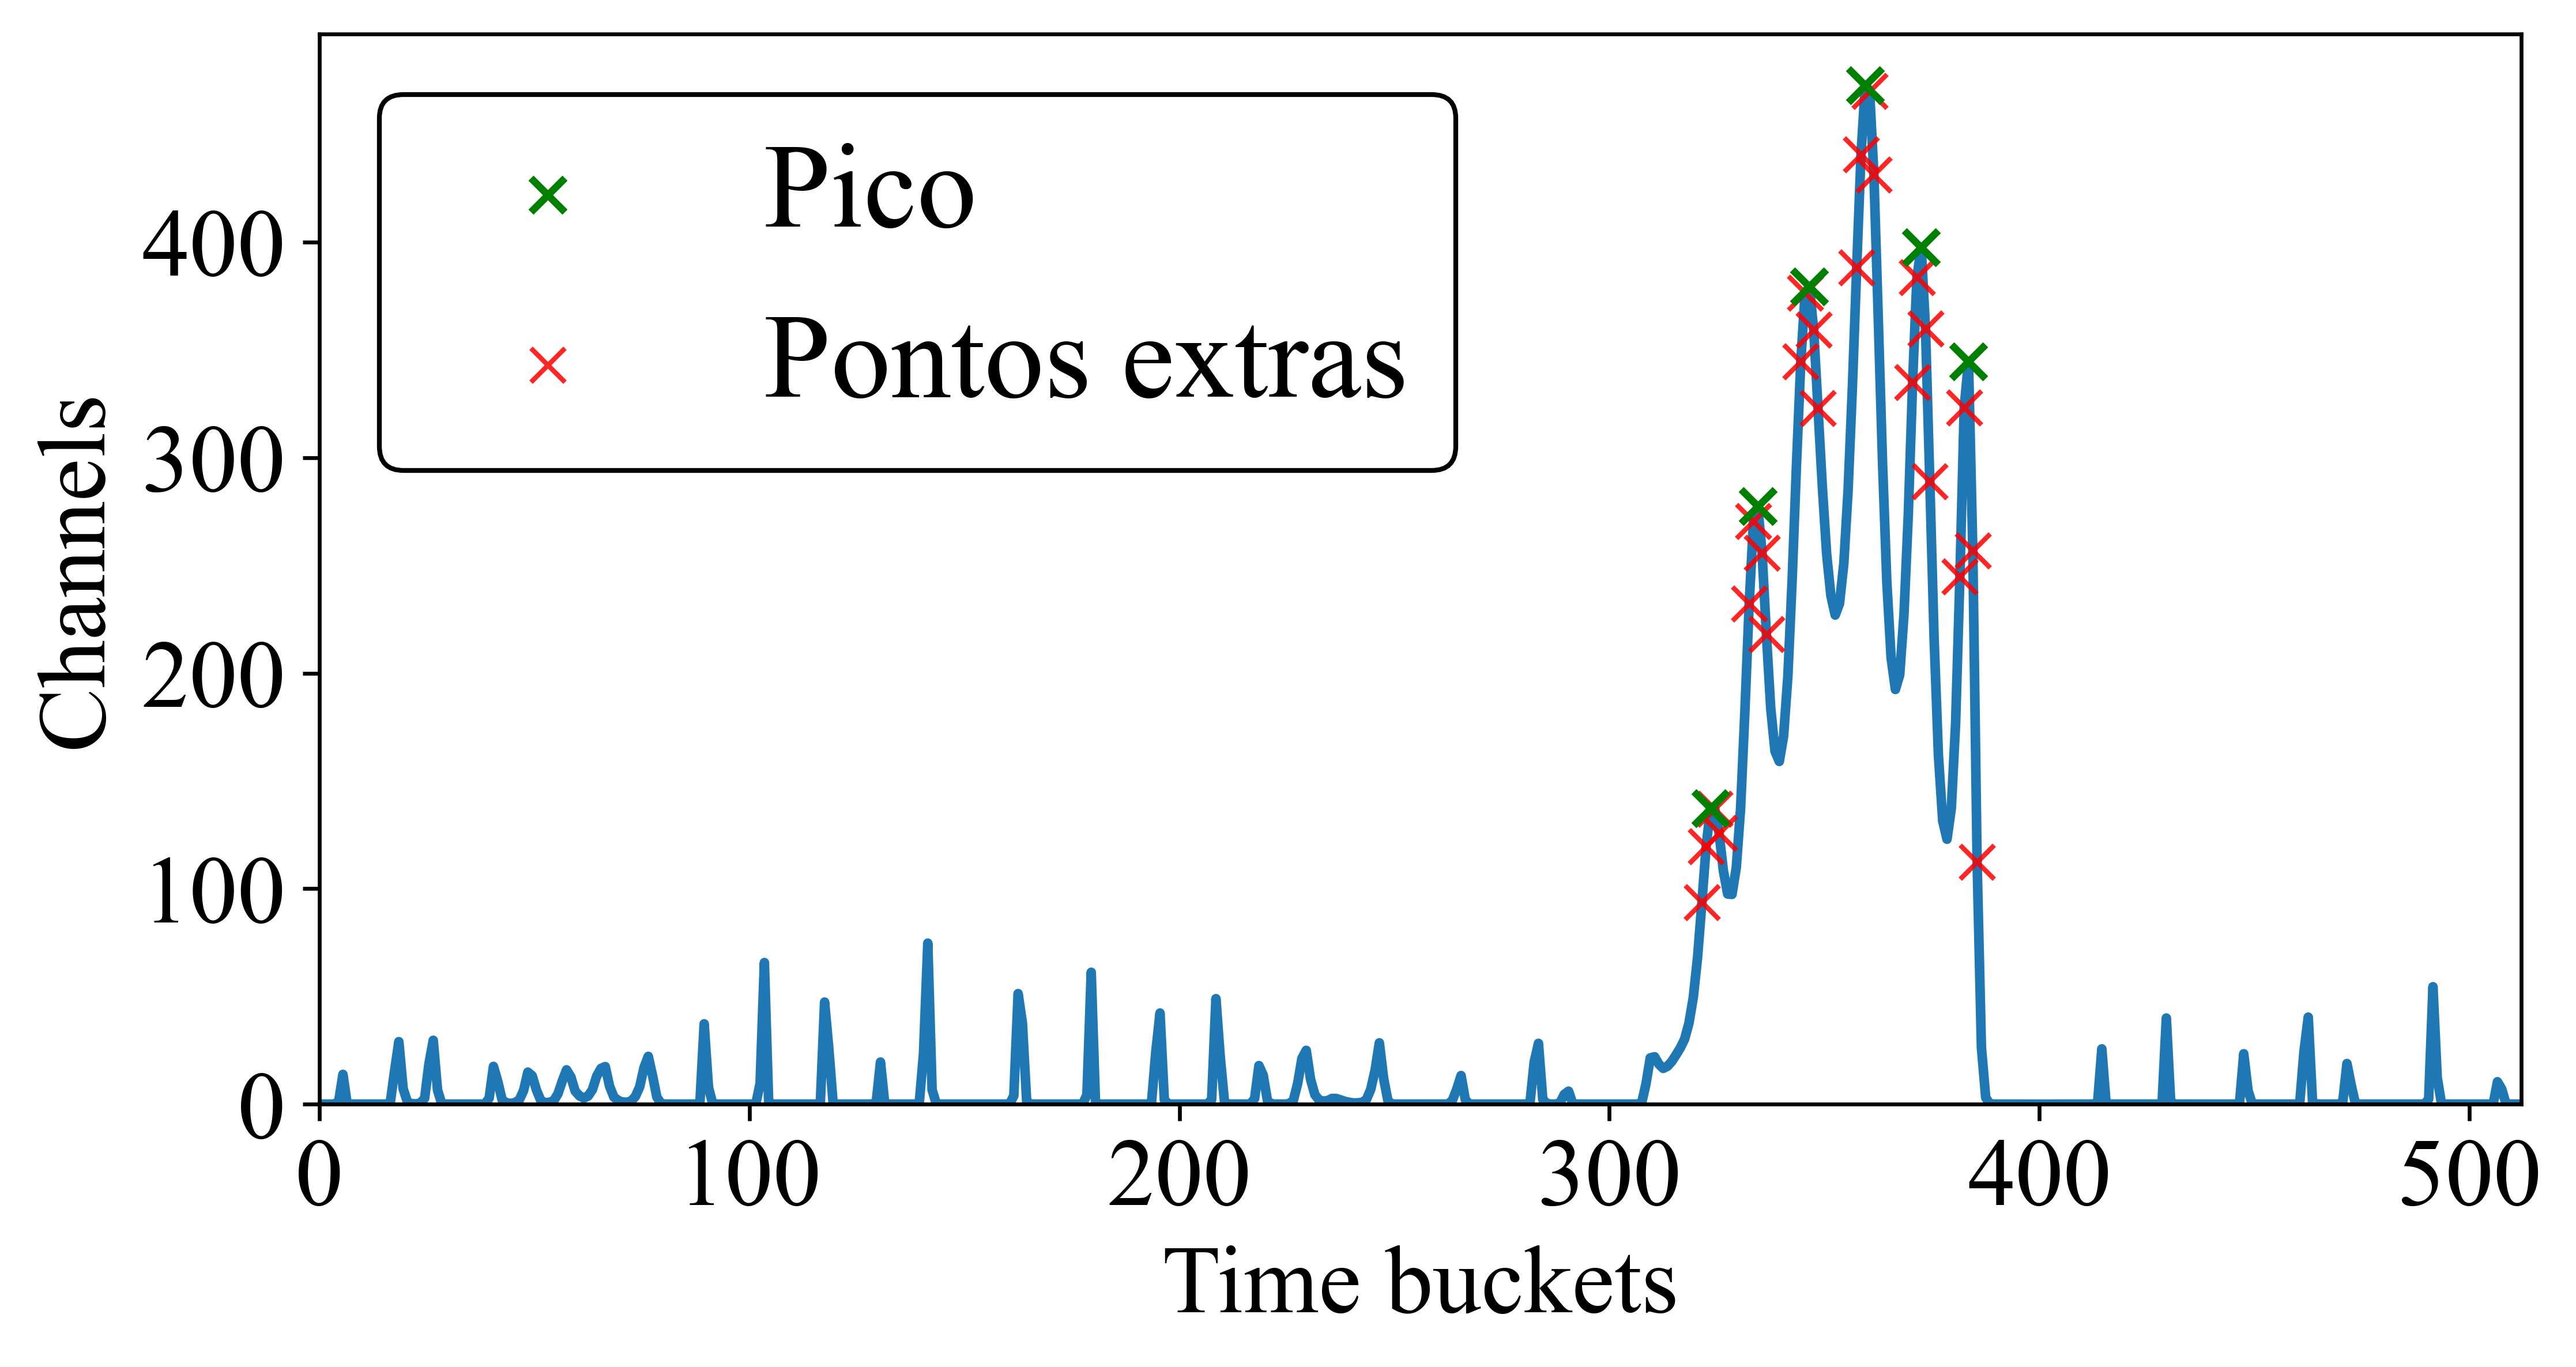
\includegraphics[scale = 0.6]{figs/np_ex1.png}
    \caption{Sinal após a deconvolução que mostra o pico identificado mais os pontos adicionais que irão facilitar o trabalho da rede neural (evitar o desbalanço de classe). Foram acrescentados 2 pontos à esquerda e à direita.}
    \label{fig:n_peaks_exs}
\end{figure}

\par A rede construída é a sequência de uma convolução com \textit{kernel} de tamanho 13 e \textit{same padding} seguida de \textit{Max-Pooling} e uma \textit{fully-connected} com função de ativação sigmoide, possuindo um total de 263.104 parâmetros treináveis. Para o treino foram usados sinais que possuíam entre 1 e 6 picos, resultantes da saída do algoritmo \textit{peak\_finder} do \textit{SciPy}, o que resultou em 120.024 de dados para o treino e 30.006 para validação. A escolha pelos picos identificados pelo \textit{peak\_finder} ao invés do algoritmo de identificação do TSpectrum é pela maior flexibilidade de ajuste fino do algoritmo, tornando a identificação de picos muito melhor\cite{FORTINO2022166497}. A função custo escolhida foi a \textit{binary cross-entropy} (dada pela equação \ref{eq:binary_cross_entropy}), o otimizador o \textit{ADAM} com \textit{learning rate} de 0.001. A métrica utilizada foi a acurácia binária. O treino também foi realizado por uma GPU NVIDIA Tesla P100 e durou cerca de 8 minutos com 12 \textit{epochs}. A arquitetura da rede está na figura \ref{fig:arq:n_peaks} e os resultados do treino estão na figura \ref{fig:n_peaks_results}.

\begin{figure}[H]
    \centering
    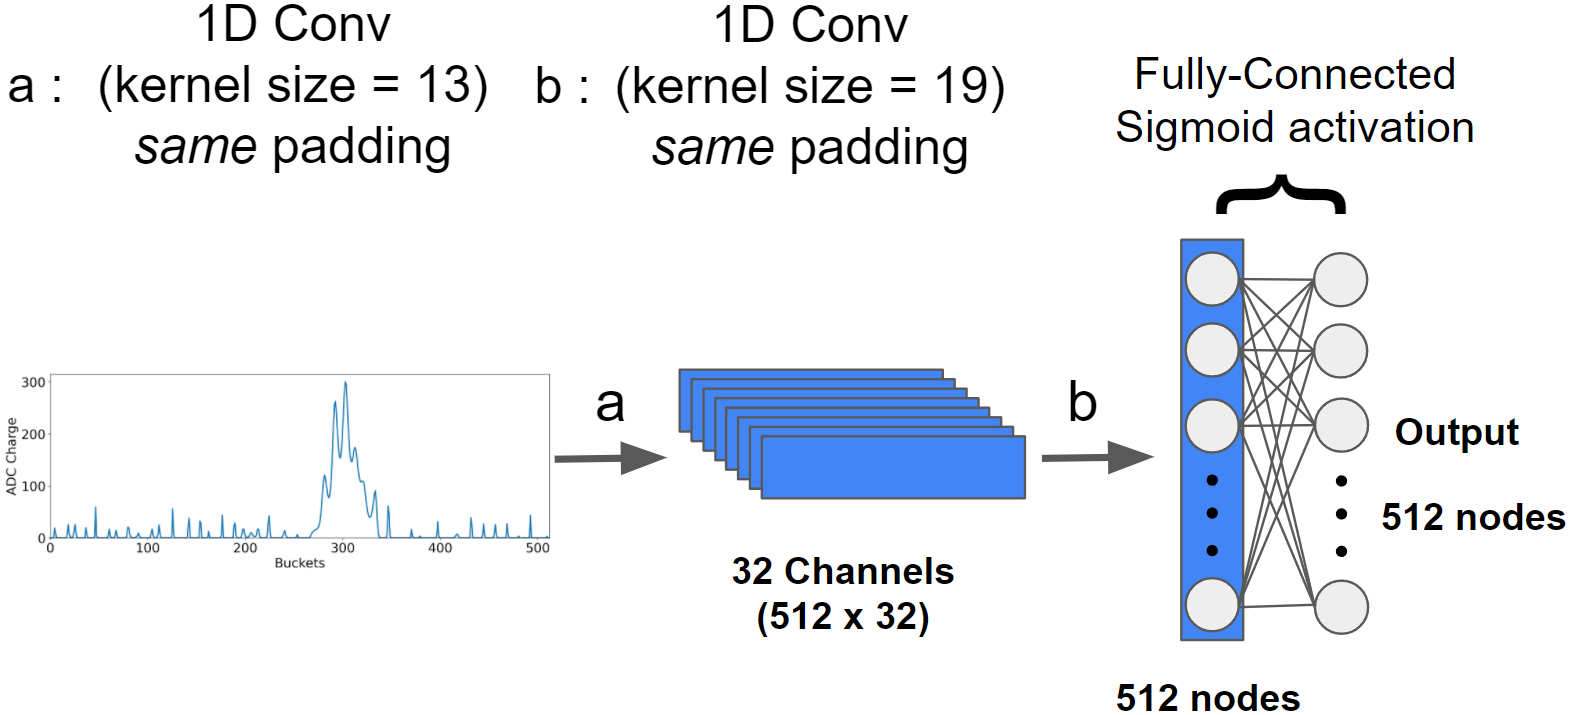
\includegraphics[scale = 0.35]{figs/n_peaks.png}
    \caption{Arquitetura da rede neural que faz o recorte das regiões com picos. O vetor de entrada deve ter dimensionalidade 512 x 1.}
    \label{fig:arq:n_peaks}
\end{figure}

\begin{figure}[H]
\centering
    \begin{subfigure}[t]{0.49\textwidth}
        \centering
        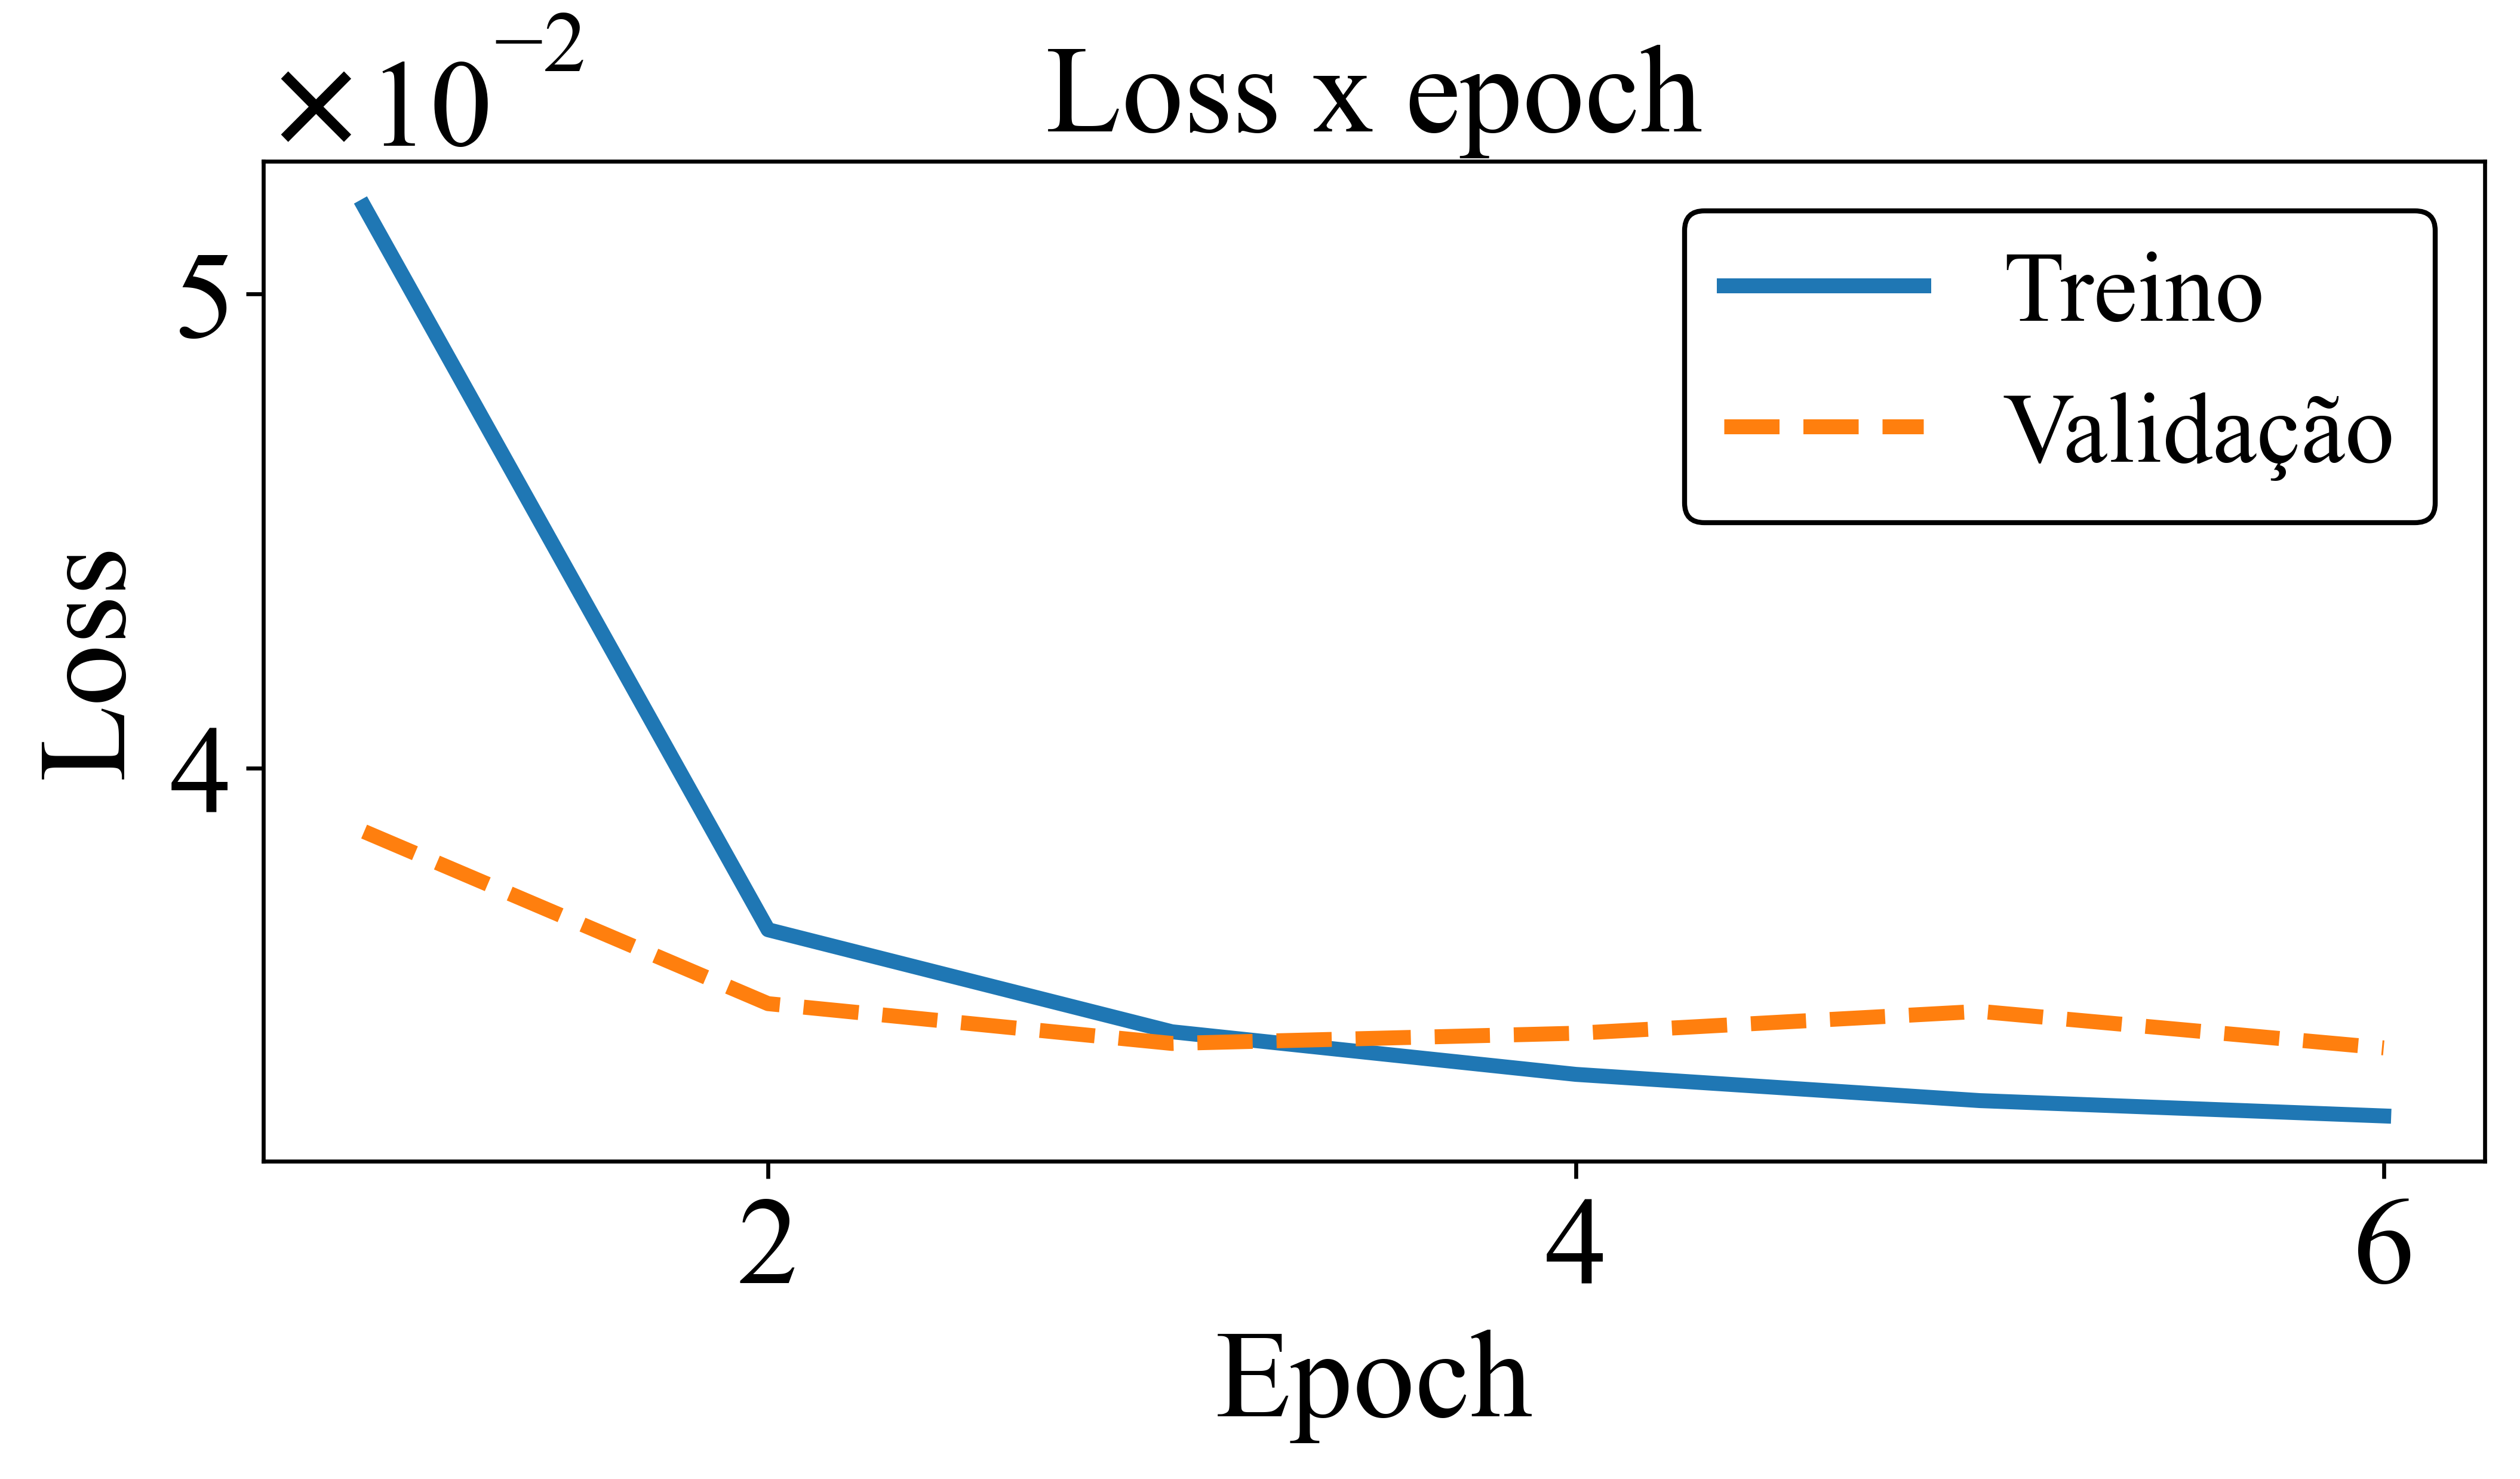
\includegraphics[scale=0.42]{figs/n_peaks_loss.png}
        \caption{\textit{Loss} dos dados de treino (linha contínua) e dos dados de validação (linha tracejada) em função da \textit{epoch}.}
        \label{subfig:n_peaks_loss}
    \end{subfigure}%
    \hfill
    \begin{subfigure}[t]{0.46\textwidth}
        \centering
        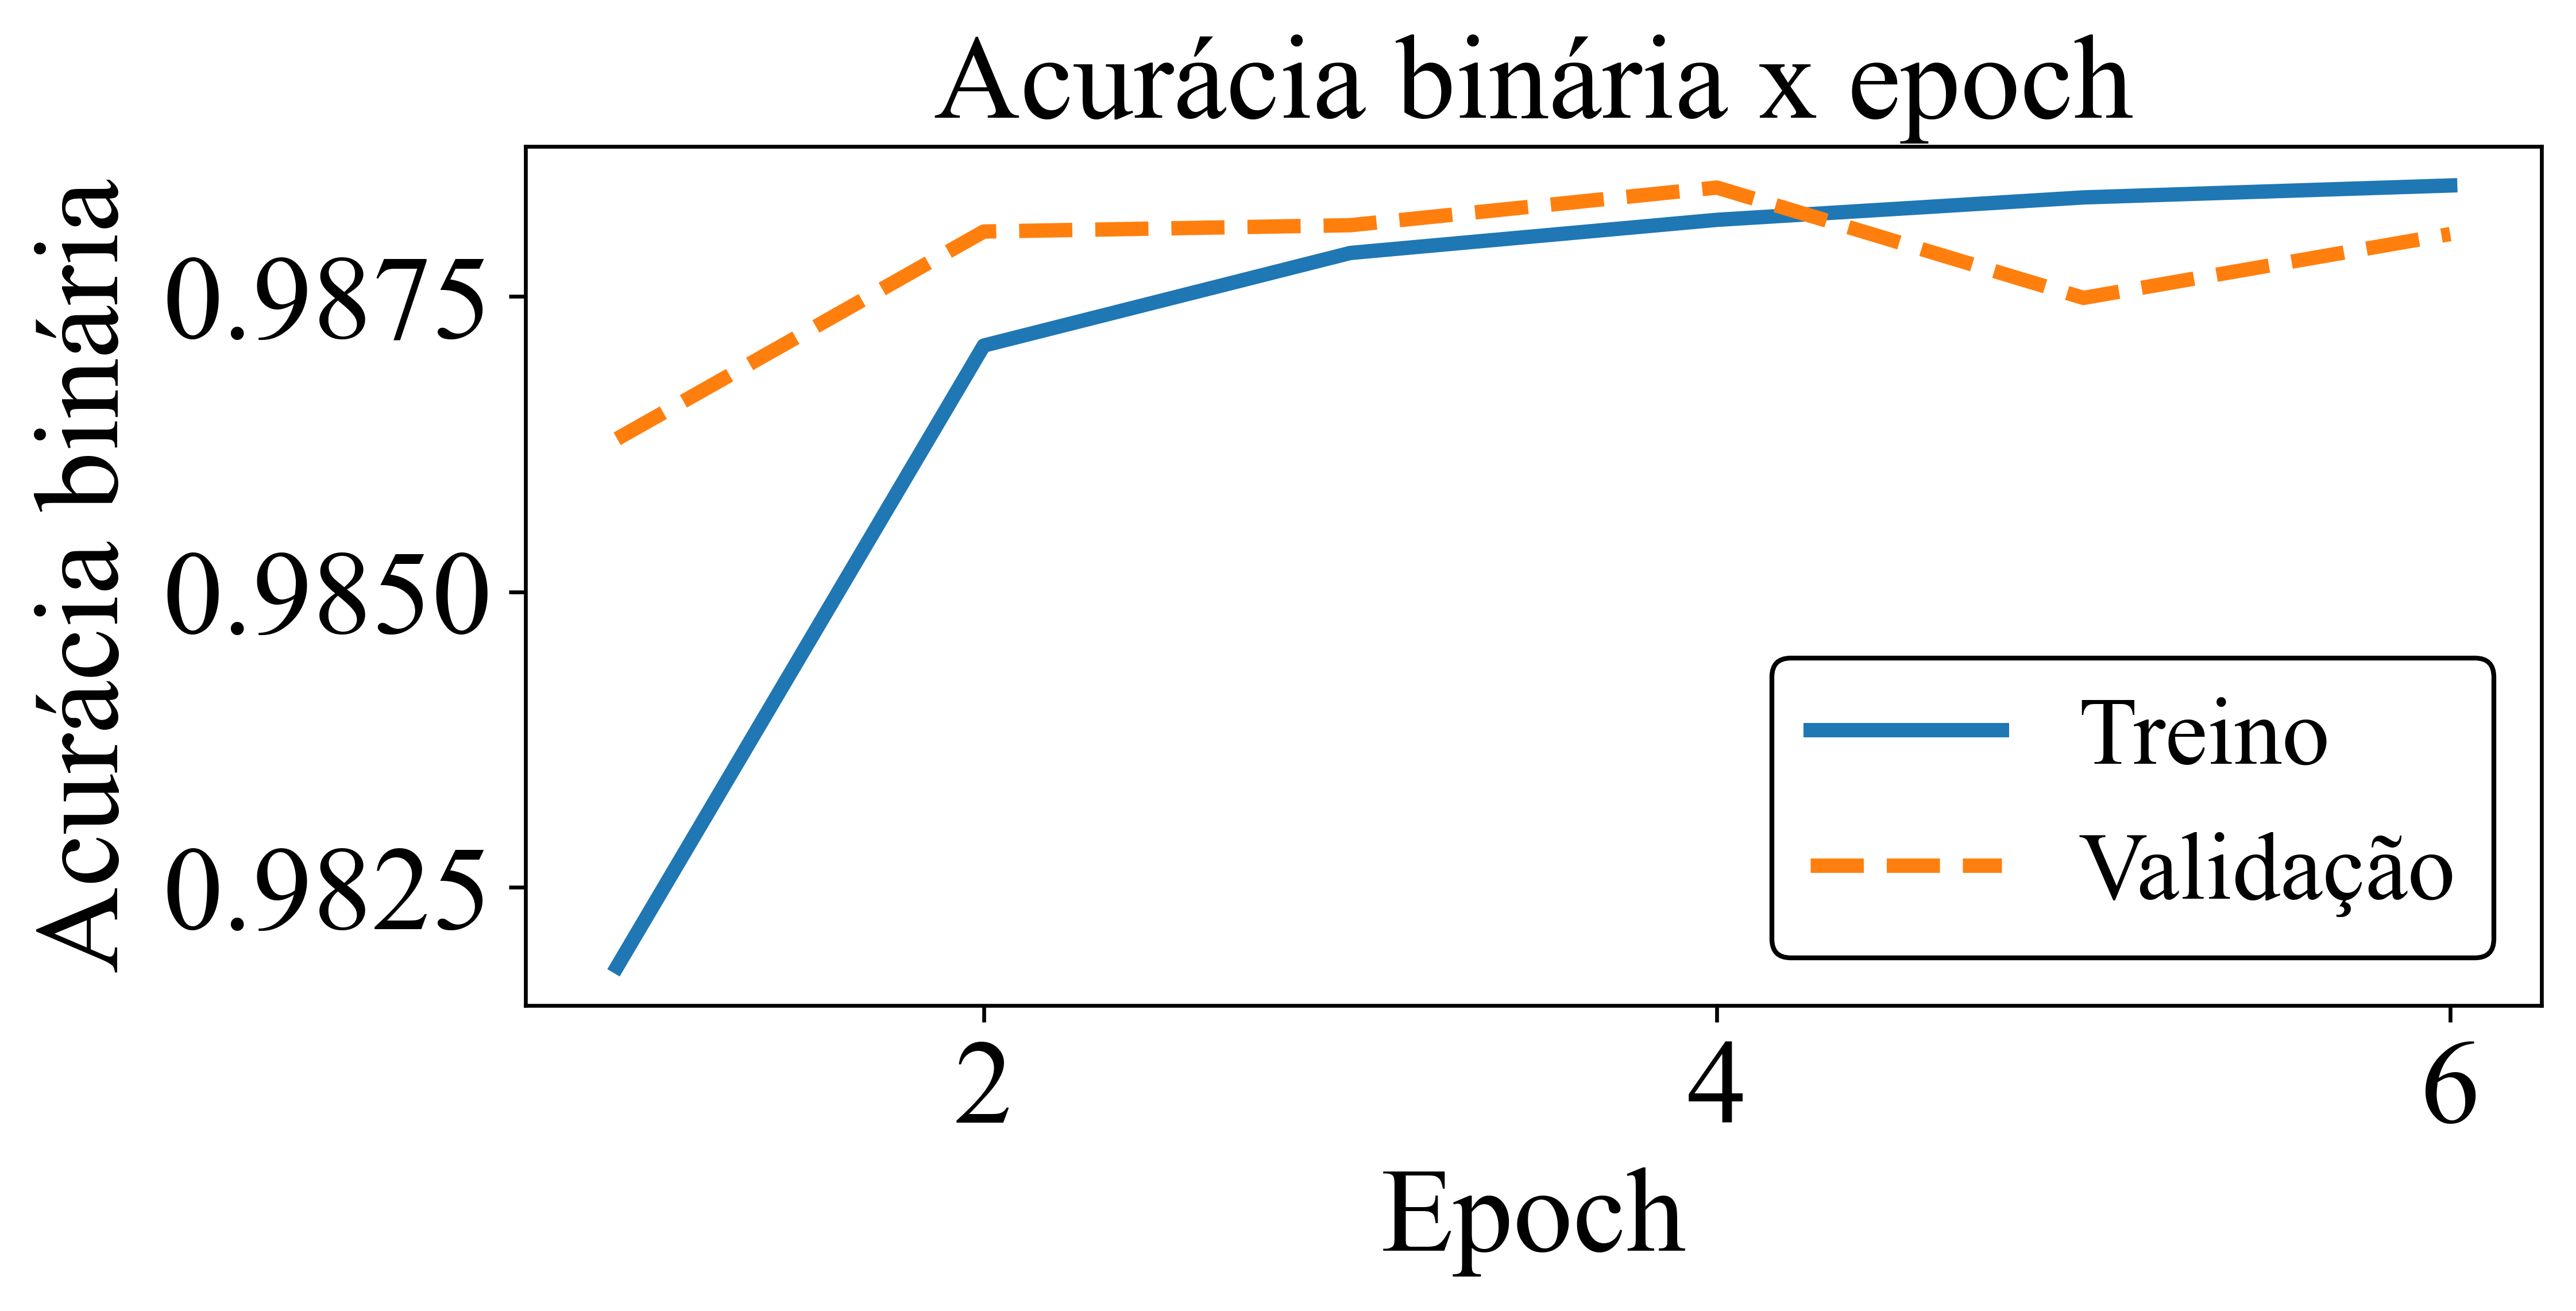
\includegraphics[scale=0.42]{figs/n_peaks_metric.png}
        \caption{Acurácia binária dos dados de treino (linha contínua) e dos dados de validação (linha tracejada) em função da \textit{epoch}.}
        \label{subfig:n_peaks_metric}
    \end{subfigure}
\caption{Resultados do treino da rede neural dada pela figura \ref{fig:arq:n_peaks}.}
\label{fig:n_peaks_results}
\end{figure}

\par A saída da rede neural é um vetor de tamanho 512 com valores entre 0 e 1, onde valores maiores que 0.5 são considerados como pertencentes à um pulso. Com as regiões identificadas podemos fazer uma média ponderada com o espectro de entrada para achar o centroide. O tempo de processamento da rede neural é de 150.030 sinais em cerca de 4.11 segundos (aproximadamente 36.500 sinais por segundo). Para determinar os picos a partir da saída da rede neural, o tempo é de aproximadamente 4.3 segundos, onde o algoritmo pode ser ainda mais rápido se for paralelizado. Resultados para picos identificados pela rede neural em comparação com o algoritmo \textit{peak\_finder} estão na figura \ref{fig:exs_n_peaks}.

\begin{figure}[H]
\centering
    \begin{subfigure}[b]{0.49\textwidth}
        \centering
        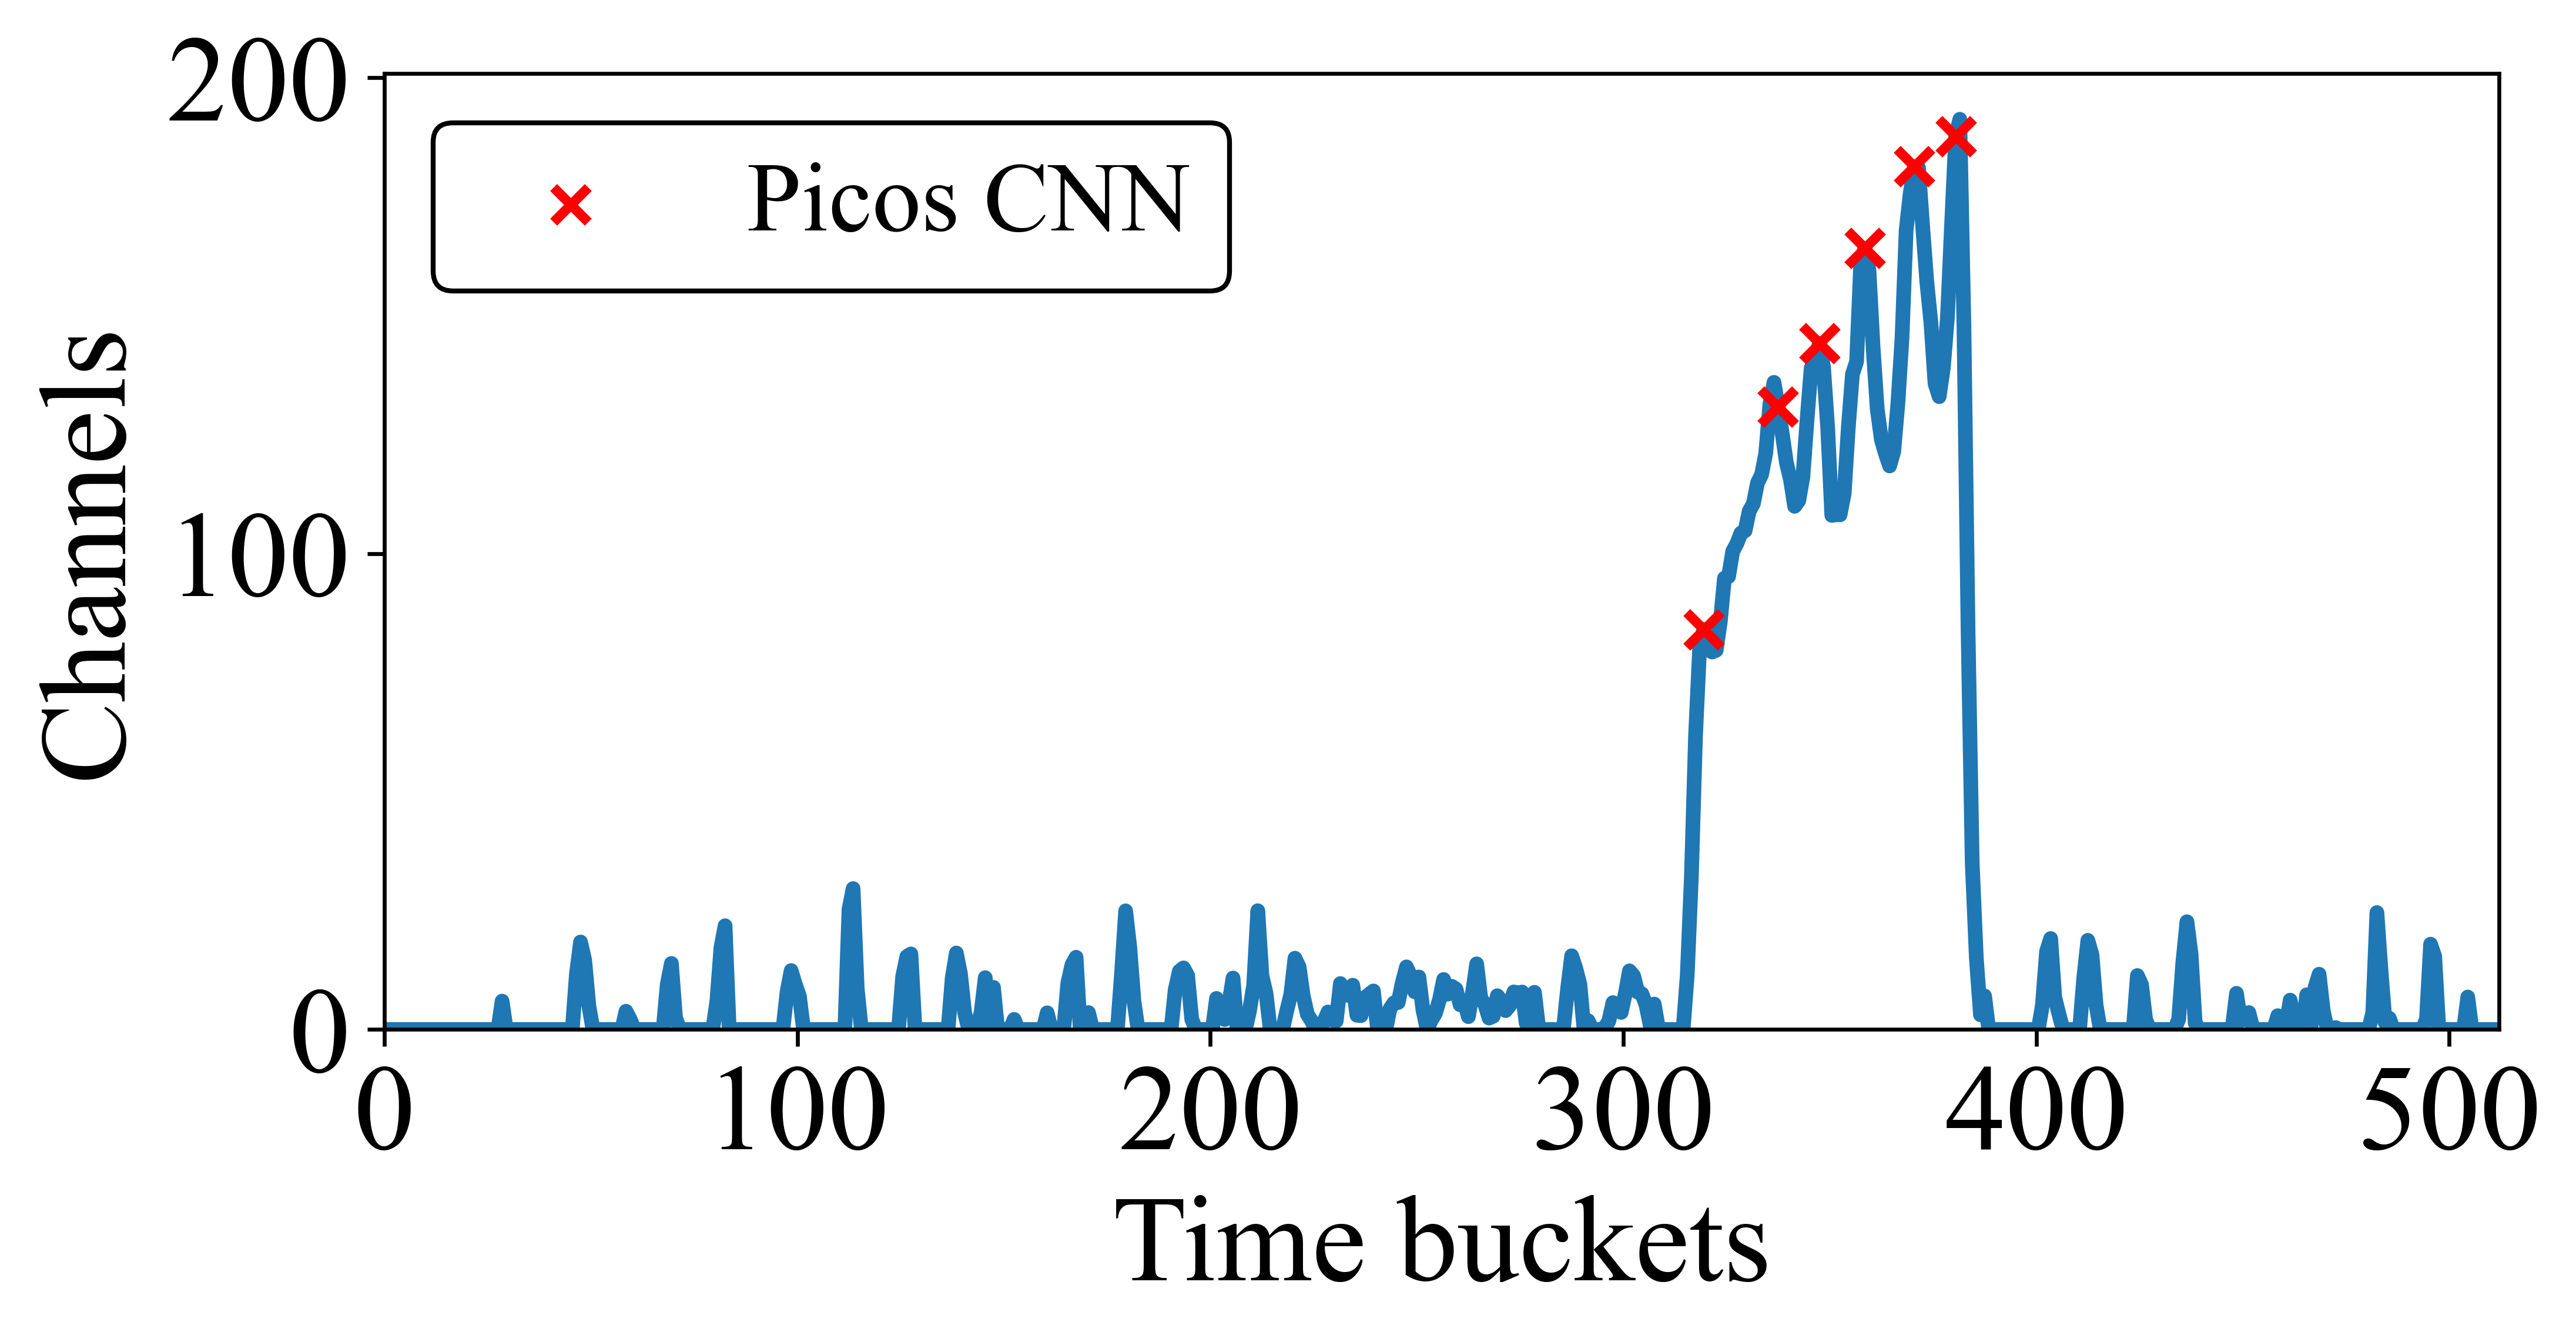
\includegraphics[scale=0.425]{figs/np_exs1.png}
        \caption{}
        \label{subfig:exs_n_peaks_1}
    \end{subfigure}%
    \hfill
    \begin{subfigure}[b]{0.465\textwidth}
        \centering
        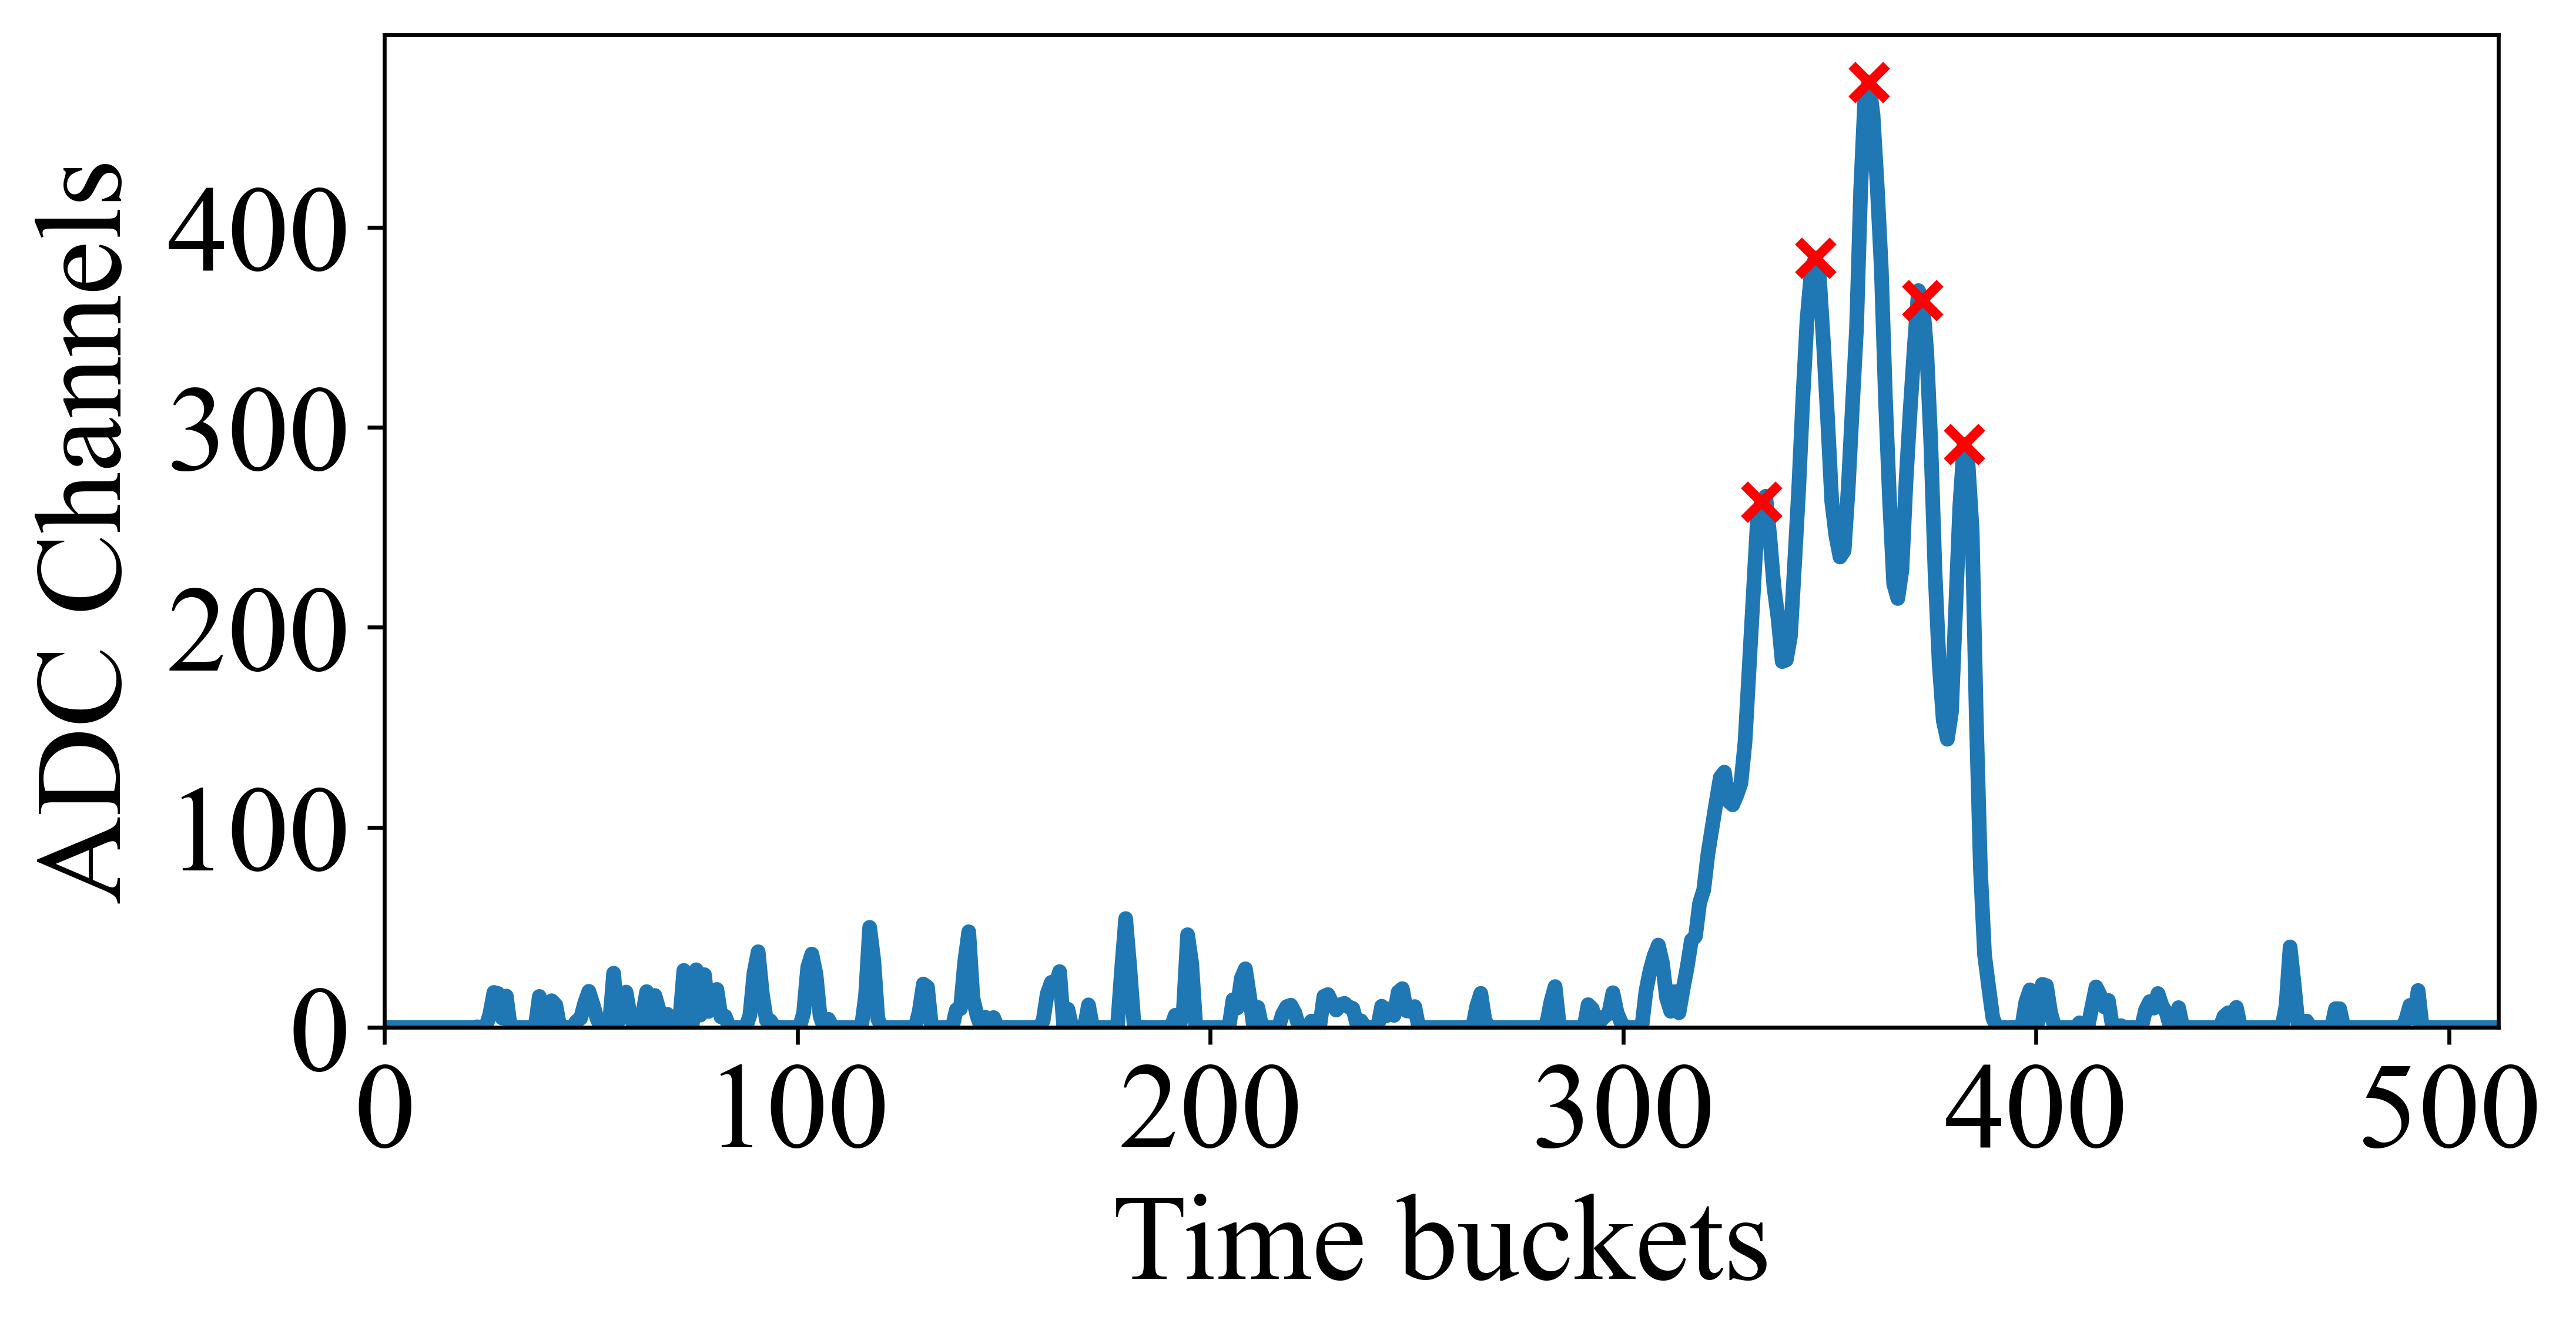
\includegraphics[scale=0.425]{figs/np_exs2.png}
        \caption{}
        \label{subfig:exs_n_peaks_2}
    \end{subfigure}
    \begin{subfigure}[b]{0.49\textwidth}
        \centering
        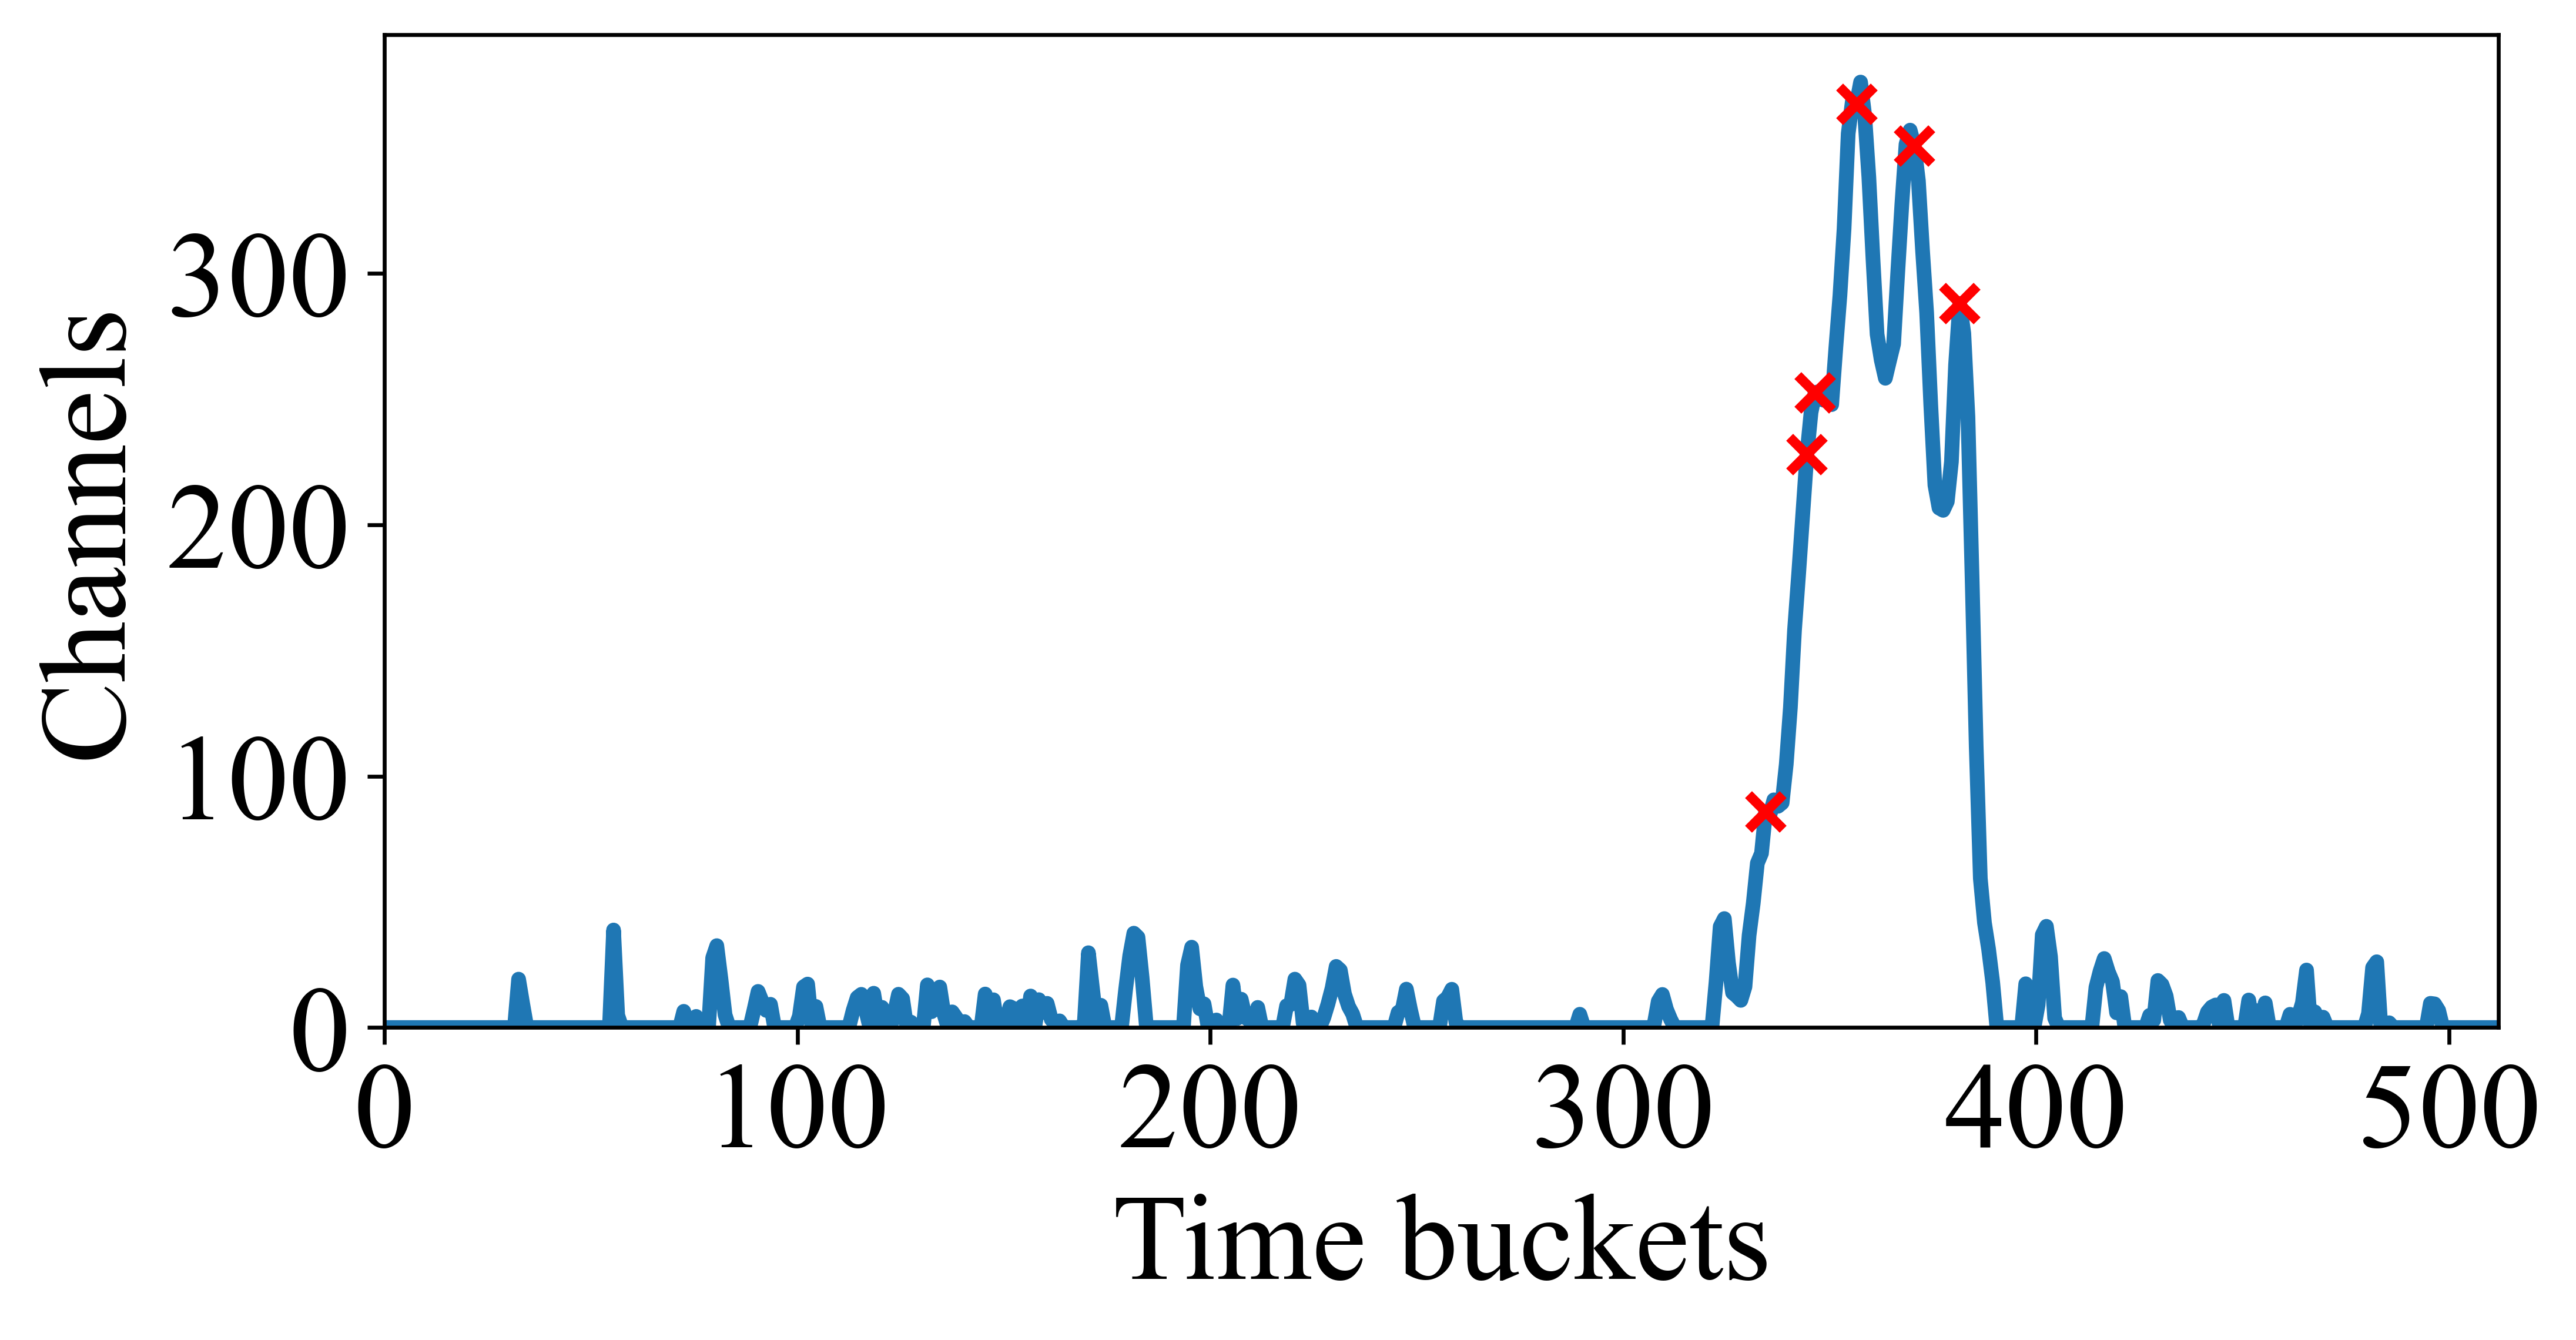
\includegraphics[scale=0.425]{figs/np_exs3.png}
        \caption{}
        \label{subfig:exs_n_peaks_3}
    \end{subfigure}%
    \hfill
    \begin{subfigure}[b]{0.465\textwidth}
        \centering
        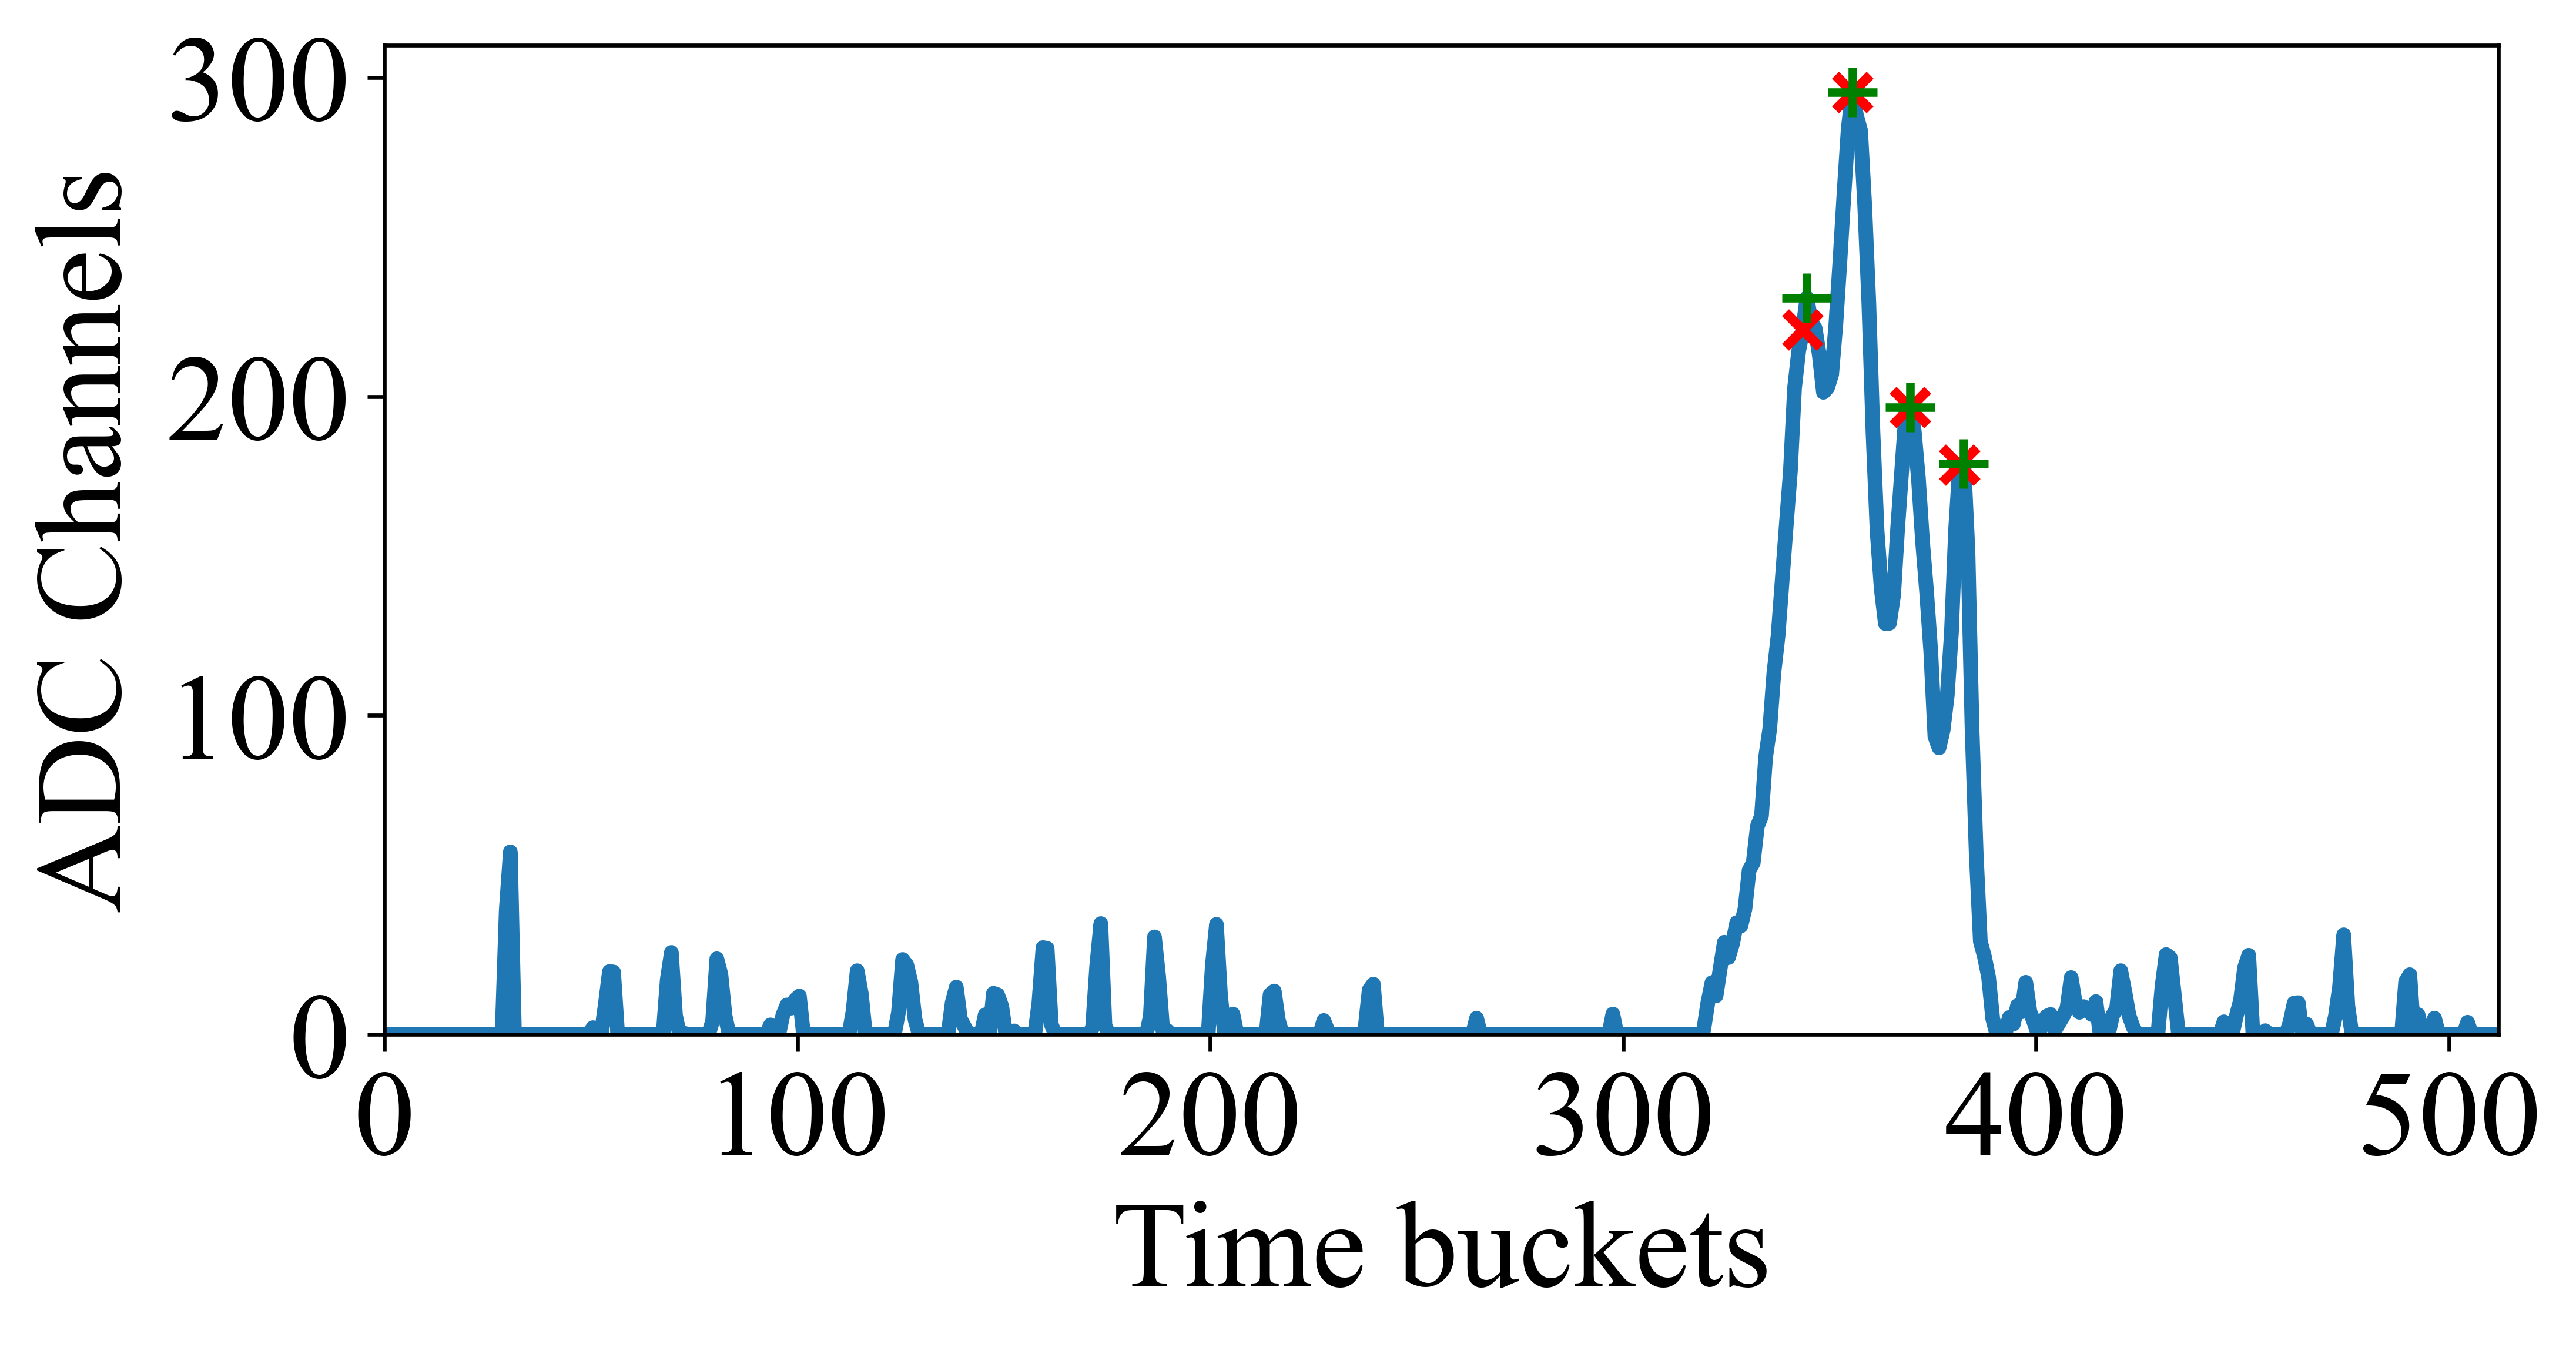
\includegraphics[scale=0.425]{figs/np_exs4.png}
        \caption{}
        \label{subfig:exs_n_peaks_4}
    \end{subfigure}
\caption{Exemplos de identificação de picos usando a rede neural, em comparação com a identificação feita pelo algoritmo presente no SciPy, mostrada na figura \ref{fig:arq:n_peaks}. Os centroides identificados pela rede neural estão em vermelho, e os centroides identificados pelo SciPy estão em verde. Em azul está o espectro sem fundo após a deconvolução, resultantes }
\label{fig:exs_n_peaks}
\end{figure}

\par Para determinar carga acumulada $Q_i$ de cada ponto associado à cada centroide $i$, foi usada a relação

\begin{equation}\label{eq:carga_acumulada_ml}
	Q_i = \sum_{i - 2}^{i + 2}f(t_i)\alpha_\sigma,
\end{equation}

\par onde $f(t_i)$ é a amplitude do espectro no \textit{time bucket} $t$ da posição $i$ e $\alpha_\sigma$ é uma constante real para calibrar o valor da área em função do sigma dos pulsos, que foi determinado empiricamente como $\alpha_\sigma$ = 1.2.

\par Com as três redes neurais criadas, é necessário verificar o acoplamento das redes, a fim de analisar a qualidade dos algoritmos e verificar os tempos de execução, para comparar com os algoritmos discutidos nas subseções \ref{subsec:pulses_baseline} e \ref{subsec:pulses_deconv}.


\subsection{Acoplando as redes neurais}

%\par Com a rede que prevê o fundo e a que faz a deconvolução funcionando podemos agora testar se acopladas elas geram resultados satisfatórios, verificando a qualidade da detecção de picos.
\par Usando novamente o TensorFlow 2 pode-se carregar as redes neurais discutidas nas subseções \ref{subsec:pulso_ml_fundo}, \ref{subsec:pulso_ml_deconv} e \ref{subsec:pulso_ml_peaks}, já treinadas e usar como se fosse uma única rede neural. Acoplando as três arquiteturas, temos a nova arquitetura mostrada na figura \ref{fig:arq:source_to_segmentation}. O \textit{input} da rede é o sinal cru o \textit{output} da rede neural é o um vetor de tamanho 1024, que possui a segmentação e o sinal após a deconvolução, pois as duas informações são necessárias para determinar os centroides.

\begin{figure}[H]
    \centering
    \includegraphics[scale = 0.35]{figs/arq_source_segmentation.png}
    \caption{Arquitetura da rede neural que faz a inferência da \textit{baseline}, em seguida faz a deconvolução do espectro sem o fundo e por fim faz a segmentação do sinal. O resultado da segmentação e da deconvolução são concatenados na parte final da rede neural. O vetor de entrada deve ter dimensionalidade 512 x 1.}
    \label{fig:arq:source_to_segmentation}
\end{figure}

\par A rede é apenas a sequencia das redes anteriores, ou seja, o espectro passa pelo cálculo da \textit{baseline}, então o espectro original é subtraído dessa \textit{baseline} (colocando o valor mínimo em 0) para passar pela etapa da deconvolução e em seguida o sinal é segmentado. Na etapa final, o resultado da segmentação e da deconvolução são concatenados em um único vetor, para assim determinar os centroides. Pelo fato de cada parte ser treinada de modo separado não há necessidade de treinar a rede unificada, apenas carregar as variáveis das redes neurais treinadas de cada parte. A rede unificada possui 1.316.640 de parâmetros.

\par Foi comparada a saída da rede acoplada para o espectro após a deconvolução, com a saída de referência, que é o espectro após a deconvolução mostrado na subseção \ref{subsec:pulses_deconv}. Podemos usar novamente o erro médio absoluto para fins de comparação. O erro médio absoluto, para os 200.000 sinais, é de 7.45 ADC Channels. Com relação à incerteza, ela foi estimada como o desvio padrão da diferença de cada \textit{time bucket} do sinal tido como referência e o sinal após a rede neural acoplada. A incerteza é da ordem de 6\% da amplitude do sinal no ponto.

\par Com relação a eficiência em tempo, a rede neural da figura \ref{fig:arq:source_to_segmentation} processa 200.000 sinais em 12 segundos, usando a GPU NVIDIA Tesla P100. Somando esse tempo com a determinação dos centroides, que é de aproximadamente 4.3 segundos, o tempo total para processar 200 mil sinais é de cerca de 16.3 segundos, cerca de 90 vezes mais rápido que os métodos mostrados na seção \ref{sec:pulses_trad}. Exemplos da reconstrução das nuvens de pontos usando a rede neural da figura \ref{fig:arq:source_to_segmentation} são apresentados na figura \ref{subfig:ex_ev_4}.

\begin{figure}[H]
\centering
    \begin{subfigure}[b]{0.48\textwidth}
        \centering
        \includegraphics[scale=0.38]{figs/ex_ev_1.png}
        \caption{}
        \label{subfig:ex_ev_1}
    \end{subfigure}%
    \hfill
    \begin{subfigure}[b]{0.48\textwidth}
        \centering
        \includegraphics[scale=0.38]{figs/ex_ev_2.png}
        \caption{}
        \label{subfig:ex_ev_2}
    \end{subfigure}
    \begin{subfigure}[b]{0.48\textwidth}
        \centering
        \includegraphics[scale=0.38]{figs/ex_ev_3.png}
        \caption{}
        \label{subfig:ex_ev_3}
    \end{subfigure}%
    \hfill
    \begin{subfigure}[b]{0.48\textwidth}
        \centering
        \includegraphics[scale=0.38]{figs/ex_ev_4.png}
        \caption{}
        \label{subfig:ex_ev_4}
    \end{subfigure}
\caption{Exemplos de eventos reconstruídos através da análise dos sinais com \textit{machine learning}. A seta vermelha indica o sentido do feixe.}
\label{fig:ex_eventos}
\end{figure}

\par Com as redes neurais desenvolvidas, o consumo de tempo para o processamento dos pulsos diminuiu em cerca de 90 vezes em relação à algoritmos mais tradicionais mostrados na seção \ref{sec:pulses_trad}, abrindo possibilidades para a análise em tempo real de um experimento com alvo ativo usando grande granularidade (milhares de canais). Com as nuvens de pontos reconstruídas, pode-se extrair propriedades físicas dos eventos, processo que será descrito no capítulo \ref{chapter:point_cloud_analysis}.

\chapter{Análise das nuvens de pontos}\label{chapter:point_cloud_analysis}

\par As nuvens de pontos representam eventos de reações nucleares dentro do alvo ativo. Portanto, os mecanismos de reação podem ser estudados a partir da analise das nuvens de pontos. O objetivo desta etapa, do ponto de vista computacional, foi de identificar \textit{clusters} (aglomerados) tridimensionais, que nesse caso possuem estruturas que formam retas retas. Já do ponto de vista físico, o objetivo é, com as trajetórias identificadas, extrair as informações físicas (energia $E$, momento $\vec{p}$ e comprimento $L$). Com isso, foi possível distinguir cada trajetória identificada, e determinar o vértice de reação (entre uma partícula originada da reação nuclear entre o feixe e o gás). Após a identificação, foram selecionados os eventos correspondentes a uma reação nuclear.

\par Assim como no capítulo \ref{chapter:sinais}, esse capítulo descreve o uso de algoritmos de \textit{machine learning} para a análise, desta vez para as nuvens de pontos. Os algoritmos usados foram tanto não supervisionados (algoritmos de \textit{clustering}) e supervisionados (redes neurais), com diferentes objetivos.

\par Na seção \ref{sec:forcabruta} está mostrado o processo de identificação de trajetórias (\textit{tracking}) com algoritmo de \textit{machine learning} não supervisionados. Na seção \ref{subsec:pointnet} estão mostradas alternativas com outros algoritmos de \textit{machine learning}, porém que não foram utilizadas para a análise dos dados, mas abrem um grande leque de possibilidades para estudos futuros.



\section{Identificação de trajetórias}\label{sec:forcabruta}

\par Uma vez reconstruídas as nuvens de pontos de cada evento, é necessário classificar cada uma das trajetórias (tracks) das partículas dentro do gás. A figura \ref{subfig:exemplo_1} mostra um exemplo de uma nuvem de pontos. A classificação de tracks pode ser realizada a partir de algoritmos de \textit{machine learning} não supervisionados. Nessa figura é notável ao olho humano que os pontos formam estruturas de aglomerados de pontos. Pode-se associar uma reta a essas estruturas que corresponderiam a trajetória das partículas dentro do alvo gasoso. Essa retas foram identificadas com algoritmos de \textit{clustering}, pelo fato da estrutura aparente dos dados e, também, por não existir um tamanho fixo das nuvens de pontos. O número de pontos pode variar de 30 até cerca de 200, não considerando pontos que não pertencem à nenhum aglomerado (também chamado de \textit{outliers}).


\par Para diminuir a quantidade de \textit{outliers}, foram usados dois filtros. O primeiro filtro exclui pontos baseado na sua carga, colocando um limiar onde pontos com carga $Q$ $<$ 110 são descartados. O segundo filtro, chamado de \textit{outlier removal}, elimina pontos considerados \textit{outliers} globais, de modo que, caso um ponto não possua um número mínimo de vizinhos $n_{or}$ = 4 em um raio de distância tridimensional $d_{or}$ = 12 mm, então ele é descartado. O \textit{outlier removal} está presente na biblioteca Open3D\cite{open3d} no Python e funciona excluindo pontos muito isolados uns dos outros.

\par Existem diversas opções de algoritmos de clustering, como o \textit{Density-based spatial clustering of applications with noise} (DBSCAN) \cite{dbscan}, porém a escolha deve levar em conta a performance em tempo, por isso o algoritmo usado foi o \textit{Hierarchical} DBSCAN (HDBSCAN) \cite{hdbscan1, hdbscan2}. O algoritmo tem como entrada a nuvem de pontos e parâmetros esperados para a densidade dos \textit{clusters} presentes no conjunto de pontos. O algoritmo retorna os diferentes \textit{clusters} identificados. Os \textit{clusters} então passam por um ajuste por mínimos quadrados, para determinar o versor e um ponto arbitrário que determinam a reta tridimensional. A figura \ref{subfig:antes_clustering} mostra o resultado da aplicação do HDBSCAN na nuvem de pontos mostrada na figura \ref{subfig:exemplo_1}. As nuvens de pontos reconstruídas não possuem, em certos casos, densidade de pontos o suficiente para resultar em 100\% de acurácia do evento.


\begin{figure}[H]
\centering
    \begin{subfigure}[b]{\textwidth}
        \centering
        \includegraphics[scale = 0.4]{figs/clustering_ex_1.png}
        \caption{Exemplo de evento analisado. Os pontos em azul são das partículas detectadas pelo TPC, a seta vermelha indicando o sentido do feixe e o TPC está representado pelo cilindro cinza.}
        \label{subfig:exemplo_1}
    \end{subfigure}%
    \hfill
    \begin{subfigure}[t]{0.45\textwidth}
        \centering
        \includegraphics[scale=0.25, width=.95\columnwidth]{figs/clustering_ex_2.png}
        \caption{Evento com as identificações sem a correção. As três retas de cores amarela, verde e azul são de um único \textit{cluster}.}
        \label{subfig:antes_clustering}
    \end{subfigure}%
    \hspace{0.5cm}
    \begin{subfigure}[t]{0.45\textwidth}
        \centering
        \includegraphics[scale=0.25, width=.95\columnwidth]{figs/clustering_ex_3.png}
        \caption{Evento corrigido. Agora o evento possui as duas retas corretas, a azul e a verde.}
        \label{subfig:depois_clustering}
    \end{subfigure}
\caption{Sequência de análise de um evento. Em \ref{subfig:exemplo_1} temos o evento que é recebido para ser analisado, em \ref{subfig:antes_clustering} temos o mesmo evento após o HDBSCAN (antes da correção) e \ref{subfig:depois_clustering} mostra depois da correção. As cores das retas são arbitrárias e servem apenas para a diferenciação.}
\label{fig:3d_examples}
\end{figure}

\par O HDBSCAN apresenta falhas no seu resultado, como visto na figura \ref{subfig:antes_clustering}, em que, por exemplo, um único \textit{cluster} acaba sendo dividido em três \textit{clusters} muito próximos. A próxima etapa foi de correção da saída do \textit{clustering}. A ideia é comparar, dois a dois, todos os \textit{clusters} resultantes do algoritmo e, se satisfazer um determinado critério, unificar os dois clusters \cite{artigo}. Do ponto de vista computacional, esse problema é abordado avaliando a semelhança entre dois \textit{clusters} usando métricas, como a distância de Jaccard \cite{jaccard_distance} e o coeficiente de silhueta \cite{silhueta}. A correção feita se dá em duas etapas: primeiro comparando os versores entre duas retas e depois verificando se a condição da equação \ref{criterio_clustering} é satisfeita.

\par Caso a diferença absoluta entre os ângulos com relação ao versor (0, 0, 1) (direção do feixe de $^{17}$F) seja menor que 9º (determinado empiricamente), então as duas retas serão combinadas se obedecerem a condição dada por

\begin{equation}\label{criterio_clustering}
    \sum_{i = 0}^{N_1}\frac{d_{i2}}{N_1} < \alpha \space d_{min}, 
\end{equation}

onde $N_1$ é o número de pontos da reta 1, $d_{i2}$ a distância do ponto $i$ da reta 1 em relação à reta 2, $\alpha$ é um parâmetro com valor a ser escolhido e $d_{min}$ é a distância mínima do ponto a reta. Os valores foram determinados empiricamente, tais que $\alpha$ = 1.75 e $d_{min}$ = 15 mm. A figura \ref{subfig:depois_clustering} mostra o resultado da correção baseada nesses critérios no resultado anterior mostrado na figura \ref{subfig:antes_clustering}.

\par Após a correção, é necessário classificar cada reta como sendo ou o feixe, ou uma partícula originada de uma reação nuclear. O feixe incide na câmara com um ângulo muito pequeno com relação ao versor (0, 0, 1), que é o versor de incidência do feixe. Além disso, mesmo se o ângulo for pequeno, a reta do feixe cruza o plano da janela do TPC próximo do ponto mais provável da entrada o feixe. O ponto mais provável foi calculado usando a posição média da projeção dos pontos de um conjunto de eventos no plano \textit{x-y}. Disso obtemos que a posição inicial mais provável do feixe é tal que $x_f$ = -3.4 (6.7) mm e $y_f$ = -0.9 (6.3) mm. A incerteza é alta pois o feixe incide de modo bem distribuído da abertura da janela.

\par Portanto, se o ângulo entre o versor $\hat{v}_i$ de uma reta $r_i$ for menor que 5° (determinado de modo empírico novamente) e a distância $d$ entre o ponto $P_i$ que intercepta o plano e o ponto ($x_f$, $y_f$, 0) for menor que 15 mm (pouco mais que duas vezes a incerteza de cada ponto), então a reta foi considerada como o feixe do evento. No caso de não satisfazer essas condições, então ela foi classificada como uma possível partícula originada da reação do feixe com o gás.

\par Importante notar que há eventos que não possuem projétil ou ejétil ($^{17}$F por exemplo), como mostrado na figura \ref{fig:exemplo_sem_feixe}. Neste caso, foi necessário assumir as propriedades da reta mais provável para o feixe, ou seja, precisa passar pelo ponto ($x_f$, $y_f$, 0) e ter versor (0, 0, 1).

\begin{figure}[H]
    \centering
    \includegraphics[scale = 0.65]{figs/Figure_12.png}
    \caption{Evento em que não foi identificado o feixe, apenas a partícula espalhada. O triângulo azul é o local calculo do vértice de reação dado pela equação \ref{eq:vertice_reacao}.}
    \label{fig:exemplo_sem_feixe}
\end{figure}

\par Para completar a cinemática do evento, foi necessário calcular o vértice de reação, para cada evento, entre o track da partícula e a direção do feixe. O vértice de reação é o ponto médio do segmento de reta que conecta a reta a ser analisada (partícula) e o feixe, no ponto de menor distância entre as retas. Ele permitiu fazer correções em etapas futuras e diferençar o começo e o fim de uma trajetória.

\par Para deduzir a equação para o vértice de reação, primeiro temos as seguintes equações das retas $\vec{P_1}$ e $\vec{P_2}$ como vetores:

\begin{equation}
\begin{split}
        &\vec{P_1} = \vec{A_1} + \vec{V_1} * t_1 \\
        &\vec{P_2} = \vec{A_2} + \vec{V_2} * t_2,
\end{split}
\end{equation}

onde $\vec{A_1}$ e $\vec{A_2}$ são pontos arbitrários que pertencem as retas 1 e 2, respectivamente, $\vec{V_1}$ e $\vec{V_2}$ são os versores, $t_1$ e  $t_2$ são os hiperparâmetros das retas.

\par A reta que conecta a menor distância possui versor

\begin{equation}\label{eq:versor_menor_dist}
    \vec{V_c} = \frac{\vec{V_1} \times \vec{V_2}}{\left | \vec{V_1} \times \vec{V_2} \right |}.
\end{equation}

Podemos então construir uma reta $\vec{P_3}$ que conecta $\vec{P_1}$ e $\vec{P_2}$. Essa reta deve começar no ponto de menor distância da reta 1 e terminar no ponto de menor distância da reta 2. Ou seja, tem-se o seguinte sistema linear:

\begin{equation*}
    \vec{A_2} + \vec{V_2} * \tilde{t_2} = \vec{A_1} + \vec{V_1} * \tilde{t_1} + \vec{V_c} * \tilde{t_3}.
\end{equation*}

Rearranjando temos que

\begin{equation}\label{eq:sistema_vertice}
    \vec{V_1} * \tilde{t_1} - \vec{V_2} * \tilde{t_2} + \vec{V_c} * \tilde{t_3} = \vec{A_2} - \vec{A_1},
\end{equation}

onde $\tilde{t_1}$, $\tilde{t_2}$ e $\tilde{t_3}$ são os hiperparâmetros a serem determinados. Caso $\vec{V_1}$ seja paralelo à $\vec{V_2}$, então não há solução (não há vértice de reação, ou seja, não há uma reação nuclear em comum entre a partícula e o feixe analisado). Com a solução do sistema pode-se obter os pontos de menor distância nas duas retas:

\begin{equation}
\begin{split}
        &\vec{P_1} = \vec{A_1} + \vec{V_1} * \tilde{t_1} \\
        &\vec{P_2} = \vec{A_2} + \vec{V_2} * \tilde{t_2}.
\end{split}
\end{equation}

\par Com isso, é possível determinar que o vértice de reação $\vec{V_r}$ é dado por

\begin{equation} \label{eq:vertice_reacao}
    \vec{V_r} = \frac{1}{2}(\vec{P_1} + \vec{P_2}).
\end{equation}

\par Com isso pode-se definir a distância de máxima aproximação $d_{max}$ das retas, dada pela equação \ref{eq:menor_dist_retas}.

\begin{equation} \label{eq:menor_dist_retas}
    d_{max} = \left | \vec{P_1} - \vec{P_2} \right |.
\end{equation}

% \par No caso em que $\vec{V_c}$ em \ref{eq:versor_menor_dist} é zero, então as retas analisadas são paralelas. Nesse caso não há vértice de reação e a distância de máxima aproximação é dada por

\par Da equação \ref{eq:menor_dist_retas} foi estabelecido um limite superior para $d_{max}$ tal que valores maiores que esse limite indicam uma reação nuclear em comum entre a partícula e o feixe. O valor foi determinado empiricamente e foi definido como $d_{max}^{sup}$ = 25 mm. Trajetórias cuja distância máxima de aproximação excedia $d_{max}^{sup}$, então a trajetória é descartada. A última condição para garantir que houve uma reação nuclear, é garantir que o vértice de reação está dentro da câmara, cujos limites são $|x| < $ 140mm, $|y| < $ 140mm e $|t| < $ 512.

\par Para completar essa etapa, foi necessário determinar a energia $E$ da trajetória e o comprimento $L$ da trajetória. A energia $E$ é definida como

\begin{equation}\label{eq:carga_acumulada}
	E = \sum_{i = 1}^{N} Q_i,
\end{equation}

\par onde $Q_i$ é a carga acumulada do i-ésimo ponto de um conjunto com $N$ pontos. O comprimento é definido como

\begin{equation}\label{eq:comprimento_trajetoria}
	L = \max{d_{i, \vec{V_r}}},
\end{equation}

\par onde $d_{i, \vec{V_r}}$ é distância entre o ponto $i$ pertencente a trajetória até o vértice de reação $\vec{V_r}$.

\par Essa não foi a única abordagem utilizada no trabalho. Na seção \ref{sec:abordagens_alternativas} foram mostradas alternativas para se buscar, com as nuvens de pontos crua, eventos específicos que ocorreram no experimento, sem ter que previamente buscar trajetórias e também outros usos de \textit{machine learning} para a análise.

\section{Abordagens alternativas}\label{sec:abordagens_alternativas}

\par  O objetivo da análise das nuvens de pontos foi buscar eventos que possuíam, de modo geral, três trajetórias (uma sendo o feixe, e as outras duas de partículas que surgiram da reação nuclear do feixe com o gás). Nem todos os eventos puderam ser analisados, devido à falta de trajetórias, o que significa que foi utilizado tempo para a busca desses eventos que poderiam ser descartados.

\subsection{Identificação de eventos com \textit{machine learning}}\label{subsec:pointnet}

\par Para evitar o processo de \textit{clustering} de nuvens de pontos que não possuem eventos de interesse (como o \textit{breakup}), é possível usar redes neurais supervisionadas capazes de processar nuvens de pontos tridimensionais para selecionar eventos de interesse. A rede neural usada para esse processo chama-se PointNet \cite{qi2016pointnet} e a arquitetura está na figura \ref{fig:aqr:pointnet}.

\begin{figure}[H]
    \centering
    \includegraphics[scale = 0.22]{figs/pointnet_arch.png}
    \caption{Arquitetura da PointNet. A rede de classificação tem o \textit{input} com $n$ pontos com 3 coordenadas, onde são aplicadas sequencias de transformação que são agregadas por uma camada de max pooling. O \textit{ouput} é a classificação para $k$ classes possíveis. A rede de segmentação é uma extensão da rede de classificação, classificando ponto a ponto a nuvem de pontos, em $m$ classes possíveis. Mais detalhes sobre a arquitetura podem ser encontrados na Ref. \cite{qi2016pointnet}}.
    \label{fig:aqr:pointnet}
\end{figure}

\par A PointNet é uma rede neural capaz de processar \textit{pointclouds}, entendendo que a estrutura dos dados é invariante à troca de pontos e invariante sobre transformações (rotação e translação) \cite{RF_pc}, pode ser usada tanto para classificação quanto segmentação semântica de nuvens de pontos \cite{qi2016pointnet}. A classificação é no para a \textit{pointcloud} completa, já a segmentação semântica é a classificação ponto a ponto da nuvem de pontos \cite{qi2016pointnet}.

\par  Para o uso da PointNet para classificação, foi criado um banco de dados para o treino da rede neural que tem como \textit{input} a nuvem de pontos e como \textit{output} o número de trajetórias presentes no evento. Um dos pontos negativos da PointNet é seu tamanho fixo nos dados de entrada \cite{qi2016pointnet}, pois no caso dos dados desse trabalho, o número de pontos por evento não é  fixo. Para resolver isso, foi determinado um tamanho fixo $n$ = 300 pontos para todas as nuvens de pontos. Eventos com mais pontos que $n$ são descartados, já eventos com menos pontos eram preenchidos com pontos repetidos da mesma nuvem de pontos, para completar até o tamanho $n$. Eventos com menos que 100 pontos também foram descartados.

\par Para determinar o número de trajetórias nos eventos para o treino da rede neural, foi utilizado o estimador robusto que chamei de prototype-RANSAC (RANdom SAmple Consensus), que é uma variação do RANSAC  \cite{ransac, artigo}. A escolha dele no lugar do HDBSCAN é pela melhor acurácia na identificação de trajetórias, apesar de ser cerca de 4 vezes mais lento. As nuvens de pontos (sem o acréscimo de pontos para a PointNet) ainda passam pelos dois filtros e critérios de correção mostrados na seção \ref{sec:forcabruta}. O algoritmo \ref{ransac_algo} mostra o funcionamento do p-RANSAC. O algoritmo seleciona dois pontos de modo aleatório (\textit{Random Sampling}) e determina o versor $\hat{v}$ e o ponto $P_b$ que descrevem a única reta $r$ que passa pelos dois pontos. A reta é selecionada caso tenha um número mínimo de pontos $N_{min}$ = 24 que pertencem à reta (chamado de \textit{inliers}) e tenha o mínimo (com relação aos outros conjunto de pontos) da estimativa $C$ dada por \cite{artigo}

\begin{equation} \label{criterio_ransac}
    C = \sum_{i = 0}^{N} \frac{d_i ^2}{N},
\end{equation}

onde \textit{N} é o número total de pontos de uma reta e $d_i$ é a distância do i-ésimo ponto à reta. O número de iterações do algoritmo foi determinado como sendo 700.

\begin{algorithm}[H]
    \caption{p-RANSAC}\label{ransac_algo}
    \KwData{pointcloud, $N$, $d_{min}$, $N_{min}$}
    \For{cada iteração $ i =1,2,\ldots, N$}{
        Seleciona dois pontos da \textit{pointcloud} de modo aleatório (\textit{Random Sampling})\;
        Estima versor $v$ e um ponto $P_b$ que passe pela reta \textit{r} formada pelos dois pontos\;
        \For{cada ponto $P$}{
            Calcula a distância $d$ do ponto à reta \textit{r}\;
            \If{$d < d_{min}$}{
			    Guarda $P$ como pertencente à $r$\;
	        }
	    }
	    \If{Número de pontos de $r > N_{min}$}{
	        Guarda $v$, $P_b$ e $C$\;
	    }
    }
    Ordena as retas do menor para o maior $C$\;
    \For{cada reta $r$ ordenada}{
        \If{Número de pontos de $r > N_{min}$}{
            Guarda $v$, $P_b$ e pontos $P$ $\in r$\;
        }
    }
    \Return Retas $r$ selecionadas na última etapa\;
\end{algorithm}

\par Para o \textit{output} foram escolhidos eventos que possuem de 0 até 5 trajetórias. Com o \textit{output} construído, a rede para classificação foi treinada, onde a função custo foi a \textit{categorical cross entropy} \cite{MSE_CEF_review} e o otimizador o ADAM \cite{ADAMAX}. A métrica utilizada foi a acurácia categórica e foi de 70\% quando concluído o treino. Exemplo do resultado da aplicação da rede neural em nuvens de pontos está na figura \ref{fig:pointnet_class_exs}.

\begin{figure}[H]
    \centering
    \includegraphics[scale = 0.5]{figs/ex1_pointnet_class.png}
    \caption{Nuvem de pontos que possui 3 trajetórias para serem identificadas e a rede neural de classificação calculou que haviam 3 trajetórias, o que indica um resultado correto do algoritmo.}
    \label{fig:pointnet_class_exs}
\end{figure}

\par Eventos com 4 ou 5 trajetórias ocorrem com uma frequência muito menor (menos que 5\% do total de dados) que eventos de 1 e 2 trajetórias (cerca de 85\% do total de dados), caracterizando o banco de dados com o problema de desbalanço de classe, o que pode ter prejudicado o treino para identificar eventos mais incomuns. No dados do experimento desse trabalho não foi necessário utilizar essa rede neural, pois a etapa de identificação de trajetórias é rápida em comparação com a mesma etapa usado dados gerados nos experimentos com o AT-TPC \cite{attpc, FORTINO2022166497}.

\subsection{Identificação de \textit{outliers}}

\par Um possível uso para a rede de segmentação semântica é para classificar pontos como \textit{inliers} ou \textit{outliers}, semelhante ao uso do algoritmo \textit{outlier removal} da biblioteca Open3D \cite{open3d}. A diferença é que com a PointNet pode-se incluir \textit{outliers} locais \cite{RF_pc}, não apenas os globais para serem identificados.

\par Para o \textit{output} da rede neural, os pontos classificados como \textit{outliers} globais ou locais possuem valor 0 e pontos que são \textit{inliers} (pertencem à alguma trajetória) possuem valor 1. A rede de segmentação foi treinada, com a função custo sendo a \textit{binary cross entropy} e a mética a acurácia binária. A acurácia da rede foi de aproximadamente 93\%, se mostrando uma boa alternativa para eliminação de ruído nos eventos. A figura \ref{fig:pointnet_segment_exs} mostra o resultado da aplicação da rede de segmentação em uma nuvem de pontos.

\begin{figure}[H]
    \centering
    \includegraphics[scale = 0.4]{figs/pointnet_seg_ex1.png}
    \caption{Identificação de outliers com a rede neural de segmentação. A rede neural foi capaz de identificar os \textit{outliers} desse evento com 95\% de acurácia.}
    \label{fig:pointnet_segment_exs}
\end{figure}

\par Existem outras redes neurais que são capazes de lidar com \textit{pointclouds}, como a PointNet++ \cite{qi2017pointnetplusplus} e Dynamic Graph CNN \cite{graph_cnn}. Para a abordagem de identificação de trajetórias de forma direta, uma opção é utilizar a rede neural ContrastNet \cite{contrastnet}, pois a rede é capaz de fazer \textit{clustering} nos dados, retornando os diferentes \textit{clusters} existentes nos dados. Num futuro, estamos pensando em utilizar esses tipos de ferramentas para realizar \textit{clustering} em nuvens de pontos em outros experimentos usando múltiplos canais de reação. No entanto, esse projeto esta além dos objetivos desta dissertação.

\par A classificação e ajuste de trajetórias apresentados no presente capítulo permitem obter informação da cinemática das reações nucleares e extrair as respetivas distribuições angulares. Essa análise é discutida no próximo capítulo.

\chapter{Resultados}\label{chapter:resultados}

\par Esse capítulo mostra como foram construídas as distribuições angulares a partir das informações obtidas da análise das nuvens de pontos. No capítulo \ref{chapter:point_cloud_analysis} a parte computacional e matemática foi desenvolvida, a continuidade da análise é completar a cinemática das reações nucleares, para identificar qual a reação nuclear e quais as partículas identificadas. 

\par Na seção \ref{sec:identif_reac_nucl} está descrito como identificar reações nucleares e as partículas presentes. A seção \ref{sec:sec_choque} descreve como construir as distribuições angulares.

\section{Reconstrução das reações nucleares}\label{sec:identif_reac_nucl}

\par O processo de reconstrução de reações nucleares envolve a identificação de trajetórias, determinação do vértice de reação e identificação de partículas envolvidas nos eventos de reações nucleares.

\par As subseções a seguir descrevem as etapas de identificação de reações nucleares.

\subsection{Reconstrução do vértice da reação}

\par Como foi descrito no capítulo \ref{chapter:point_cloud_analysis}, para analisar as nuvens de pontos (reações nucleares) é necessário identificar os aglomerados de pontos presentes (que possuem estruturas que formam trajetórias retas). Isso é feito com estimadores robustos, como o algoritmo p-RANSAC (algoritmo \ref{ransac_algo}, apresentado na subseção \ref{subsec:pointnet} e também na referência \cite{artigo}), que é capaz de identificar os diferentes aglomerados mesmo na presença de \textit{outliers} \cite{artigo}.

\par Após a identificação e ajuste das trajetórias, é necessário determinar o vértice da reação para cada evento. O vértice é o ponto no espaço no qual ocorreu a reação nuclear e pode ser determinado pela extrapolação das trajetórias na região central do alvo ativo. Para isso, é necessário obter o ponto de interseção (ou mais próximo) entre duas retas, como mostra a  equação \ref{eq:vertice_reacao}. Com o vértice de reação é possível determinar, a partir de sua posição e informações das outras trajetórias presentes no evento, o comprimento das trajetórias e a posição da reação nuclear. O feixe incide na parte central pelo eixo axial do alvo, região que possui sinais saturados (devido à passagem do feixe). Devido à saturação dos sinais, não é possível obter informações dessa região, pois há ausência de pontos identificados nessa região. Portanto, para calcular o vértice de reação, é necessário extrapolar as trajetórias na região central. A partir do vértice, então, é possível calcular o comprimento $L$ da trajetória (dado pela equação \ref{eq:comprimento_trajetoria}), mesmo com a ausência de informação na região central.

\par Para alguns eventos foi possível observar a trajetórias do feixe e partículas produto da reação saindo de um mesmo vértice (ver figura \ref{subfig:res_exemplo_3_tracks}). Neste caso, o vértice corresponde ao ponto médio da interseção dessas trajetórias. Porém, na maioria dos casos não foi possível observar a trajetória do feixe por causa do baixo ganho nos pixels centrais do detector. Por exemplo, a figura \ref{subfig:res_exemplo_2_tracks} mostra só dois produtos de reação saindo aparentemente do mesmo vértice. Neste caso, o vértice pode ser reconstruido pela extrapolação das retas ajustadas às trajetórias das partículas. Por fim, o caso mais complicado é quando apenas foi identificada uma trajetória (ver figura \ref{subfig:res_exemplo_1_track}). Para reconstruir o vértice com apenas uma trajetória, é necessário assumir uma direção para a partícula do feixe. Assim como foi mencionado no capitulo 5, se assume que o feixe tem direção (0,0,1) e ponto de corte (-3.4,-0.9,0). Portanto, o vértice corresponde ao ponto mais próximo da trajetória partícula com a trajetória assumida para o feixe. A figura \ref{fig:res_tracks} ilustra os exemplos.

\begin{figure}[H]
\centering
    \begin{subfigure}[b]{\textwidth}
        \centering
        \includegraphics[scale = 0.3]{figs/results_ex_3_tracks_2.png}
        \caption{Exemplo de reação nuclear onde foram identificadas três trajetórias.}
        \label{subfig:res_exemplo_3_tracks}
    \end{subfigure}%
    \hfill
    \begin{subfigure}[t]{0.45\textwidth}
        \centering
        \includegraphics[scale=0.4, width=.95\columnwidth]{figs/results_ex_2_tracks_3.png}
        \caption{Exemplo de reação nuclear onde foram identificadas duas trajetórias.}
        \label{subfig:res_exemplo_2_tracks}
    \end{subfigure}%
    \hspace{0.5cm}
    \begin{subfigure}[t]{0.45\textwidth}
        \centering
        \includegraphics[scale=0.4, width=.95\columnwidth]{figs/results_ex_1_track_num_220.png}
        \caption{Exemplo de reação nuclear onde foi identificada apenas uma trajetória.}
        \label{subfig:res_exemplo_1_track}
    \end{subfigure}
\caption{Exemplos de reações nucleares com as trajetórias identificadas. O vértice de reação é indicado por um \textit{X}, em preto. As cores servem apenas para a diferenciação.}
\label{fig:res_tracks}
\end{figure}

%\par O limite de distância dos vértices calculados, para serem considerados pertencentes a mesma reação, foi de 20 mm.
%\par Importante notar que o aglomerado identificado de cor azul não possui pontos na perto da parte central da câmara, pois o ganho da eletrônica do micromegas na parte central é menor em comparação com a região não central.

\par Com o vértice de reação é possível determinar a energia, os ângulos de reação e por fim identificar quais as partículas que originaram tais trajetórias.

\subsection{Reconstrução da energia das partículas}

\par Para reconstruir a energia das partículas, foi necessário utilizar do comprimento da trajetória e também do poder de freamento (\textit{stopping power}) \cite{DETC_TELE} da partícula no gás. O \textit{stopping power} depende principalmente na carga da partícula incidente e na propriedades do gás como a pressão e temperatura.

\par Numa primeira aproximação, a energia da trajetória pode ser estimada a partir da equacao \ref{eq:carga_acumulada}, onde são somadas todas as cargas acumuladas dos pontos da trajetória. Porem a eficiência de detecção depende da energia da partícula e algumas regiões das trajetórias podem não ser detectadas. Outra forma de reconstruir a energia da partícula é a partir do comprimento da trajetória usando o respetivo poder de freamento (\textit{stopping power}). O \textit{stopping power} depende principalmente da carga da partícula incidente e das propriedades do gás, como a pressão e temperatura. O \textit{stopping power} foi calculado usando o programa LISE++\cite{lise++} e os respectivos comprimentos das trajetórias associadas a partículas como $^{16}$O, alfas e protons num gás de $^4$He à uma pressão de 350 Torr.

%\par Numa primeira aproximação, a energia da trajetória pode ser estimativa a partir da equação \ref{eq:carga_acumulada}, onde são somadas todas as cargas acumuladas dos pontos das trajetórias. Porém a eficiência de detecção depende da energia da partícula e algumas regiões das trajetórias podem não ser detectadas. Usando o LISE++ \cite{lise++} foi possível calcular o alcance das possíveis partículas ($^{16}$O e próton) dada as propriedades do alvo ($^4$He gasoso à uma pressão de 350 Torr). A figura \ref{fig:alcance_vs_energia} mostra o alcance em mm das partículas ($^{17}$F, $^{16}$O e próton) em função da energia em MeV. 

 \begin{figure}[H]
     \centering
     \includegraphics[scale = 0.75]{figs/alcance_vs_energia_2.png}\
     \caption{Alcance (mm) em função da energia (MeV) para o $^{17}$F, $^{16}$O e próton. A grande diferença está no próton que tem um alcance muito maior que os outros núcleos.}
     \label{fig:alcance_vs_energia}
 \end{figure}

\par A identificação do feixe ($^{17}$F) é feita a partir das propriedades geométricas das trajetórias, portanto fica evidente a diferença de alcance entre uma partícula de $^{16}$O e um próton, o $^{16}$O possui uma penetrabilidade muito menor que o próton.

\subsection{Reconstrução dos ângulos de reação}

\par Para determinar os ângulos azimutal e axial (em coordenadas esféricas), é necessário fazer os ajustes tridimensionais dos aglomerados identificados (usando estimadores robustos ou algoritmos de \textit{clustering}, como discutido no capítulo \ref{chapter:point_cloud_analysis}).

\par O ângulo de reação, para cada trajetória identificada, depende da determinação do versor de cada uma das trajetórias e também do versor do feixe. A partir das propriedades geométricas das trajetórias (versores das retas), são calculados os ângulos azimutal e axial, em relação ao feixe, pois o espalhamento não deve ser calculado diretamente em relação ao eixo do TPC, mas sim em relação ao ângulo em que o feixe incide na câmara.

\par Para cada trajetória (reta) $i$, o ângulo axial $\phi_i$ é dado por

\begin{equation}
	\phi_i = \atantwo \left (\frac{y_i}{x_i} \right),
\end{equation}

\par onde atan2 é o arco-tangente calculado no segundo quadrante, $y_i$ e $x_i$ são componentes $x$ e $y$ do versor da reta $i$. Para o ângulo azimutal $\theta$ temos que

\begin{equation}
	\theta = \arccos \left (\frac{z_i}{L} \right),
\end{equation}

\par onde $z_i$ é a componente $z$ da reta $i$ e $L$ seu comprimento, dado pela equação \ref{eq:comprimento_trajetoria}.

\par No caso do versor do feixe não ser (0, 0, 1), basta subtrair os ângulos do ângulos calculados para o feixe para determinar os ângulos de reação.

\subsection{Identificação de tipos de trajetórias}

\par Com as informações angulares e de energia é possível completar a cinemática da reação, determinando qual partícula originou cada trajetória.

\par A figura \ref{fig:exemplos_tracks_diff} mostra as trajetórias de diferentes partículas no gás. Na figura \ref{subfig:exemplo_alpha_alpha} há a reação de espalhamento entre duas partículas alfas, enquanto que na figura \ref{subfig:exemplo_scatt_17F_alpha} há o espalhamento elástico do $^{17}$F (trajetória em alfa verde) em alfa (trajetória verde). Percebe que a trajetória da partícula alfa possui mais pontos e maior comprimento, enquanto a trajetória do $^{17}$F é mais curta e com um ângulo mais dianteiro.

\par Para o cálculo do vértice de reação, no caso em que há duas trajetórias, como as mostradas na figura \ref{fig:exemplos_tracks_diff}, o vértice de reação então é o ponto médio de intersecção entre as duas retas.

%\par O feixe ($^{17}$F) é identificado a partir das propriedades geométricas de sua trajetória, enquanto que o $^{16}$O e o próton dependem do ângulo de espalhamento e comprimento de suas respectivas trajetórias. A figura \ref{fig:alcance_vs_energia} mostra que a diferença de alcance no gás para uma mesma energia é grande entre o $^{16}$O e o próton, e isso é perceptível nos eventos analisados, como os mostrados na figura \ref{fig:res_tracks}.

%\par O $^{17}$F incide com um ângulo muito pequeno em relação ao eixo da câmara. Na figura \ref{subfig:res_exemplo_3_tracks}, a trajetória de com azul é o feixe, e na figura \ref{subfig:res_exemplo_2_tracks} a trajetória de cor verde é o feixe.
%
%\par O próton possui um alcance muito grande e ângulos de espalhamento maiores em relação ao $^{16}$O. A figura \ref{fig:exemplos_tracks_diff} mostra diferentes eventos com as partículas associadas às trajetórias.

\begin{figure}[H]
\centering
    \begin{subfigure}[t]{0.45\textwidth}
        \centering
        \includegraphics[scale=0.5, width=.95\columnwidth]{figs/reac_alpha_alpha_num_177.png}
        \caption{Evento de reação .}
        \label{subfig:exemplo_alpha_alpha}
    \end{subfigure}%
    \hspace{0.5cm}
    \begin{subfigure}[t]{0.45\textwidth}
        \centering
        \includegraphics[scale=0.5, width=.95\columnwidth]{figs/espalhamento_17F_alpha_num_212.png}
        \caption{Evento de espalhamento elástico do $^{17}$F (aglomerado verde) e uma partícula alfa (aglomerado azul).}
        \label{subfig:exemplo_scatt_17F_alpha}
    \end{subfigure}
\caption{Exemplos de reações nucleares com as trajetórias identificadas. O vértice de reação é indicado por um \textit{X}. Visualmente é possível notar a diferença de comprimento das trajetórias de um próton e de um $^{16}$O. O feixe ($^{17}$F) possui um ângulo pequeno em relação ao eixo da câmara. As cores servem apenas para a diferenciação.}
\label{fig:exemplos_tracks_diff}
\end{figure}


%\par Para determinar a energia do feixe é necessário identificar qual a energia do feixe no tempo em que ocorreu a reação, pois o feixe (assim como as partículas originadas das reações) perdem energia ao atravessar o gás. Para isso o espaço no eixo $z$ é discretizado para determinar a energia do feixe no momento da reação.

\par Para ilustrar a diferença entre as trajetórias do próton e do $^{16}$O, a figura \ref{fig:coincidencia_detec} mostra um histograma bidimensional do comprimento de cada trajetória em função do ângulo de espalhamento no referencial do laboratório, usando apenas eventos que possuíam duas trajetórias, com o mesmo vértice de reação. É possível perceber as medidas coincidentes do $^{16}$O e do próton.

\begin{figure}[H]
    \centering
    \includegraphics[scale = 0.75]{figs/coincidencias_tpc.png}\
    \caption{Histograma de comprimento de \textit{track} no eixo y e ângulo de espalhamento no eixo x. O histograma foi feito coletando eventos que possuíam duas trajetórias com o mesmo vértice de reação, indicando a identificação simultânea do $^{16}$O e do próton.}
    \label{fig:coincidencia_detec}
\end{figure}

\par Com todas as informações e as diferenças entre as trajetórias atribuídas, foi possível identificar os tipos de trajetórias dos eventos, para enfim construir as distribuições angulares.

\section{Construção das distribuições angulares}\label{sec:sec_choque}




\chapter{Conclusão}\label{chapter:conclusao}



\begin{appendices}


\chapter{Aplicações de \textit{machine learning} na física nuclear} \label{appendix:ml_nuclear}

\par Em física nuclear, o uso de técnicas de \textit{machine learning} tem se mostrado cada vez mais importante. Na continuação são citados alguns exemplos.

\section{Análise de espectros para identificação de partículas (\textit{particle identification}, PID)}

\par O uso de técnicas de aprendizado não supervisionado pode ser usado para a identificar de partículas em espectros $\Delta E$ - $E$. Neste tipo de espectros, as partículas são identificadas e separadas por regiões que facilmente podem ser identificadas visualmente \cite{DETC_TELE}. No entanto, a identificação visual desses espectros com os sistemas de detecção com milhares de canais é inviável de forma manual. Assim, ferramentas de \textit{machine learning} (ou inteligencia artificial) são de grande relevância para esse tipo de analise.

Os resultados apresentados nessa seção foram obtidos na etapa inicial desta dissertação. Para o presente estudo, o espectro biparamétrico ($\Delta E$-$E$) mostrado na Figura \ref{subfig:espectro_1} foi analisado. Os dados correspondem a reação de espalhamento e transferência no sistema $^{6}$Li +  $^{12}$C.


% O espectro biparamétrico ($\Delta E$ - $E$) mostrado pela figura \ref{subfig:espectro_1} é o resultado obtido do espalhamento do $^6$Li em $^{12}$C por um detector telescópio\cite{DETC_TELE}.

\par O objetivo é identificar conjuntos (ou \textit{clusters}) diferentes a partir do espectro. É claro para o olho humano que existem conjuntos diferentes, e eles podem ser identificados usando algoritmos de aprendizado não supervisionado, como por exemplo o \textit{density-based spatial clustering of applications with noise} (DBSCAN) \cite{dbscan}. O DBSCAN consegue identificar \textit{clusters} apenas com as informações características de densidade existente pelos conjuntos que existem nos dados. O resultado da aplicação do algoritmo está na figura \ref{subfig:espectro_2}, onde é mostrado que o espectro agora está separado por diferentes conjuntos.
%\newpage

\begin{figure}[H]
\centering
    \begin{subfigure}[t]{0.48\textwidth}
        \centering
        \includegraphics[scale=0.21]{figs/espectro_1.png}
        \caption{Espectro biparamétrico $\Delta E$ x $E$ (energia no referencial do centro de massa).}
        \label{subfig:espectro_1}
    \end{subfigure}%
    \hfill
    \begin{subfigure}[t]{0.48\textwidth}
        \centering
        \includegraphics[scale=0.52]{figs/espectro_2.png}
        \caption{Espectro biparamétrico $\Delta E$ x $E$ (energia no referencial do centro de massa) com os conjuntos identificados com o uso do DBSCAN.}
        \label{subfig:espectro_2}
    \end{subfigure}
\caption{Espectros biparamétricos $\Delta E$ x $E$, em \ref{subfig:espectro_1} o espectro cru com uma pré marcação das partículas, e em \ref{subfig:espectro_2} os conjuntos identificados usando \textit{machine learning}.}
\label{fig:espectros_ex_ml}
\end{figure}

\par Usando o conjunto 1, por exemplo, é possível criar o histograma de identificação de partículas dado pela figura \ref{fig:PID_hist}.

\begin{figure}[H]
    \centering
    \includegraphics[scale=0.11]{figs/espectro_3.png}
    \caption{Histograma de identificação de partículas, a partir do conjunto 1 identificado na figura \ref{subfig:espectro_2}. Em \textbf{a} temos o primeiro pico que corresponde ao estamos fundamental do $^{14}$N e em \textbf{b} temos o primeiro estado excitado do $^{14}$N.}
    \label{fig:PID_hist}
\end{figure}

\section{Estimativa de raios e massas nucleares}

\par Frequentemente é necessário calcular com alta precisão observáveis que ainda não foram medidos, para contribuir com dados já existentes. É possível estimar propriedades de núcleos usando modelos e dados experimentais já existentes em conjunto com técnicas de \textit{machine learning}.

\par É possível usar redes neurais que façam previsão de massa nucleares com informações de massa já disponíveis. Isso foi feito usando o algoritmo \textit{Light Gradient Boosting Machine} (LightGBM) \cite{LightGBM}. O algoritmo é uma rede neural cujo aprendizado é supervisionado e minimiza o erro entre a energia de ligação teórica e a energia de ligação experimental dos núcleos (essa diferença é chamada de resíduo), usando 10 quantidades físicas como dados de entrada (\textit{input}) \cite{nuclear_mass}. O desvio quadrático médio para a massa dos núcleos é de 0.234 $\pm$ 0.022 MeV, valor melhor que muitos modelos físicos de massa nuclear. A figura \ref{fig:nuclei_mass_ml} mostra os resíduos calculados entre a energia de ligação calculada pelo rede neural e a energia de ligação determinada experimentalmente.

\begin{figure}[H]
    \centering
    \includegraphics[scale = 0.60]{figs/nuclei_mass.png}
    \caption{Painel acima mostra a localização dos núcleos usados para o treino da rede neural. No painel de baixo temos o erro entre a previsão e o valor experimental da energia de ligação do núcleo para os núcleos usados como dados de validação. $\sigma$ é o erro quadrático médio da rede neural.}
    \label{fig:nuclei_mass_ml}
\end{figure}

\par Outro exemplo de uso é para a estimativa de raio de carga nuclear. Usando uma rede neural (chamada de \textit{Bayesian neural network extended liquid drop} - BNN-ELD) FC com duas variáveis de entrada, o número de prótons Z e o número de massa A, com a condição de que Z $\geq$ 20 e A $\geq$ 40. A rede é supervisionada e usa 722 núcleos para dados de treino e 98 núcleos como validação. Resultados para o desvio quadrático médio do raio de carga são de cerca de 0.02 fm para os 820 núcleos utilizados. A figura \ref{fig:radii} mostra a diferença entre o raio de carga calculado teoricamente e o determinado experimentalmente para isótopos do chumbo, usando diferentes neurais e modelos teóricos. Mais detalhes podem ser encontrados na Ref. \cite{raio_carga}.

\begin{figure}[H]
    \centering
    \includegraphics[scale = 0.60]{figs/radii.png}
    \caption{Previsões para o raio de carga para isótopos do chumbo (Z = 82) para diferentes modelos teóricos ou que usam redes neurais. A previsão que contém barras de erro é a que foi brevemente descrita no texto.}
    \label{fig:radii}
\end{figure}

% \par Dada a capacidade de redes neurais de aprenderem padrões não lineares nos dados, isso tem se mostrado muito útil uma alternativa para estimar propriedades dos núcleos como: raio de carga nuclear \cite{raio_carga}, massa de núcleos \cite{nuclear_mass} etc.

\section{Decaimento $\beta$ e processo $r$}

\par O decaimento $\beta$ é fundamental para entender a origem dos elementos pesados. Prever o tempo de meia vida do decaimento $\beta$ é de grande importância para simulações do processo $r$ (captura rápida de nêutrons). Com redes neurais é possível fazer previsões que levam em conta a física do problema, como visto na Ref. \cite{mlbetadecay}. O modelo de inteligência artificial leva em conta a teoria de Fermi para o decaimento beta, onde a função $f$ que é minimizada (função custo) é dada por

\begin{equation}\label{eq:half_life}
    f = \log_{10}(T^{a}_{1/2}/T^{b}_{1/2}),
\end{equation}

onde $T^{a}_{1/2}$ é o tempo de meia vida do decaimento beta medido experimentalmente e $T^{b}_{1/2}$ é o tempo de meia vida do decaimento beta determinado teoricamente. As variáveis de entrada são o número de prótons Z, o número de nêtrons N, a energia total do decaimento beta e o parâmetro de paridade $\delta$ = 1, 0, -1, para núcleos par-par, ímpar-par e ímpar-ímpar, respectivamente.

\par A figura \ref{fig:beta_decay} mostra a previsão do tempo de meia vida ($T_{1/2}$) do decaimento $\beta$ (em segundos) para isótonos com número de nêutrons N = 126 usando redes neurais.

\begin{figure}[H]
    \centering
    \includegraphics[scale = 0.35]{figs/beta_predict_2.png}
    \caption{Meias-vidas de decaimento $\beta$ para isótonos com N = 126. A região hachurada verde mostra as previsões de uma rede neural. A região hachurada em azul mostra os resultados da mesma rede neural, porém seus dados de aprendizado são estendidos para incluir três meias-vidas extras de decaimento $\beta$ para cada isótopo (indicado por círculos abertos) em direção à \textit{drip-line} de nêutrons \cite{mlbetadecay}.}
    \label{fig:beta_decay}
\end{figure}

\section{Alvos ativos}

\par Experimentos com alvos ativos geram enormes quantidades de dados. Uma semana de experimento pode gerar até 10Tb de dados \cite{KUCHERAML}, o que gera a necessidade do uso de algoritmos de \textit{machine learning} para diminuir o consumo de tempo da análise desses dados.

\par A análise dos dados envolve a reconstrução tridimensional dos eventos e posteriormente a reconstrução da cinemática, com a identificação de partículas e de reações nucleares. O uso de técnicas de \textit{machine learning} pode diminuir o consumo de tempo dessas etapas.

\par O uso de CNNs em imagens feitas a partir das projeções de eventos pode ser útil para a classificação de eventos, sem a necessidade de reconstruir a cinemática em uma etapa anterior. A figura \ref{fig:tpc_ml} mostra exemplos de projeções de trajetórias de partículas dentro do alvo ativo, onde a partir da projeção no plano $xy$ é possível identificar a partícula que a originou.

\par Primeiro, com o objetivo de classificar as projeções entre próton ou carbono, é possível construir uma rede neural para a classificação binária. Para isso foi usada uma arquitetura com camadas convolucionais seguidas de \textit{max-pooling} e por fim uma camada FC \cite{KUCHERAML}. A função a ser minimizada é a dada pela equação \ref{eq:binary_cross_entropy} e a métrica para entender o comportamento da rede neural é a acurácia binária.

\par Caso o objetivo seja classificar entre três ou mais possibilidades (como por exemplo próton, carbono e outros), então a classificação não será binária, passará a ser categórica, pois será necessário classificar a imagem em alguma categoria. A função custo passará a ser a \textit{categorical cross-entropy} e a métrica será a acurácia categórica.

\begin{figure}[H]
    \centering
    \includegraphics[scale = 0.5]{figs/tpc_ml.png}
    \caption{Projeções no plano $xy$ de partículas dentro do alvo ativo, onde quanto mais escura for a cor, mais carga tem o ponto, e quanto mais clara a cor, menos carga tem o ponto. O objetivo da rede neural pode ser classificar corretamente se a imagem à direita corresponde à uma trajetória de um próton, carbono ou outra partícula, ou pode ser uma rede neural para classificação binária caso seja necessário classificar apenas entre próton ou carbono \cite{KUCHERAML}.}
    \label{fig:tpc_ml}
\end{figure}

\par A rede criada para a classificação binária (entre próton e carbono) atingiu cerca de 90\% de acurácia. Somado ao fato de que redes neurais são muito eficientes em tempo, isso mostra uma possibilidade de que seja possível utilizar redes neurais como essa para o processamento em tempo real dos dados, com pouca supervisão humana durante o processo \cite{KUCHERAML}.

\par Outro problema que pode ser resolvido com técnicas de \textit{machine learning} é a remoção de ruído de eventos. Para isso, pode ser usado o algoritmo não supervisionado \textit{Hough transform} \cite{hough}, que é capaz de identificar padrões de interesse nos dados e evitar regiões ou pontos que não seguem o padrão desejado. 


% Além disso são geradas nuvens de pontos tridimensionais, o que demanda um grande trabalho do ponto de vista de visão computacional, com algoritmos capazes de identificar estruturas em três dimensões. A figura \ref{fig:tpc_ml} mostra um exemplo de \textit{clustering} aplicado na identificação de trajetórias tridimensionais.

% \begin{figure}[H]
%     \centering
%     \includegraphics[scale = 0.5]{figs/tpc_ml_2.png}
%     \caption{Resultado do algoritmo iterativo \textit{Hough transform}\cite{hough} que separa os pontos originados de interações de partículas carregadas com o alvo ativo. O algoritmo não é 100\% correto e neste evento alguns dos pontos atribuídos à trajetória 0 e à trajetória 3 na verdade pertencem à trajetória 2.\cite{DALITZ2019159}}
%     \label{fig:tpc_ml}
% \end{figure}

    % \caption{Projeções de partículas dentro do alvo ativo. O objetivo da rede neural é classificar corretamente se a imagem à direita corresponde à uma trajetória de um próton, carbono ou outra partícula.}
\end{appendices}


\printbibliography[title={Referências}]
\end{document}
